\documentclass[lang=cn,newtx,10pt,scheme=chinese,thmcnt=section]{elegantbook}

\usepackage{tikz-feynman}
\usepackage{fixdif}
\usepackage{ulem}
\title{凝聚态物理:从量子力学到量子纠缠}
\subtitle{Condensed Matter Physics : From Quantum Mechanics to Quantum Entanglement}

\author{A \& B \& C}
\institute{Group 530}
\date{2024/7/18}
\version{1.0}
\bioinfo{当前进度}{尚未完成}

\extrainfo{尚未完成!WIP!}

\setcounter{tocdepth}{3}

\cover{cover.jpg}

% 本文档命令
\usepackage{array}
\newcommand{\ccr}[1]{\makecell{{\color{#1}\rule{1cm}{1cm}}}}

% 修改标题页的橙色带
\definecolor{customcolor}{RGB}{32,178,170}
\colorlet{coverlinecolor}{customcolor}
\usepackage{cprotect}

\addbibresource[location=local]{reference.bib} % 参考文献,不要删除

\begin{document}

\maketitle
\frontmatter

\tableofcontents

\mainmatter

%\begin{\d efinition}[定义标题] \label{\d ef:标签} 
%\end{\d efinition}

%\begin{exercise}\label{exer:标签}练习
%\end{exercise}

%\begin{solution}解
%\end{solution}

%\begin{proof}证明
%\end{proof}

%\begin{theorem}[定理] \label{thm:标签} 
%\end{theorem}

%\begin{note}笔记
%\end{note}

%\begin{proposition}[命题] \label{pro:标签}
%\end{proposition}

%\begin{property}\label{property:标签}性质
%\end{property}

%\begin{conclusion}结论
%\end{conclusion}


\chapter*{前言}
\markboth{Introduction}{Introduction}
学好这些物理\textbf{必不可少}的是学好线性代数和微积分,本书的最低阅读门槛已经降到掌握线性代数和微积分就可以尝试阅读了.对于部分数学物理方法和固体物理中的概念会尝试在附录补充.

我们可以把这些几乎所有的东西都算作\textbf{线性空间}里面的东西,无论是态矢量,算符,群$\cdots$这些都没有脱离线性空间的框架,所以本书的大部分内容都尽可能依托线性空间这个基本盘来诠释.大多数诠释是更加物理的,毕竟没有哪一本数学教材会把向量空间和线性空间模糊到一起(不过在必要的情况下尽量修补数学上的漏洞,在前几章尽量不会肆意使用晦涩的数学概念).

对于一些经典实验,如盖拉赫实验,这个实验可以让\textbf{从未接触过}这一方面的新手受益匪浅.但是出于一些考虑(更加强调线性空间,能够提供更加深入的理解,同时不必花大篇幅来讲解这一实验),选择直接从线性空间来开始第一章的内容,如果想要对这一方面加以了解的话,可以参考这一篇文章\href{https://zhuanlan.zhihu.com/p/596869364}{盖拉赫实验(知乎)}.

对于这一领域,学到第九章其实就\textbf{具备}阅读期刊论文的能力了,后面开始的章节前部分是面世已久的模型.后部分是近些年才面世的新模型和新理论,主要由个人经历写成,方向较为前沿且范围较小,故\textbf{仅供参考}.

\textit{目前打算写在最后的东西包括:泛函重整化群,一些较新的模型,一些和纠缠相关的内容.预计在这几个月初步写到第九章,然后慢慢补充修正(尤其是第九章之后的内容),大部分重要的内容会尽量写在较前面,不过可能为了贴合书名先写纠缠的部分.}

目前进度:第二章.


\chapter{初识量子力学}
\begin{introduction}
	\item 狄拉克符号与算符
	\item 厄米算符与幺正算符
	\item 位置与动量
	\item 平移
\end{introduction}
对于量子力学部分,本书并没有按照国内常见的教材的顺序逐步开始.主要参考了Sakurai的现代量子力学中的前五章.鉴于原书翻译年代较久且篇幅较长,故对一些章节做了变动.
\section{狄拉克符号}
我们首先关注的是一个矢量空间\footnote{文中指线性空间,下文统称线性空间.其由于物理规律的限制,它必须是复线性空间(在线性代数有时也叫酉空间,酉\textit{unitary}为过去音译,现物理常译作幺正,部分旧教科书会错译为么正).}.在量子物理中,我们通过把一个物理态抽象为该线性空间的一个元素(即其中一个矢量)来简化相关的研究.而狄拉克所开发的一套符号系统很好的描述这些特殊矢量的相互作用,使原本冗长的式子简洁起来,这就是为什么我们要学习掌握狄拉克符号.
\subsection*{右矢空间}
对于一个线性空间,我们稍稍回忆线性代数中的内容:显然,这个线性空间的维度数是一个非常重要的参数.但是,如果把一个物理态用该线性空间的一个矢量来表示,那么维度数该如何考虑?

例如,对于一个拥有自旋自由度的电子(忽略其他自由度).我们想要在一个线性空间里面描述它,至少需要二维的空间.倘若要考虑这个电子的位置或动量,那一个有限维的空间已经无法表述它了,我们需要把这个线性空间扩展到无限维线性空间,我们称其为希尔伯特空间(\textit{注意这二者并不等价}).

回到狄拉克符号,我们再次考虑一个电子并忽略除自旋以外的自由度.这样,一个确定自旋的电子就可以用一个线性空间中的一个矢量(我们称其为\textbf{态矢量})来表述,并按照狄拉克符号的记法,将其记为一个\textbf{右矢},以$|\alpha\rangle$表示.我们所关心的所有信息都包含在这个右矢里面(本例中为该电子的自旋方向),右矢可以相加.
\begin{equation}
	|\alpha\rangle+|\beta\rangle=|\gamma\rangle 
\end{equation}
它们的和$|\gamma\rangle$为另一个右矢.对于任意一个复数$c$,它与任意右矢的积为另一个右矢,且数在右矢左右没有区别.
\begin{equation}
	c|\alpha\rangle=|\alpha\rangle c
\end{equation}
特别的,当$c=0$时,得到的右矢称为\textbf{零右矢}.

对于右矢,我们约定$|\alpha\rangle$和$c|\alpha\rangle$在$c\ne0$时表示同一物理态.这也是说,对于这个线性空间中的任意矢量,只有方向是存在意义的.

一个可观测量.诸如动量和自旋的分量,可用所涉线性空间中的算符,比如$A$来表示.较为具象的理解,算符即一种操作(变换),将算符乘以右矢即对这个右矢相应的物理量进行变换(如时间演化算符作用到一个右矢上,那么表示这个右矢经历一段时间后的物理态).总的来说,一个算符从左边作用于一个右矢
\begin{equation}
	A\cdot(|\alpha\rangle)=A|\alpha\rangle 
\end{equation}
不难发现结果仍是右矢.\\
\begin{remark}
	事实上,对于一个线性空间,我们更容易联想到矩阵,如果把右矢看作相应线性空间中的一个矩阵,算符是具有物理意义的矩阵(如同线性代数中经典的旋转矩阵那样),算符和右矢的乘积相当于矩阵和矩阵的乘积,只能左乘但不能右乘自然是矩阵维度的限制,这一点将在下一节的矩阵表示中展示的更加清楚.
\end{remark}
\subsubsection*{本征态}
在大多数情况下,算符$A$作用在右矢$|\alpha\rangle$上往往并不意味着直接乘以一个常数,但是存在一些特殊的右矢$|a'\rangle$使得算符$A$作用在该右矢后相当于直接乘以一个常数$a'$,此时我们称这个常数$a'$为\textbf{本征值},$|a'\rangle$为\textbf{本征右矢}.\\\\
\textit{正如上一段所讲,我们可以直接把本征值和线性代数中的特征值联系起来,它们本质上是一致的,这下,我们又回到我们所熟知的线性代数的范畴了.}\\\\
显然这些本征右矢根据定义有以下性质
\begin{equation}
	A| a^{\prime}\rangle=a^{\prime}| a^{\prime}\rangle,A| a^{\prime\prime}\rangle=a^{\prime\prime}| a^{\prime\prime}\rangle,\cdots
\end{equation}
根据定义,这些$a',a'',a'''\cdots$只是一些单纯的数字,且注意到算符$A$作用在一个本征右矢前后是仅相差一个常数的同一个右矢.算符$A$作用在\textbf{全部}本征右矢后所得出的本征值的集合$\{a',a'',a''',\cdots\}$,写成更紧凑的形式为$\{a'\}$被称为算符$A$的\textbf{本征值集}.使用中可以用数字角标替代$','','''$的形式.并且我们把与一个本征右矢相对应的物理态称作本征态.

在前面我们并没有详细的探讨怎么确定该线性空间的维数,现在我们可以给出暂时的答案:这个线性空间是可观测量(算符)$A$的$N$个本征右矢所张成的一个$N$维线性空间,其中该空间中任一一个右矢$|\alpha\rangle$都可以用$A$所对应的本征右矢写成如下形式
\begin{equation}
	|\alpha\rangle=\sum_{a^{\prime}}c_{a^{\prime}}| a^{\prime}\rangle 
\end{equation}
其中$c_{a^{\prime}}$为复系数,这个关系从矩阵角度也很容易得出.
\subsection*{左矢空间和内积}
我们一直处理的线性空间是右矢空间.现在我们引人左矢空间的概念,它是一个与右矢空间\textbf{对偶}\footnote{我们可以粗浅的认为对偶是一类更深刻的对称性,更详细的说\textit{对偶空间就是一个赋范空间的所有线性有界泛函所组成的定义了范数的向量空间},更详细的探讨在后续章节}的线性空间.我们假定对应于每个右矢$|a\rangle$,在这个对偶空间或左矢空间中都存在一个左矢,用$\langle\alpha|$表示.左矢空间由本征左矢$\{\langle\alpha'|\}$所张成,它们与本征右矢$\{|a^{\prime}\rangle\}$相对应.右矢空间与左矢空间的一一对应关系为
\begin{equation}
	\begin{aligned}|\alpha\rangle&\overset{\mathrm{\d C}}{\operatorname*{\longleftrightarrow}}\langle\alpha|\\| a^{\prime}\rangle,| a^{\prime\prime}\rangle,\cdotp\cdotp\cdotp&\overset{\mathrm{\d C}}{\operatorname*{\longleftrightarrow}}\langle a^{\prime}|,\langle a^{\prime\prime}|,\cdotp\cdotp\cdotp\\| a\rangle+|\beta\rangle&\overset{\mathrm{\d C}}{\operatorname*{\longleftrightarrow}}\langle\alpha|+\langle\beta|,\end{aligned}
\end{equation}
其中DC代表\textbf{对偶对应},简单来讲(但不严谨),左矢空间可以看作右矢空间的某种镜像(或者说是共轭).

特别的,我们需要注意的是,与$c|\alpha\rangle$对偶的不是$c\langle\alpha|$而是$c^*\langle\alpha|$.即如下
\begin{equation}
	c_\alpha|\alpha\rangle+c_\beta|\beta\rangle\overset{\mathrm{\d C}}{\operatorname*{\longleftrightarrow}}c_\alpha^*\langle\alpha|+c_\beta^*\langle\beta|
\end{equation}
我们现在定义一个左矢和一个右矢的\textbf{内积}\footnote{可以类比高中所学的向量标量积(数量积),或者通俗来讲的向量``点乘"}.左矢和右矢的内积要求为左矢左乘右矢,即如下形式
\begin{equation}
	\langle\beta|\alpha\rangle=(\langle\beta|)\cdot(|\alpha\rangle)
\end{equation}
正如同我们高中所学过的``向量点乘"那样,左右矢内积的结果也同样是一个数,不同的是,它一般是一个复数.这里还需要强调一下,构成一个内积的结果总是从左矢空间和右矢空间取一个矢量.

内积存在两个基本性质,首先
\begin{equation}\label{eq1.9}
	\langle\beta|\alpha\rangle=\langle\alpha|\beta\rangle^*
\end{equation}
即表明,$\langle\beta|\alpha\rangle$与$\langle\alpha|\beta\rangle$互为复共轭.\\
\begin{remark}
	虽然我们在前面数次将其类比为两个矢量间的``点乘",但实际中还是存在差别,必须加以区分.这里我们可以发现其中显而易见的区别:$\mathbf{a}\cdot\mathbf{b}=\mathbf{b}\cdot\mathbf{a}$,但是对于内积而言$\langle\beta|\alpha\rangle\ne\langle\alpha|\beta\rangle$.我们可以发现造成这个不同的主要原因是左右矢空间为复线性空间,而通常的矢量被定义在三维欧氏空间中(实空间),我们在线性代数中接触的内积也大多定义在实空间内,这是出现这一区别的核心因素.
\end{remark}

从这个基本性质,我们自然得到$\langle\alpha|\alpha\rangle$一点为实数(证明这个关系只需要让$\langle\beta|\rightarrow\langle\alpha|$即可).

另一个性质为
\begin{equation}
	\langle\alpha|\alpha\rangle\geqslant0
\end{equation}
其中当且仅当$|\alpha\rangle$为零右矢时成立.这个性质也称\textbf{正定度规}假设\footnote{也称黎曼度规,详细内容会在涉及的时候重新论述.},这个概念对于量子力学中的概率解释是必要的.

如果两个\textbf{右矢}$|\alpha\rangle$和$|\beta\rangle$满足
\begin{equation}
	\langle\alpha|\beta\rangle=0
\end{equation}
此时我们称这两个右矢为\textbf{正交}的.我们特殊强调了是位于同一空间中的两个右矢直接的关系,即使式子中存在左矢$\langle\alpha|$.

我们前面提到过,在一个物理态所处的线性空间(右矢空间),对于其中的右矢,只有方向是存在意义的.我们自然想到:如果只有方向存在意义,那我们可以把大小统一为一个标准(通常为单位长度1).这样的操作在物理上被称为\textbf{归一化},一个归一化的右矢$\left|\tilde{\alpha}\right\rangle $可以被构造为
\begin{equation}
	|\bar{\alpha}\rangle=\left(\frac1{\sqrt{\langle\alpha|\alpha\rangle}}\right)|\alpha\rangle
\end{equation}
它存在以下性质\footnote{如果对度规有一定了解的话,可以发现这里先给定正定度规是必要的.}
\begin{equation}
	\langle\alpha|\alpha\rangle=1
\end{equation}
类似于欧氏空间中的长度$\sqrt{\mathbf{a}\cdot\mathbf{a}}=|\mathbf{a}|$,$\sqrt{\langle\alpha|\alpha\rangle}$被称为$|\alpha\rangle$的\textbf{模长},简称\textbf{模}.

\subsection*{算符}
正如我们前面所说,类似动量,自旋分量等可观测量可以用算符来表示,在这一部分,我们使用$A,B$表示这类算符.相应的,我们使用$X,Y$来表示更广泛的作用在右矢上的算符.

算符从左边作用在右矢上
$$X\cdot(\begin{array}{c}|\alpha\rangle)=X|\alpha\rangle,\end{array}$$
得到的乘积是另一个右矢.如果对于所涉及右矢空间的任意一个右矢都有
$$X|\alpha\rangle=Y|\alpha\rangle$$
则称算符$X$和$Y$\textbf{相等}
$$X=Y$$
若对任意的右矢$\left|\alpha\right\rangle$,我们都有
$$X|\alpha\rangle=0$$
则称算符$X$为\textbf{零算符}. 算符可以相加:加法运算是可交换的和可结合的:
$$X+Y=Y+X$$
$$X+(Y+Z)=(X+Y)+Z$$
除了少数例外,如最常见的时间反演算符为\textbf{非线性算符},我们所用的算符大多都是\textbf{线性算符},即满足
\begin{equation}
	X(c_\alpha|\alpha\rangle+c_\beta|\beta\rangle)=c_\alpha X|\alpha\rangle+c_\beta X|\beta\rangle 
\end{equation}
算符$X$总是从右边作用在左矢上
\begin{equation}
	(\langle\alpha|)\cdot X=\langle\alpha|X
\end{equation}
得到的积是另一个左矢. 一般而言,右矢 $X|\alpha\rangle$与左矢$\langle\alpha|X$ 彼此并\textit{不}相互对偶. 我们把符号$X^\dagger$定义为
\begin{equation}
	X|\alpha\rangle\overset{\mathrm{\d C}}{\operatorname*{\leftrightarrow}}\langle\alpha| X^\dagger
\end{equation}
算符$X^\dagger$称为$X$的\textbf{厄米共轭}或简称$X$的共轭算符. 如果一个算符满足
\begin{equation}
	X=X^\dagger
\end{equation}
它被称作为\textbf{厄米算符}.

对于乘法,算符$X$和$Y$可以相乘. 一般而言,乘法运算是\textbf{非对易}的.这就是说:
\begin{equation}
	XY\ne YX 
\end{equation}
然而,乘法运算是可结合的:
\begin{equation}
	X(YZ)=(XY)Z=XYZ
\end{equation}
我们还有
$$X(Y|\alpha\rangle)=(XY)|\alpha\rangle=XY|\alpha\rangle,\quad(\langle\beta|X\rangle Y=\langle\beta|(XY)=\langle\beta|XY$$
可以注意到如下关系
\begin{equation}
	(XY)^\dagger=Y^\dagger X^\dagger
\end{equation}
这是因为对偶关系的共轭性,即
\begin{equation}
	XY|\alpha\rangle=X(Y|\alpha\rangle)\overset{\mathrm{\d C}}{\operatorname*{\leftrightarrow}}(\langle\alpha|Y^\dagger)X^\dagger=\langle\alpha|Y^\dagger X^\dagger 
\end{equation}
至此,我们考虑了左矢,右矢和算符之间的大多数乘积关系,最后,我们考虑让$|\beta\rangle$左乘$\langle\alpha|$,其结果
\begin{equation}
	(|\beta\rangle)\cdot(\langle\alpha|)=|\beta\rangle\langle\alpha|
\end{equation}
被称为$|\beta\rangle$与$\langle\alpha|$的\textbf{外积},其与内积不同,它被视作一个算符(正如两个行向量和列向量的内积和外积分别为数和矩阵那样).

其余的乘积大多数无意义的.我们已经提到过,一个算符必须放在一个右矢的左边或者一个左矢的右边.换言之,$|\alpha\rangle X$ 和$X\langle\alpha|$都是不合法乘积的例子.它们既不是右矢也不是左矢,又不是算符,它们只是一些毫无意义的东西.当$|\alpha\rangle$ 和$|\beta\rangle$($\langle\alpha|$和$\langle\beta|$)是属于同一个右矢(左矢)空间的右矢(左矢)时,$|\alpha\rangle|\beta\rangle$和$\langle\alpha|\langle\beta|$等这样的乘积也都是不合法的\footnote{倘若$|\alpha\rangle$ 和$|\beta\rangle$($\langle\alpha|$和$\langle\beta|$)是位于不同线性空间中的右矢(左矢),那$|\alpha\rangle|\beta\rangle$和$\langle\alpha|\langle\beta|$是存在意义的,但是它们通常写作$|\alpha\rangle\otimes|\beta\rangle$和$\langle\alpha|\otimes\langle\beta|$}.
\subsection*{结合公理}
从我们之前所举出的乘法案例来看,算符之间的乘法是可结合的.事实上,对于算符之间的\textbf{合法}乘法运算,这一性质是普遍成立的,即\textbf{乘法的结合公理}.

一个简单的例子,如果$X=|\beta\rangle\langle\alpha|$,那么则有$X^\dagger=|\alpha\rangle\langle\beta|$.这一例子同时作为第一章习题集的第一道题,其中答案位于附录部分.

对于结合中的另一个重要组合,我们注意到
$$ \underset{\text{左矢}\quad\text{  右矢}}{(\langle\beta|)\cdot(X|\alpha\rangle)}=\underset{\text{左矢}\quad\text{ 右矢}}{\operatorname*{(\langle\beta|X)\cdot(|\alpha\rangle)}}.$$
我们使用更加紧凑的符号来表示这一组合$\langle\beta|(X|\alpha\rangle$,而对于一个厄米算符$X$,我们有
\begin{equation}
\langle\beta|X|\alpha\rangle=\langle\alpha|X|\beta\rangle^*
\end{equation}
这个关系利用之前所学可以较轻松的证明.
\begin{proof}
	考虑结合公理和内积的基本性质\ref{eq1.9},有
	$$
	\begin{aligned}
		\langle\beta|X|\alpha\rangle & =\langle\beta|\cdot(X|\alpha\rangle) \\
		&=\{(\langle\alpha| X^\dagger)\cdot|\beta\rangle\}^\dagger \\
		&=\langle\alpha| X^\dagger|\beta\rangle^*
	\end{aligned}
	$$
\end{proof}
\section{基矢与矩阵表示}
我们这里只讨论基右矢,基左矢的相关性质是显然可以通过基右矢得出的.
\subsection*{可观测量的本征矢}
由于通常在物理中,可观测量的算符$A$一般为厄米算符,于是我们考虑一个厄米算符$A$的本征右矢和本征值.

\begin{theorem}\label{thm:1.2.1}
	厄米算符$A$的本征值均为实数;$A$的相应于不同本征值的本征矢是正交的.
\end{theorem}
\begin{proof}
	首先,我们回顾第一节的部分
	$$
	A|a^{\prime}\rangle=a^{\prime}| a^{\prime}\rangle
	$$
	由于$A$是厄米算符,我们自然得出
	$$
		\langle a^{\prime\prime}|A=a^{\prime\prime*}\langle a^{\prime\prime}|
	$$
	其中$a^\prime,a^{\prime\prime},\cdots$都是$A$的本征值.如果我们把第一式的两边都左乘以$\langle a^\prime\prime|$,第二式的两边都右乘以$|a^\prime\rangle$,然后相减,就可得到
	$$(a^{\prime}-a^{\prime\prime*})\langle a^{\prime\prime}|a^{\prime}\rangle=0$$
	现在 $a^{\prime}$和$a^{\prime\prime}$可以取相同的值也可以取不同的值.
	
	让我们先将它们取相同的.这可以推证出实数条件(该定理的前半部分)
	$$a^{\prime}=a^{\prime*}$$
	其中我们用到了$|a^\prime\rangle$ 不是一个零矢量的事实. 
	
	现在让我们假定 $a^\prime$与$a^{\prime\prime}$不同.因为刚刚证明了的实数条件,则差$a^{\prime}-a^{\prime\prime*}$等于$a^{\prime}-a^{\prime\prime}$,根据假定,它不可能是零. 于是内积$\langle a^{\prime\prime}|a^{\prime}\rangle$一定是零:
	$$\langle a^{\prime\prime}| a^{\prime}\rangle=0,\quad(a^{\prime}\neq a^{\prime\prime})$$
	由此证明了正交性(定理的后半部分).
\end{proof}
从定理\ref{thm:1.2.1}中得出:厄米算符的本征值为实数.这也意味着我们通常讨论的可观测量的本征值也是实数.而正交关系意味着我们可以构造基矢.

我们通常把$|\alpha\rangle$归一化,使$\{|\alpha^{'} \rangle\}$构成一个\textbf{正交集}.
\begin{equation}\label{eq1.2.1}
	\langle a^{\prime\prime}| a^{\prime}\rangle=\delta_{a^{\prime\prime}a^{\prime}}
\end{equation}
关于克罗内克符号$\delta_{ij}$参考附录部分.

通过我们右矢空间的构造,$A$的本征右矢必然构成一个\textbf{完备集}.这是为了能够``推导"出薛定谔方程所采取的一类假设.
\subsection*{本征矢作为基右矢}
我们已经看到$A$的归一化的本征右矢构成了一个完备正交集. 右矢空间的一个任意右矢可以用$A$的本征右矢展开. 换句话说,$A$的本征右矢被用作基右矢\textbf{就像}一组相互正交的单位矢量被用作欧几里得空间的基矢量一样.

在$A$的本征右矢所张的右矢空间中给定一个任意右矢$|\alpha\rangle$,让我们试着将其展开如下:
\begin{equation}
	|\alpha\rangle=\sum_{a^{\prime}}c_{a^{\prime}}|a^{\prime}\rangle
\end{equation}
用$\langle a^{\prime\prime}|$左乘且利用正交性\ref{eq1.2.1},我们立即可以得到展开系数:
$$c_{a^{\prime}}=\langle a^{\prime}|\alpha\rangle$$
换句话说,我们有
\begin{equation}\label{eq1.2.2}
	|\alpha\rangle=\sum_{a^{\prime}}|a^{\prime}\rangle\langle a^{\prime}|\alpha\rangle
\end{equation}
它类似于(实)欧几里得空间的一个矢量$\mathbf{V}$的展开:
$$\mathbf{V}=\sum_i\hat{\mathbf{e}}_i(\hat{\mathbf{e}}_i\cdot\mathbf{V})$$
其中的$\{\hat{\mathbf{e}}_i\}$形成一组单位矢量的正交集.我们现在来回忆一下乘法的结合公理:$|a^\prime\rangle\langle a^{\prime}|\alpha\rangle$ 既可以看作数 $\langle a^\prime|\alpha\rangle$ 乘以$|a^\prime\rangle$,或等价地,也可以看成算符$|a^\prime\rangle\langle a^\prime|$作用在$|\alpha\rangle$上.\\
因为\ref{eq1.2.2}中的$|\alpha\rangle$是一个任意的右矢.所以我们一定有:
\begin{equation}\label{eq1.2.3}
	\sum_{a^{\prime}}|a^{\prime}\rangle\langle a^{\prime}|=\mathbf{1}
\end{equation}
其中右边的 $\mathbf{1}$ 被理解为单位算符. 方程\ref{eq1.2.3}称为\textbf{完备性关系}或\textbf{封闭性}.

\ref{eq1.2.3}是极为重要的式子,有了它,我们可以在任何需要的位置插入一个这个形式的单位算符,这个式子在此后会经常看见.\\
例如:对于$\langle\alpha|\alpha\rangle$,我们在$\langle\alpha|$和$|\alpha\rangle$之间插入一个这样的单位算符,自然得出:
\begin{equation}
	\begin{aligned}
		\langle\alpha|\alpha\rangle&=\langle\alpha|\cdot(\sum_{a^{\prime}}|a^{\prime}\rangle\langle a^{\prime}|)\cdot|\alpha\rangle\\&=\sum_{a^{\prime}}|\langle a^{\prime}|\alpha\rangle|^2
	\end{aligned}
\end{equation}
而对于\ref{eq1.2.3}中的$|a^{\prime}\rangle\langle a^{\prime}|$,显然这是一个算符,我们让它作用在$|\alpha\rangle$上
\begin{equation}
	(\begin{array}{c}|a^{\prime}\rangle\langle a^{\prime}|\end{array})\cdot|\alpha\rangle=|a^{\prime}\rangle\langle a^{\prime}|\alpha\rangle=c_{a^{\prime}}|a^{\prime}\rangle 
\end{equation}
我们发现,$|a^{\prime}\rangle\langle a^{\prime}|$从右矢$|\alpha\rangle$中筛选出来方向与$|a^{'}\rangle$平行的部分,所以,我们称$|a^{\prime}\rangle\langle a^{\prime}|$为沿着基右矢$|a^{'}\rangle$的投影算符$\Lambda_{a^{\prime}}$\
\begin{equation}
	\Lambda_{a^{\prime}}\equiv| a^{\prime}\rangle\langle a^{\prime}| 
\end{equation}
于是\ref{eq1.2.3}现在可以写为
\begin{equation}
	\sum_{a^{\prime}}\Lambda_{a^{\prime}}=1
\end{equation}
\subsection*{矩阵表示}
在规定基右矢之后,我们所构造的一套狄拉克符号系统与我们熟知的线性代数所构造的一套矩阵语言几乎一模一样.事实上,我们完全可以用矩阵的语言来表示这一部分,同时也展示出狄拉克符号在叙述时的简洁.

首先我们连续利用两次\ref{eq1.2.3},可以把算符$X$写成
\begin{equation}
X=\sum_{a^{\prime\prime}}\sum_{a^{\prime}}|a^{\prime\prime}\rangle\langle a^{\prime\prime}|X|a^{\prime}\rangle\langle a^{\prime}|
\end{equation}
这正是我们所熟知的线性代数中矩阵的形式,其中共有$N^2$个形式为$\langle a^{''}|X|a^{'}\rangle$的数,$N$为该右矢空间的维数.

我们把算符$X$写成矩阵的形式
\begin{equation}
	X\doteq
	\begin{pmatrix}
		\langle a^{(1)}| X| a^{(1)}\rangle&\langle a^{(1)}| X| a^{(2)}\rangle&\ldots\\
		\langle a^{(2)}| X| a^{(1)}\rangle&\langle a^{(2)}| X| a^{(2)}\rangle&\ldots\\
		\vdots&\vdots&\ddots
	\end{pmatrix}
\end{equation}
其中$\doteq$代表``被表示为"的含义.

在之前的内容中,我们有
$$\langle a^{\prime\prime}| X| a^{\prime}\rangle=\langle a^{\prime}| X^\dagger| a^{\prime\prime}\rangle^*$$
此时我们发现,之前所定义的厄米共轭算符与我们所熟悉的共轭转置联系在一起,特别的,对于一个厄米算符$B$有
\begin{equation}
	\langle a^{\prime\prime}|B| a^{\prime}\rangle=\langle a^{\prime}| B| a^{\prime\prime}\rangle^*
\end{equation}

现在我们考虑如何用基右矢来表示右矢的关系式
\begin{equation}
	|\gamma\rangle=X|\alpha\rangle 
\end{equation}
其中$|\gamma\rangle$的展开系数可以通过使用$\langle a^{'}|$左乘来求得
\begin{equation}
	\begin{aligned}\langle a^{\prime}|\gamma\rangle&=\langle a^{\prime}| X|\alpha\rangle\\&=\sum_{a^{\prime\prime}}\langle a^{\prime}| X| a^{\prime\prime}\rangle\langle a^{\prime\prime}|\alpha\rangle\end{aligned}
\end{equation}
我们将$|\alpha\rangle$和$|\gamma\rangle$的展开系数排列为如下的列矩阵
\begin{equation}
	|\alpha\rangle\doteq\begin{pmatrix}\langle a^{(1)}|\alpha\rangle\\\langle a^{(2)}|\alpha\rangle\\\langle a^{(3)}|\alpha\rangle\\\vdots\end{pmatrix},\quad|\gamma\rangle\doteq
	\begin{pmatrix}\langle a^{(1)}|\gamma\rangle\\\langle a^{(2)}|\gamma\rangle\\\langle a^{(3)}|\gamma\rangle\\\vdots\end{pmatrix}
\end{equation}
则上式便可以认为是一个方阵$X$乘以一个列矩阵$|\alpha\rangle$得到另一个列矩阵$|\gamma\rangle$.

同样的,给定
\begin{equation}
	\langle\gamma|=\langle\alpha|X
\end{equation}
不难把左矢表示为类似的行矩阵
\begin{equation}
	\begin{aligned}\langle\gamma|&\doteq(\langle\gamma|a^{(1)}\rangle,\langle\gamma|a^{(2)}\rangle,\langle\gamma|a^{(3)}\rangle,\cdotp\cdotp\cdotp)\\&=(\langle a^{(1)}|\gamma\rangle^*,\langle a^{(2)}|\gamma\rangle^*,\langle a^{(3)}|\gamma\rangle^*,\cdotp\cdotp\cdotp)\end{aligned}
\end{equation}
我们注意到列矩阵元出现了复共轭,并且我们可以立刻写出内积$\langle\beta|\alpha\rangle$的矩阵形式
\begin{equation}
	\begin{aligned}
		\langle\beta|\alpha\rangle
		&=\sum_{{u^{\prime}}}\langle\beta|a^{\prime}\rangle\langle a^{\prime}|\alpha\rangle\\
		&=(\langle a^{(1)}|\beta\rangle^{*},\langle a^{(2)}|\beta\rangle^{*},\ldots)
		\begin{pmatrix}
			\langle a^{(1)}|\alpha\rangle\\
			\langle a^{(2)}|\alpha\rangle\\
			\vdots
		\end{pmatrix}
	\end{aligned}
\end{equation}
自然,根据我们在线性代数的学习,得到的结果的确是一个复数.同样的,对于外积$|\beta\rangle\langle\alpha|$的矩阵形式,不难猜测结果仍为一个矩阵,并如下所示:
\begin{equation}
	|\beta\rangle\langle\alpha|\doteq
	\begin{pmatrix}
		\langle\alpha^{(1)}|\beta\rangle\langle\alpha^{(1)}|\alpha\rangle^*&\langle\alpha^{(1)}|\beta\rangle\langle\alpha^{(2)}|\alpha\rangle^*&\cdots\\\langle\alpha^{(2)}|\beta\rangle\langle\alpha^{(1)}|\alpha\rangle^*&\langle\alpha^{(2)}|\beta\rangle\langle\alpha^{(2)}|\alpha\rangle^*&\cdots\\\vdots&\vdots&\ddots
	\end{pmatrix}
\end{equation}
如果我们直接使用可观测量$A$自身的本征右矢作为基右矢,那么$A$的矩阵表示得到非常大的简化.我们先插入两个单位算符:
\begin{equation}
	A=\sum_{a^{\prime\prime}}\sum_{a^{\prime}}|a^{\prime\prime}\rangle\langle a^{\prime\prime}|A|a^{\prime}\rangle\langle a^{\prime}|
\end{equation}
并且注意到$\langle a^{\prime\prime}| A| a^{\prime}\rangle $是对角矩阵(为什么?).
\begin{equation}
	\langle a^{\prime\prime}|A|a^{\prime}\rangle=\langle a^{\prime}|A|a^{\prime}\rangle\delta_{a^{\prime}a^{\prime\prime}}=a^{\prime}\delta_{a^{\prime}a^{\prime\prime}}
\end{equation}
于是有
\begin{equation}\label{eq1.2.4}
\begin{aligned}\text{A}&= \sum_{a^{\prime}}a^{\prime}| a^{\prime}\rangle\langle a^{\prime}|\\&= \sum_{a^{\prime}}a^{\prime}\Lambda_{a^{\prime}}\end{aligned}
\end{equation}
\subsection*{自旋$\frac12$系统}
为了更加深刻的理解我们这一部分所学的内容,我们需要考虑一个简单的例子  $\frac12$自旋系统,对于一个粒子(当然它应该是费米子),其自旋角动量的$z$分量的取值是分立的:只能从$\{\frac12,-\frac12\}$中取一个值,对于这个值,有相应的自旋角动量算符$S_z$,其基右矢可以表示为$| S_{z};\pm\rangle $,简单起见,我们把它表示为$|\pm\rangle $,在$|\pm\rangle $所张成的右矢空间中,出于简单的角度,我们考虑一个最基本的算符--单位算符$\mathbf{1}$,按照之前所强调的\ref{eq1.2.3},可以写成
\begin{equation}
	\mathbf{1}=|+\rangle\langle+|+|-\rangle\langle-|
\end{equation}
根据式子\label{1.2.4},$S_z$可以进一步写成如下形式
\begin{equation}
	S_{z}=(\hbar/2)\Big[(|+\rangle\langle+|)-(|-\rangle\langle-|)\Big]
\end{equation}
而根据$|\pm\rangle$的正交性,进一步可以得到本征右矢-本征值关系:
\begin{equation}
	S_{z}|\pm\rangle=\pm(\hbar/2)|\pm\rangle 
\end{equation}
接下来我们尝试构造两个与其密切相关的算符(注意这两个算符目前并不是有对应的可观测量,换句话说,这两个算符\textbf{不一定}是厄米算符),并找出这两个算符所关联的物理意义.
\begin{equation}
	S_+\equiv\hbar|+\rangle\langle-| ,\quad S_-\equiv\hbar|-\rangle\langle+|
\end{equation}
显然,这两个算符都\textbf{不是}厄米算符,观察算符形式,我们可以发现当算符$S_+$作用在自旋向下的右矢$|-\rangle$时,其可以使右矢$|-\rangle$变为自旋向上的右矢$|+\rangle$并乘以一个系数$\hbar$.而另一方面,我们将算符$S_+$作用在自旋向上的右矢$|+\rangle$时,其变为一个零右矢.自然,我们得出算符$S_+$的物理意义:可以使自旋分量$S_z$升高$\hbar$,当$S_z$不能被继续升高时,我们将得到一个零态.同样的,算符$S_-$可以解释为自旋分量降低$\hbar$的算符.之后,我们会证明$S_\pm$可以用$x,z$分量的自旋角动量算符来表示($S_x\pm\i S_y$).

而回到这一节的矩阵表示,我们同样构造该系统的矩阵表示,我们约定:按照角动量\textbf{依次减小}的顺序标记列(行)指标.在我们所关注的$\frac12$自旋系统中,有
\begin{equation}
	|+\rangle\doteq\begin{pmatrix}1\\0\end{pmatrix},\quad|-\rangle\doteq\begin{pmatrix}0\\1\end{pmatrix}
\end{equation}
\begin{equation}
	S_z\doteq\frac{\hbar}{2}\binom{1}{0},\quad S_+\doteq\hbar\binom{0}{0},\quad S_-\doteq\hbar\binom{0}{1}.
\end{equation}
在后续的泡利算符的二分量表示时,将继续用到上述式子.
\section{测量,不确定度关系}
\subsection*{测量}
我们使用一句经典的描述来开始这一节的内容:
\begin{note}
	``测量总是导致系统跳到被测量的动力学变量的一个本征态上"---狄拉克.\\
	``A measurement always causes the system to jump into an eigenstate of the dynamical variable that is being measured."
\end{note}
对于这一段话,我们可以尝试进行解读:首先在对可观测量$A$测量之前,我们可以假定系统被表示为一类线性组合.
\begin{equation}
	|\alpha\rangle = \sum_{a'}c_{a'} | a' \rangle = \sum_{a'} | a' \rangle \langle a' | \alpha\rangle 
\end{equation}
现在我们开始测量,此时系统\textbf{坍缩}为可观测量$A$的某一个本征态,我们用$a^{'}$来表示.换句话说
\begin{equation}\label{eq1.3.1}
	|\alpha\rangle\xrightarrow{\text{测量}}| a^{\prime}\rangle 
\end{equation}
我们再次以$\frac12$自旋系统为例:考虑一个具有任意自旋取向的粒子,当我们对其$z$分量进行测量时,其将变为$|S_z;+\rangle$或$|S_-;-\rangle$,因此,\textit{测量常常使态矢量发生改变}.我们使用``常常"是因为当这个态矢量已经是待观测量的某个本征态时,测量并不会使其变为其他的本征态.

当测量导致$|\alpha\rangle$变成$|a^{\prime}\rangle$时,我们称测量$A$得到$a^{\prime}$.正是在这种意义上,一次测量的结果产生了\textbf{被测量的}可观测量的某个本征值.

回到我们给定的用线性组合\ref{eq1.3.1}表示的系统,当它在被测量前是一个物理系统的态矢量(右矢),显然,我们并不能知道当我们对这个系统进行测量后,其会坍缩为哪一个本征态.于是,为了想办法解决这个问题,我们退而求其次,尝试求坍缩为某一本征态的概率来作为替代.

我们假定经过测量后,该右矢坍缩为本征态$|a^{'}\rangle$,我们需要令$|\alpha\rangle$归一化,其坍缩至$a^{'}$的概率可以用下式来表示
\begin{equation}
	|\langle a^{\prime}|\alpha\rangle|^{2}
\end{equation}
到目前为止,许多人很难理解为什么模的平方可以代表概率.原因很简单:它足够简单,足够有效,更足够正确.紧接着又有一个问题:这种表示是唯一的吗?是否存在一种更好的表述方法?答案是目前不存在\footnote{该假设又称\textbf{波恩定则},目前实验中尚未发现违背玻恩定则的量子行为.},并且有一些人尝试解释这一假设\footnote{Andrew M. Gleason,David Deutsch,Wojciech H. Zurek,Charles Sebens,Simon Saunders,其中格里森定理为其提供了数学支撑.其他人试图从更基本的角度证明波恩定则,但事实上大多为循环论证.},这种表示是无法被证明的,它是量子力学的基本假设之一.相应的,为了在实验中对其进行验证,我们需要定义一些较好的系统来方便我们研究(就如同高中我们天天打交道的小木块那样),这类系统要求由一个全同制备且以同样的右矢$|\alpha\rangle$表征,我们把这类系统的集合称作\textbf{纯系综},当然,某类系统的集合我们称为\textbf{系综}.

当然,我们在这里尚且不必要去穷追不舍探究这个假设是否是唯一准确的,我们仅通过一些极端案例来探索这一假设的恰当性.能被证明.然而,我们应该注意,在一些极端的情况下它具有明确的意义.

假定在测量之前态右矢就是$|a^\prime\rangle$,则按照假设将得到测量结果$a^\prime$,或更精确地说,坍缩为$|a^{\prime}\rangle$态的概率是1.再一次测量$A$,我们当然只能得到$|a^{\prime}\rangle$;一般来说,连续重复测量同一个可观测量得到的结果相同\footnote{当然我们要求这两次测量是连续的,中间不存在间隔,不然对于随时间演化的系统所得到的结果往往是不同的.}.另一方面,我们考虑开始由$|a^\prime\rangle$表征的系统坍缩为某个具有 $a^{\prime\prime}\neq a^{\prime}$的本征右矢$|a^\prime\prime\rangle$的概率,我们能够发现,因为$|a^\prime\rangle$和$|a^\prime\rangle$间存在正交性致使相应所取概率为零.例如,如果一个自旋$\frac12$系统处在$|S_z;+\rangle$态,它肯定不会处于$|S_{z};-\rangle$态.

我们在中学就知道,概率的取值范围为$[0,1]$,所有可能的概率加起来的和一定等于1,我们继续通过这一原理来验证上面所提出的假设:

我们定义$A$对于态右矢$|\alpha\rangle$所取概率的\textbf{期望}为
\begin{equation}
	\langle A\rangle\equiv\langle\alpha| A|\alpha\rangle 
\end{equation}
为了表明期望所对应的态,我们有时采取角标$\langle A\rangle_{\alpha}$来强调这一点.由于我们将其称为期望,那么它自然能够写成期望定义的形式:
\begin{equation}
	\begin{aligned}
		\text{(A)}& = \sum_{a^{\prime}} \sum_{a^{\prime}} \langle\alpha | a^{\prime\prime}\rangle \langle a^{\prime\prime} | A | a^{\prime} \rangle \langle a^{\prime} | \alpha\rangle  \\
		&=\sum_{a^{\prime}}\quad \underbrace{a^{\prime}}\qquad\underbrace{|\langle a^{\prime}|\alpha\rangle|^{2}} \\
		&\qquad\quad\text{测量值}\quad\text{得到}a^{\prime}\text{的概率}
	\end{aligned}
\end{equation}
当然,我们不能把期望和本征值搞混,于是,在第一章末尾习题中给出了几个简单判断题来帮助加深印象.
\subsection*{再论自旋$\frac12$系统}
我们在这一节探讨了一些测量的内容,现在,我们回到自旋$\frac12$系统,继续深入考虑一些内容.

我们认为自旋角动量算符$S$的每一次坍缩到不同本征态的概率是相等的.具体来讲,对于$x$分量的算符$S_x$,其位于$|S_x;+\rangle$态上,在经过一次对于$z$分量的测量后,$|S_x;+\rangle$坍缩为$|S_z;\pm\rangle$(对于$z$分量,我们简记为$|\pm\rangle$),由于概率相等,每一个态的概率都是$\frac12$,因此有
\begin{equation}
	|\langle+| S_x ; +\rangle|=|\langle-| S_x ; +\rangle|=\frac{1}{\sqrt{2}}
\end{equation}
我们不妨利用右矢的非零系数(我们称其为\textit{整体相因子})不影响实际右矢来重新构造右矢$|S_x;+\rangle$
\begin{equation}
	|S_x;+\rangle=\frac{1}{\sqrt{2}}|+\rangle+\frac{1}{\sqrt{2}}e^{i\kappa_1} |-\rangle 
\end{equation}
其中$\kappa_1$为待定实数,我们默认把$|+\rangle$的系数选为正的和实的(这不是必须的!).我们知道,$|S_x;+\rangle$与$|S_-;+\rangle$必须相互正交,这样我们也能写出$|S_x;-\rangle$的相应构造
\begin{equation}
	|S_x;-\rangle=\frac{1}{\sqrt{2}}|+\rangle-\frac{1}{\sqrt{2}}e^{i\kappa_2} |-\rangle 
\end{equation}
我们这次同样把$|+\rangle$的系数选为正的和实的,并利用\ref{eq1.2.4},我们可以继续构造$S_x$算符.
\begin{equation}
	\begin{aligned}S_{x}&=\frac{\hbar}{2}[(| S_{x} ; +\rangle\langle S_{x} ; +|)-(| S_{x} ; -\rangle\langle S_{x} ; -|) ]\\&=\frac{\hbar}{2}[e^{-i\kappa_{1}}\left(|+\rangle\langle-|\right)+e^{i\kappa_{1}}\left(|-\rangle\langle+|\right)]\end{aligned}
\end{equation}
以同样的论证方法得到$S_y$的相关内容:
\begin{equation}
	|S_{y};\pm\rangle=\frac{1}{\sqrt{2}}|+\rangle\pm\frac{1}{\sqrt{2}}e^{i\kappa_{2}} |-\rangle
\end{equation}
\begin{equation}
	S_{y}=\frac{\hbar}{2}[e^{-i\kappa_{2}}(|+\rangle\langle-|)+e^{i\kappa_{2}}(|-\rangle\langle+|)]
\end{equation}

现在我们发现对于$\kappa_1$和$\kappa_2$,这是两个待定系数,我们需要其他更多的信息来帮助确定它们之间的关系.事实上,我们此前一直单独考虑单次的测量所导致的坍缩现象,现在我们考虑连续两次的测量:对于一束位于$|S_z\rangle$的粒子,我们在对其进行一次$x$分量的测量之后再接着进行一次对$y$分量的测量
\begin{equation}
	| \langle {{S}_{y}; \pm \left| {{S}_{x}; + }\rangle\right| = \left| \left\langle {{S}_{y}; \pm }|{S}_{x}; - \right\rangle \right| }= \frac{1}{\sqrt{2}}
\end{equation}

由于物理系统在转动之下的不变性, 这一结果并不奇怪,在之后我们会更深入的讨论这些对称性所具有的内涵. 把前面含有$\kappa_1$和$\kappa_2$的式子与其联立,可以得到
\begin{equation}
	\frac{1}{2}\left| {1 \pm {e}^{i\left( {\kappa_1 - \kappa_2}\right) }}\right| = \frac{1}{\sqrt{2}}
\end{equation}
且仅当
\begin{equation}
	\kappa_1 - \kappa_2 = \frac{\pi }{2}\text{ 或 } - \frac{\pi }{2}
\end{equation}
时,上式才能够被满足. 于是我们看到, ${S}_{x}$ 和 ${S}_{y}$ 的矩阵元不可能都是实数. 如果 ${S}_{x}$ 的矩阵元全部是实的,那么 ${S}_{y}$ 的矩阵元一定是纯虚的 (反之亦然). 正是从这个非常简单的例子中可以看到,复数的引入是量子力学的一个必然选择. 我们以方便起见取 ${S}_{x}$ 的矩阵元为实数并设 ${\kappa }_{1} = 0$,接着第二个相因子 ${\zappa }_{2}$ 必须是 $- \pi /2$ 或 $\pi /2$ . 出现正负号的情况是很好理解的:我们并没有规定选取的坐标系是左手系或者右手系,在之后 我们将使用右手坐标系讨论作为一个转动生成元的角动量,那时可以证明 ${\kappa }_{2} = \pi /2$ 是正确的选择.\footnote{对于$\zappa$的选取的可行性和便捷性的说明,我们可以在后文关于角动量理论的阐述的部分.}

总结一下, 有
\begin{equation}
	\left| {{S}_{x}; \pm }\right\rangle = \frac{1}{\sqrt{2}}| {+\rangle \pm \frac{1}{\sqrt{2}}}| - \rangle
\end{equation}
\begin{equation}
	\left| {{S}_{y}; \pm }\right\rangle = \frac{1}{\sqrt{2}}| {+\rangle \pm \frac{i}{\sqrt{2}}}| - \rangle 
\end{equation}
和
\begin{equation}
	{S}_{x} = \frac{\hbar }{2}\left\lbrack \left( {\left| {+\rangle \langle - }\right| ) + \left( \left| {-\rangle \langle + }\right| \right) \rbrack }\right) \right\rbrack
\end{equation}
\begin{equation}
	{S}_{y} = \frac{\hbar }{2}\left\lbrack {-i\left( {\left| {+\rangle \langle - }\right| ) + i\left( \left| {-\rangle \langle + }\right| \right) \rbrack }\right) }\right\rbrac
\end{equation}

此外,前面所定义的非厄米算符 ${S}_{ \pm }$ 现在可以写成
\begin{equation}
	{S}_{ \pm } = {S}_{x} \pm i{S}_{y}
\end{equation}

很容易证明算符 ${S}_{x}$ 和 ${S}_{y}$ 与较早给出的 ${S}_{z}$ 一起满足对易关系
\begin{equation}
	\left\lbrack {{S}_{i},{S}_{j}}\right\rbrack = i{\epsilon }_{ijk}\hbar {S}_{k}
\end{equation}

以及反对易关系
\begin{equation}
	\left\{ {{S}_{i},{S}_{j}}\right\} = \frac{1}{2}{\hbar }^{2}{\delta }_{ij
\end{equation}

其中的对易子 $\left\lbrack ,\right\rbrack$ 与反对易子 $\{ , \}$被定义为
\begin{equation}
	\left\lbrack {A, B}\right\rbrack \equiv {AB} - {BA}
\end{equation}
\begin{equation}
	\{ A, B\} \equiv {AB} + {BA}
\end{equation}

\begin{remark}
	关于符号$\delta_{ij}$和$\epsilon_{ijk}$的讨论请参考附录内容.
\end{remark}
我们还可以如下定义算符 $\mathbf{S} \cdot \mathbf{S}$ . 或简写为 ${\mathbf{S}}^{2}$ ,
\begin{equation}
	{\mathbf{S}}^{2} \equiv {S}_{x}^{2} + {S}_{y}^{2} + {S}_{z}^{2}
\end{equation}

通过反对易关系, 可以证明这个算符只不过是一个单位算符的常数倍数
\begin{equation}
	{\mathbf{S}}^{2} = \left( \frac{3}{4}\right) {\hbar }^{2}
\end{equation}
显然, 我们有
\begin{equation}
	\left\lbrack {{\mathbf{S}}^{2},{S}_{i}}\right\rbrack = 0
\end{equation}
\subsection*{相容可观测量}

现在回到普遍形式, 我们将对照讨论相容的和不相容的可观测量. 当相应的算符对易时, 即
\begin{equation}
	\left\lbrack {A, B}\right\rbrack = 0
\end{equation}

可观测量 $A$ 和 $B$ 被定义为相容的,而当
\begin{equation}
	\left\lbrack {A, B}\right\rbrack \neq 0
\end{equation}
时, $A$ 和 $B$ 被定义为不相容的. 例如, ${\mathbf{S}}^{2}$ 和 ${S}_{z}$ 是相容的可观测量,而 ${S}_{x}$ 和 ${S}_{z}$ 是不相容的可观测量.

让我们先来考虑相容可观测量 $A$ 和 $B$ 的情况. 像往常一样,我们假定右矢空间是由 $A$ 的本征右矢所张成的. 我们还可以把这个同样的右矢空间看作是由 $B$ 的本征右矢所张成的. 现在我们要问: 当 $A$ 和 $B$ 是相容的可观测量时, $A$ 的本征右矢与 $B$ 的本征右矢有什么样的关系?

在回答这个问题之前, 我们必须涉及早些时候避开的非常重要的一点——\textbf{简并性}的概念. 假定存在两个 (或多个) 线性独立的 $A$ 的本征右矢,它们具有\textit{相同的}本征值; 则这两个本征右矢的本征值就称为简并的. 在这样的情况下, 单仅用本征值标记本征右矢的符号 $\left| {a}^{\prime }\right\rangle$ 无法给出一种完整的描述; 此外,我们还可以回忆一下,我们前面给出的关于不同本征右矢的正交性定理是在非简并的假设下证明的. 更糟糕的是,当右矢空间的维数大于 $A$ 的可区分本征值的个数时,这个由 $\left\{ \left| {a}^{\prime }\right\rangle \right\}$ 张成右矢空间的整个概念似乎陷入了困境. 幸运的是,在量子力学的实际应用中,通常的情况是此时某个其他对易的可观测量 (比如 $B$ ) 的本征值, 可以用来标记这些简并的本征右矢.

现在我们准备表述一个重要的定理
\begin{theorem}\label{thm:1.3.1} 
	假定 $A$ 和 $B$ 是相容的可观测量,而且 $A$ 的本征值是非简并的. 则矩阵元 $\langle {a}^{\prime \prime } \left| B\right| {a}^{\prime }\rangle$ 是全对角的. (在这里回顾一下,如果用 $\left\{ \left| {a}^{\prime }\right\rangle \right\}$ 作为基右矢. 则 $A$ 的矩阵元已经是对角的.)
\end{theorem}

\begin{proof}
	这个重要定理的证明是极其简单的. 利用相容可观测量的定义式,我们注意到
	\begin{equation}
		\left\langle {{a}^{\prime \prime }\left| \left\lbrack {A, B}\right\rbrack \right| {a}^{\prime }}\right\rangle = \left( {{a}^{\prime \prime } - {a}^{\prime }}\right) \left\langle {{a}^{\prime \prime }\left| B\right| {a}^{\prime }}\right\rangle = 0
	\end{equation}
	因此,除非 ${a}^{\prime } = {a}^{\prime \prime }$的情况下,$\left\langle {{a}^{\prime \prime }\left| B\right| {a}^{\prime }}\right\rangle$ 一定是零,这就证明了我们的论点.
\end{proof}

我们可以把 $B$ 的矩阵元写成
\begin{equation}
	\left\langle {{a}^{\prime \prime }\left| B\right| {a}^{\prime }}\right\rangle = {\delta }_{{a}^{\prime }{a}^{\prime \prime }}\left\langle {{a}^{\prime }\left| B\right| {a}^{\prime }}\right\rangle
\end{equation}
于是,使用同样的基右矢集合, $A$ 和 $B$ 都可以用对角矩阵表示. 那么我们可以把 $B$ 写成
\begin{equation}
	B = \mathop{\sum }\limits_{{a}^{\prime \prime }}\left| {a}^{\prime \prime }\right\rangle \left\langle {{a}^{\prime \prime }\left| B\right| {a}^{\prime \prime }}\right\rangle \left\langle {a}^{\prime \prime }\right|
\end{equation}
假定这个算符作用在 $A$ 的一个本征右矢上:
\begin{equation}
	B\left| {a}^{\prime }\right\rangle = \mathop{\sum }\limits_{{a}^{\prime \prime }}\left| {a}^{\prime \prime }\right\rangle \left\langle {{a}^{\prime \prime }\left| B\right| {a}^{\prime \prime }}\right\rangle \left\langle {{a}^{\prime \prime }\left| {a}^{\prime }\right\rangle } = \left( \left\langle {{a}^{\prime }\left| B\right| {a}^{\prime }}\right\rangle \right) \left| {a}^{\prime }\right\rangle
\end{equation}
然而,这只不过是算符 $B$ 的本征方程,其本征值为
\begin{equation}
	{b}^{\prime } \equiv \left\langle {{a}^{\prime }\left| B\right| {a}^{\prime }}\right\rangle
\end{equation}
因此, $\left| {a}^{\prime }\right\rangle$ 是 $A$ 和 $B$ 的一个\textbf{共同本征右矢}. 为了突出强调这一点,我们采取 $\left| {{a}^{\prime },{b}^{\prime }}\right\rangle$ 来表征这个共同本征右矢.

我们已经看到,相容的可观测量具有共同本征右矢. 尽管这是在 $A$ 的本征右矢是非简并的情况下证明的,这个表述即使在 $n$ 重简并存在时也成立. 这就是说,
\begin{equation}
	A| {a}^{\prime \left( i\right) }\rangle = {a}^{\prime }| {a}^{\prime \left( i\right) }\rangle \;\text{ 对于 }i = 1,2,\cdots, n
\end{equation}

其中 $\left| {a}^{\prime \left( i\right) }\right\rangle$ 是 $A$ 的 $n$ 个相互正交的本征右矢. 它们都有相同的本征值 ${a}^{\prime }$ . 为了看清这一点,我们所需要做的就是构造一个适当的 $\left| {a}^{\prime \left( i\right) }\right\rangle$ 的线性组合,它能按照将在下一节讨论的对角化方法把 $B$ 算符对角化.

前面我们说过$A$ 和 $B$ 的共同本征右矢用 $\left| {{a}^{\prime },{b}^{\prime }}\right\rangle$ 表示,它有下列性质:
\begin{equation}
	A\left| {{a}^{\prime },{b}^{\prime }}\right\rangle = {a}^{\prime }\left| {{a}^{\prime },{b}^{\prime }}\right\rangle
\end{equation}
\begin{equation}
	B\left| {{a}^{\prime },{b}^{\prime }}\right\rangle = {b}^{\prime }\left| {{a}^{\prime },{b}^{\prime }}\right\rangle
\end{equation}

当不存在任何简并时, 这个符号有点多余, 因为在前面的讨论中可明显看到, 如果确定了 ${a}^{\prime }$ ,我们就一定知道出现在 $\left| {{a}^{\prime },{b}^{\prime }}\right\rangle$ 中的 ${b}^{\prime }$ . 当有简并存在时,符号 $\left| {{a}^{\prime },{b}^{\prime }}\right\rangle$ 要强有力得多. 可用一个简单的例子来说明这一点.

尽管在角动量理论那一章之前, 本书将不会完整地讨论轨道角动量, 读者可能从其他地方了解到${\mathbf{L}}^{2}$ (轨道角动量平方) 和 ${L}_{z}$ (轨道角动量的 $z$ 分量) 的本征值分别是 ${\hbar }^{2}l\left( {l + 1}\right)$ 和 ${m}_{l}\hbar$ ,其中 $l$ 是一个整数且 ${m}_{l} = - l, - l + 1,\cdots , + l$ \footnote{实际上,在很多地方都会粗略的提一嘴,即所谓角量子数.}. 为了完整地表征一个轨道角动量态,必须同时给定 $l$ 和 ${m}_{l}$ . 例如,如果我们只是说 $l = 1$ ,则 ${m}_{l}$ 的值仍然可以取 $0, + 1$ 或 -1 ; 如果只是说 ${m}_{l} = 1$ ,则 $l$ 可以是 $1,2,3,4$ ,等等. 只有同时给定 $l$ 和 ${m}_{l}$ ,我们才能唯一确定一个轨道角动量态表征. 通常使用一个集体指标 ${K}^{\prime }$ 来表示 $\left( {{a}^{\prime },{b}^{\prime }}\right)$ ,使
\begin{equation}
	\left| {K}^{\prime }\right\rangle = \left| {{a}^{\prime },{b}^{\prime }}\right\rangle
\end{equation}

显然可以把我们的考虑推广到有几个 (两个以上) 互相相容可观测量的情况, 即
\begin{equation}
	\left\lbrack {A, B}\right\rbrack = \left\lbrack {B, C}\right\rbrack = \left\lbrack {A, C}\right\rbrack = \cdots = 0
\end{equation}

假定我们已经找到了一个对易可观测量的\textbf{最大}集合; 这就是说, 我们不可能在不破坏上式的情况下,再在我们的已经给出的集合中继续添加可观测量. 各个算符 $A, B, C,\cdots$ 的本征值可以有简并,但是如果我们确定了一个组合 $\left( {{a}^{\prime },{b}^{\prime },{c}^{\prime },\cdots }\right)$ ,则 $A, B, C,\cdots$ 的共同本征右矢就被唯一地确定了. 我们可以再一次利用一个集体指标 ${K}^{\prime }$ 表示 $\left( {{a}^{\prime },{b}^{\prime },{c}^{\prime },\cdots }\right)$ . 对于
\begin{equation}
	\left| {K}^{\prime }\right\rangle = \left| {{a}^{\prime },{b}^{\prime },{c}^{\prime },\cdots }\right\rangle
\end{equation}

其正交关系记为
\begin{equation}
	\left\langle {{K}^{\prime \prime } | {K}^{\prime }}\right\rangle = {\delta }_{{K}^{\prime }{K}^{\prime \prime }} = {\delta }_{a{a}^{\prime }}{\delta }_{b{b}^{\prime }}{\delta }_{c{c}^{\prime }}\cdots
\end{equation}

而完备性关系或封闭性可以写成
\begin{equation}
	\mathop{\sum }\limits_{{K}^{\prime }}\left| {K}^{\prime }\right\rangle \left\langle {K}^{\prime }\right| = \mathop{\sum }\limits_{{a}^{\prime }}\mathop{\sum }\limits_{{b}^{\prime }}\mathop{\sum }\limits_{{c}^{\prime }}\cdots \left| {{a}^{\prime },{b}^{\prime },{c}^{\prime },\cdots }\right\rangle \left\langle {{a}^{\prime },{b}^{\prime },{c}^{\prime },\cdots }\right| = 1
\end{equation}

现在我们考虑当 $A$ 和 $B$ 是相容的可观测量时对它们的测量. 假定我们先测量 $A$ ,得到结果 ${a}^{\prime }$ . 紧接着,我们可以测量 $B$ 而得到结果 ${b}^{\prime }$ . 最后,我们再测量 $A$ . 从我们的测量公式框架可得到第三次测量总是确定地给出 ${a}^{\prime }$ . 这就是说,第二次 (B) 测量并不破坏以前在第一次 $\left( A\right)$ 测量中得到的信息. 当 $A$ 的本征值非简并时,这个结果是非常明确的:
\begin{equation}
	| {\alpha \rangle \xrightarrow[]{A\text{ 测量 }}\left| {{a}^{\prime },{b}^{\prime }}\right\rangle \xrightarrow[]{B\text{ 测量 }}\left| {{a}^{\prime },{b}^{\prime }}\right\rangle \xrightarrow[]{A\text{ 测量 }}\left| {{a}^{\prime },{b}^{\prime }}\right\rangle .}
\end{equation}

当存在简并时,情况应该是这样的: 第一次 (A) 测量得到 ${a}^{\prime }$ 之后,系统坍缩变为某种线性组合
\begin{equation}
	\mathop{\sum }\limits_{i}^{n}{c}_{{a}^{\prime }}^{\left( i\right) }| {{a}^{\prime },{b}^{\left( i\right) }}\rangle
\end{equation}

其中 $n$ 是简并度. 并且就 $A$ 而言,所有的右矢 $\left| {{a}^{\prime },{b}^{\left( i\right) }}\right\rangle$ 都有着同样的本征值 ${a}^{\prime }$ . 第二次 (B) 测量可能从上面的线性组合的诸项中只挑出一项——比如, $\left| {{a}^{\prime },{b}^{\left( j\right) }}\right\rangle$ . 一一但进行第三次 $\left( A\right)$ 测量时,仍得到 ${a}^{\prime }$ . 不管是否有简并存在, $A$ 测量与 $B$ 测量互不干涉. 的确可以认为术语相容是恰当的.

\subsection*{不相容可观测量}

现在我们转向不相容可观测量, 此时情况就要复杂得多了. 第一点需要强调的是不相容可观测量没有共同本征右矢完备集. 为证明这一点, 我们使用反证法:让我们首先假定其逆命题是对的. 那么就会存在一组共同本征右矢, 具有相容可观测量相应的性质. 显然有
\begin{equation}
	{AB}\left| {{a}^{\prime },{b}^{\prime }}\right\rangle = A{b}^{\prime }\left| {{a}^{\prime },{b}^{\prime }}\right\rangle = {a}^{\prime }{b}^{\prime }\left| {{a}^{\prime },{b}^{\prime }}\right\rangle
\end{equation}
同样
\begin{equation}
	{BA}\left| {{a}^{\prime },{b}^{\prime }}\right\rangle = B{a}^{\prime }\left| {{a}^{\prime },{b}^{\prime }}\right\rangle = {a}^{\prime }{b}^{\prime }\left| {{a}^{\prime },{b}^{\prime }}\right\rangle
\end{equation}
因此
\begin{equation}
	{AB}\left| {{a}^{\prime },{b}^{\prime }}\right\rangle = {BA}\left| {{a}^{\prime },{b}^{\prime }}\right\rangle
\end{equation}

于是有 $\left\lbrack {A, B}\right\rbrack = 0$ ,它与假设矛盾. 所以,一般而言,对于不相容的可观测量, $\left| {{a}^{\prime },{b}^{\prime }}\right\rangle$ 没有什么意义. 然而, 存在一个有意思的例外: 在右矢空间中可能存在一个这样的子空间,尽管 $A$ 和 $B$ 是不相容的可观测量,但是上式对该子空间的所有元素都成立. 在这里,我们再次引用轨道角动量理论中的一个例子来帮助理解. 假定我们考虑一个 $l = 0$ 的态 ($s$ 态)尽管 ${L}_{x}$ 和 ${L}_{z}$ 不对易,这个态却是 ${L}_{x}$ 和 ${L}_{z}$ 的一个共同本征态(对于这两个算符,本征值均为零). 这种情况下的这个子空间是一维的.
\subsection*{不确定度关系}
这一节要讨论的最后一个论题是不确定度关系. 给定一个可观测量 $A$ ,我们定义一个\textbf{算符}
\begin{equation}
	{\Delta A} \equiv A - \langle A\rangle
\end{equation}
其中期望是针对所考虑的确定的物理态的. 而${\left( \Delta A\right) }^{2}$ 的期望称为 $A$ 的\textbf{弥散度}. 因为我们有
\begin{equation}
	\left\langle {\left( \Delta A\right) }^{2}\right\rangle = \left\langle \left( {{A}^{2} - {2A}\langle A\rangle +\langle A{\rangle }^{2}}\right) \right\rangle = \langle {A}^{2}\rangle - \langle A{\rangle }^{2}
\end{equation}
上式中最后的一个式子, 可作为弥散度的另一类定义.当然,根据我们概率论的所学知识,这也是方差的形式,于是自然,我们可以定义其的方差为$A$的\textbf{弥散度}. 显然,当所谈及的态是 $A$ 的一个本征态时,弥散度为零. 我们现在应当回想我们是如何引入概率诠释的,然后思考方差在数学上的意义,当弥散度为零时,方差为零,即我们所关注的态坍缩为某一本征态的概率是平均且清楚的,易分辨的\footnote{樱井纯的现代量子力学的中译本称其为``尖锐的",原文为sharp,但文中意义更贴近于与模糊性对比.}.粗略地讲,一个可观测量的弥散度表征着 “模糊性”. 例如,对于一个自旋 $\frac{1}{2}$ 系统的 ${S}_{z} +$ 态, ${S}_{x}$ 的弥散度可以计算出来,结果为
\begin{equation}
	\left\langle {S}_{x}^{2}\right\rangle - {\left\langle {S}_{x}\right\rangle }^{2} = {\hbar }^{2}/4
\end{equation}

相比之下,对于 ${S}_{z} +$ 态,弥散度 $\left\langle {\left( \Delta {S}_{z}\right) }^{2}\right\rangle$ 显然为零. 因此,对于 ${S}_{z} +$ 态, ${S}_{z}$ 是清晰的,或者说是\textit{可分辨}的(${S}_{z}$ 有零弥散度) 而 ${S}_{x}$ 是模糊的.

我们现在来表述不确定度关系,量子力学最广为人知的 $x - p$ 不确定度关系正是它的一个例子. 设 $A$ 和 $B$ 是两个可观测量. 那么,对任意一个态,我们一定有下列的不等式(有些量子力学教科书会把它放在习题里):
\begin{equation}
	\left\langle {\left( \Delta A\right) }^{2}\right\rangle \left\langle {\left( \Delta B\right) }^{2}\right\rangle \geq \frac{1}{4}{\left| \langle \left\lbrack A, B\right\rbrack \rangle \right| }^{2}
\end{equation}
要证明该式, 我们先来表述三个引理.

\begin{lemma}[施瓦茨 (Schwarz) 不等式]\label{lem:1.1}
	\begin{equation}
		\langle \alpha \left| {\alpha \rangle \langle \beta }\right| \beta \rangle \geq {\left| \langle \alpha | \beta \rangle \right| }^{2}
	\end{equation}
	它类似于实欧几里得空间中的
	\begin{equation}
		{\left| \mathbf{a}\right| }^{2}{\left| \mathbf{b}\right| }^{2} \geq {\left| \mathbf{a} \cdot \mathbf{b}\right| }^{2}
	\end{equation}
\end{lemma}
\begin{proof}
	首先, 注意到
	\begin{equation}
		(\langle\alpha|+{\lambda }^{*}\langle \beta|)\cdot(|\alpha\rangle+\lambda|\beta\rangle) \geq 0
	\end{equation}
其中 $\lambda$ 可以是一个任意复数. 当令 $\lambda = - \langle \beta | \alpha \rangle /\langle \beta | \beta \rangle$ 时,不等式
	\begin{equation}
		\langle \alpha \left| {\alpha \rangle \langle \beta }\right| \beta \rangle - {\left| \langle \alpha | \beta \rangle \right| }^{2} \geq 0
	\end{equation}
	一定成立, 它与待证式子是一样的.
\end{proof}

\begin{lemma}\label{lem:1.2}
	厄米算符的期望是纯实数.
\end{lemma}
\begin{proof}
	利用定义即可得到,证明是平凡的.
\end{proof}
\begin{lemma}\label{lem:1.3}
	定义为 $C = - {C}^{ \dagger }$ 的反厄米算符,其期望是纯虚数.
\end{lemma}
\begin{proof}
	同样是平凡的.
\end{proof}
有了这些引理, 我们就能够证明不确定度关系式. 利用引理1并取
\begin{equation}
	\left| {\alpha \rangle = {\Delta A}}\right| \rangle
\end{equation}
\begin{equation}
	\left| {\beta \rangle = {\Delta B}}\right| \rangle
\end{equation}
其中空的右矢 $|\rangle$ 强调了我们的考虑可用于\textit{任意右矢}的事实,我们得到
\begin{equation}\label{1.3.5}
	\left\langle {\left( \Delta A\right) }^{2}\right\rangle \left\langle {\left( \Delta B\right) }^{2}\right\rangle \geq {\left| \langle \Delta A\Delta B\rangle \right| }^{2}
\end{equation}
在那里用到了 ${\Delta A}$ 和 ${\Delta B}$ 的厄米性. 为了求出式子右边的值,我们注意到
\begin{equation}
	{\Delta A\Delta B} = \frac{1}{2}\left\lbrack {{\Delta A},{\Delta B}}\right\rbrack + \frac{1}{2}\{ {\Delta A},{\Delta B}\}
\end{equation}
其中,对易关系 $\left\lbrack {{\Delta A},{\Delta B}}\right\rbrack$ 就等于 $\left\lbrack {A, B}\right\rbrack$ ,显然它是反厄米的.
\begin{equation}
	{\left( \left\lbrack A, B\right\rbrack \right) }^{\dagger} = {\left( AB - BA\right) }^{\dagger} = {BA} - {AB} = - \left\lbrack {A, B}\right\rbrack
\end{equation}
相反,反对易关系 $\{ {\Delta A},{\Delta B}\}$ 显然是厄米的,于是,
\begin{equation}
	\langle {\Delta A\Delta B}\rangle = \frac{1}{2}\langle \left\lbrack {A, B}\right\rbrack \rangle + \frac{1}{2}\left\langle {\{ {\Delta A},{\Delta B}\} }\right\rangle
\end{equation}
于是我们注意到前面一项和后面一项分别是纯虚数和纯实数,自然想到利用引理 2 和引理 3 . 现在\ref{1.3.5}式的右边变成
\begin{equation}
	{\left| \langle \Delta A\Delta B\rangle \right| }^{2} = \frac{1}{4}{\left| \langle \left\lbrack A, B\right\rbrack \rangle \right| }^{2} + \frac{1}{4}{\left| \langle \{ \Delta A\Delta B\} \rangle \right| }^{2}
\end{equation}
由于忽略掉上式的第二项 (反对易项) 只会使不等关系更强一些, 现在不确定度关系就自然被证明了\footnote{许多作者用 ${\Delta A}$ 取代我们的 $\sqrt{\left\langle {\left( \Delta A\right) }^{2}\right\rangle }$ ,因此不确定度关系被写成 ${\Delta A\Delta B} \geq \frac{1}{2}\left| {\langle \left\lbrack {A, B}\right\rbrack \rangle }\right|$ .}.
\section{表象变换}
\subsection*{变换算符}
假定我们有两个不相容的可观测量 $A$ 和 $B$ . 论及的右矢空间既可以看作为集合 $\left\{ \left| {a}^{\prime }\right\rangle \right\}$ 所张,也可看作为集合 $\left\{ \left| {b}^{\prime }\right\rangle \right\}$ 所张. 例如,对于自旋 $\frac{1}{2}$ 的系统, $\left| {{S}_{i} \pm }\right\rangle$ 可以用作基右矢. 此外, $| {S}_{i} \pm \rangle$ 也可以用作我们的基右矢. 当然,这两个不同的基右矢集合张着同一个右矢空间. 我们感兴趣的是找到这两种不同的表述方法是怎样关联着的. 基矢集合的改变称之为\textbf{基矢的改变}或者\textbf{表象的改变}. 由 $\left\{ \left| {a}^{\prime }\right\rangle \right\}$ 给定基本征右矢的基被称为 $A$ \textbf{表象},有时也称为 $A$ 对角表象,因为在这个基中 $A$ 所对应的方阵是对角矩阵.

我们的基本任务是构造一个变换算符,它把老的正交归一集合 $\left\{ \left| {a}^{\prime }\right\rangle \right\}$ 和新的正交归一集合 $\left\{ \left| {b}^{\prime }\right\rangle \right\}$ 联系起来. 为此,我们首先证明下述定理.

\begin{theorem}\label{thm:1.3}
	 给定两个基右矢的集合, 它们都满足正交归一性和完备性, 则存在这样的一个幺正算符 $U$ ,使得
	 \begin{equation}
	 	| {b}^{( 1) }\rangle = U| {a}^{( 1) }\rangle ,| {b}^{( 2) }\rangle = U| {a}^{( 2) }\rangle \cdots ,| {b}^{( N) }\rangle = U| {a}^{( N) }\rangle
	 \end{equation}
	 作为一个\textbf{幺正算符}, 我们指的是一个算符满足条件
	 \begin{equation}
	 	{U}^{ \dagger }U = \textbf{1}
	 \end{equation}
	 \begin{equation}
	 	U{U}^{ \dagger } = \textbf{1}
	 \end{equation}
\end{theorem}

\begin{proof}
	我们通过具体地构建来证明这个定理. 我们构建算符
	\begin{equation}\label{1.115}
		U = \mathop{\sum }\limits_{k}| {b}^{( k) }\rangle \langle {a}^{( k) }|
	\end{equation}
	使其满足这一要求,并把这个 $U$ 作用于 $\left| {a}^{\left( I\right) }\right\rangle$ 上. 显然, $\left\{ \left| {a}^{\prime }\right\rangle \right\}$ 的正交归一性保障了
	\begin{equation}\label{1.116}
		U| {a}^{( l) }\rangle = | {b}^{( l) }\rangle
	\end{equation}
	另外, $U$ 是幺正的:
	\begin{equation}
		{U}^{ \dagger }U = \mathop{\sum }\limits_{k}\mathop{\sum }\limits_{l}| {a}^{( l) }\rangle \langle {{b}^{( l) }| {{b}^{( k) }\rangle \langle {a}^{( k) }\rangle }| = \mathop{\sum }\limits_{k}| {a}^{( k) }\rangle \langle {a}^{( k) }| = \textbf{1}}
	\end{equation}
	其中,我们用到了 $\left\{ \left| {b}^{\prime }\right\rangle \right\}$ 的正交归一性和 $\left\{ \left| {a}^{\prime }\right\rangle \right\}$ 的完备性. 用类似的方式我们得到关系式$U{U}^{ \dagger } = \textbf{1}$式.
\end{proof}
\subsection*{变换矩阵}
下面我们将研究算符 $U$ 在老的基 $\left\{ \left| {a}^{\prime }\right\rangle \right\}$ 中的矩阵表示. 我们有
\begin{equation}
	\langle {{a}^{\left( k\right) }\left| \mathcal{U}\right| {a}^{\left( l\right) }}\rangle = \langle {{a}^{\left( k\right) } | {b}^{\left( l\right) }}\rangle
\end{equation}
它显然来自于\ref{1.116}式. 换言之, $U$ 算符的矩阵元由老的基左矢和新的基右矢的内积构成. 我们还记得在三维空间中,把一组单位基矢量 $\left( {\widehat{\mathbf{x}},\widehat{\mathbf{y}},\widehat{\mathbf{z}}}\right)$ 变为另一组单位基矢量 $\left( {{\widehat{\mathbf{x}}}^{\prime },{\widehat{\mathbf{y}}}^{\prime },{\widehat{\mathbf{z}}}^{\prime }}\right)$的转动矩阵可以写成如下所示
\begin{equation}
	R = \left( \begin{array}{lll} \widehat{\mathbf{x}} \cdot {\widehat{\mathbf{x}}}^{\prime } & \widehat{\mathbf{x}} \cdot {\widehat{\mathbf{y}}}^{\prime } & \widehat{\mathbf{x}} \cdot {\widehat{\mathbf{z}}}^{\prime } \\ \widehat{\mathbf{y}} \cdot {\widehat{\mathbf{x}}}^{\prime } & \widehat{\mathbf{y}} \cdot {\widehat{\mathbf{y}}}^{\prime } & \widehat{\mathbf{y}} \cdot {\widehat{\mathbf{z}}}^{\prime } \\ \widehat{\mathbf{z}} \cdot {\widehat{\mathbf{x}}}^{\prime } & \widehat{\mathbf{z}} \cdot {\widehat{\mathbf{y}}}^{\prime } & \widehat{\mathbf{z}} \cdot {\widehat{\mathbf{z}}}^{\prime } \end{array}\right)
\end{equation}
由 $\left\langle {{a}^{\left( k\right) }\left| \mathcal{U}\right| {a}^{\left( l\right) }}\right\rangle$ 组成的方矩阵称为从基 $\left\{ \left| {a}^{\prime }\right\rangle \right\}$ 到基 $\left\{ \left| {b}^{\prime }\right\rangle \right\}$ 的\textbf{变换矩阵}.

给定一个任意右矢 $|\alpha \rangle$ ,它在老的基中的展开系数 $\left\langle {{a}^{\prime } | \alpha }\right\rangle$ 是已知的,即
\begin{equation}
	| {\alpha \rangle = \mathop{\sum }\limits_{{a}^{\prime }}\left| {a}^{\prime }\right\rangle \left\langle {{a}^{\prime } | \alpha }\right\rangle }|
\end{equation}
怎样得到它在新基中的展开系数 $\langle {{b}^{\prime }| }_{\alpha }\rangle$ 呢? 答案非常简单: 只要用 $\left\langle {b}^{\left( k\right) }\right|$ 乘以上式 (为了避免混淆用 ${a}^{\left( l\right) }$ 代替了 ${a}^{\prime }$ ):
\begin{equation}
	\langle {{b}^{\left( k\right) } | \alpha }\rangle = \mathop{\sum }\limits_{l}\langle {{b}^{\left( k\right) }| {a}^{\left( l\right) }\rangle \langle {{a}^{\left( l\right) } | \alpha }\rangle = \mathop{\sum }\limits_{l}\langle {{a}^{\left( k\right) }| {U}^{ \dagger }| {a}^{\left( l\right) }}\rangle \langle {{a}^{\left( l\right) } | \alpha }\rangle}\rangle
\end{equation}
如果采用用矩阵符号,上式表明,只要用方矩阵 ${U}^{ \dagger }$ 作用在老的基中的列矩阵上,即可得到新的基中的列矩阵:
\begin{equation}
	\text{(新)} = ( {U}^{ \dagger }) \text{(老)}
\end{equation}
老矩阵元和新矩阵元之间的关系也很容易得到:
\begin{equation}
	\begin{aligned}
	\left\langle {{b}^{\left( k\right) }\left| X\right| {b}^{\left( l\right) }}\right\rangle &= \mathop{\sum }\limits_{m}\mathop{\sum }\limits_{n}\left\langle {{b}^{\left( k\right) }\left| {a}^{\left( m\right) }\right\rangle \left\langle {{a}^{\left( m\right) }\left| X\right| {a}^{\left( n\right) }}\right\rangle \left\langle {a}^{\left( n\right) }\right| {b}^{\left( l\right) }}\right\rangle\\
	&= \mathop{\sum }\limits_{m}\mathop{\sum }\limits_{n}\left\langle {{a}^{\left( k\right) }\left| {U}^{ \dagger }\right| {a}^{\left( m\right) }}\right\rangle \left\langle {{a}^{\left( m\right) }\left| X\right| {a}^{\left( n\right) }}\right\rangle \left\langle {{a}^{\left( n\right) }\left| \mathcal{U}\right| {a}^{\left( l\right) }}\right\rangle
	\end{aligned}
\end{equation}
这只不过是线性代数中我们所熟知的\textbf{相似变换}.
\begin{equation}
	{X}^{\prime } = {U}^{ \dagger }{XU}
\end{equation}

一个算符 $X$ 的\textbf{迹}定义为对角矩阵元之和:
\begin{equation}
	\operatorname{tr}\left( X\right) = \mathop{\sum }\limits_{{a}^{\prime }}\left\langle {{a}^{\prime }\left| X\right| {a}^{\prime }}\right\rangle
\end{equation}
尽管在定义中使用了一组特定的基右矢,但可以证明 $\operatorname{tr}\left( X\right)$ 是不依赖于表象的,如下所示:
\begin{equation}
	\begin{aligned}
		\mathop{\sum }\limits_{{a}^{\prime }}\left\langle {{a}^{\prime }\left| X\right| {a}^{\prime }}\right\rangle &= \mathop{\sum }\limits_{{a}^{\prime }}\mathop{\sum }\limits_{{b}^{\prime }}\mathop{\sum }\limits_{{b}^{\prime\prime }}\left\langle {{a}^{\prime }\left| {{b}^{\prime }\rangle \left\langle {{b}^{\prime }\left| X\right| {b}^{\prime \prime }}\right\rangle \left\langle {b}^{\prime \prime }\right| {a}^{\prime }}\right| }\right\rangle\\
		&= \mathop{\sum }\limits_{{b}^{\prime }}\mathop{\sum }\limits_{{b}^{\prime \prime }}\left\langle {b}^{\prime \prime }\left| {b}^{\prime }\rangle \left\langle {{b}^{\prime }\left| X\right| {b}^{\prime \prime }}\right\rangle \\
		&= \mathop{\sum }\limits_{{b}^{\prime }}\left\langle {{b}^{\prime }\left| X\right| {b}^{\prime }}\right\rangle
	\end{aligned}
\end{equation}
我们还可以证明:
\begin{equation}
	\begin{aligned}
		\operatorname{tr}\left( {XY}\right) &= \operatorname{tr}\left( {YX}\right)\\
		\operatorname{tr}\left( {{U}^{ \dagger }{XU}}\right) &= \operatorname{tr}\left( X\right)\\
		\operatorname{tr}\left( {\left| {a}^{\prime }\right\rangle \left\langle {a}^{\prime \prime }\right| }\right) &= {\delta }_{{a}^{\prime }{a}^{\prime \prime }}\\
		\operatorname{tr}\left( \left| {{b}^{\prime }\rangle \left\langle {a}^{\prime }\right| } \right) &= \left\langle {{a}^{\prime } | {b}^{\prime }}\right\rangle
	\end{aligned}
\end{equation}
\subsection*{对角化}
到此为止我们还没有讨论: 假定一个算符 $B$ 在老的基 $\left\{ \left| {a}^{\prime }\right\rangle \right\}$ 中的矩阵元已知,如何找到这个算符的本征值和本征矢. 这个问题等价于寻找能够对角化 $B$ 的幺正矩阵. 尽管读者可能已经熟悉线性代数中的对角化方法, 但再次使用狄拉克的左矢-右矢符号解答这个问题仍是必要的.

我们感兴趣的是求得本征值 ${b}^{\prime }$ 和本征右矢 $\left| {b}^{\prime }\right\rangle$ ,它们有下列性质
\begin{equation}\label{1.128}
	B\left| {b}^{\prime }\right\rangle = {b}^{\prime }\left| {b}^{\prime }\right\rangle
\end{equation}
首先, 我们把上式改写成
\begin{equation}
	\mathop{\sum }\limits_{{a}^{\prime }}\left\langle {{a}^{\prime \prime }\left| B\right| {a}^{\prime }}\right\rangle \left\langle {{a}^{\prime } | {b}^{\prime }}\right\rangle = {b}^{\prime }\left\langle {{a}^{\prime \prime } | {b}^{\prime }}\right\rangle
\end{equation}
当\ref{1.128}式中的 $\left| {b}^{\prime }\right\rangle$ 代表 $B$ 的第 $l$ 个本征右矢时,我们可以用矩阵符号把上式重写成如下形式
\begin{equation}
	\left( \begin{matrix} {B}_{11} & {B}_{12} & {B}_{13} & \cdots \\ {B}_{21} & {B}_{22} & {B}_{23} & \cdots \\ \vdots & \vdots & \vdots & \ddots \end{matrix}\right) \left( \begin{matrix} {C}_{1}^{\left( l\right) } \\ {C}_{2}^{\left( l\right) } \\ \vdots \end{matrix}\right) = {b}^{\left( l\right) }\left( \begin{matrix} {C}_{1}^{\left( l\right) } \\ {C}_{2}^{\left( l\right) } \\ \vdots \end{matrix}\right)
\end{equation}
其中的
\begin{equation}\label{1.131}
	{B}_{ij} = \langle {{a}^{\left( i\right) }\left| B\right| {a}^{\left( j\right) }}\rangle
\end{equation}
和
\begin{equation}
	{C}_{k}^{\left( l\right) } = \langle {{a}^{\left( k\right) } | {b}^{\left( l\right) }}\rangle
\end{equation}
而 $i, j, k$ 从 1 取到右矢空间的维数 $N$ . 正如我们从线性代数中知道的,仅当特征方程
\begin{equation}
	\det \left( {B - {\lambda \textbf{1}}}\right) = 0
\end{equation}
成立时, ${C}_{k}^{\left( I\right) }$ 才可能有非平庸解. 这是一个关于 $\lambda$ 的 $N$ 次代数方程,解得的 $N$ 个根就等同于我们试图确定的各个 ${b}^{\left( l\right) }$ . 知道了 ${b}^{\left( l\right) }$ ,我们就可以解得相应的 ${C}_{k}^{\left( l\right) }$ 直至一个由归一化条件确定的整体常数因子. 将\ref{1.131}式与\ref{1.128}式对比,我们看到 ${C}_{k}^{\left( l\right) }$ 恰恰就是 $\left\{ \left| {a}^{\prime }\right\rangle \right\} \rightarrow \left\{ \left| {b}^{\prime }\right\rangle \right\}$ 基变换所涉及的幺正矩阵的矩阵元.

对于这种解法, $B$ 的厄米性很重要. 例如,考虑前面所讨论的${S}_{+}$.这个算符显然是非厄米的. 用 ${S}_{z}$ 基写出来的相应的矩阵
\begin{equation}
	{S}_{ + } \doteq \hbar \left( \begin{array}{ll} 0 & 1 \\ 0 & 0 \end{array}\right)
\end{equation}
不可能用任何幺正矩阵对角化. 在下一章我们将遇到一个与简谐振子相干态相关的一个非厄米算符的本征右矢. 然而, 现在我们已经知道这样的本征右矢不能形成一个完备的正交归一基, 因此, 我们在这一节所发展的公式框架就不能直接使用.
\subsection*{幺正等价可观测量}
我们通过讨论可观测量幺正变换的一个著名定理来结束这一节.
\begin{theorem}\label{thm:1.4} 
	再一次考虑由\ref{1.115}式的 $U$ 算符联系着的两组正交归一基 $\left\{ \left| {a}^{\prime }\right\rangle \right\}$ 和 $\left\{ \left| {b}^{\prime }\right\rangle \right\}$ . 知道了 $U$ ,我们可以构造 $A$ 的一个\textbf{幺正变换}, ${UA}{U}^{-1}$ ; 则称 $A$ 和 ${UA}{U}^{-1}$ 为\textbf{幺正等价可观测量}. $A$ 的本征值方程
	\begin{equation}
		A| {a}^{\left( l\right) }\rangle = {a}^{\left( l\right) }| {a}^{\left( l\right) }\rangle
	\end{equation}
	显然意味着
	\begin{equation}
		{UA}{U}^{-1}U| {a}^{\left( l\right) }\rangle = {a}^{\left( l\right) }U| {a}^{\left( l\right) }\rangle
	\end{equation}
	但是该式可以改写为
	\begin{equation}
		( {{UA}{U}^{-1}}) | {b}^{\left( l\right) }\rangle = {a}^{\left( l\right) }| {b}^{\left( l\right) }\rangle
	\end{equation}
\end{theorem}

这个看似简单的结果是相当深奥的. 它告诉我们,这些 $\left| {b}^{\prime }\right\rangle$ 是 ${UA}{U}^{-1}$ 的本征右矢, 它们有着与 $A$ 的本征值\textit{完全相同的本征值}. 换言之,\textit{幺正等价可观测量}具有\textbf{全同的谱}.
	
根据定义,本征右矢 $\left| {b}^{\left( l\right) }\right\rangle$ 满足关系
\begin{equation}
	B| {b}^{\left( l\right) }\rangle = {b}^{\left( l\right) }| {b}^{\left( l\right) }\rangle
\end{equation}

根据我们刚才所做得出的定理,我们推断 $B$ 和 ${UA}{U}^{-1}$ 是可以同时对角化的. 一个自然的问题是: ${UA}{U}^{-1}$ 和 $B$ 本身是相同的吗? 答案通常是 “是的”. 例如,取 ${S}_{x}$ 和 ${S}_{z}$ ,它们通过一个幺正算符关联在一起,正如我们在角动量理论那一章中将要讨论的,这个幺正算符实际上是绕 $y$ 轴转动 $\pi /2$ 角的转动算符. 在这种情况下, ${S}_{x}$ 自身就是 ${S}_{z}$ 的幺正变换. 因为我们知道 ${S}_{x}$ 和 ${S}_{z}$ 展示了相同的本征值——即, $+ \hbar /2$ 和 $- \hbar /2$ 可看到在这个特定的例子中, 我们的定理是成立的.
\section{位置,动量和平移}
\subsection*{连续谱}
到目前为止, 所考虑的可观测量都被假定具有分立的本征值谱. 然而, 量子力学中有一些可观测量具有连续的本征值. 例如,取动量的 $z$ 分量 ${p}_{z}$ . 在量子力学中这个量再一次用一个厄米算符来表示. 然而,与 ${S}_{z}$ 大不相同, ${p}_{z}$ 的本征值 (在适当的单位下) 可以取 $- \infty$ 到 $\infty$ 之间的任何实数值.

\begin{remark}
\textit{	实际上,我们现在应当考虑一个希尔伯特空间$l^2(-\infty,+\infty)$,其相关数学性质将在后续章节再深入讨论.}
\end{remark}

连续谱本征右矢所张矢量空间的严格数学目前是相当靠不住的. 这样的一个空间的维数显然是无穷大的. 幸运的是, 很多从具有分立本征值的有限维矢量空间中得到的结果都可以立即推广. 在直接推广不适用的地方, 我们会格外强调(正如我们常常不去首先考虑级数与积分的换序是否可行那样).

我们从与本征值方程类似的方程开始, 在连续谱的情况下它被写成
\begin{equation}
	\xi \left| {\xi }^{\prime }\right\rangle = {\xi }^{\prime }\left| {\xi }^{\prime }\right\rangle
\end{equation}
其中, $\xi$ 是一个算符,而 ${\xi }^{\prime }$ 只是个数. 换句话说,右矢 $\left| {\xi }^{\prime }\right\rangle$ 是算符 $\xi$ 的一个本征右矢,其本征值为 ${\xi }^{\prime }$ ,就像 $\left| {a}^{\prime }\right\rangle$ 是算符 $A$ 的一个本征右矢,其本征值为 ${a}^{\prime }$ 一样.

在追求这一类比时,我们用狄拉克的 $\delta$ 函数替代克罗内克 (Kronecker) 符号——用对连续变量 ${\xi }^{\prime }$ 的积分代替对本征值 $\left\{ {a}^{\prime }\right\}$ 的分立求和——因此,
\begin{equation}
	\begin{gathered}
		\left\langle {{a}^{\prime } | {a}^{\prime \prime }}\right\rangle = {\delta }_{{a}^{\prime }{a}^{\prime \prime }}\rightarrow \left\langle {{\xi }^{\prime } | {\xi }^{\prime \prime }}\right\rangle = \delta \left( {{\xi }^{\prime } - {\xi }^{\prime \prime }}\right)\\
		\mathop{\sum }\limits_{{a}^{\prime }}| {a}^{\prime }\rangle \langle {{a}^{\prime } | = 1\rightarrow \int \d{\xi }^{\prime } | {\xi }^{\prime }}\rangle \langle {\xi }^{\prime }| = 1\\
		| {\alpha \rangle = \mathop{\sum }\limits_{{a}^{\prime }}}| {a}^{\prime }\rangle \left\langle {{a}^{\prime }\left| {\alpha \rangle\rightarrow }\right| \alpha }\right\rangle = \int \d{\xi }^{\prime }\left| {\xi }^{\prime }\right\rangle \left\langle {{\xi }^{\prime } | \alpha }\right\rangle\\
		\mathop{\sum }\limits_{{a}^{\prime }}{\left| \left\langle {a}^{\prime } | \alpha \right\rangle \right| }^{2} = 1\rightarrow \int \d{\xi }^{\prime }{\left| \left\langle {\xi }^{\prime } | \alpha \right\rangle \right| }^{2} = 1\\
		\langle \beta | \alpha \rangle = \mathop{\sum }\limits_{{a}^{\prime }}\left\langle {\beta | {a}^{\prime }}\right\rangle \left\langle {{a}^{\prime } | \alpha }\right\rangle \rightarrow \langle \beta | \alpha \rangle = \int \d{\xi }^{\prime }\left\langle {\beta | {\xi }^{\prime }}\right\rangle \left\langle {{\xi }^{\prime } | \alpha }\right\rangle\\
		\left\langle {{a}^{\prime \prime }\left| A\right| {a}^{\prime }}\right\rangle = {a}^{\prime }{\delta }_{{a}^{\prime }{a}^{\prime \prime }} \rightarrow \left\langle {{\xi }^{\prime \prime }\left| \xi \right| {\xi }^{\prime }}\right\rangle = {\xi }^{\prime }\delta \left( {{\xi }^{\prime \prime } - {\xi }^{\prime }}\right)\\
	\end{gathered}
\end{equation}
\subsection*{位置本征右矢和位置测量}
在上一节我们强调量子力学中的一次测量实质上是一个筛选过程. 为了把这种想法扩展到具有连续谱的可观测量的测量, 最好的做法是处理一个特殊的例子. 为此我们来考虑一维的位置 (或坐标) 算符.

位置算符 $x$ 的本征右矢 $\left| {x}^{\prime }\right\rangle$ 满足
\begin{equation}
	x\left| {x}^{\prime }\right\rangle = {x}^{\prime }\left| {x}^{\prime }\right\rangle
\end{equation}

人们假定它形成一个完备集. 这里 ${x}^{\prime }$ 只是一个有着长度量纲的数,例如 ${0.23}\mathrm{\;{cm}}$ ,而 $x$ 是个算符. 一个任意物理态的态右矢可以用 $\left\{ \left| {x}^{\prime }\right\rangle \right\}$ 展开:
\begin{equation}
	| {\alpha \rangle = \int_{-\infty}^{\infty}\d{x}^{\prime }}| {x}^{\prime }\rangle \left\langle {{x}^{\prime } | \alpha }\right\rangle
\end{equation}

现在我们考虑对于位置可观测量的一个高度理想化的选择性测量. 假定我们安放了一个非常微小的探测器,仅当粒子精确地处于 ${x}^{\prime }$ 处而不在任何其他地方时,该探测器才发出咔嗒声. 一经探测器发出咔嗒声,我们就可以说,所谈及的态由 $\left| {x}^{\prime }\right\rangle$ 表示. 换句话说,当该探测器发出咔嗒声时, $|\alpha \rangle$ 突然 “跳入”了 $\left| {x}^{\prime }\right\rangle$ .

但实际上,探测器最多能做的是把粒子定位于 ${x}^{\prime }$ 附近的一个很窄的间隔. 当观测到一个粒子位于某个很窄的区间 $\left( {{x}^{\prime } - \Delta /2,{x}^{\prime } + \Delta /2}\right)$ 时,一个实际的探测器就会发出咔嗒声. 当该探测器显出一次计数时, 态右矢突然改变如下:
\begin{equation}
	| {\alpha \rangle = \int_{-\infty }^{\infty }\d{x}^{\prime \prime }}| {x}^{\prime \prime }\rangle \left\langle {{x}^{\prime \prime } | \alpha }\right\rangle \overset{\text{ 测量 }}{ \rightarrow }\int_{{x}^{\prime } - \Delta /2}^{{x}^{\prime } + \Delta /2}\d{x}^{\prime \prime }\left| {x}^{\prime \prime }\right\rangle \left\langle {{x}^{\prime \prime } | \alpha }\right\rangle
\end{equation}
假定在这个狭窄的区间内, $\left\langle {{x}^{\prime \prime } | \alpha }\right\rangle$ 没有可以察觉的变化,探测器发出响声的概率由下式给出
\begin{equation}
	{\left| \left\langle {x}^{\prime } | \alpha \right\rangle \right| }^{2}\d{x}^{\prime }
\end{equation}
其中我们把 $\Delta$ 写成 $\d{x}^{\prime }$ . 这与测量 $A$ 时 $|\alpha \rangle$ 跳到 $\left| {a}^{\prime }\right\rangle$ 的概率为 ${\left| \left\langle {a}^{\prime } | \alpha \right\rangle \right| }^{2}$ 类似. 在 $- \infty$ 和$\infty$ 之间的某个地方记录到粒子的概率为:
\begin{equation}
	\int_{-\infty }^{\infty }\d{x}^{\prime }{\left| \left\langle {x}^{\prime } | \alpha \right\rangle \right| }^{2}
\end{equation}
它是归一到 1 的,只要 $|\alpha \rangle$ 是归一化的,即
\begin{equation}
	\langle \alpha | \alpha \rangle = 1 \Rightarrow \int_{-\infty }^{\infty }\d{x}^{\prime }\left\langle {\alpha | {x}^{\prime }}\right\rangle \left\langle {{x}^{\prime } | \alpha }\right\rangle = 1
\end{equation}

这时熟悉波动力学的读者可能已经看到, $\left\langle {{x}^{\prime } | \alpha }\right\rangle$ 就是由 $|\alpha \rangle$ 表示的物理态的波函数. 在下一节我们将更多地谈到把这种展开系数确定为波函数的 $x$ 表象.

位置本征右矢的概念可以扩充到三维. 在非相对论量子力学中人们假定位置的本征右矢 $\left| {\mathbf{x}}^{\prime }\right\rangle$ 是完备的. 因此,一个忽略了内部自由度 (比如自旋) 的粒子的态右矢可以用 $\left\{ \left| {\mathbf{x}}^{\prime }\right\rangle \right\}$ 做如下展开:
\begin{equation}
	|\alpha \rangle = \int {\d}^{3}{x}^{\prime }\left| {\mathbf{x}}^{\prime }\right\rangle \left\langle {{\mathbf{x}}^{\prime } | \alpha }\right\rangle
\end{equation}
其中 ${\mathbf{x}}^{\prime }$ 代表 ${x}^{\prime },{y}^{\prime }$ 和 ${z}^{\prime }$ ; 换句话说, $\left| {\mathbf{x}}^{\prime }\right\rangle$ 是可观测量 $x, y$ 和 $z$ 的共同本征右矢:
\begin{equation}
	\left| {\mathbf{x}}^{\prime }\right\rangle \equiv \left| {{x}^{\prime },{y}^{\prime },{z}^{\prime }}\right\rangle
\end{equation}
\begin{equation}
	x\left| {\mathbf{x}}^{\prime }\right\rangle = {x}^{\prime }\left| {\mathbf{x}}^{\prime }\right\rangle ,\;y\left| {\mathbf{x}}^{\prime }\right\rangle = {y}^{\prime }\left| {\mathbf{x}}^{\prime }\right\rangle ,\;z\left| {\mathbf{x}}^{\prime }\right\rangle = {z}^{\prime }\left| {\mathbf{x}}^{\prime }\right\rangle
\end{equation}
既然能够考虑这样的一个共同本征右矢, 我们就隐含地假定了位置矢量的三个分量能在任意精度下同时测量. 因此, 我们一定有
\begin{equation}
	\left\lbrack {{x}_{i},{x}_{j}}\right\rbrack = 0
\end{equation}
其中 ${x}_{1},{x}_{2}$ 和 ${x}_{3}$ 分别表示 $x, y$ 和 $z$ .
\subsection*{平移}
现在我们引入非常重要的平移或空间位移的概念. 假定开始时我们有一个准确地处于 ${\mathbf{x}}^{\prime }$ 周围的态. 让我们考虑一种操作,它把这个态改变为另一个准确定位的态,这一次它位于 ${\mathbf{x}}^{\prime } + \d{\mathbf{x}}^{\prime }$ 周围,而其他的一切 (例如自旋方向) 都不变. 这样一种操作被定义为\textbf{无穷小平移} $\d{\mathbf{x}}^{\prime }$ ,实现这种操作的算符用 $\mathscr{G}\left( {\d{\mathbf{x}}^{\prime }}\right)$ 表示,即
\begin{equation}
	\mathscr{G}\left( {\d{\mathbf{x}}^{\prime }}\right) \left| {\mathbf{x}}^{\prime }\right\rangle = \left| {{\mathbf{x}}^{\prime } + \d{\mathbf{x}}^{\prime }}\right\rangle
\end{equation}
其中按照约定, 将一个可能的任意相因子设为 1 . 注意,式子的右边仍是一个位置本征右矢,但是这一次,其本征值为 ${\mathbf{x}}^{\prime } + \d{\mathbf{x}}^{\prime }$ . 显然, $\left| {\mathbf{x}}^{\prime }\right\rangle$ 不是无穷小平移算符的一个本征右矢.

用位置本征右矢把一个任意态的右矢 $|\alpha \rangle$ 展开,可以考查无穷小平移对于 $|\alpha \rangle$ 的影响:
\begin{equation}
	\left| {\alpha \rangle \rightarrow \mathscr{G} \left( {\d{\mathbf{x}}^{\prime }}\right) }\right| \alpha \rangle = \mathscr{G}\left( {\d{\mathbf{x}}^{\prime }}\right) \int {\d}^{3}{x}^{\prime }\left| {\mathbf{x}}^{\prime }\right\rangle \left\langle {{\mathbf{x}}^{\prime } | \alpha }\right\rangle = \int {\d}^{3}{x}^{\prime }\left| {{\mathbf{x}}^{\prime } + \d{\mathbf{x}}^{\prime }}\right\rangle \left\langle {{\mathbf{x}}^{\prime } | \alpha }\right\rangle
\end{equation}
我们还可以把式子的右边写成
\begin{equation}
	\int {\d}^{3}{x}^{\prime }\left| {{\mathbf{x}}^{\prime } + \d{\mathbf{x}}^{\prime }}\right\rangle \left\langle {{\mathbf{x}}^{\prime } | \alpha }\right\rangle = \int {\d}^{3}{x}^{\prime }\left| {\mathbf{x}}^{\prime }\right\rangle \left\langle {{\mathbf{x}}^{\prime } - \d{\mathbf{x}}^{\prime } | \alpha }\right\rangle
\end{equation}
因为积分是对全空间进行的,而 ${\mathbf{x}}^{\prime }$ 只是一个积分变量. 这表明,平移态 $ \mathscr{G} (d{\mathbf{x}}^{\prime }) |\alpha\rangle$ 可以通过把 $\left\langle {{\mathbf{x}}^{\prime } | \alpha }\right\rangle$ 中的 ${\mathbf{x}}^{\prime }$ 替换成 ${\mathbf{x}}^{\prime } - \d{\mathbf{x}}^{\prime }$ 得到.

在文献中有一种经常用来处理平移的等价方法. 代替考虑物理系统本身的无穷小平移,我们考虑对于坐标系作这样一种变化,即坐标原点沿相反的方向移动 $- \d{\mathbf{x}}^{\prime }$ . 从物理上讲,在这样一种替代做法中我们要问,对于其坐标系移动了 $- \d{\mathbf{x}}^{\prime }$ 的另一位观察者,同一个态右矢看上去会是怎么样的. 显然, 我们不要把这两种方法混在一起.

现在,我们列出无穷小平移算符 $\mathscr{G}\left( {\d{\mathbf{x}}^{\prime }}\right)$ 的一些性质. 我们要求的第一个性质是由概率守恒所强加的幺正性. 
\begin{property}[幺正性]\label{property:1.1}
	如果右矢 $|\alpha \rangle$ 归一为 1,要求平移后的右矢 $( \d{\mathbf{x}}^{\prime })|\right|\alpha \rangle$ 也被归一为 1.因此
	\begin{equation}
		\langle \alpha | \alpha \rangle = \left\langle {\alpha \left| {{\mathscr{G}}^{ \dagger }\left( {\d{\mathbf{x}}^{\prime }}\right) \mathscr{G}\left( {\d{\mathbf{x}}^{\prime }}\right) }\right| \alpha }\right\rangle
	\end{equation}
\end{property}
这个性质通过要求无穷小平移是幺正的
\begin{equation}
	{\mathscr{G}}^{\dagger}\left( {\d{\mathbf{x}}^{\prime }}\right) \mathscr{G}\left( {\d{\mathbf{x}}^{\prime }}\right) = \textbf{1}
\end{equation}
这个条件可以得到保障. 总的说来, 在幺正变换下右矢的模保持不变. 
\begin{property}[可加性]\label{property:1.2}
	对于第二个性质, 我们假定考虑两个相继的无穷小平移——首先平移 $\d{\mathbf{x}}^{\prime }$ ,接着再平移 $\d{\mathbf{x}}^{\prime \prime }$ ,其中 $\d{\mathbf{x}}^{\prime }$ 和 $\d{\mathbf{x}}^{\prime \prime }$ 不必沿同一个方向. 我们预期最终的结果就是一个通过矢量之和 $\d{\mathbf{x}}^{\prime } + \d{\mathbf{x}}^{\prime \prime }$ 的单一的平移操作, 于是我们要求
	\begin{equation}
		\mathscr{G} \left( {\d{\mathbf{x}}^{\prime \prime }}\right) \mathscr{G} \left( {\d{\mathbf{x}}^{\prime }}\right) = \mathscr{G} \left( {\d{\mathbf{x}}^{\prime } + \d{\mathbf{x}}^{\prime \prime }}\right)
	\end{equation}
\end{property}
\begin{property}[可加性]\label{property:1.3}
第三个性质是, 假定考虑一个沿相反方向的平移, 我们预期这个反方向的平移与原来平移的逆相同
\begin{equation}
	\mathscr{G}\left( {-\d{\mathbf{x}}^{\prime }}\right) = {\mathscr{G}}^{-1}\left( {\d{\mathbf{x}}^{\prime }}\right)
\end{equation}
\end{property}
\begin{property}[化一性]\label{property:1.4}
	第四个性质要求,当 $\d{\mathbf{x}}^{\prime } \rightarrow 0$ 时,平移算符约化为恒等算符
	\begin{equation}
		\mathop{\lim }\limits_{{\d{\mathbf{x}}^{\prime } \rightarrow 0}}\mathscr{G}\left( {\d{\mathbf{x}}^{\prime }}\right) = \textbf{1}
	\end{equation}
	并且 $\mathscr{G}\left( {\d{\mathbf{x}}^{\prime }}\right)$ 与单位算符之差是 $\d{\mathbf{x}}^{\prime }$ 的一级小量.
\end{property}
我们现在证明, 如果把无穷小平移算符取为
\begin{equation}\label{1.159}
	\mathscr{G}\left( {\d{\mathbf{x}}^{\prime }}\right) = \textbf{1} - i\mathbf{K} \cdot \d{\mathbf{x}}^{\prime }
\end{equation}
其中 $\mathbf{K}$ 的分量 ${K}_{x},{K}_{y}$ 和 ${K}_{z}$ 都是厄米算符,则上述所有的性质都能得到满足. 第一个性质 [即 $\mathscr{G}\left( {\d{\mathbf{x}}^{\prime }}\right)$ 的幺正性] 的检验如下
\begin{equation}
	\begin{aligned}
		{\mathscr{G}}^{ \dagger }\left( {\d{\mathbf{x}}^{\prime }}\right) \mathscr{G}\left( {\d{\mathbf{x}}^{\prime }}\right) &= \left( {\textbf{1} + i{\mathbf{K}}^{ \dagger } \cdot \d{\mathbf{x}}^{\prime }}\right) \left( {\textbf{1} - i\mathbf{K} \cdot \d{\mathbf{x}}^{\prime }}\right)\\
		&= \textbf{1} - i\left( {\mathbf{K} - {\mathbf{K}}^{ \dagger }}\right) \cdot \d{\mathbf{x}}^{\prime } + 0\left\lbrack {\left( \d{\mathbf{x}}^{\prime }\right) }^{2}\right\rbrack\\
		&\simeq \textbf{1}
	\end{aligned}
\end{equation}
其中对于无穷小变换,我们忽略了 $\d{\mathbf{x}}^{\prime }$ 的二级项. 第二个性质也可以证明如下
\begin{equation}
	\begin{aligned}
		\mathscr{G}\left( {\d{\mathbf{x}}^{\prime \prime }}\right) \mathscr{G}\left( {\d{\mathbf{x}}^{\prime }}\right) &= \left( {\textbf{1} - i\mathbf{K} \cdot \d{\mathbf{x}}^{\prime \prime }}\right) \left( {\textbf{1} - i\mathbf{K} \cdot \d{\mathbf{x}}^{\prime }}\right)\\
		&\simeq \textbf{1} - i\mathbf{K} \cdot \left( {\d{\mathbf{x}}^{\prime } + \d{\mathbf{x}}^{\prime \prime }}\right) \\
		&= \mathscr{G}\left( {\d{\mathbf{x}}^{\prime } + \d{\mathbf{x}}^{\prime \prime }}\right)
	\end{aligned}
\end{equation}
第三个和第四个性质显然成立.

若认为\ref{1.159}式为 $\mathscr{G}\left( {\d{\mathbf{x}}^{\prime }}\right)$ 的正确形式,我们就能推导出一个算符 $\mathbf{K}$ 与算符 $\mathbf{x}$ 之间的非常基本的关系. 首先注意到
\begin{equation}
	\mathbf{x}\mathscr{G}\left( {\d{\mathbf{x}}^{\prime }}\right) \left| {\mathbf{x}}^{\prime }\right\rangle = \mathbf{x}\left| {{\mathbf{x}}^{\prime } + \d{\mathbf{x}}^{\prime }}\right\rangle = \left( {{\mathbf{x}}^{\prime } + \d{\mathbf{x}}^{\prime }}\right) \left| {{\mathbf{x}}^{\prime } + \d{\mathbf{x}}^{\prime }}\right\rangle
\end{equation}
和
\begin{equation}
	\mathscr{G}\left( {\d{\mathbf{x}}^{\prime }}\right) \mathbf{x}\left| {\mathbf{x}}^{\prime }\right\rangle = {\mathbf{x}}^{\prime }\mathscr{G}\left( {\d{\mathbf{x}}^{\prime }}\right) \left| {\mathbf{x}}^{\prime }\right\rangle = {\mathbf{x}}^{\prime }\left| {{\mathbf{x}}^{\prime } + \d{\mathbf{x}}^{\prime }}\right\rangle
\end{equation}
因此,
\begin{equation}
	\left\lbrack {\mathbf{x},\mathscr{G}\left( {\d{\mathbf{x}}^{\prime }}\right) }\right\rbrack \left| {\mathbf{x}}^{\prime }\right\rangle = \d{\mathbf{x}}^{\prime }\left| {{\mathbf{x}}^{\prime } + \d{\mathbf{x}}^{\prime }}\right\rangle \simeq \d{\mathbf{x}}^{\prime }\left| {\mathbf{x}}^{\prime }\right\rangle
\end{equation}
在上式最后一步的近似中产生的误差是 $\d{\mathbf{x}}^{\prime }$ 的二级小量. 这里, $\left| {\mathbf{x}}^{\prime }\right\rangle$ 可以是任意的位置本征右矢, 并且知道位置本征右矢形成了一个完备集. 因此我们一定有一个算符恒等式
\begin{equation}
	\left\lbrack {\mathbf{x}, \mathscr{G}\left( {\d{\mathbf{x}}^{\prime }}\right) }\right\rbrack = \d{\mathbf{x}}^{\prime }
\end{equation}
或
\begin{equation}
	- i\mathbf{x}\mathbf{K} \cdot \d{\mathbf{x}}^{\prime } + i\mathbf{K} \cdot \d{\mathbf{x}}^{\prime }\mathbf{x} = \d{\mathbf{x}}^{\prime }
\end{equation}
其中,在上两个式子的右边, $\d{\mathbf{x}}^{\prime }$ 被认为是一个数 $\d{\mathbf{x}}^{\prime }$ 乘以一个由 $\left| {\mathbf{x}}^{\prime }\right\rangle$ 所张的右矢空间中的单位算符. 取 $\d{\mathbf{x}}^{\prime }$ 沿 ${\widehat{\mathbf{x}}}_{j}$ 方向并且取它与 ${\widehat{\mathbf{x}}}_{i}$ 的标量积,我们得到
\begin{equation}
	\left\lbrack {{x}_{i},{K}_{j}}\right\rbrack = i{\delta }_{ij}
\end{equation}
其中, ${\delta }_{ij}$ 再次被认为乘上一个单位算符.
\subsection*{动量作为一个平移生成元}
方程 (1.6.27) 式是位置算符 $x, y, z$ 和 $K$ 算符 ${K}_{x},{K}_{y},{K}_{z}$ 之间的基本对易关系. 记住,到此为止, $K$ 算符是借助无穷小平移算符通过\ref{1.159}式定义的. 我们可以赋予 $\mathbf{K}$ 什么样的物理意义呢?

施温格讲授量子力学时曾经谈到: “……对于一些基本性质, 我们将仅仅从经典物理中借用一些名字.” 在目前的情况中, 我们希望从经典力学借用如下概念: 动量是一个无穷小平移的生成元. 经典力学中的一个无穷小平移可以看作是一个正则变换
\begin{equation}
	{\mathbf{x}}_{\text{新 }} \equiv \mathbf{X} = \mathbf{x} + \d\mathbf{x},\;{\mathbf{p}}_{\text{新 }} \equiv \mathbf{P} = \mathbf{p}
\end{equation}
它可以从生成函数
\begin{equation}
	F\left( {\mathbf{x},\mathbf{P}}\right) = \mathbf{x} \cdot \mathbf{P} + \mathbf{p} \cdot \d\mathbf{x} 
\end{equation}
求得,其中 $\mathbf{p}$ 和 $\mathbf{P}$ 涉及相应的动量.

这个方程与量子力学中的无穷小平移算符\ref{1.159}式有着惊人的相似性, 特别是如果我们回想上式中的 $\mathbf{x} \cdot \mathbf{P}$ 是恒等变换 $\left( {\mathbf{X} = \mathbf{x},\mathbf{P} = \mathbf{p}}\right)$ 的生成函数. 由此导致我们猜测算符 $\mathbf{K}$ 在某种意义上与量子力学中的动量算符有关.

可以把算符 $\mathbf{K}$ 视为与动量算符本身等同吗? 不幸的是,如果尝试进行量纲分析的话,我们会发现量纲完全不对,算符 $K$ 具有 $1/$ (长度) 的量纲,因为 $\mathbf{K} \cdot \d{\mathbf{x}}^{\prime }$ 必须是无量纲的. 但是令
\begin{equation}
	\mathbf{K} = \frac{\mathbf{p}}{\text{ 量纲为作用量的普适常数 }}
\end{equation}
似乎是合法的. 虽然我们没有任何办法从量子力学的基本假设确定这个普适常数的实际数值. 但这个数值的确是需要在这里出现的,现在我们知道式中出现的普适常数结果与在 1924 年写下的德布罗意关系
\begin{equation}
	\frac{2\pi }{\lambda } = \frac{p}{\hbar }
\end{equation}
中出现的常数 $\hbar$ 是相同的,式中的 $\lambda$ 是一个 “粒子波” 的波长. 换句话说,算符 $K$ 是与波数 $({2\pi }$ 乘以波长的倒数,通常用 $k$ 表示) 相对应的量子力学算符. 采用这种规定,无穷小平移算符 $\mathscr{G}\left( {\d{\mathbf{x}}^{\prime }}\right)$ 可写为
\begin{equation}
	\mathscr{G}\left( {\d{\mathbf{x}}^{\prime }}\right) = 1 - i\mathbf{p} \cdot \d{\mathbf{x}}^{\prime }/\hbar
\end{equation}
其中的 $\mathbf{p}$ 是动量算符. 于是对易关系式现在变成
\begin{equation}
	\left\lbrack {{x}_{i},{p}_{j}}\right\rbrack = i\hbar {\delta }_{ij}
\end{equation}
上面的对易关系意味着,例如, $x$ 和 ${p}_{x}$ (而不是 $x$ 和 ${p}_{y}$ ) 是不相容的可观测量. 因此不可能找到 $x$ 和 ${p}_{x}$ 的共同本征右矢.自然关于那节的普遍形式可以用在这里,并求得海森堡的\textbf{位置与动量的不确定度关系}
\begin{equation}
	\left\langle {\left( \Delta x\right) }^{2}\right\rangle \left\langle {\left( \Delta {p}_{x}\right) }^{2}\right\rangle \geq {\hbar }^{2}/4
\end{equation}
该式的一些应用将在之后见到.

到此为止, 我们仅限于无穷小平移. 一个有限的平移 (即一个有限大小的空间平行移动) 可以通过相继地组合无穷小平移得到. 让我们考虑沿 $x$ 方向平移一段 $\Delta {x}^{\prime }$ 距离的有限平移:
\begin{equation}
	\mathscr{G} \left( {\Delta {x}^{\prime }\widehat{\mathbf{x}}}\right) \left| {\mathbf{x}}^{\prime }\right\rangle = \left| {{\mathbf{x}}^{\prime } + \Delta {x}^{\prime }\widehat{\mathbf{x}}}\right\rangle
\end{equation}
通过组合 $N$ 次无穷小平移,其中的每一次都由一个沿 $x$ 方向的空间平移 $\Delta {x}^{\prime }/N$ 所表征, 并且令 $N \rightarrow \infty$ ,我们得到
\begin{equation}
	\begin{aligned}
		\mathscr{G}\left( {\Delta {x}^{\prime }\widehat{\mathbf{x}}}\right) &= \mathop{\lim }\limits_{{N \rightarrow \infty }}{\left( 1 - \frac{i{p}_{x}\Delta {x}^{\prime }}{N\hbar }\right) }^{N}\\
		&= \exp \left( {-\frac{i{p}_{x}\Delta {x}^{\prime }}{\hbar }}\right)
	\end{aligned}
\end{equation}
这里的 $\exp \left( {-i{p}_{x}\Delta {x}^{\prime }/\hbar }\right)$ 被认为是算符 ${p}_{x}$ 的一个函数; 一般而言,对于任何算符 $X$ 我们都有(类似矩阵):
\begin{equation}
	\exp \left( X\right) \equiv 1 + X + \frac{{X}^{2}}{2!} + \cdots
\end{equation}

平移的一个基本性质是沿不同方向的相继平移, 比如沿 $x$ 方向和 $y$ 方向的平移是对易的,正如同到达某点的路径不影响起点到终点的距离那样. 从数学上看,
\begin{equation}\label{1.178}
	\begin{aligned}
		\mathscr{G}\left( {\Delta {y}^{\prime }\widehat{\mathbf{y}}}\right) \mathscr{G}\left( {\Delta {x}^{\prime }\widehat{\mathbf{x}}}\right) &= \mathscr{G}\left( {\Delta {x}^{\prime }\widehat{\mathbf{x}} + \Delta {y}^{\prime }\widehat{\mathbf{y}}}\right)\\
		\mathscr{G} \left( {\Delta {x}^{\prime }\widehat{\mathbf{x}}}\right)\mathscr{G} \left( {\Delta {y}^{\prime }\widehat{\mathbf{y}}}\right) &= \mathscr{G}\left( {\Delta {x}^{\prime }\widehat{\mathbf{x}} + \Delta {y}^{\prime }\widehat{\mathbf{y}}}\right)
	\end{aligned}
\end{equation}
这一点并不像它可能从表面上看的那么平庸,在角动量理论的部分我们将证明,绕不同轴的转动不对易. 对于 $\Delta {x}^{\prime }$ 和 $\Delta {y}^{\prime }$ 做展开并保留到第二阶, 我们得到
\begin{equation}
	\begin{aligned}
		\left\lbrack {\mathscr{G}\left( {\Delta {y}^{\prime }\widehat{\mathbf{y}}}\right) ,\mathscr{G} \left( {\Delta {x}^{\prime }\widehat{\mathbf{x}}}\right) }\right\rbrack &= \left\lbrack {\left( {1 - \frac{i{p}_{y}\Delta {y}^{\prime }}{\hbar } - \frac{{p}_{y}^{2}{\left( \Delta {y}^{\prime }\right) }^{2}}{2{\hbar }^{2}} + \cdots }\right) ,}\right\left. \left( {1 - \frac{i{p}_{x}\Delta {x}^{\prime }}{\hbar } - \frac{{p}_{x}^{2}{\left( \Delta {x}^{\prime }\right) }^{2}}{2{\hbar }^{2}} + \cdots }\right) \right\rbrack\\
		&\simeq - \frac{\left( {\Delta {x}^{\prime }}\right) \left( {\Delta {y}^{\prime }}\right) \left\lbrack {{p}_{y},{p}_{x}}\right\rbrack }{{\hbar }^{2}}
	\end{aligned}
\end{equation}
由于 $\Delta {x}^{\prime }$ 和 $\Delta {y}^{\prime }$ 都是任意的,按\ref{1.178}式的要求,有
\begin{equation}
	\left\lbrack {\mathscr{G}\left( {\Delta {y}^{\prime }\widehat{\mathbf{y}}}\right) ,\mathscr{G}\left( {\Delta {x}^{\prime }\widehat{\mathbf{x}}}\right) }\right\rbrack = 0
\end{equation}
立即导致
\begin{equation}
	\left\lbrack {{p}_{x},{p}_{y}}\right\rbrack = 0
\end{equation}
或更普遍地,
\begin{equation}
	\left\lbrack {{p}_{i},{p}_{j}}\right\rbrack = 0
\end{equation}
这个对易关系是沿不同方向平移相互对易的直接后果. 在任何情况下平移的生成元都互相对易, 相应的群被称为是\textbf{阿贝尔 (Abel) 群}. 三维平移群是阿贝尔群.我们将在后续的章节讨论群,Lie群及其生成元,Lie代数等内容.

方程也意味着 ${p}_{x},{p}_{y}$ 和 ${p}_{z}$ 是彼此相容的可观测量. 因此,我们可以构想一个 ${p}_{x},{p}_{y}$ 和 ${p}_{z}$ 的共同本征右矢,即
\begin{equation}
	\left| {\mathbf{p}}^{\prime }\right\rangle \equiv \left| {{p}_{x}^{\prime },{p}_{y}^{\prime },{p}_{z}^{\prime }}\right\rangle
\end{equation}
\begin{equation}
	{p}_{x}\left| {\mathbf{p}}^{\prime }\right\rangle = {p}_{x}^{\prime }\left| {\mathbf{p}}^{\prime }\right\rangle ,\;{p}_{y}\left| {\mathbf{p}}^{\prime }\right\rangle = {p}_{y}^{\prime }\left| {\mathbf{p}}^{\prime }\right\rangle ,\;{p}_{z}\left| {\mathbf{p}}^{\prime }\right\rangle = {p}_{z}^{\prime }\left| {\mathbf{p}}^{\prime }\right\rangle
\end{equation}
求出 $\mathscr{G} \left( {\d{\mathbf{x}}^{\prime }}\right)$ 在这样一个动量本征右矢上的效应是有意义的
\begin{equation}
	\mathscr{G}\left( {\d{\mathbf{x}}^{\prime }}\right) \left| {\mathbf{p}}^{\prime }\right\rangle = \left( {1 - \frac{i\mathbf{p} \cdot \d{\mathbf{x}}^{\prime }}{\hbar }}\right) \left| {\mathbf{p}}^{\prime }\right\rangle = \left( {1 - \frac{i{\mathbf{p}}^{\prime } \cdot \d{\mathbf{x}}^{\prime }}{\hbar }}\right) \left| {\mathbf{p}}^{\prime }\right\rangle
\end{equation}
我们看到尽管遇到了一个微小的相位变化, 这个动量的本征右矢仍保持不变, 所以, 与 $\left| {\mathbf{x}}^{\prime }\right\rangle$ 不同, $\left| {\mathbf{p}}^{\prime }\right\rangle$ 是 $\mathscr{G}\d{\mathbf{x}}^{\prime }$ ) 的一个本征右矢,这一点我们已经预料到了,因为
\begin{equation}
	\left\lbrack {\mathbf{p},\mathscr{G}\left( {\d{\mathbf{x}}^{\prime }}\right) }\right\rbrack = 0
\end{equation}
然而,要注意, $\mathscr{G} \left( {\d{\mathbf{x}}^{\prime }}\right)$ 的本征值是复数; 在这里,我们不可能期待一个实的本征值,因为尽管 $\mathscr{G} \left( {\d{\mathbf{x}}^{\prime }}\right)$ 是幺正的,但却不是厄米的.
\subsection*{正则对易关系}
我们总结一下通过研究平移的性质导出的对易关系:
\begin{equation}
	\left\lbrack {{x}_{i},{x}_{j}}\right\rbrack = 0,\;\left\lbrack {{p}_{i},{p}_{j}}\right\rbrack = 0,\;\left\lbrack {{x}_{i},{p}_{j}}\right\rbrack = i\hbar {\delta }_{ij}
\end{equation}
这些关系构成了量子力学的基石. 在狄拉克的书中, 他把它们称之为 “基本的量子条件”. 通常, 它们以正则对易关系或基本对易关系闻名于世.

在 1925 年, 狄拉克注意到只要把经典的泊松 (Poisson) 括号用对易关系作如下的替换, 则各种量子力学关系都可以从相应的经典关系得到\footnote{当然,我们在后续会接触到Lie乘积,也称Lie括号/}:
\begin{equation}
	{\left\lbrack ,\right\rbrack }_{\text{经典 }} \rightarrow \frac{\left\lbrack ,\right\rbrack }{i\hbar }
\end{equation}
在那里我们可以回想,作为 $q$ 和 $p$ 的函数,经典泊松括号被定义为
\begin{equation}
	{\left\lbrack A\left( q, p\right), B\left( q, p\right) \right\rbrack }_{\text{经典 }} \equiv \mathop{\sum }\limits_{S}\left( {\frac{\partial A}{\partial {q}_{s}}\frac{\partial B}{\partial {p}_{s}} - \frac{\partial A}{\partial {p}_{s}}\frac{\partial B}{\partial {q}_{s}}}\right)
\end{equation}
例如, 在经典力学中我们有
\begin{equation}
	{\left\lbrack {x}_{i},{p}_{j}\right\rbrack }_{\text{经典 }} = {\delta }_{ij}
\end{equation}
在量子力学中它变成了${\left\lbrack {x}_{i},{p}_{j}\right\rbrack }} = i\hbar{\delta }_{ij}$.

狄拉克所注意到的关系似乎很合理, 因为经典泊松括号和量子力学对易关系满足类似的代数性质. 特别地, 不管 $\left\lbrack ,\right\rbrack$ 被理解为经典的泊松括号还是量子力学的对易关系, 都可以证明下列的关系式:
\begin{equation}
	\begin{gathered}
		\left\lbrack {A, A}\right\rbrack = 0\\
		\left\lbrack {A, B}\right\rbrack = - \left\lbrack {B, A}\right\rbrack\\
		\left\lbrack {A, c}\right\rbrack = 0\;\left( {c\text{ 只是一个数 }}\right)\\
		\left\lbrack {A + B, C}\right\rbrack = \left\lbrack {A, C}\right\rbrack + \left\lbrack {B, C}\right\rbrack\\
		\left\lbrack {A,{BC}}\right\rbrack = \left\lbrack {A, B}\right\rbrack C + B\left\lbrack {A, C}\right\rbrack\\
		\left\lbrack {A,\left\lbrack {B, C}\right\rbrack }\right\rbrack + \left\lbrack {B,\left\lbrack {C, A}\right\rbrack }\right\rbrack + \left\lbrack {C,\left\lbrack {A, B}\right\rbrack }\right\rbrack = 0
	\end{gathered}
\end{equation}
其中, 最后一个关系式称为\textbf{雅可比 (Jacobi) 恒等式}. 然而, 存在着一些重要的差别. 首先, 经典泊松括号的量纲不同于量子力学对易关系的量纲, 因为在经典泊松括号中出现了对 $q$ 和 $p$ 的微商. 其次, $q$ 和 $p$ 的实函数的泊松括号是纯实的,而两个厄米算符的对易关系是反厄米的\ref{lem:1.3}. 考虑到这些差别,狄拉克采取插入因子 $i\hbar$的方式 .
\section{坐标空间和动量空间下的波函数}
\subsection*{位置空间波函数}
在这一节将对位置与动量空间波函数性质进行系统研究. 为了简单起见, 让我们回到一维情况. 使用的基右矢是位置右矢, 它满足
\begin{equation}
	x\left| {x}^{\prime }\right\rangle = {x}^{\prime }\left| {x}^{\prime }\right\rangle
\end{equation}
它以这样的一种方式归一化, 即使正交条件表示为
\begin{equation}
	\left\langle {{x}^{\prime \prime } | {x}^{\prime }}\right\rangle = \delta \left( {{x}^{\prime \prime } - {x}^{\prime }}\right)
\end{equation}
我们已经指出过,代表一个物理态的右矢可以用 $\left| {x}^{\prime }\right\rangle$ 展开
\begin{equation}
	| {\alpha \rangle = \int \d{x}^{\prime }}| {x}^{\prime }\rangle \left\langle {{x}^{\prime } | \alpha }\right\rangle
\end{equation}
而展开系数 $\left\langle {{x}^{\prime } | \alpha }\right\rangle$ 以这样的一种方式解释,即
\begin{equation}
	{\left| \left\langle {x}^{\prime } | \alpha \right\rangle \right| }^{2}\d{x}^{\prime }
\end{equation}
是在 ${x}^{\prime }$ 附近一个狭窄间隔 $\d{x}^{\prime }$ 内找到粒子的概率. 在我们的形式中,内积 $\left\langle {{x}^{\prime } | \alpha }\right\rangle$ 就是通常所说的 $|\alpha \rangle$ 态的波函数 ${\psi }_{\alpha }\left( {x}^{\prime }\right)$\footnote{在初等波动力学中展开系数 ${c}_{a'}\left( { = \left\langle {{a}^{\prime } | \alpha }\right\rangle }\right)$ 以及波函数 ${\psi }_{a}\left( {x}^{\prime }\right) \left( { = \left\langle {{x}^{\prime } | \alpha }\right\rangle }\right)$ 的概率解释经常作为各自独立的假定给出的. 我们的形式来源于狄拉克, 它的主要优点之一是, 这两类概率解释是统一的,与 ${c}_{a'}$ 基本一样, ${\psi }_{a}\left( {x}^{\prime }\right)$ 也是一个展开系数.}
\begin{equation}
	\left\langle {{x}^{\prime } | \alpha }\right\rangle = {\psi }_{\alpha }\left( {x}^{\prime }\right)
\end{equation}
考虑内积 $\langle \beta | \alpha \rangle$ . 利用 $\left| {x}^{\prime }\right\rangle$ 的完备性,我们有
\begin{equation}
	\begin{aligned}
		\langle \beta | \alpha \rangle &= \int \d{x}^{\prime }\langle {\beta | {{x}^{\prime }\rangle \langle {{x}^{\prime } | \alpha }\rangle } }\\
		&= \int \d{x}^{\prime }{\psi }_{\beta }^{ * }( {x}^{\prime }) {\psi }_{\alpha }( {x}^{\prime })
	\end{aligned}
\end{equation}
所以 $\langle \beta | \alpha \rangle$ 表征两个波函数之间的重叠度. 注意,我们并不是把 $\langle \beta | \alpha \rangle$ 定义为重叠积分,确认 $\langle \beta | \alpha \rangle$ 为重叠积分是由我们对 $\left| {x}^{\prime }\right\rangle$ 的完备性假定推知的. $\langle \beta | \alpha \rangle$ 更为一般的、 不依赖于表象的解释是,它表示在 $|\beta \rangle$ 态中找到 $|\alpha \rangle$ 态的概率振幅.

这一次让我们用波函数语言解释展开式
\begin{equation}
	| {\alpha \rangle = \mathop{\sum }\limits_{{a}^{\prime }}\left| {a}^{\prime }\right\rangle \left\langle {{a}^{\prime } | \alpha }\right\rangle }
\end{equation}
我们就用位置本征右矢 $\left\langle {x}^{\prime }\right|$ 左乘式子的两边. 这样
\begin{equation}
	\left\langle {{x}^{\prime } | \alpha }\right\rangle = \mathop{\sum }\limits_{{a}^{\prime }}\left\langle {{x}^{\prime } | {a}^{\prime }}\right\rangle \left\langle {{a}^{\prime } | \alpha }\right\rangle
\end{equation}
用通常的波动力学符号, 可以看出该式为
\begin{equation}
	{\psi }_{a}\left( {x}^{\prime }\right) = \mathop{\sum }\limits_{{a}^{\prime }}{c}_{{a}^{\prime }}{u}_{{a}^{\prime }}\left( {x}^{\prime }\right)
\end{equation}
在那里我们引入了本征值为 ${a}^{\prime }$ 的算符 $A$ 的\textbf{本征函数}:
\begin{equation}
	{u}_{{a}^{\prime }}\left( {x}^{\prime }\right) = \left\langle {{x}^{\prime } | {a}^{\prime }}\right\rangle
\end{equation}

现在让我们研究怎么使用 $| {\alpha \rangle \text{和}}| \beta \rangle$ 的波函数写出 $\langle \beta \left| A\right| \alpha \rangle$ . 显然,我们有
\begin{equation}
	\begin{aligned}
		\langle \beta \left| A\right| \alpha \rangle &= \int \d{x}^{\prime }\int \d{x}^{\prime \prime }\left\langle {\beta \left| {{x}^{\prime }\rangle \left\langle {{x}^{\prime }\left| A\right| {x}^{\prime \prime }}\right\rangle \left\langle {x}^{\prime \prime }\right| \alpha } }\right\rangle\\
		&= \int \d{x}^{\prime }\int \d{x}^{\prime \prime }{\psi }_{\beta }^{ * }\left( {x}^{\prime }\right) \left\langle {{x}^{\prime }\left| A\right| {x}^{\prime \prime }}\right\rangle {\psi }_{\alpha }\left( {x}^{\prime \prime }\right)
	\end{aligned}
\end{equation}
因此,为了能够求出 $\langle \beta \left| A\right| \alpha \rangle$ ,我们必须知道矩阵元 $\left\langle {{x}^{\prime }\left| A\right| {x}^{\prime \prime }}\right\rangle$ ,一般来说,它是 ${x}^{\prime }$ 和 ${x}^{\prime \prime }$ 两个变量的函数.
如果可观测量 $A$ 是位置算符 $x$ 的函数就会出现极大的简化. 特别是,考虑
\begin{equation}
	A = {x}^{2}
\end{equation}
它实际出现于将要讨论的简谐振子问题的哈密顿量中. 我们有
\begin{equation}
	\left\langle {{x}^{\prime }\left| {x}^{2}\right| {x}^{\prime \prime }}\right\rangle = ( {\langle {{x}^{\prime } | }) \cdot ( {{x}^{\prime \prime 2} | {x}^{\prime \prime }}\rangle }) = {x}^{\prime 2}\delta ( {x}^{\prime } - {x}^{\prime \prime })
\end{equation}
二重积分式现在约化为一个单重积分:
\begin{equation}
	\begin{aligned}
		\left\langle {\beta \left| {x}^{2}\right| \alpha }\right\rangle &= \int \d{x}^{\prime }\left\langle {\beta | {x}^{\prime }}\right\rangle {x}^{\prime 2}\left\langle {{x}^{\prime } | \alpha }\right\rangle\\
		&= \int \d{x}^{\prime }{\psi }_{\beta }^{ * }\left( {x}^{\prime }\right) {x}^{\prime 2}{\psi }_{\alpha }\left( {x}^{\prime }\right)
	\end{aligned}
\end{equation}
一般地说,
\begin{equation}
	\langle \beta \left| {f\left( x\right) }\right| \alpha \rangle = \int \d{x}^{\prime }{\psi }_{\beta }^{ * }\left( {x}^{\prime }\right) f\left( {x}^{\prime }\right) {\psi }_{\alpha }\left( {x}^{\prime }\right)
\end{equation}
注意,左边的 $f\left( x\right)$ 是一个算符,而右边的 $f\left( {x}^{\prime }\right)$ 不是算符.
\subsection*{位置基中的动量算符}
现在我们研究在位置基中, 即在位置本征右矢作为基矢的表象中, 动量算符看起来是什么样的. 我们的出发点是动量作为无穷小平移生成元的定义
\begin{equation}
	\begin{aligned}
		\left( {1 - \frac{{ip\Delta }{x}^{\prime }}{\hbar }}\right) | {\alpha \rangle &= \int \d{x}^{\prime }\mathscr{G} \left( {\Delta {x}^{\prime }}\right) }| {x}^{\prime }\rangle \left\langle {{x}^{\prime } | \alpha }\right\rangle\\
		&= \int \d{x}^{\prime }\left| {{x}^{\prime } + \Delta {x}^{\prime }}\right\rangle \left\langle {{x}^{\prime } | \alpha }\right\rangle\\
		&= \int \d{x}^{\prime }\left| {x}^{\prime }\right\rangle \left\langle {{x}^{\prime } - \Delta {x}^{\prime } | \alpha }\right\rangle\\
		&= \int \d{x}^{\prime }\left| {x}^{\prime }\right\rangle \left( {\left\langle {{x}^{\prime } | \alpha }\right\rangle - \Delta {x}^{\prime }\frac{\partial }{\partial {x}^{\prime }}\left\langle {{x}^{\prime } | \alpha }\right\rangle }\right)
	\end{aligned}
\end{equation}
比较两边得到
\begin{equation}
	p| {\alpha \rangle = \int \d{x}^{\prime }}| {x}^{\prime }\rangle \left( {-i\hbar \frac{\partial }{\partial {x}^{\prime }}\left\langle {{x}^{\prime } | \alpha }\right\rangle }\right)
\end{equation}
或
\begin{equation}\label{1.209}
	\left\langle {{x}^{\prime }\left| p\right| \alpha }\right\rangle = - i\hbar \frac{\partial }{\partial {x}^{\prime }}\left\langle {{x}^{\prime } | \alpha }\right\rangle
\end{equation}
在那里我们用到了正交性质. 对 $x$ 表象中的 $p$ 矩阵元,我们得到
\begin{equation}
	\left\langle {{x}^{\prime }\left| p\right| {x}^{\prime \prime }}\right\rangle = - i\hbar \frac{\partial }{\partial {x}^{\prime }}\delta \left( {{x}^{\prime } - {x}^{\prime \prime }}\right)
\end{equation}
从前面我们得到一个非常重要的恒等式:
\begin{equation}
	\begin{aligned}
		\langle \beta \left| p\right| \alpha \rangle &= \int \d{x}^{\prime }\left\langle {\beta | {x}^{\prime }}\right\rangle \left( {-i\hbar \frac{\partial }{\partial {x}^{\prime }}\left\langle {{x}^{\prime } | \alpha }\right\rangle }\right)\\
		&= \int \d{x}^{\prime }{\psi }_{\beta }^{ * }\left( {x}^{\prime }\right) \left( {-i\hbar \frac{\partial }{\partial {x}^{\prime }}}\right) {\psi }_{\alpha }\left( {x}^{\prime }\right)
	\end{aligned}
\end{equation}
在我们的形式中,上面的式子不是一个假定, 在一定程度上, 它是利用动量的基本性质推导出来的.我们还可以求得
\begin{equation}
	\left\langle {{x}^{\prime }\left| {p}^{n}\right| \alpha }\right\rangle = {\left( -i\hbar \right) }^{n}\frac{{\partial }^{n}}{\partial {x}^{\prime n}}\left\langle {{x}^{\prime } | \alpha }\right\rangle
\end{equation}
\begin{equation}
	\left\langle {\beta \left| {p}^{n}\right| \alpha }\right\rangle = \int \d{x}^{\prime }{\psi }_{\beta }^{ * }\left( {x}^{\prime }\right) {\left( -i\hbar \right) }^{n}\frac{{\partial }^{n}}{\partial {x}^{\prime n}}{\psi }_{\alpha }\left( {x}^{\prime }\right)
\end{equation}
\subsection*{动量空间波函数}
到目前为止,我们所做的都只是在 $x$ 基中进行的. 但在 $x$ 和 $p$ 之间(除了偶然的负号之外) 实际上存在着完全的对称性, 我们可以从正则对易关系推知这一点. 现在我们改用 $p$ 基,即在动量表象进行处理.

为了简单,我们仍取一维空间. 在 $p$ 基中的基本征右矢规定
\begin{equation}
	p\left| {p}^{\prime }\right\rangle = {p}^{\prime }\left| {p}^{\prime }\right\rangle
\end{equation}
以及
\begin{equation}
	\left\langle {{p}^{\prime } | {p}^{\prime \prime }}\right\rangle = \delta \left( {{p}^{\prime } - {p}^{\prime \prime }}\right)
\end{equation}
动量的本征右矢 $\left\{ \left| {p}^{\prime }\right\rangle \right\}$ 以和位置空间本征右矢 $\left\{ \left| {x}^{\prime }\right\rangle \right\}$ 大体相同的方式张成右矢空间. 于是,一个任意的态矢量 $|\alpha \rangle$ 可展开如下
\begin{equation}
	| {\alpha \rangle = \int \d{p}^{\prime }}| {p}^{\prime }\rangle \left\langle {{p}^{\prime } | \alpha }\right\rangle
\end{equation}
对于展开系数 $\left\langle {{p}^{\prime } | \alpha }\right\rangle$ 我们可以给出一种概率解释,测量 $p$ 给出的本征值 ${p}^{\prime }$ 处于一个狭窄间隔 $\d{p}^{\prime }$ 内的概率为 ${\left| \left\langle {p}^{\prime } | \alpha \right\rangle \right| }^{2}\d{p}^{\prime }$ . 按照惯例,称 $\left\langle {{p}^{\prime } | \alpha }\right\rangle$ 为\textbf{动量空间波函数},通常采用符号 ${\phi }_{a}\left( {p}^{\prime }\right)$ :
\begin{equation}
	\left\langle {{p}^{\prime } | \alpha }\right\rangle = {\phi }_{\alpha }\left( {p}^{\prime }\right) 
\end{equation}
如果 $|\alpha \rangle$ 已被归一化了,则我们得到
\begin{equation}
	\int \d{p}^{\prime }\langle {\alpha | {{p}^{\prime }\rangle \langle {{p}^{\prime } | \alpha }\rangle = \int \d{p}^{\prime }}| {\phi }_{\alpha }( {p}^{\prime }) {| }^{2} = 1}
\end{equation}
现在让我们建立 $x$ 表象与 $p$ 表象之间的联系. 我们回忆一下,在分立谱的情况下,从老的基 $\left\{ \left| {a}^{\prime }\right\rangle \right\}$ 到新的基 $\left\{ \left| {b}^{\prime }\right\rangle \right\}$ 的基的改变是用变换矩阵表征的. 同样地, 我们预期,欲求的信息包含在 $\left\langle {{x}^{\prime } | {p}^{\prime }}\right\rangle$ 中,它是 ${x}^{\prime }$ 和 ${p}^{\prime }$ 的函数,通常称之为从 $x$ 表象到 $p$ 表象的\textbf{变换函数}. 为了推导出 $\left\langle {{x}^{\prime } | {p}^{\prime }}\right\rangle$ 的显示表达式,首先回忆一下\ref{1.209}式, 令 $|\alpha \rangle$ 为动量本征右矢 $\left| {p}^{\prime }\right\rangle$ ,我们得到
\begin{equation}
	\left\langle {{x}^{\prime }\left| p\right| {p}^{\prime }}\right\rangle = - i\hbar \frac{\partial }{\partial {x}^{\prime }}\left\langle {{x}^{\prime } | {p}^{\prime }}\right\rangle
\end{equation}
或
\begin{equation}
	{p}^{\prime }\left\langle {{x}^{\prime } | {p}^{\prime }}\right\rangle = - i\hbar \frac{\partial }{\partial {x}^{\prime }}\left\langle {{x}^{\prime } | {p}^{\prime }}\right\rangle
\end{equation}
$\left\langle {{x}^{\prime } | {p}^{\prime }}\right\rangle$ 的这个微分方程的解是
\begin{equation}
	\left\langle {{x}^{\prime } | {p}^{\prime }}\right\rangle = N\exp \left( \frac{i{p}^{\prime }{x}^{\prime }}{\hbar }\right)
\end{equation}
其中 $N$ 是马上就要确定的归一化常数. 尽管变换函数 $\left\langle {{x}^{\prime } | {p}^{\prime }}\right\rangle$ 是两个变量 ${x}^{\prime }$ 和 ${p}^{\prime }$ 的函数,我们可以暂时把它看作是 ${p}^{\prime }$ 取固定值时的 ${x}^{\prime }$ 的函数. 那么,它可以看作是在位置 ${x}^{\prime }$ 处找到由 ${p}^{\prime }$ 确定的动量本征态的概率振幅; 换句话说,它就是动量本征态 $|{p}^{\prime }\rangle$的波函数, 通常称之为动量本征函数 (仍在 $x$ 空间). 所以,式子只不过是说一个动量本征态是一个平面波. 有趣的是, 我们在没有求解薛定谔方程 (它还没有被写出来) 的情况下就已经得到了这个平面波解.

为了得到归一常数 $N$ ,让我们首先考虑
\begin{equation}
	\left\langle {{x}^{\prime } | {x}^{\prime \prime }}\right\rangle = \int \d{p}^{\prime }\left\langle {{x}^{\prime } | {p}^{\prime }}\right\rangle \left\langle {{p}^{\prime } | {x}^{\prime \prime }}\right\rangle
\end{equation}
左边正是 $\delta \left( {{x}^{\prime } - {x}^{\prime \prime }}\right)$ ; 右边可以利用 $\left\langle {{x}^{\prime } | {p}^{\prime }}\right\rangle$ 的显示表示式计算出来
\begin{equation}
	\begin{aligned}
		\delta \left( {{x}^{\prime } - {x}^{\prime \prime }}\right) &= {\left| N\right| }^{2}\int \d{p}^{\prime }\exp \left\lbrack \frac{i{p}^{\prime }\left( {{x}^{\prime } - {x}^{\prime \prime }}\right) }{\hbar }\right\rbrack\\
		&= {2\pi }\hbar {\left| N\right| }^{2}\delta \left( {{x}^{\prime } - {x}^{\prime \prime }}\right)
	\end{aligned}
\end{equation}
按照惯例,选 $N$ 为纯实数且取正值,最后我们得到
\begin{equation}
	\left\langle {{x}^{\prime } | {p}^{\prime }}\right\rangle = \frac{1}{\sqrt{{2\pi }\hbar }}\exp \left( \frac{i{p}^{\prime }{x}^{\prime }}{\hbar }\right)
\end{equation}
现在来论证坐标空间波函数与动量空间波函数是如何联系起来的. 我们所要做的就是把
\begin{equation}
	\left\langle {{x}^{\prime } | \alpha }\right\rangle = \int \d{p}^{\prime }\left\langle {{x}^{\prime }\left| {p}^{\prime }\right\rangle \left\langle {p}^{\prime }\right| \alpha }\right\rangle
\end{equation}
和
\begin{equation}
	\left\langle {{p}^{\prime } | \alpha }\right\rangle = \int \d{x}^{\prime }\left\langle {{p}^{\prime } | {x}^{\prime }}\right\rangle \left\langle {{x}^{\prime } | \alpha }\right\rangle
\end{equation}
改写成
\begin{equation}
	{\psi }_{\alpha }\left( {x}^{\prime }\right) = \left\lbrack \frac{1}{\sqrt{{2\pi }\hbar }}\right\rbrack \int \d{p}^{\prime }\exp \left( \frac{i{p}^{\prime }{x}^{\prime }}{\hbar }\right) {\phi }_{\alpha }\left( {p}^{\prime }\right)
\end{equation}
和
\begin{equation}
	{\phi }_{\alpha }\left( {p}^{\prime }\right) = \left\lbrack \frac{1}{\sqrt{{2\pi }\hbar }}\right\rbrack \int \d{x}^{\prime }\exp \left( \frac{-i{p}^{\prime }{x}^{\prime }}{\hbar }\right) {\psi }_{\alpha }\left( {x}^{\prime }\right)
\end{equation}
这一对方程式恰恰是人们从傅里叶 (Fourier) 反演定理预期的结果. 显然, 我们所发展的数学莫名其妙地 “知道” 了傅里叶的积分变换工作.
\subsection*{高斯型波包}
通过观察一个物理实例来阐述我们的基本形式是有益的. 我们考虑一个所谓的高斯型波包,它的 $x$ 空间波函数由下式给定
\begin{equation}
	\left\langle {{x}^{\prime } | \alpha }\right\rangle = \left\lbrack \frac{1}{{\pi }^{1/4}\sqrt{\d}}\right\rbrack \exp \left\lbrack {{ik}{x}^{\prime } - \frac{{x}^{\prime 2}}{2{\d}^{2}}}\right\rbrack
\end{equation}
这是一个被中心位于原点的高斯型轮廓线调制的,波数为 $k$ 的平面波. 对于 $\left| {x}^{\prime }\right| > d$ ,观测到这个粒子的概率迅速地变为零; 更定量地讲,概率密度 ${\left| \left\langle {x}^{\prime } | \alpha \right\rangle \right| }^{2}$ 具有宽度为 $d$ 的高斯型形状.

我们现在计算 $x,{x}^{2}, p$ 和 ${p}^{2}$ 的期望. 根据对称性, $x$ 的期望显然是零:
\begin{equation}
	\langle x\rangle = \int_{-\infty }^{\infty }\d{x}^{\prime }\langle {\alpha | {{x}^{\prime }\rangle {x}^{\prime }\langle {{x}^{\prime } | \alpha }\rangle = \int_{-\infty }^{\infty }\d{x}^{\prime }}| \langle {{x}^{\prime } | \alpha }\rangle { | }^{2}{x}^{\prime } = 0}\rangle
\end{equation}
对于 ${x}^{2}$ 我们求得
\begin{equation}
	\begin{aligned}
		\left\langle {x}^{2}\right\rangle &=\int_{-\infty }^{\infty }\d{x}^{\prime }{x}^{\prime 2}{\left| \left\langle {x}^{\prime } | \alpha \right\rangle \right| }^{2}\\
		&= \left( \frac{1}{\sqrt{\pi }d}\right) \int_{-\infty }^{\infty }\d{x}^{\prime }{x}^{\prime 2}\exp \left\lbrack \frac{-{x}^{\prime 2}}{{\d}^{2}}\right\rbrack\\
		&= \frac{{\d}^{2}}{2}
	\end{aligned}
\end{equation}
它导致位置算符的弥散度为
\begin{equation}
	\left\langle {\left( \Delta x\right) }^{2}\right\rangle = \left\langle {x}^{2}\right\rangle - \langle x{\rangle }^{2} = \frac{{\d}^{2}}{2}
\end{equation}
$p$ 和 ${p}^{2}$ 的期望也可以计算如下
\begin{equation}
	\langle p\rangle = \hbar k
\end{equation}
\begin{equation}
	\left\langle {p}^{2}\right\rangle = \frac{{\hbar }^{2}}{2{\d}^{2}} + {\hbar }^{2}{k}^{2}
\end{equation}
因此, 动量的弥散度由下式给出
\begin{equation}
	\left\langle {\left( \Delta p\right) }^{2}\right\rangle = \left\langle {p}^{2}\right\rangle - \langle p{\rangle }^{2} = \frac{{\hbar }^{2}}{2{\d}^{2}}
\end{equation}
我们现在可以检验海森堡的不确定度关系,在这种情况下, 不确定度乘积由下式给出
\begin{equation}
	\left\langle {\left( \Delta x\right) }^{2}\right\rangle \left\langle {\left( \Delta p\right) }^{2}\right\rangle = \frac{{\hbar }^{2}}{4}
\end{equation}
它不依赖于 $d$ ,因此对于一个高斯型波包,我们实际上有一个等式的关系式而不是更为普遍的不等式关系式. 由于这个缘故, 一个高斯型波包经常被称为最小不确定度波包.

我们现在转向动量空间. 通过直接的积分, 只要把指数部分配成平方, 我们求得
\begin{equation}
	\begin{aligned}
		\left\langle {{p}^{\prime } | \alpha }\right\rangle &= \left( \frac{1}{\sqrt{{2\pi }\hbar }}\right) \left( \frac{1}{{\pi }^{1/4}\sqrt{\d}}\right) \int_{-\infty }^{\infty }\d{x}^{\prime }\exp \left( {\frac{-i{p}^{\prime }{x}^{\prime }}{\hbar } + {ik}{x}^{\prime } - \frac{{x}^{\prime 2}}{2{\d}^{2}}}\right)\\
		&= \sqrt{\frac{\d}{\hbar \sqrt{\pi }}}\exp \left\lbrack \frac{-{\left( {p}^{\prime } - \hbar k\right) }^{2}{\d}^{2}}{2{\hbar }^{2}}\right\rbrack
	\end{aligned}
\end{equation}
这个动量空间波函数提供了获得 $\langle p\rangle$ 和 $\left\langle {p}^{2}\right\rangle$ 的替代方法.

找到动量为 ${p}^{\prime }$ 的粒子的概率也是高斯型的 (在动量空间),其中心位于 $\hbar k$ ,就像在 ${x}^{\prime }$ 点找到该粒子的概率是高斯型的 (在位置空间), 其中心位于零点一样. 而且, 两个高斯型的宽度彼此成反比, 这是用另一种方式表述不确定度乘积 $\left\langle {\left( \Delta x\right) }^{2}\right\rangle \left\langle {\left( \Delta p\right) }^{2}\right\rangle$ 的恒定性. 在 $p$ 空间的弥散得越宽,在 $x$ 空间就弥散得越窄,反之亦然.

作为一个极端的例子,假设我们令 $d \rightarrow \infty$ . 那么,位置空间波函数就变成了一个扩展到全空间的平面波,找到粒子的概率正好是个常数,不依赖于 ${x}^{\prime }$ . 相比之下,动量空间的波函数是个类 $\delta$ 函数,在 $\hbar k$ 处有一个尖锐的峰. 在相反的极端情况下, 通过令 $d \rightarrow 0$ ,我们得到一个类 $\delta$ 函数的定域位置空间波函数,但动量空间波函数只是一个常数,不依赖于 ${p}^{\prime }$ .

我们已经看到,一个极好的定域 (在 $x$ 空间)态可以看作是具有所有可能动量值的动量本征态的叠加. 甚至那些动量与 ${mc}$ 可比或更大的动量本征态也必须被包括在叠加中. 然而, 在这样高动量值的情况下, 基于非相对论量子力学的描述肯定不再适用. 尽管有这种局限,在位置本征右矢 $\left| {x}^{\prime }\right\rangle$ 存在的基础上建立的我们的形式有着广泛的应用空间.
\subsection*{推广到三维}
至此, 为简单起见, 在这一节中我们的工作都只是在一维空间进行的, 但是只要做一些必要的改变, 我们所做的一切都可以推广到三维空间. 所用的基右矢既可以取满足
\begin{equation}
	\mathbf{x}\left| {\mathbf{x}}^{\prime }\right\rangle = {\mathbf{x}}^{\prime }\left| {\mathbf{x}}^{\prime }\right\rangle
\end{equation}
的位置本征右矢, 也可以取满足
\begin{equation}
	\mathbf{p}\left| {\mathbf{p}}^{\prime }\right\rangle = {\mathbf{p}}^{\prime }\left| {\mathbf{p}}^{\prime }\right\rangle
\end{equation}
的动量本征右矢. 它们遵从归一化条件
\begin{equation}
	\left\langle\mathbf{x}\left| {\mathbf{x}}^{\prime \prime }\right\rangle = {\delta }^{3}\left( {{\mathbf{x}}^{\prime } - {\mathbf{x}}^{\prime \prime }}\right)
\end{equation}
和
\begin{equation}
	\left\langle {\mathbf{p} | {\mathbf{p}}^{\prime \prime }}\right\rangle = {\delta }^{3}\left( {{\mathbf{p}}^{\prime } - {\mathbf{p}}^{\prime \prime }}\right)
\end{equation}
其中的 ${\delta }^{3}$ 代表三维 $\delta$ 函数
\begin{equation}
	{\delta }^{3}\left( {{\mathbf{x}}^{\prime } - {\mathbf{x}}^{\prime \prime }}\right) = \delta \left( {{x}^{\prime } - {x}^{\prime \prime }}\right) \delta \left( {{y}^{\prime } - {y}^{\prime \prime }}\right) \delta \left( {{z}^{\prime } - {z}^{\prime \prime }}\right)
\end{equation}
完备性关系为
\begin{equation}
	\int {\d}^{3}{x}^{\prime }\left| {\mathbf{x}}^{\prime }\right\rangle \left\langle {\mathbf{x}}^{\prime }\right| = 1
\end{equation}
和
\begin{equation}
	\int {\d}^{3}{p}^{\prime }\left| {\mathbf{p}}^{\prime }\right\rangle \left\langle {\mathbf{p}}^{\prime }\right| = 1
\end{equation}
它们可以用来展开一个任意的态右矢
\begin{equation}
	|\alpha \rangle = \int {\d}^{3}{x}^{\prime }\left| {\mathbf{x}}^{\prime }\right\rangle \left\langle {{\mathbf{x}}^{\prime } | \alpha }\right\rangle
\end{equation}
\begin{equation}
	| {\alpha \rangle = \int {\d}^{3}{p}^{\prime }}| {\mathbf{p}}^{\prime }\rangle \langle {{\mathbf{p}}^{\prime } | \alpha }\rangle
\end{equation}
展开系数 $\left\langle {{\mathbf{x}}^{\prime } | \alpha }\right\rangle$ 和 $\left\langle {{\mathbf{p}}^{\prime } | \alpha }\right\rangle$ 被分别视为位置空间的波函数 ${\psi }_{a}\left( {\mathbf{x}}^{\prime }\right)$ 和动量空间的波函数 ${\psi }_{a}\left( {\mathbf{p}}^{\prime }\right)$ . 把动量算符置于 $\left| {\beta \rangle \text{和}}\right| \alpha \rangle$ 之间时,动量算符变成
\begin{equation}
	\langle \beta \left| \mathbf{p}\right| \alpha \rangle = \int {\d}^{3}{x}^{\prime }{\psi }_{\beta }^{ * }\left( {\mathbf{x}}^{\prime }\right) \left( {-i\hbar {\nabla }^{\prime }}\right) {\psi }_{\alpha }\left( {\mathbf{x}}^{\prime }\right)
\end{equation}
变换函数是
\begin{equation}
	\left\langle {{\mathbf{x}}^{\prime } | {\mathbf{p}}^{\prime }}\right\rangle = \left\lbrack \frac{1}{{\left( 2\pi \hbar \right) }^{3/2}}\right\rbrack \exp \left( \frac{i{\mathbf{p}}^{\prime } \cdot {\mathbf{x}}^{\prime }}{\hbar }\right)
\end{equation}
所以有
\begin{equation}
	{\psi }_{a}\left( {\mathbf{x}}^{\prime }\right) = \left\lbrack \frac{1}{{\left( 2\pi \hbar \right) }^{3/2}}\right\rbrack \int {\d}^{3}{p}^{\prime }\exp \left( \frac{i{\mathbf{p}}^{\prime } \cdot {\mathbf{x}}^{\prime }}{\hbar }\right) {\phi }_{a}\left( {\mathbf{p}}^{\prime }\right)
\end{equation}
和
\begin{equation}
	{\phi }_{a}\left( {\mathbf{p}}^{\prime }\right) = \left\lbrack \frac{1}{{\left( 2\pi \hbar \right) }^{3/2}}\right\rbrack \int {\d}^{3}{x}^{\prime }\exp \left( \frac{-i{\mathbf{p}}^{\prime } \cdot {\mathbf{x}}^{\prime }}{\hbar }\right) {\psi }_{a}\left( {\mathbf{x}}^{\prime }\right)
\end{equation}
核对一下波函数的量纲是有意思的. 在一维问题中, 归一化条件意味着 ${\left| \left\langle {x}^{\prime } | \alpha \right\rangle \right| }^{2}$ 具有长度倒数的量纲,因此,波函数本身必须有 (长度) ${}^{-1/2}$ 的量纲. 与之相比, 三维问题中的波函数一定有 (长度) ${}^{-3/2}$ 的量纲,因为 ${\left| \left\langle {\mathbf{x}}^{\prime } | \alpha \right\rangle \right| }^{2}$ 对全空间体积积分之后必须为 1 (无量纲).

\begin{problemset}
	\item 证明:如果$X=|\beta\rangle\langle\alpha|$,那么则有$X^\dagger=|\alpha\rangle\langle\beta|$.
	\item 判断
	\begin{enumerate}
		\item 对于一个$\frac12$自旋系统,$S_z$的期望可以取$0.233\hbar$.
		\item 对于一个$\frac12$自旋系统,$S_z$的本征值可以取$0.233\hbar$.
		\item 本征值取值往往是几个特定的值,而期望往往是范围内的实数.
	\end{enumerate}
	\item 证明:
	$$
	\left\lbrack {{AB},{CD}}\right\rbrack = - {AC}\{ D, B\} + A\{ C, B\} D - C\{ D, A\} B + \{ C, A\} {D B}.
	$$
	\item 假定一个 $2 \times 2$ 矩阵 $X$ (不一定是厄米或幺正矩阵) 被写成
	$$
	X = {a}_{0} + \mathbf{\sigma } \cdot \mathbf{a},
	$$
	其中 ${a}_{0}$ 和 ${a}_{1.2.3}$ 都是数.
		\begin{enumerate}
		\item ${a}_{0}$ 和 ${a}_{k}\left( {k = 1,2,3}\right)$ 与 $\operatorname{tr}\left( X\right)$ 和 $\operatorname{tr}\left( {{\sigma }_{k}X}\right)$ 有什么样的关系?
		\item 利用矩阵元 ${X}_{ij}$ 求出 ${a}_{0}$ 和 ${a}_{k}$.
		\end{enumerate}
	\item 证明一个 $2 \times 2$ 矩阵 $\mathbf{\sigma } \cdot \mathbf{a}$ 的行列式在如下变换中不变:
	$$
	\sigma \cdot \mathbf{a} \rightarrow \sigma \cdot {\mathbf{a}}^{\prime } \equiv \exp \left( \frac{{i\sigma } \cdot \widehat{\mathbf{n}}\phi }{2}\right) \sigma \cdot \operatorname{aexp}\left( \frac{-{i\sigma } \cdot \widehat{\mathbf{n}}\phi }{2}\right) .
	$$
	当 $\widehat{\mathbf{n}}$ 沿 $z$ 正方向时,利用 ${a}_{k}$ 求出 ${a}_{k}^{\prime }$ 并解释你的结果.
	\item 利用左矢-右矢代数规则证明或计算下列各式
	\begin{enumerate}
		\item $\operatorname{tr}\left( {XY}\right) = \operatorname{tr}\left( {YX}\right)$ ,其中 $X$ 和 $Y$ 都是算符.
		\item ${\left( XY\right) }^{ \dagger } = {Y}^{ \dagger }{X}^{ \dagger }$ ,其中 $X$ 和 $Y$ 都是算符.
		\item 在左矢-右矢形式下 $\exp \left\lbrack {{if}\left( A\right) }\right\rbrack =$ ? 其中 $A$ 是厄米算符,其本征值是已知的.
		\item $\sum {a}^{\prime }{\psi }_{a}{}^{\prime }\left( {\mathbf{x}}^{\prime }\right) {\psi }_{a} \cdot \left( {\mathbf{x}}^{\prime \prime }\right)$ ,其中 ${\psi }_{a} \cdot \left( {\mathbf{x}}^{\prime }\right) = \left\langle {{\mathbf{x}}^{\prime } | {a}^{\prime }}\right\rangle$ .
	\end{enumerate}
	\item
	\begin{enumerate}
		\item 考虑两个右矢 $\left| {\alpha \rangle \text{和}}\right| \beta \rangle$ . 假定 $\left\langle {{\alpha }^{\prime } | \alpha }\right\rangle ,\left\langle {{\alpha }^{\prime \prime } | \alpha }\right\rangle ,\cdots$ 和 $\left\langle {{\alpha }^{\prime } | \beta }\right\rangle ,\left\langle {{\alpha }^{\prime \prime } | \beta }\right\rangle ,\cdots$ 均为已知,其中 $\left| {a}^{\prime }\right\rangle ,\left| {a}^{\prime \prime }\right\rangle ,\cdots$ 组成基右矢的完备集. 求在该基下算符 $|\alpha \rangle \langle \beta |$ 的矩阵表示.
		\item 现在考虑一个自旋 $\frac{1}{2}$ 系统,设 $|\alpha \rangle$ 和 $|\beta \rangle$ 分别为 $\left| {{s}_{z} = \hbar /2}\right\rangle$ 和 $\left| {{s}_{x} = \hbar /2}\right\rangle$ 态. 写出在通常 $\left( {s}_{z}\right.$ 对角) 的基下,与 $\left| {\alpha \rangle \langle \beta }\right|$ 对应的方阵的显示式.
	\end{enumerate}
	\item 假定 $\left| {i\rangle \text{和}}\right| j\rangle$ 都是某厄米算符 $A$ 的本征右矢. 在什么条件下 $\left| {i\rangle + }\right| j\rangle$ 也是 $A$ 的一个本征右矢. 证明答案的正确性.
	\item 考虑被厄米算符 $A$ 的本征右矢 $\left\{ \left| {a}^{\prime }\right\rangle \right\}$ 所张的一个右矢空间. 不存在任何简并.
	\begin{enumerate}
		\item 证明
		$$
		\mathop{\prod }\limits_{{a}^{\prime }}\left( {A - {a}^{\prime }}\right)
		$$
		是零算符.
		\item 解释
		$$
		\mathop{\prod }\limits_{{{a}^{\prime } \neq {a}^{\prime }}}\frac{\left( A - {a}^{\prime \prime }\right) }{\left( {a}^{\prime } - {a}^{\prime \prime }\right) }
		$$
		的意义.
		\item 令 $A$ 等于自旋 $\frac{1}{2}$ 系统的 ${S}_{z}$ ,用它解释前两个小问.
	\end{enumerate}
	\item 利用 $\left| {+\rangle \text{和}}\right| - \rangle$ 的正交性证明
	$$
	\left\lbrack {{S}_{i},{S}_{j}}\right\rbrack = i{\varepsilon }_{ijk}\hbar {S}_{k},\;\left\{ {{S}_{i},{S}_{j}}\right\} = \left( \frac{{\hbar }^{2}}{2}\right) {\delta }_{ij},
	$$
	其中
	$$
	{S}_{x} = \frac{\hbar }{2}\left( {\left| {+\rangle \langle - }\right| + \left| {-\rangle \langle + }\right| }\right) ,\;{S}_{y} = \frac{i\hbar }{2}\left( {-\left| {+\rangle \langle - }\right| + \left| {-\rangle \langle + }\right| }\right) ,
	$$
	$$
	{S}_{z} = \frac{\hbar }{2}\left( {\left| {+\rangle \langle + }\right| - \left| {-\rangle \langle - }\right| }\right) .
	$$
	\item 一个双态系统其哈密顿算符由下式给出
	$$
	H = a\left( {\left| {1\rangle \langle 1}\right| - \left| {2\rangle \langle 2}\right| + \left| {1\rangle \langle 2}\right| + \left| {2\rangle \langle 1}\right| }\right) ,
	$$
	其中 $a$ 是一个数,其量纲为能量. 求能量的本征值和相应的能量本征右矢 (作为 $|1\rangle$ 和 $|2\rangle$ 的线性组合).
	\item 已知一个自旋 $\frac{1}{2}$ 的系统处于 $\mathbf{S} \cdot \widehat{\mathbf{n}}$ 的一个本征态,其本征值为 $h/2$ ,其中 $\widehat{\mathbf{n}}$ 为 ${xz}$ 平面上的一个单位矢量,与正 $z$ 轴夹 $\gamma$ 角.
	\begin{enumerate}
		\item 假定已测得 ${S}_{r}$ . 得到 $+ \hbar /2$ 的概率是什么?
		\item计算 ${S}_{x}$ 的弥散度,即
		$$
		\left\langle {\left( {S}_{x} - \left\langle {S}_{x}\right\rangle \right) }^{2}\right\rangle \text{.}
		$$
		(为了让你自己放心起见,验证在 $\gamma = 0,\pi /2$ 和 $\pi$ 等特殊情况下的答案.)
	\end{enumerate}
	\item 量子力学中某一可观测量有如下的 $3 \times 3$ 矩阵表示
	$$
	\frac{1}{\sqrt{2}}\left( \begin{array}{lll} 0 & 1 & 0 \\ 1 & 0 & 1 \\ 0 & 1 & 0 \end{array}\right) .
	$$
	\begin{enumerate}
		\item 求这个可观测量的归一化本征矢和相应的本征值. 有简并存在吗?
		\item 给出一个与上述结果相关的物理实例.
	\end{enumerate}
	\item 设 $A$ 和 $B$ 是两个可观测量. 假定 $A$ 和 $B$ 的共同本征右矢 $\left\{ \left| {{a}^{\prime },{b}^{\prime }}\right\rangle \right\}$ 构成一组正交完备的基右矢集合. 我们是否总可以得出结论
	$$
	\left\lbrack {A, B}\right\rbrack = 0?
	$$
	如果你的答案是可以, 证明这一论断. 如果你的答案是不可以,举出一个反例.
	\item 两个厄米算符反对易
	$$
	\{ A, B\} = {AB} + {BA} = 0.
	$$
	能够存在一个 $A$ 和 $B$ 的同时 (即,共同) 的本征右矢吗? 证明或举例说明你的论断.
	\item 已知两个可观测量 ${A}_{1}$ 和 ${A}_{2}$ 均不显含时间,且相互不对易
	$$
	\left\lbrack {{A}_{1},{A}_{2}}\right\rbrack \neq 0,
	$$
	我们还知道 ${A}_{1}$ 和 ${A}_{2}$ 均与哈密顿量对易:
	$$
	\left\lbrack {{A}_{1}, H}\right\rbrack = 0.\;\left\lbrack {{A}_{2}, H}\right\rbrack = 0.
	$$
	证明, 在一般情况下, 能量本征态是简并的. 存在例外吗? 
	\item 找出使不确定度乘积
	$$
	\left\langle {\left( \Delta {S}_{x}\right) }^{2}\right\rangle \left\langle {\left( \Delta {S}_{y}\right) }^{2}\right\rangle 
	$$
	取最大值的右矢 $\left| {+\rangle \text{和}}\right| - \rangle$ 的线性组合. 直接证明,你所找到的这个线性组合不破坏 ${S}_{x}$ 和 ${S}_{y}$ 的不确定度关系.
	\item 对于一个禁闭于两个刚性壁之间的一维粒子,
	$$
	V = \left\{ \begin{array}{ll} 0 & \text{ 对于 }0 < x < a, \\ \infty & \text{ 其他 } \end{array}\right.
	$$
	求出 $x - p$ 不确定度乘积 $\left\langle {\left( \Delta x\right) }^{2}\right\rangle \left\langle {\left( \Delta p\right) }^{2}\right\rangle$ 的值. 对基态和激发态都进行求解.
	\item 考虑一个三维右矢空间. 如果某一组正交的右矢集合,比如 $\left| {1\rangle ,}\right| 2\rangle$ 和 $|3\rangle$ ,用作基右矢,算符 $A$ 和 $B$ 由
	$$
	A \doteq \left( \begin{matrix} a & 0 & 0 \\ 0 & - a & 0 \\ 0 & 0 & - a \end{matrix}\right) ,\;B \doteq \left( \begin{matrix} b & 0 & 0 \\ 0 & 0 & - {ib} \\ 0 & {ib} & 0 \end{matrix}\right)
	$$
	表示,其中 $a$ 和 $b$ 都是实数.
	\begin{enumerate}
		\item 显然, $A$ 展示了一个简并的谱. $B$ 也展示了简并的谱吗?
		\item 证明 $A$ 和 $B$ 对易.
		\item 找到一组新的正交归一右矢集合,它们是 $A$ 和 $B$ 的共同本征右矢. 具体确定在这三个本征右矢的每一个本征右矢上 $A$ 和 $B$ 的本征值. 你确定的本征值能完全地表征每个本征右矢吗?
	\end{enumerate}
	\item 
	\begin{enumerate}
		\item 证明, $\left( {1/\sqrt{2}}\right) \left( {1 + i{\sigma }_{x}}\right)$ 作用在一个二分量旋量上可被看作绕 $x$ 轴旋转 $- \pi /2$ 的转动算符的矩阵表示. (负号意味着转动是顺时针的).
		\item 用 ${S}_{y}$ 的本征右矢作为基矢时,构造 ${S}_{z}$ 的矩阵表示.
	\end{enumerate}
	\item 构造一个变换矩阵,它把 ${S}_{z}$ 对角的基和 ${S}_{x}$ 对角的基联系起来. 证明你的结果与下列的普遍关系式自洽:
	$$
	U = \mathop{\sum }\limits_{r}\left| {b}^{\left( r\right) }\right\rangle \left\langle {a}^{\left( r\right) }\right| .
	$$
	\item 一个有限的 (空间) 位移的平移算符由
	$$
	\mathcal{J}\left( \mathbf{I}\right) = \exp \left( \frac{-i\mathbf{p} \cdot \mathbf{I}}{\hbar }\right) ,
	$$
	给出,其中 $\mathbf{p}$ 是动量算符.
	\begin{enumerate}
		\item 求
		$$
		\left\lbrack {{x}_{i}, f\left( 1\right) }\right\rbrack \text{.}
		$$
		\item 利用上一问, 展示期望 $\langle \mathbf{x}\rangle$ 在平移下如何改变.
	\end{enumerate}
	\item 
	\begin{enumerate}
		\item 证明下列各式:
		\begin{enumerate}
			\item $\left\langle {{p}^{\prime }\left| x\right| \alpha }\right\rangle = i\hbar \frac{\partial }{\partial {p}^{\prime }}\left\langle {{p}^{\prime } | \alpha }\right\rangle$
			\item $\left\langle {{\left. \beta \right| }_{x} | \alpha }\right\rangle = \int \d{p}^{\prime }{\phi }_{\beta }\left( {p}^{\prime }\right) i\hbar \frac{\partial }{\partial {p}^{\prime }}{\phi }_{a}\left( {p}^{\prime }\right)$ . 其中 ${\phi }_{a}\left( {p}^{\prime }\right) = \left\langle {{p}^{\prime } | \alpha }\right\rangle$ 和 ${\phi }_{\beta }\left( {p}^{\prime }\right) = \left\langle {{p}^{\prime } | \beta }\right\rangle$ 都是动量空间波函数.
		\end{enumerate}
		\item $$
		\exp \left( \frac{ix\Xi }{\hbar }\right)
		$$
		
		的物理意义是什么,其中 $x$ 是位置算符,而 $\Xi$ 是某个量纲为动量的数? 证明你的答案的正确性.
	\end{enumerate}
\end{problemset}

\chapter{量子动力学}
\begin{introduction}
	\item 时间演化算符
	\item 薛定谔方程
	\item 两种绘景
	\item 波动方程
	\item 传播子
	\item 路径积分
\end{introduction}
到此为止, 我们还没有讨论物理系统如何随时间改变. 本章专门阐述态右矢和/或可观测量的动力学演化. 换言之, 在这一章我们所关心的是牛顿, 或拉格朗日 (Lagrange) 和哈密顿运动方程的量子力学类似方程.

\section{时间演化和薛定谔方程}
我们应当记住的首要之点是: 时间在量子力学中只是一个参量而不是一个算符. 特别地, 时间不是前一章所说的可观测量. 像谈论位置算符一样谈论时间算符是无意义的. 具有讽刺意味的是, 在波动力学发展的历史过程中, 德布罗意也好, 薛定谔也罢都受到过能量与时间为一方及动量与位置 (空间坐标) 为另一方的二者之间协变类比的启发. 然而, 我们现在来看量子力学的最终形式时, 已见不到在时间与空间之间对称处理的踪迹. 场的相对论量子理论确实平等地处理了时间与空间坐标, 但它只是在做出了牺牲, 把位置从可观测量的地位降低到只是一个参量的情况下做到这一点的.

当然,简单来说,时间与空间并不对偶或平权,我们对于时间更多是客观的演化,而不是主观的操纵.
\subsection*{时间演化算符}
在这一节我们关注的基本点是: 一个态右矢如何随时间改变? 假定我们有一个物理系统,它的态右矢在 ${t}_{0}$ 时刻由 $|\alpha \rangle$ 表示. 在稍后的时刻,一般而言,该系统不会保持在同样的状态 $|\alpha \rangle$ . 让我们把某稍后时刻与该状态相对应的右矢表示为
\begin{equation}
	\left| {\alpha ,{t}_{0};t}\right\rangle ,\;\left( {t > {t}_{0}}\right)
\end{equation}
其中标出 $\alpha ,{t}_{0}$ 是为了强调该系统在某个较早的参考时刻 ${t}_{0}$ 曾经处于态 $|\alpha \rangle$ . 由于时间被认为是一个连续参量, 我们预期存在
\begin{equation}
	\mathop{\lim }\limits_{{t \rightarrow {t}_{0}}}\left| {\alpha ,{t}_{0};t}\right\rangle = |\alpha \rangle
\end{equation}
但是, 我们也可以用一种简化符号(正如同之前常做的那样)
\begin{equation}
	\left| {\alpha ,{t}_{0};{t}_{0}}\right\rangle = \left| {\alpha ,{t}_{0}}\right\rangle
\end{equation}
来代替它. 我们现在这一节的基本任务是研究一个态右矢的时间演化过程:
\begin{equation}
	\left| {\alpha ,{t}_{0}}\right\rangle = |\alpha \rangle \xrightarrow[]{\text{ 时间演化 }}\left| {\alpha ,{t}_{0};t}\right\rangle
\end{equation}
或者说,我们感兴趣的是,探寻在时间平移变换 ${t}_{0} \rightarrow t$ 下,态右矢如何变化.

就像平移的情况一样,这两个右矢由一个被称之为时间演化算符的 $\mathcal{U}\left( {t,{t}_{0}}\right)$ 联系起来:
\begin{equation}\label{2.5}
	\left| {\alpha ,{t}_{0};t}\right\rangle = \mathcal{U}\left( {t,{t}_{0}}\right) \left| {\alpha ,{t}_{0}}\right\rangle
\end{equation}
我们希望描述时间演化算符的哪些性质呢? 第一个重要的性质源于概率守恒对 $\mathcal{U}\left( {t,{t}_{0}}\right)$ 的幺正性的要求. 假定在 ${t}_{0}$ 时刻态右矢用某个可观测量 $A$ 的本征右矢展开:
\begin{equation}
	\left| {\alpha ,{t}_{0}}\right\rangle = \mathop{\sum }\limits_{{a}^{\prime }}{c}_{{a}^{\prime }}\left( {t}_{0}\right) \left| {a}^{\prime }\right\rangle
\end{equation}
同样地, 在稍后某个时刻, 我们有
\begin{equation}
	\left| {\alpha ,{t}_{0};t}\right\rangle = \mathop{\sum }\limits_{{a}^{\prime }}{c}_{{a}^{\prime }}\left( t\right) \left| {a}^{\prime }\right\rangle
\end{equation}
一般来说, 我们无法指望各个展开系数的模保持相同\footnote{然而,稍后我们将证明,如果哈密顿量与 $A$ 对易,则 $\left| {{c}_{{a}^{\prime }}\left( t\right) }\right|$ 的确等于 $\left| {{c}_{{a}^{\prime }}\left( {t}_{0}\right) }\right|$ .}:
\begin{equation}
	\left| {{c}_{{a}^{\prime }}\left( t\right) }\right| \neq \left| {{c}_{{a}^{\prime }}\left( {t}_{0}\right) }\right|
\end{equation}
例如,考虑一个自旋 $\frac{1}{2}$ 系统,其自旋磁矩受到一个沿 $z$ 方向的均匀磁场的作用. 为确定起见,假定 ${t}_{0}$ 时刻该自旋沿正 $x$ 方向,即发现该系统处在 ${S}_{x}$ 的一个本征态上,其本征值为 $\hbar /2$ . 正如稍后将在本节中定量证明的,随着时间的推移,该自旋在 ${xy}$ 平面上进动. 这意味着,在 $t > {t}_{0}$ 时刻观测到 ${S}_{x}$ +的概率不再是 1,还有有限的概率观测到 ${S}_{x}$ -. 而在所有的时刻,观测到 ${S}_{x} +$ 和 ${S}_{x}-$的概率之和都保持为 1 . 尽管对于各个展开系数有上式, 现在我们采用本征右矢展开的符号, 一般我们一定有
\begin{equation}
	\mathop{\sum }\limits_{{a}^{\prime }}{\left| {c}_{{a}^{\prime }}\left( {t}_{0}\right) \right| }^{2} = \mathop{\sum }\limits_{{a}^{\prime }}{\left| {c}_{{a}^{\prime }}\left( t\right) \right| }^{2}
\end{equation}
另一种表述方式是, 如果态右矢初始时归一到了 1 , 则在所有以后的时刻它一定保持归一到 1 :
\begin{equation}
	\left\langle {\alpha ,{t}_{0} | \alpha ,{t}_{0}}\right\rangle = 1 \Rightarrow \left\langle {\alpha ,{t}_{0};t | \alpha ,{t}_{0};t}\right\rangle = 1
\end{equation}
就像在平移的情况一样, 如果时间演化算符取为幺正算符, 我们就能确保这一性质成立. 为此, 我们将幺正性,
\begin{equation}
	\mathcal{U}^{\dagger}\left( {t,{t}_{0}}\right)\mathcal{U}\left( {t,{t}_{0}}\right) = 1
\end{equation}
取为 $\mathcal{U}$ 算符基本性质中的一个. 这个性质使得许多作者把幺正性视为概率守恒的同义词.

我们要求 $\mathcal{U}$ 算符具有的另外一个特征是它的结合性:
\begin{equation}\label{2.12}
	\mathcal{U}\left( {{t}_{2},{t}_{0}}\right) = \mathcal{U}\left( {{t}_{2},{t}_{1}}\right) \mathcal{U}\left( {{t}_{1},{t}_{0}}\right) ,\;\left( {{t}_{2} > {t}_{1} > {t}_{0}}\right)
\end{equation}
这个方程是说,如果对获得从 ${t}_{0}$ 到 ${t}_{2}$ 的时间演化感兴趣,我们则可以通过考虑先从 ${t}_{0}$ 到 ${t}_{1}$ ,再从 ${t}_{1}$ 到 ${t}_{2}$ 的时间演化得到相同的结果(当然,如果你已经对群论有所了解,很容易发现其构成了一个群). 

类比在平移算符时我们的做法,现在考虑一个无穷小时间演化算符 $\mathcal{U}\left( {{t}_{0} + {\d t},{t}_{0}}\right)$:
\begin{equation}
	\left| {\alpha ,{t}_{0};{t}_{0} + {\d t}}\right\rangle = \mathcal{U}\left( {{t}_{0} + {\d t},{t}_{0}}\right) \left| {\alpha ,{t}_{0}}\right\rangle
\end{equation}
由于连续性,当 ${\d t}$ 趋于零时,该无穷小时间演化算符一定约化为单位算符,
\begin{equation}
	\mathop{\lim }\limits_{{{\d t} \rightarrow 0}}\mathcal{U}\left( {{t}_{0} + {\d t},{t}_{0}}\right) = \textbf{1}
\end{equation}
而且,就像在平移情况中那样,我们预期 $\mathcal{U}\left( {{t}_{0} + {\d t},{t}_{0}}\right)$ 与 \textbf{1} 之差为 ${\d t}$ 的量级.

我们断言, 下式满足所有这些要求
\begin{equation}
	\mathcal{U}\left( {{t}_{0} + {\d t},{t}_{0}}\right) = 1 - {i\Omega \d t}
\end{equation}
其中 $\Omega$ 是一个厄米算符,则显然有
\begin{equation}
	{\Omega }^{ \dagger } = \Omega
\end{equation}
该无穷小时间平移算符同样满足结合性
\begin{equation}
	\mathcal{U}\left( {{t}_{0} + \\d{t}_{1} + \\d{t}_{2},{t}_{0}}\right) = \mathcal{U}\left( {{t}_{0} + \\d{t}_{1} + \\d{t}_{2},{t}_{0} + \\d{t}_{1}}\right) \mathcal{U}\left( {{t}_{0} + \\d{t}_{1},{t}_{0}}\right) 
\end{equation}
它与单位算符只相差一个 ${\d t}$ 量级的项. 幺正性还可以在 ${\left( \\d t\right) }^{2}$ 或更高阶的项可以忽略的
\begin{equation}
	{\mathcal{U}}^{ \dagger }\left( {{t}_{0} + {\d t},{t}_{0}}\right) \mathcal{U}\left( {{t}_{0} + {\d t},{t}_{0}}\right) = \left( {\textbf{1} + i{\Omega }^{ \dagger }{\d t}}\right) \left( {\textbf{1} - {i\Omega \d t}}\right) \simeq \textbf{1}
\end{equation}
算符 $\Omega$ 具有频率或者反比于时间的量纲. 那么存在我们熟悉的具有频率量纲的可观测量吗? 回忆一下,在旧量子论中,假定角频率 $\omega$ 通过普朗克关系
\begin{equation}
	E = \hbar \omega
\end{equation}
与能量联系起来. 现在让我们借用经典力学中哈密顿量是时间演化生成元的概念. 那时自然可以把 $\Omega$ 与哈密顿量算符 $H$ 联系起来:
\begin{equation}
	\Omega = \frac{H}{\hbar }
\end{equation}
综上所述, 无穷小时间演化算符可写为:
\begin{equation}
	\mathcal{U}\left( {{t}_{0} + {\d t},{t}_{0}}\right) = \textbf{1} - \frac{iH\d t}{\hbar }
\end{equation}
其中假定了哈密顿量算符 $H$ 是厄米的. 读者可能要问,这里引入的 $\hbar$ 是否与出现在平移算符表达式中的 $\hbar$ 相同.我们可通过稍后导出的量子力学运动方程与经典运动方程做比较回答这个问题. 结果表明,除非这两个 $\hbar$ 是一样的,否则就不能够得到作为相应量子力学关系式的经典极限关系式
\begin{equation}
	\frac{\d\mathbf{x}}{\d t} = \frac{\mathbf{p}}{m}
\end{equation}
\subsection*{薛定谔方程}

我们现在能够推导时间演化算符 $\mathcal{U}\left( {t,{t}_{0}}\right)$ 满足的基本微分方程. 在\ref{2.12}中令 ${t}_{1} \rightarrow t,{t}_{2} \rightarrow t + {\d t}$ ,利用时间演化算符的结合性:
\begin{equation}
	\mathcal{U}\left( {t + {\d t},{t}_{0}}\right) = \mathcal{U}\left( {t + {\d t}, t}\right) \mathcal{U}\left( {t,{t}_{0}}\right) = \left( {\textbf{1} - \frac{iH\d t}{\hbar }}\right) \mathcal{U}\left( {t,{t}_{0}}\right)
\end{equation}
其中的时间差 $t - {t}_{0}$ 不必为无穷小. 我们有
\begin{equation}
	\mathcal{U}\left( {t + {\d t},{t}_{0}}\right) - \mathcal{U}\left( {t,{t}_{0}}\right) = - i\left( \frac{H}{\hbar }\right) {\d t}\mathcal{U}\left( {t,{t}_{0}}\right)
\end{equation}
它可以写成微分方程形式:
\begin{equation}\label{2.25}
	i\hbar \frac{\partial }{\partial t}\mathcal{U}\left( {t,{t}_{0}}\right) = {H\mathcal{U}}\left( {t,{t}_{0}}\right)
\end{equation}
这就是时间演化算符的薛定谔方程. 随时间推移发生的每件事都一定遵从这个基本方程.

方程\ref{2.25}立刻导致了一个态右矢满足的薛定谔方程. 用 $\left| {\alpha ,{t}_{0}}\right\rangle$ 右乘\ref{2.25}的两边得到
\begin{equation}
	i\hbar \frac{\partial }{\partial t}\mathcal{U}\left( {t,{t}_{0}}\right) \left| {\alpha ,{t}_{0}}\right\rangle = {H\mathcal{U}}\left( {t,{t}_{0}}\right) \left| {\alpha ,{t}_{0}}\right\rangle
\end{equation}
但是 $\left| {\alpha ,{t}_{0}}\right\rangle$ 不依赖于 $t$ ,所以该式与
\begin{equation}\label{2.27}
	i\hbar \frac{\partial }{\partial t}\left| {\alpha ,{t}_{0};t}\right\rangle = H\left| {\alpha ,{t}_{0};t}\right\rangle
\end{equation}
是相同的, 其中用到了\ref{2.25}.

如果 $\mathcal{U}\left( {t,{t}_{0}}\right)$ 已经给出,并进一步知道了 $\mathcal{U}\left( {t,{t}_{0}}\right)$ 如何作用于初始态右矢 $\left| {\alpha ,{t}_{0}}\right\rangle$ ,就没有必要为求解态右矢的薛定谔方程操心. 我们所须做的就是把 $\mathcal{U}\left( {t,{t}_{0}}\right)$ 作用在 $\left| {\alpha ,{t}_{0}}\right\rangle$ 上,用这种方法我们可以求得任意时刻 $t$ 的态右矢. 因此,我们的第一个任务就是推导出时间演化算符的薛定谔方程的形式解. 存在三种需要分别处理的情况:

情况 1. 哈密顿量算符不依赖时间. 这时我们指的是,甚至当参量 $t$ 改变时,哈密顿量算符也保持不变. 比如,一个自旋磁矩与一个时间无关的磁场相互作用的哈密顿量就是这种情况. 在这种情况下的解由下式给出:
\begin{equation}
	\mathcal{U}\left( {t,{t}_{0}}\right) = \exp \left\lbrack \frac{-{iH}\left( {t - {t}_{0}}\right) }{\hbar }\right\rbrack
\end{equation}
为了证明这一点, 让我们将该指数展开如下(幂级数展开):
\begin{equation}
	\exp \left\lbrack \frac{-{iH}\left( {t - {t}_{0}}\right) }{\hbar }\right\rbrack = 1 + \frac{-{iH}\left( {t - {t}_{0}}\right) }{\hbar } + \left\lbrack \frac{{\left( -i\right) }^{2}}{2}\right\rbrack {\left\lbrack \frac{H\left( {t - {t}_{0}}\right) }{\hbar }\right\rbrack }^{2} + \cdots
\end{equation}
由于这个展开式对时间微商为
\begin{equation}
	\frac{\partial }{\partial t}\exp \left\lbrack \frac{-{iH}\left( {t - {t}_{0}}\right) }{\hbar }\right\rbrack = \frac{-{iH}}{\hbar } + \left\lbrack \frac{{\left( -i\right) }^{2}}{2}\right\rbrack 2{\left( \frac{H}{\hbar }\right) }^{2}\left( {t - {t}_{0}}\right) + \cdots
\end{equation}
我们所得出的解显然满足微分方程\ref{2.25}. 因为 $t \rightarrow {t}_{0}$ 时,求出的解约化为单位算符, 边界条件也被同时满足.求解的另一种方法是相继地组合无穷小时间演化算符:
\begin{equation}
	\mathop{\lim }\limits_{{N \rightarrow \infty }}{\left\lbrack \textbf{1} - \frac{\left( {{iH}/\hbar }\right) \left( {t - {t}_{0}}\right) }{N}\right\rbrack }^{N} = \exp \left\lbrack \frac{-{iH}\left( {t - {t}_{0}}\right) }{\hbar }\right\rbrack
\end{equation}

情况 2. 哈密顿量算符与时间相关,但不同时间的 $H$ 对易. 作为一个例子,让我们考虑一个自旋磁矩受到一个强度随时间改变但方向保持不变的磁场的作用. 此时\ref{2.25}式的形式解为
\begin{equation}
	\mathcal{U}\left( {t,{t}_{0}}\right) = \exp \left\lbrack {-\left( \frac{i}{\hbar }\right) \int_{{t}_{0}}^{t}\d{t}^{\prime }H\left( {t}^{\prime }\right) }\right\rbrack
\end{equation}
它可以用类似的方法证明. 我们只要把情况一中的 $H\left( {t - {t}_{0}}\right)$ 换成 $\int_{{t}_{0}}^{t}\d{t}^{\prime }H\left( {t}^{\prime }\right)$ 即可.

情况 3. 不同时刻的 $H$ 不对易. 继续用与自旋磁矩相关的例子,这一次我们假定磁场的方向也随着时间改变: $t = {t}_{1}$ 时沿 $x$ 方向, $t = {t}_{2}$ 时沿 $y$ 方向等. 因为 ${S}_{x}$ 与 ${S}_{y}$ 不对易, 所以 $H\left( {t}_{1}\right)$ 和 $H\left( {t}_{2}\right)$ 的行为像 $\mathbf{S} \cdot \mathbf{B}$ ,也不对易. 在这种情况下,形式解由下式给出:
\begin{equation}
	\mathcal{U}\left( {t,{t}_{0}}\right) = 1 + \mathop{\sum }\limits_{{n = 1}}^{\infty }{\left( \frac{-i}{\hbar }\right) }^{n}\int_{{t}_{0}}^{t}\d{t}_{1}\int_{{t}_{0}}^{{t}_{1}}\d{t}_{2}\cdots \int_{{t}_{0}}^{{t}_{n - 1}}\d{t}_{n}H\left( {t}_{1}\right) H\left( {t}_{2}\right) \cdots H\left( {t}_{n}\right)
\end{equation}
该式有时称为戴森 (Dyson) 级数, 它以 F. J. 戴森的名字命名, 因为他在量子场论中发展了这种形式的微扰展开. 我们现在不证明这个式子, 因为其证明非常类似于在后续所提到的相互作用绘景中时间演化算符的证明.

在初等应用中,只有情况 1 是实际感兴趣的. 在本章余下的部分,我们假定 $H$ 算符是时间无关的.

\subsection*{能量本征右矢}
为了能够计算时间演化算符作用于一个一般初始右矢 $|\alpha \rangle$ 的效应,我们必须首先知道它如何作用于展开 $|\alpha \rangle$ 时使用的基右矢. 如果所用的基右矢是满足
\begin{equation}
	\left\lbrack {A, H}\right\rbrack = 0
\end{equation}
的 $A$ 的本征右矢,那就简单了. 那时, $A$ 的本征右矢也是 $H$ 的本征右矢,称之为\textbf{能量本征右矢},它的本征值用 ${E}_{{a}^{\prime }}$ 表示:
\begin{equation}
	H\left| {a}^{\prime }\right\rangle = {E}_{{a}^{\prime }}\left| {a}^{\prime }\right\rangle
\end{equation}
我们现在可以用 $\left| {a}^{\prime }\right\rangle \left\langle {a}^{\prime }\right|$ 展开时间演化算符. 为简单起见,取 ${t}_{0} = 0$ ,我们得到
\begin{equation}
	\begin{aligned}
		\exp ( \frac{-{iHt}}{\hbar }) &= \mathop{\sum }\limits_{{a}^{\prime }}\mathop{\sum }\limits_{{a}^{\prime \prime }}| {a}^{\prime \prime }\rangle \langle {{a}^{\prime \prime }| {\exp ( \frac{-{iHt}}{\hbar }) }| {a}^{\prime }}\rangle \langle {a}^{\prime }|\\
		&=\mathop{\sum }\limits_{{a}^{\prime }}\left| {a}^{\prime }\right\rangle \exp \left( \frac{-i{E}_{{a}^{\prime }}t}{\hbar }\right) \left\langle {a}^{\prime }\right|
	\end{aligned}
\end{equation}
一旦初始右矢利用 $\left\{ \left| {\alpha }^{\prime }\right\rangle \right\}$ 的展开知道了,则写成这种形式的时间演化算符就使我们能够求解任何初值问题. 作为例子, 假定初始右矢的展开为
\begin{equation}
	\left| {\alpha ,{t}_{0} = 0}\right\rangle = \mathop{\sum }\limits_{{a}^{\prime }}\left| {a}^{\prime }\right\rangle \left\langle {{a}^{\prime } | \alpha }\right\rangle = \mathop{\sum }\limits_{{a}^{\prime }}{c}_{{a}^{\prime }}\left| {a}^{\prime }\right\rangle
\end{equation}
则我们就有
\begin{equation}
	\left| {\alpha ,{t}_{0} = 0;t}\right\rangle = \exp \left( \frac{-{iHt}}{\hbar }\right) \left| {\alpha ,{t}_{0} = 0}\right\rangle = \mathop{\sum }\limits_{{\alpha }^{\prime }}\left| {\alpha }^{\prime }\right\rangle \left\langle {{\alpha }^{\prime } | \alpha }\right\rangle \exp \left( \frac{-i{E}_{{\alpha }^{\prime }}t}{\hbar }\right)
\end{equation}
换句话说, 展开系数随时间变化如下
\begin{equation}
	{c}_{{a}^{\prime }}\left( {t = 0}\right) \rightarrow {c}_{{a}^{\prime }}\left( t\right) = {c}_{{a}^{\prime }}\left( {t = 0}\right) \exp \left( \frac{-i{E}_{{a}^{\prime }}t}{\hbar }\right)
\end{equation}
其模保持不变. 注意, 各分量之间的相对位相的确是随时间改变, 因为振荡的频率各不相同.

一种有意思的特殊情况是,初态碰巧是 $\left\{ \left| {a}^{\prime }\right\rangle \right\}$ 自身中的一个. 初始时,我们有
\begin{equation}
	\left| {\alpha ,{t}_{0} = 0}\right\rangle = \left| {a}^{\prime }\right\rangle
\end{equation}
而在一个稍后的时刻
\begin{equation}
	\left| {a,{t}_{0} = 0;t}\right\rangle = \left| {a}^{\prime }\right\rangle \exp \left( \frac{-i{E}_{{a}^{\prime }}t}{\hbar }\right)
\end{equation}

因此,如果初始时系统是 $A$ 和 $H$ 的一个共同本征态,它在所有的时刻都将保持如此. 最多可能发生的是相位的调制,即 $\exp \left( {-i{E}_{{a}^{\prime }}t/\hbar }\right)$ . 在这个意义上说,一个与 $H$ 相容的可观测量是一个\textit{运动常数}. 当讨论海森堡运动方程时, 我们将再次遇到这种联系的不同形式.

在前面的讨论中,\textit{量子力学的基本任务被简化为寻找一个与 $H$ 对易的可观测量并计算它的本征值.} 一旦完成了这一步, 我们就可以用那个可观测量的本征右矢展开初始右矢, 然后只要用时间演化算符去作用即可. 最后的这一步只不过意味着改变每个展开系数的相位.

尽管我们解决了只有一个与 $H$ 对易的可观测量 $A$ 的情况,当存在几个相互相容且均与 $H$ 对易的可观测量时:
\begin{equation}
	\left\lbrack {A, B}\right\rbrack = \left\lbrack {B, C}\right\rbrack = \left\lbrack {A, C}\right\rbrack = \cdots = 0
\end{equation}
\begin{equation}
	\left\lbrack {A, H}\right\rbrack = \left\lbrack {B, H}\right\rbrack = \left\lbrack {C, H}\right\rbrack = \cdots = 0
\end{equation}
我们的考虑能够很容易地被推广.我们有
\begin{equation}
	\exp \left( \frac{-{iHt}}{\hbar }\right) = \mathop{\sum }\limits_{{K}^{\prime }}\left| {K}^{\prime }\right\rangle \exp \left( \frac{-i{E}_{{K}^{\prime }}t}{\hbar }\right) \left\langle {K}^{\prime }\right|
\end{equation}
其中只要 ${a}^{\prime },{b}^{\prime },{c}^{\prime },\cdots$ 被确定了, ${E}_{{K}^{\prime }}$ 也就唯一地被确定了. 因此,找到一个\textit{相互相容而且还与 $H$ 对易的可观测量的完备集}是关键. 只要找到这样的一个集合,我们就可以把这个初始右矢表示为 $A, B, C,\cdots$ 与 $H$ 的共同本征右矢的叠加. 最后一步只是使用了写成上面形式的时间演化算符. 用这样一种方法,我们可以求解具有时间无关 $H$ 的最普遍的初值问题.
\subsection*{期望的时间依赖}
接下来我们要开始研究一个可观测量的期望作为关于时间函数如何变化. 假定 $t = 0$ 时初态是一个与 $H$ 对易的可观测量 $A$ 的一个本征态. 我们现在看一下某个不必与 $A$ 或 $H$ 对易的可观测量 $B$ 的期望. 因为在稍后的时刻这个态右矢为
\begin{equation}
	\left| {{a}^{\prime },{t}_{0} = 0;t}\right\rangle = \mathcal{U}\left( {t,0}\right) \left| {a}^{\prime }\right\rangle
\end{equation}
故 $\langle B\rangle$ 由下式给出
\begin{equation}
	\begin{aligned}
		\langle B\rangle &= \left( {\left\langle {{a}^{\prime } | {\mathcal{U}}^{\dagger}\left( {t,0}\right) }\right\rangle \cdot B \cdot \left\langle {\mathcal{U}\left( {t,0}\right) | {a}^{\prime }}\right\rangle }\right)\\
		&= \left\langle {{a}^{\prime }\left| {\;\exp \left( \frac{i{E}_{{a}^{\prime }}t}{\hbar }\right) B\exp \left( \frac{-i{E}_{{a}^{\prime }}t}{\hbar }\right) }\right. {a}^{\prime }}\right\rangle\\
		&= \left\langle {{a}^{\prime }\left| B\right| {a}^{\prime }}\right\rangle
	\end{aligned}
\end{equation}
它是\textit{不依赖于 $t$} 的. 所以一个可观测量对于能量本征态的期望不随时间变化. 由于这个原因, 能量的本征态经常被称为\textbf{定态}.

对能量本征态的一个\textit{叠加}或一个\textbf{非定态}取期望的时候, 情况更为有趣. 假定初始时有
\begin{equation}
	\left| {\alpha ,{t}_{0} = 0}\right\rangle = \mathop{\sum }\limits_{{a}^{\prime }}{c}_{{a}^{\prime }}\left| {a}^{\prime }\right\rangle
\end{equation}
很容易算出 $B$ 的期望为
\begin{equation}
	\begin{aligned}
		\langle B\rangle &= \left\lbrack {\mathop{\sum }\limits_{{a}^{\prime }}{c}_{{a}^{\prime }}\left\langle {{a}^{\prime }\left| {\exp \left( \frac{i{E}_{{a}^{\prime }}t}{\hbar }\right) }\right| \cdot B \cdot \left\lbrack {\mathop{\sum }\limits_{{a}^{\prime }}{c}_{{a}^{\prime }}\exp \left( \frac{-i{E}_{{a}^{\prime }}t}{\hbar }\right) }\right\rbrack {a}^{\prime \prime }}\right\rangle }\right\rbrack\\
		&= \mathop{\sum }\limits_{{a}^{\prime }}\mathop{\sum }\limits_{{a}^{\prime \prime }}{c}_{{a}^{\prime }}^{ * }{c}_{{a}^{\prime \prime }}\left\langle {{a}^{\prime }\left| B\right| {a}^{\prime \prime }}\right\rangle \exp \left\lbrack \frac{-i\left( {{E}_{{a}^{\prime \prime }} - {E}_{{a}^{\prime }}}\right) t}{\hbar }\right\rbrack
	\end{aligned}
\end{equation}
于是, 这时期望是由一些振荡项组成, 它们的角频率由波尔频率条件
\begin{equation}
	{\omega }_{{a}^{\prime }{a}^{\prime }} = \frac{\left( {E}_{{a}^{\prime }} - {E}_{{a}^{\prime }}\right) }{h}
\end{equation}
确定.
\subsection*{自旋进动}
在这里最恰当的是给出一个例子. 我们考虑一个极为简单、然而却能阐明我们所发展的基本形式框架的系统.

我们从一个自旋为 $\frac{1}{2}$ 的系统的哈密顿量
\begin{equation}
	H = - \left( \frac{e}{{m}_{e}c}\right) \mathbf{S} \cdot \mathbf{B}
\end{equation}
(对于电子 $e < 0$ ) 出发,该系统具有 $e\hbar /2{m}_{e}c$ 的磁矩,受到一个外磁场 $\mathbf{B}$ 作用. 此外,我们取 $\mathbf{B}$ 为一个沿 $z$ 方向的均匀静磁场. 这时我们可把 $H$ 记为
\begin{equation}
	H = - \left( \frac{eB}{{m}_{r}c}\right) {S}_{z}
\end{equation}
因为 ${S}_{z}$ 与 $H$ 只差一个常数因子,所以它们显然对易. ${S}_{z}$ 的本征态也是能量本征态,其相应的本征值为
\begin{equation}
	{E}_{ \pm } = \mp \frac{e\hbar B}{2{m}_{e}c},\;\text{ 对于 }{S}_{z} \pm
\end{equation}
最方便的做法是以下述方式定义一个 $\omega$
\begin{equation}
	\omega \equiv \frac{\left| e\right| B}{{m}_{e}c}
\end{equation}
它使两个能量本征值之差为 $\hbar \omega$ . 然后我们就可以把算符 $H$ 简单地改写为
\begin{equation}
	H = \omega {S}_{z}
\end{equation}
此时所有随时间演化的信息全都包含在时间演化算符中
\begin{equation}
	\mathcal{U}\left( {t,0}\right) = \exp \left( \frac{-{i\omega }{S}_{z}t}{\hbar }\right)
\end{equation}
我们将其作用于初态. 展开初始右矢所必须使用的基右矢显然是 ${S}_{z}$ 的本征右矢 $| + \rangle$ 和 $| - \rangle$ ,它们也是能量本征右矢. 假定 $t = 0$ 时刻该系统由下式描写
\begin{equation}
	\left| {\alpha \rangle = {c}_{ + }}\right| + \rangle + {c}_{ - }| - \rangle
\end{equation}
将时间演化算符作用在上面, 我们看到, 态右矢在稍后某时刻为
\begin{equation}
	\left| {\alpha ,{t}_{0} = 0;t}\right\rangle = {c}_{ + }\exp \left( \frac{-{i\omega t}}{2}\right) | {+\rangle + {c}_{ - }\exp \left( \frac{+{i\omega t}}{2}\right) }| - \rangle
\end{equation}
其中我们用到了
\begin{equation}
	H| {\pm \rangle = \left( \frac{\pm \hbar \omega }{2}\right) }| \pm \rangle
\end{equation}
具体地说,让我们假定该初始右矢 $|\alpha \rangle$ 表示自旋向上 (或更精确地说, ${S}_{z} +$ ) 的态$|+\rangle$),它意味着
\begin{equation}
	{c}_{ + } = 1,\;{c}_{ - } = 0
\end{equation}
这告诉我们, 在一个稍后的时刻, 它仍处于自旋向上的态, 这并不奇怪, 因为该态是一个定态.

接下来,让我们假定初始时该系统处在 ${S}_{x} +$ 态. 我们知道
\begin{equation}
	{c}_{ + } = {c}_{ - } = \frac{1}{\sqrt{2}}
\end{equation}
可直截了当地求出在稍后某个时刻 $t$ 系统处于 ${S}_{x} \pm$ 态的概率:
\begin{equation}
	\begin{aligned}
		|\langle S_{s}\pm|\alpha,t_{0}=0;t\rangle|^{2}& = \left|\left[\left(\frac{1}{\sqrt{2}}\right)\langle+|\pm\left(\frac{1}{\sqrt{2}}\right)\langle-|\right.\right]\cdot\left[\left(\frac{1}{\sqrt{2}}\right)\mathrm{exp}\left(\frac{- i \omega t}{2}\right)|+\right] +\left(\frac1{\sqrt{2}}\right)\mathrm{exp}\biggl(\frac{+i\omega t}2\biggr)|-\rangle\biggr]\biggr|^2 \\
		&= \left| \frac{1}{2}\mathrm{exp} \left(\frac{- i \omega t}{2}\right)\pm\frac{1}{2}\mathrm{exp} \left(\frac{+ i \omega t}{2}\right) \right|^{2} \\
		&=\cos^{2}\frac{\omega t}{2}\quad\text{对于}\quad S_{x}+\\
		&=\sin^{2}\frac{\omega t}{2}\quad\text{对于}\quad S_{x}-
	\end{aligned}
\end{equation}
尽管初始时自旋沿正 $x$ 方向,但沿 $z$ 方向的磁场导致它旋转,结果我们得到了在稍后某时刻找到 ${S}_{t}$ 一的有限的概率. 可以看到,这两个概率之和在所有的时刻都是 1,它与时间演化算符的幺正性相符.

我们可以把 ${S}_{x}$ 的期望写成
\begin{equation}
	\begin{aligned}
		\left\langle {S}_{x}\right\rangle &= \left( \frac{\hbar }{2}\right) {\cos }^{2}\left( \frac{\omega t}{2}\right) + \left( \frac{-\hbar }{2}\right) {\sin }^{2}\left( \frac{\omega t}{2}\right)\\
		&= \left( \frac{\hbar }{2}\right) \cos {\omega t}
	\end{aligned}
\end{equation}
故此量随时间振荡,其角频率为相应的两个能量本征值之差除以 $\hbar$ ,它与我们的普遍公式 是一致的. 对 ${S}_{y}$ 和 ${S}_{z}$ 做类似的操作表明
\begin{equation}
	\left\langle {S}_{y}\right\rangle = \left( \frac{\hbar }{2}\right) \sin {\omega t}
\end{equation}
和
\begin{equation}
	\left\langle {S}_{z}\right\rangle = 0
\end{equation}
物理上这意味着自旋在 ${xy}$ 平面上进动. 在后续中讨论转动算符时,我们将进一步评述自旋进动.

自旋进动已被实验严格确证. 事实上, 它被用作研究其他基本量子力学现象的工具. 
\subsection*{关联振幅和能量时间不确定度关系}
我们以探讨不同时刻的态右矢如何彼此关联来结束这一节. 假定一个物理系统在 $t = 0$ 时刻的初态右矢由 $|\alpha \rangle$ 定. 它随时间变成 $\left| {\alpha ,{t}_{0} = 0;t}\right\rangle$ ,我们可使用时间演化算符的作用得到它. 我们关心在稍后时刻 $t$ 该态右矢与 $t = 0$时刻的态右矢的相似程度,因此,我们构造一个在不同时刻的两个态右矢之间的内积:
\begin{equation}
	\begin{aligned}
		C\left( t\right) &\equiv \left\langle {\alpha | \alpha ,{t}_{0} = 0;t}\right\rangle\\
		&= \langle \alpha \left| {\mathcal{U}\left( {t,0}\right) }\right| \alpha \rangle
	\end{aligned}
\end{equation}
它被称为\textbf{关联振幅}. $C\left( t\right)$ 的模给出了不同时刻态右矢间 “相似程度” 的一种定量的测量.

作为一个极端的例子,考虑一个非常特殊的情况,在那里初始右矢 $|\alpha \rangle$ 是 $H$ 的本征右矢; 因此我们有:
\begin{equation}
	C\left( t\right) = \left\langle {{a}^{\prime } | {a}^{\prime },{t}_{0} = 0;t}\right\rangle = \exp \left( \frac{-i{E}_{{a}^{\prime }}t}{\hbar }\right)
\end{equation}
所以这个关联振幅的模在所有的时刻都是 1,对于一个定态, 这并不奇怪. 在更普遍的情况下,初始右矢被表示为 $\left\{ \left| {a}^{\prime }\right\rangle \right\}$ 的叠加,我们有
\begin{equation}
	\begin{aligned}
		C\left( t\right) &= \left( {\mathop{\sum }\limits_{{a}^{\prime }}{c}_{{a}^{\prime }}^{ * }\left\langle {a}^{\prime }\right| }\right) \left\lbrack {\mathop{\sum }\limits_{{a}^{\prime \prime }}{c}_{{a}^{\prime \prime }}\exp \left( \frac{-i{E}_{{a}^{\prime \prime }}t}{\hbar }\right) \left| {a}^{\prime \prime }\right\rangle }\right\rbrack\\
		&= \mathop{\sum }\limits_{{a}^{\prime }}{\left| {c}_{{a}^{\prime }}\right| }^{2}\exp \left( \frac{-i{E}_{{a}^{\prime }}t}{\hbar }\right)
	\end{aligned}
\end{equation}
由于我们要对许多具有不同频率的振荡时间相关项求和,对于适当的大的 $t$值,就可能会有强烈地相消. 我们预期关联振幅从 $t = 0$ 时的 1 开始随着时间减小.
为了更具体地估算上式, 让我们假定这个态右矢可以看作是如此多的有类似能量的能量本征右矢的叠加, 以至我们可以把它们视为实质上显示的一个准连续谱. 于是可以合理地用积分代替求和
\begin{equation}
	\mathop{\sum }\limits_{{a}^{\prime }} \rightarrow \int {\d E\rho }\left( E\right) ,{\left. \;{c}_{{a}^{\prime }} \rightarrow g\left( E\right) \right| }_{E \simeq {E}_{{a}^{\prime }}}
\end{equation}
其中 $\rho \left( E\right)$ 表示能量本征态的密度. 现在表示式变成
\begin{equation}
	C\left( t\right) = \int {\d E}{\left| g\left( E\right) \right| }^{2}\rho \left( E\right) \exp \left( \frac{-{iEt}}{\hbar }\right)
\end{equation}
并服从归一化条件
\begin{equation}
	\int {\d E}{\left| g\left( E\right) \right| }^{2}\rho \left( E\right) = 1
\end{equation}
在真实的物理情况下, ${\left| g\left( E\right) \right| }^{2}\rho \left( E\right)$ 可能会有一个以 $E = {E}_{0}$ 为中心、宽度为 ${\Delta E}$ 的峰. 把式子写成
\begin{equation}
	C\left( t\right) = \exp \left( \frac{-i{E}_{0}t}{\hbar }\right) \int {\d E}{\left| g\left( E\right) \right| }^{2}\rho \left( E\right) \exp \left\lbrack \frac{-i\left( {E - {E}_{0}}\right) t}{\hbar }\right\rbrack
\end{equation}
我们看到,随着 $t$ 变大,除非 $\left| {E - {E}_{0}}\right|$ 小到与 $\hbar /t$ 可比,否则被积函数振荡得非常剧烈. 如果使 $\left| {E - {E}_{0}}\right| \simeq \hbar /t$ 成立的间隔比 ${\left| g\left( E\right) \right| }^{2}\rho \left( E\right)$ 的宽度 ${\Delta E}$ 窄得多,则由于强烈的相消,基本上得不到对 $C\left( t\right)$ 的贡献. 关联振幅的模开始明显异于 1 的特征时间由下式给定:
\begin{equation}
	t \simeq \frac{\hbar }{\Delta E}
\end{equation}
尽管这个方程是针对具有准连续能谱的叠加态求得的, 但对于两能级系统也是有意义的. 在前面考虑过的自旋进动问题中,初始处于 $\left| {{S}_{x} + }\right\rangle$ 的态右矢在大约 $1/\omega = \hbar /\left( {{E}_{ + } - {E}_{ - }}\right)$ 之后开始失去它的身份.

总之,作为时间演化的结果,一个物理系统的态右矢在量级为 $\hbar /{\Delta E}$ 的一段时间间隔之后, 不再保持它的原始形式. 在文献中, 这一点经常被说成阐明了时间一能量不确定度关系
\begin{equation}
	{\Delta t\Delta E} \simeq \hbar
\end{equation}
然而, 这个时间-能量不确定度关系与之前讨论的两个不相容的可观测量间的不确定度关系有着非常不同的本质.在后面, 我们将回顾这部分内容以便与时间相关微扰论相关联.
\section{薛定谔绘景和海森堡绘景}
\subsection*{幺正算符}
在上一节通过考虑影响态右矢的时间演化算符, 我们引入了时间演化的概念, 这种量子动力学的方法称为\textbf{薛定谔绘景}. 另外还有一种量子动力学的公式框架, 在那里可观测量而不是态右矢随时间改变, 这第二种方法称为\textbf{海森堡绘景}. 在讨论这两种方法间区别的细节之前, 我们离开本题对幺正算符做一些一般性的论述.

在量子力学中, 幺正算符被用于许多不同的目的. 在本书中, 我们引入了一个满足幺正性性质的算符. 在那一节中我们关心的是, 一个表象中的基右矢如何与一些其他表象中的基右矢联系. 我们假定: 当我们转换到一个不同的基右矢集合时, 态右矢自身不会改变,尽管在不同的表象中, $|\alpha \rangle$ 展开系数的数值是显然不同的. 随后,我们引入实际上改变了态右矢的两个幺正算符,平移算符和的时间演化算符. 我们有
\begin{equation}
	\left| {\alpha \rangle \rightarrow U}\right| \alpha \rangle
\end{equation}
其中 $U$ 可以是 $\mathscr{G}\left( {\d\mathbf{x}}\right)$ 或者 $\mathcal{U}\left( {t,{t}_{0}}\right)$ . 这里 $U | \alpha \rangle$ 是一个实际经受了平移或时间演化的物理系统的态右矢.
重要的是要记住, 在改变态右矢的幺正变换下, 一个态左矢和一个态右矢的内积保持不变:
\begin{equation}
	\langle \beta | \alpha \rangle \rightarrow \left\langle {\beta \left| {{U}^{ \dagger }U}\right| \alpha }\right\rangle = \langle \beta | \alpha \rangle
\end{equation}
利用这些变换只影响态右矢而不影响算符这一事实,我们可以推知 $\left\langle {\beta \left| X\right| \alpha }\right\rangle$ 会如何变化:
\begin{equation}
	\langle \beta \left| X\right| \alpha \rangle \rightarrow \left( {\left\langle {\beta | {U}^{ \dagger }}\right\rangle \cdot X \cdot \left( {U | \alpha }\right) }\right) = \left\langle {\beta \left| {{U}^{ \dagger }{XU}}\right| \alpha }\right\rangle
\end{equation}
我们现在做一个由乘法的结合公理推出的非常简单的数学推断:
\begin{equation}
	\left( {\left\langle {\beta | {U}^{ \dagger }}\right\rangle \cdot X \cdot \left( {U | \alpha }\right) }\right) = \left\langle {\beta \left| {\cdot \left( {{U}^{ \dagger }{XU}}\right) \cdot }\right| \alpha }\right\rangle
\end{equation}
在这个推断中有什么物理内涵吗? 这个数学等式暗示着幺正变换的两种方法:

方法 1:
\begin{equation}
	\left| {\alpha \rangle \rightarrow U}\right| \alpha \rangle \text{,而算符不变.}
\end{equation}

方法 2
\begin{equation}
	X \rightarrow {U}^{ \dagger }{XU}\text{,而态右矢不变.}
\end{equation}
在经典物理中我们没有引入态右矢, 然而谈到了平移、时间演化等等. 这是可能的, 因为这些操作实际上改变的是诸如 $\mathbf{x}$ 和 $\mathbf{L}$ 等量,它们都是经典力学的可观测量. 因此,我们猜测, 如果我们按照方法 2 去做, 与经典物理更紧密的联系就可能建立起来.

这里举一个简单的例子可能会有帮助. 我们回顾无穷小平移算符 $\mathscr{G}\left( {\d{\mathbf{x}}^{\prime }}\right) $ 中阐述的形式是基于方法 1 的, $\mathscr{G} \left( {\d{\mathbf{x}}^{\prime }}\right)$ 只影响态右矢而不影响位置算符:
\begin{equation}
	| {\alpha \rangle \rightarrow \left( {1 - \frac{i\mathbf{p} \cdot d{\mathbf{x}}^{\prime }}{\hbar }}\right) }| \alpha \rangle
\end{equation}
\begin{equation}
	\mathbf{x} \rightarrow \mathbf{x}
\end{equation}
相比之下, 如果按照方法 2 , 我们得到
\begin{equation}
	\begin{aligned}
		\left| \alpha \rangle &\rightarrow \right| \alpha \rangle\\
		\mathbf{x} &\rightarrow \left( {1 + \frac{i\mathbf{p} \cdot \d{\mathbf{x}}^{\prime }}{\hbar }}\right) \mathbf{x}\left( {1 - \frac{i\mathbf{p} \cdot d{\mathbf{x}}^{\prime }}{\hbar }}\right)\\
		&=\mathbf{x} + \left( \frac{i}{h}\right) \left\lbrack {\mathbf{p} \cdot \d{\mathbf{x}}^{\prime },\mathbf{x}}\right\rbrack\\
		&= \mathbf{x} + d{\mathbf{x}}^{\prime }
	\end{aligned}
\end{equation}
\subsection*{薛定谔绘景和海森堡绘景中的态右矢和可观测量}
现在我们回到时间演化算符 $\mathcal{U}\left( {t,{t}_{0}}\right)$ . 前一节我们考查了态右矢如何随时间演化. 这意味着我们遵照方法 1 , 当它应用于时间演化时称为\textbf{薛定谔绘景}. 此外, 我们也可以遵照方法 2 , 当它应用于时间演化时称为\textbf{海森堡绘景}.

在薛定谔绘景中,正如前一节指出的,对应于诸如 $x,{p}_{y}$ 和 ${S}_{z}$ 等可观测量的算符不随时间变化, 而态右矢则随着时间变化. 相比之下, 在海森堡绘景中,对应于可观测量的算符随着时间改变; 态右矢则固定,可以说是冻结,在 ${t}_{0}$ 时刻所处的态. 为简单起见,方便的做法是令 $\mathcal{U}\left( {t,{t}_{0}}\right)$ 中的 ${t}_{0}$ 为零,而改用 $\mathcal{U}\left( t\right)$ ,其定义为
\begin{equation}
	\mathcal{U}\left( {t,{t}_{0} = 0}\right) \equiv \mathcal{U}\left( t\right) = \exp \left( \frac{-{iHt}}{\hbar }\right)
\end{equation}
受到方法 2 的启发, 我们定义海森堡绘景的可观测量为
\begin{equation}\label{2.84}
	{A}^{\left( H\right) }\left( t\right) \equiv {\mathcal{U}}^{ \dagger }\left( t\right) {A}^{\left( S\right) }\mathcal{U}\left( t\right)
\end{equation}
其中上标 $H$ 和 $S$ 分别表示海森堡和薛定谔. 在 $t = 0$ 时,海森堡绘景的可观测量与薛定谔绘景对应的可观测量相重合:
\begin{equation}
	{A}^{\left( H\right) }\left( 0\right) = {A}^{\left( S\right) }
\end{equation}
在 $t = 0$ 时,两个绘景的态右矢也相重合; 在稍后的 $t$ 时刻,海森堡绘景态右矢被冻结在 $t$ $= 0$ 时所处的状态
\begin{equation}
	{\left| \alpha ,{t}_{0} = 0;t\right\rangle }_{H} = \left| {\alpha ,{t}_{0} = 0}\right\rangle
\end{equation}
与时间无关. 这与薛定谔绘景的态右矢形成巨大的反差,
\begin{equation}
	\left| {\alpha ,{t}_{0} = 0;t}\right\rangle_S = \mathcal{U}\left( t\right) \left| {\alpha ,{t}_{0} = 0}\right\rangle 
\end{equation}
在两个绘景中期望 $\langle A\rangle$ 显然是相同的
\begin{equation}
	\begin{aligned}
		{}_S\langle \alpha ,{t}_{0} &= 0;t| {A}^{\left( S\right) }| \alpha ,{t}_{0} = 0;t\rangle {}_S = \langle {\alpha ,{t}_{0} = 0 | {\mathcal{U}}^{ \dagger }{A}^{\left( S\right) }\mathcal{U} | \alpha,{t}_{0} = 0}\rangle\\
		&= {}_{H}\langle {\alpha ,{t}_{0} = 0;t| {{A}^{\left( H\right) }\left( t\right) }| \alpha ,{t}_{0} = 0;t}\rangle {}_{H}
	\end{aligned}
\end{equation}
\subsection*{海森堡运动方程}
我们现在推导海森堡绘景中的基本运动方程. 假定 ${A}^{\left( S\right) }$ 不显含时间,许多感兴趣的物理情况正是这样的, 我们得到
\begin{equation}
	\begin{aligned}
		\frac{\d{A}^{\left( H\right) }}{\d t} &= \frac{\partial \mathcal{U}^{ \dagger }}{\partial t}{A}^{\left( S\right) }\mathcal{U} + \mathcal{U}^{ \dagger }{A}^{\left( S\right) }\frac{\partial\mathcal{U}}{\partial t}\\
		&= - \frac{1}{i\hbar }\mathcal{U}^{ \dagger }H\mathcal{U}\mathcal{U}^{ \dagger }{A}^{\left( S\right) }\mathcal{U} + \frac{1}{i\hbar }\mathcal{U}^{ \dagger }{A}^{\left( S\right) }\mathcal{U}\mathcal{U}^{ \dagger }{H\mathcal{U}}\\
		&= \frac{1}{i\hbar }\left\lbrack {{A}^{\left( H\right) },\mathcal{U}^{ \dagger }{H\mathcal{U}}}\right\rbrack
	\end{aligned}
\end{equation}
其中我们用到了
\begin{equation}
	\frac{\partial \mathcal{U}}{\partial t} = \frac{1}{i\hbar }{H\mathcal{U}}
\end{equation}
\begin{equation}
	\frac{\partial\mathcal{U}^\dagger}{\partial t} = - \frac{1}{ih}{\mathcal{U}}^\dagger H
\end{equation}
由于最初的 $H$ 是在薛定谔绘景中引入的,我们可能会想到依照之前的定义
\begin{equation}
	{H}^{\left( H\right) } = \mathcal{U}^\dagger{H\mathcal{U}}
\end{equation}
不过,在之前给出的 $\mathcal{U}$ 的一些初等应用中, $\mathcal{U}$ 与 $H$ 明显对易; 作为结果
\begin{equation}
	\mathcal{U}^\dagger{H\mathcal{U}} = H
\end{equation}
于是把上式写成
\begin{equation}\label{2.94}
	\frac{\d{A}^{\left( H\right) }}{\d t} = \frac{1}{i\hbar }\left\lbrack {{A}^{\left( H\right) }, H}\right\rbrack
\end{equation}
是合理的. 这个方程称为\textbf{海森堡运动方程}. 注意, 推导该式时我们用到了时间演化算符的性质和 ${A}^{\left( H\right) }$ 的定义式.

将上式与泊松括号形式的经典运动方程相比较是有益的. 在经典物理中, 对于一个不显含时间的 $q$ 和 $p$ 的函数 $A$ ,我们有
\begin{equation}
	\frac{\d A}{\d t} = {\left\lbrack A, H\right\rbrack }_{\text{经典 }}
\end{equation}
我们再一次看到狄拉克的量子化规则导致了量子力学中的正确方程. 然而,值得注意的是不管 ${A}^{\left( H\right) }$ 是否有经典类比,这个式子都是有意义的. 例如, 在海森堡绘景中, 自旋算符满足
\begin{equation}
	\frac{\d{S}_{i}^{\left( H\right) }}{\d t} = \frac{1}{i\hbar }\left\lbrack {{S}_{i}^{\left( H\right) }, H}\right\rbrack
\end{equation}
它可以用来讨论自旋进动,但是这个方程没有任何经典的对应物,因为 ${S}_{z}$ 不可能被写成为 $q$ 和 $p$ 的函数. 与其说是坚持狄拉克规则,倒不如说我们可以论证,对于具有经典对照物的那些量, 正确的经典方程可以借助拟设\footnote{ansatz, 一种先猜测再试图证明的方法.}
\begin{equation}
	\frac{\left\lbrack ,\right\rbrack }{i\hbar } \rightarrow {\left\lbrack ,\right\rbrack }_{\text{经典 }}
\end{equation}
从相应的量子力学方程得到. 经典力学可以从量子力学推导出来, 反过来却不行.
\subsection*{自由粒子及埃伦费斯特 (Ehrenfest) 定理}
不管我们是在薛定谔绘景还是在海森堡绘景中工作, 为了能够使用运动方程, 我们必须先要知道, 如何构造合适的哈密顿量算符. 对于一个有经典类比的物理系统, 我们假设哈密顿量是和经典物理中的哈密顿量有同样的形式,我们只要把经典的 ${x}_{i}$ 和 ${p}_{i}$ 代之以相应的量子力学算符即可. 采用这一假设, 我们可以在经典极限下重新产生正确的经典方程. 每当由于非对易可观测量的存在而出现歧义时,我们可试着要求 $H$ 是厄米的来解决它; 例如,我们把经典乘积 ${xp}$ 的量子力学类比写成 $\frac{1}{2}\left( {{xp} + {px}}\right)$ . 当所讨论的物理系统没有任何经典类比时, 我们只能猜测哈密顿量算符的结构. 我们可尝试各种形式, 直至得到一个能使结果与实验观测一致的哈密顿量为止.

实际应用中,经常必须要做的是计算 ${x}_{i}$ (或 ${p}_{i}$ ) 与 ${x}_{j}$ 及 ${p}_{j}$ 的函数的对易关系. 为此, 下列的一些公式很有用:
\begin{equation}
	\left\lbrack {{x}_{i}, F\left( \mathbf{p}\right) }\right\rbrack = i\hbar \frac{\partial F}{\partial {p}_{i}} 
\end{equation}
和
\begin{equation}
	\left\lbrack {{p}_{i}, G\left( \mathbf{x}\right) }\right\rbrack = - i\hbar \frac{\partial G}{\partial {x}_{i}}
\end{equation}
其中, $F$ 和 $G$ 分别为可用 ${x}_{j}$ 和 ${p}_{j}$ 的幂展开的函数. 

现在我们能把海森堡运动方程用于一个质量为 $m$ 的自由粒子. 哈密顿量取经典力学中的形式:
\begin{equation}
	H = \frac{{\mathbf{p}}^{2}}{2m} = \frac{\left( {p}_{x}^{2} + {p}_{y}^{2} + {p}_{z}^{2}\right) }{2m}
\end{equation}
我们来看一下可观测量 ${p}_{i}$ 和 ${x}_{i}$ ,它们可被理解为海森堡绘景中的动量与位置算符,尽管我们省略了上标 $\left( H\right)$. 因为 ${p}_{i}$ 与任何 ${p}_{j}$ 的函数都对易,所以我们有
\begin{equation}
	\frac{\d{p}_{i}}{\d t} = \frac{1}{i\hbar }\left\lbrack {{p}_{i}, H}\right\rbrack = 0
\end{equation}
于是对于一个自由粒子,动量算符是一个运动常数,它意味着,在任何时刻 ${p}_{i}\left( t\right)$ 都与 ${p}_{i}\left( 0\right)$ 相同. 通常从海森堡运动方程可明显看到: 只要 ${A}^{\left( H\right) }$ 与哈密顿量对易, ${A}^{\left( H\right) }$ 就是一个运动常数. 其次,
\begin{equation}
	\begin{aligned}
		\frac{\d{x}_{i}}{\d t} &= \frac{1}{i\hbar }\left\lbrack {{x}_{i}, H}\right\rbrack = \frac{1}{i\hbar }\frac{1}{2m}i\hbar \frac{\partial }{\partial {p}_{i}}\left( {\mathop{\sum }\limits_{{j = 1}}^{3}{p}_{j}^{2}}\right)\\
		&= \frac{{p}_{i}}{m} = \frac{{p}_{i}\left( 0\right) }{m}
	\end{aligned}
\end{equation}
于是我们求得解
\begin{equation}
	{x}_{i}\left( t\right) = {x}_{i}\left( 0\right) + \left( \frac{{p}_{i}\left( 0\right) }{m}\right) t
\end{equation}
它与匀速直线运动的经典轨道方程相似. 重要的是要注意, 尽管在相等时刻我们有
\begin{equation}
	\left\lbrack {{x}_{i}\left( 0\right) ,{x}_{j}\left( 0\right) }\right\rbrack = 0
\end{equation}
处于不同时刻的 ${x}_{i}$ 间的对易关系不为零. 特别是,
\begin{equation}
	\left\lbrack {{x}_{i}\left( t\right) ,{x}_{i}\left( 0\right) }\right\rbrack = \left\lbrack {\frac{{p}_{i}\left( 0\right) t}{m},{x}_{i}\left( 0\right) }\right\rbrack = \frac{-{iht}}{m}
\end{equation}
把不确定度关系应用于这个对易子, 可得
\begin{equation}
	{\left\langle {\left( \Delta {x}_{i}\right) }^{2}\right\rangle }_{t}{\left\langle {\left( \Delta {x}_{i}\right) }^{2}\right\rangle }_{t = 0} \geq \frac{{\hbar }^{2}{t}^{2}}{4{m}^{2}}
\end{equation}
此外,这个关系意味着即使粒子的位置在 $t = 0$时是严格确定的,它的位置随着时间变得越来越不确定,这个结论还可以通过研究波动力学中自由粒子波包随时间演化行为求得.

我们现在把一个位势 $V\left( \mathbf{x}\right)$ 添加到我们前述的自由粒子哈密顿量中:
\begin{equation}
	H = \frac{{\mathbf{p}}^{2}}{2m} + V\left( \mathbf{x}\right)
\end{equation}
这里的 $V\left( \mathbf{x}\right)$ 被理解为 $x, y$ 和 $z$ 算符的函数. 这时我们得到
\begin{equation}
	\frac{\d{p}_{i}}{\d t} = \frac{1}{i\hbar }\left\lbrack {{p}_{i}, V\left( \mathbf{x}\right) }\right\rbrack = - \frac{\partial }{\partial {x}_{i}}V\left( \mathbf{x}\right)
\end{equation}
另一方面,我们看到因为 ${x}_{i}$ 与新添加的 $V\left( \mathbf{x}\right)$ 项对易,
\begin{equation}
	\frac{\d{x}_{i}}{\d t} = \frac{{p}_{i}}{m}
\end{equation}
仍然成立. 我们可以再一次利用海森堡运动方程推导出:
\begin{equation}
	\begin{aligned}
		\frac{{\d}^{2}{x}_{i}}{\d{t}^{2}} &= \frac{1}{i\hbar }\left\lbrack {\frac{\d{x}_{i}}{\d t}, H}\right\rbrack = \frac{1}{i\hbar }\left\lbrack {\frac{{p}_{i}}{m}, H}\right\rbrack\\
		&= \frac{1}{m}\frac{\d{p}_{i}}{\d t}
	\end{aligned}
\end{equation}
我们最后得到矢量形式的
\begin{equation}
	m\frac{{\d}^{2}\mathbf{x}}{\d{t}^{2}} = - \nabla V\left( \mathbf{x}\right)
\end{equation}
这是类似于牛顿第二定律的量子力学公式. 在不随时间变动的海森堡态右矢上对该式的两边取期望, 我们得到
\begin{equation}
	m\frac{{\d}^{2}}{\d{t}^{2}}\langle \mathbf{x}\rangle = \frac{\d\langle \mathbf{p}\rangle }{\d t} = - \langle \nabla V\left( \mathbf{x}\right) \rangle
\end{equation}
该式称为埃伦费斯特定理, 以 P. 埃伦费斯特的名字命名, 他在 1927 年利用波动力学形式推导出这个公式. 当把这个定理写成这种期望形式时, 它的适用性与是否用海森堡绘景还是薛定谔绘景无关, 毕竟在这两个绘景中期望是相同的.
我们注意到在式中, $\hbar$ 完全消失了. 因此,一个波包中心像一个受到 $V\left(\mathbf{x}\right)$ 支配的经典粒子那样运动就不奇怪了.
\subsection*{基右矢和跃迁振幅}
至此, 我们一直回避回答基右矢如何随时间演化. 一个通常的错误概念是随着时间的推移, 所有的右矢在薛定谔绘景中都是运动的, 而在海森堡绘景中都是固定的. 正如我们不久就将阐明的, 情况并非如此. 重要之处在于区分态右矢的行为与基右矢的行为.

在最开始, 通过阐述可观测量的本征右矢将被用作基右矢, 我们开始着手关于右矢空间的讨论. 对于所定义的本征方程
\begin{equation}
	A\left| {a}^{\prime }\right\rangle = {a}^{\prime }\left| {a}^{\prime }\right\rangle
\end{equation}
而言, 随着时间会有什么事情发生呢? 在薛定谔绘景中, $A$ 不改变,所以,例如,作为该本征方程在 $t = 0$ 时刻的解而得到的基右矢,必须保持不变. 与态右矢不一样,在薛定谔绘景中基右矢不变.

在海森堡绘景中, 整个情况就完全不同了, 在那里我们必须研究的本征值方程是针对时间相关的算符
\begin{equation}
	{A}^{\left( H\right) }\left( t\right) =\mathcal{U}^{ \dagger }A\left( 0\right)\mathcal{U}
\end{equation}
通过由两个绘景一致时的 $t = 0$ 时刻得到的式子,我们推导出
\begin{equation}
	\mathcal{U}^{ \dagger }A\left( 0\right) \mathcal{U}\mathcal{U}^{ \dagger }\left| {a}^{\prime }\right\rangle = {a}^{\prime }\mathcal{U}^{ \dagger }\left| {a}^{\prime }\right\rangle
\end{equation}
它意味着对于 ${A}^{\left( H\right) }$ 的一个本征值方程:
\begin{equation}
	{A}^{\left( H\right) }\left( {\mathcal{U}^{ \dagger }\left| {a}^{\prime }\right\rangle }\right) = {a}^{\prime }\left( {\mathcal{U}^{ \dagger }\left| {a}^{\prime }\right\rangle }\right)
\end{equation}
如果我们继续坚持使用可观测量的本征右矢构建基右矢的观点,那么在海森堡绘景中 $\left\{ \mathcal{U}^\dagger\right.$ $\left. \left| {a}^{\prime }\right\rangle \right\}$ 必然用作基右矢. 随着时间的推移,用 ${\left| {a}^{\prime }, t\right\rangle }_{H}$ 表示的海森堡绘景的基右矢将按照下式运动:
\begin{equation}\label{2.117}
	{\left| {a}^{\prime }, t\right\rangle }_{H} = \mathcal{U}^{ \dagger }\left| {a}^{\prime }\right\rangle
\end{equation}
由于是 $\mathcal{U}^\dagger$ 而不是 $\mathcal{U}$ 出现在上式中,所以与薛定谔绘景的态右矢相比,所看到的海森堡绘景的基右矢沿相反方向转动. 特别是, ${\left| {a}^{\prime }, t\right\rangle }_{H}$ 满足 “错误符号的薛定谔方程”
\begin{equation}\label{2.118}
	i\hbar \frac{\partial }{\partial t}{\left| {a}^{\prime }, t\right\rangle }_{H} = - H{\left| {a}^{\prime }, t\right\rangle }_{H}
\end{equation}
至于本征值本身, 我们可以看到, 它们不随时间改变. 这与之前讨论的幺正等价可观测量的定理是一致的. 还要注意, 基于海森堡绘景的基右矢与基左矢, ${A}^{\left( H\right) }\left( t\right)$ 的展开
\begin{equation}
	\begin{aligned}
		{A}^{\left( H\right) }\left( t\right) &= \mathop{\sum }\limits_{{a}^{\prime }}{\left| {a}^{\prime }, t\right\rangle }_{H}{a}^{\prime }{}_{H}\left\langle {{a}^{\prime }, t}\right|\\
		&= \mathop{\sum }\limits_{{a}^{\prime }}\mathcal{U}^{ \dagger }\left| {a}^{\prime }\right\rangle {a}^{\prime }\left\langle {a}^{\prime }\right|\mathcal{U}\\
		&= \mathcal{U}^{ \dagger }{A}^{\left( S\right) }\mathcal{U}
	\end{aligned}
\end{equation}
表明一切都是完全自洽的.

我们看到, 一个态右矢借助基右矢的展开系数在两个绘景中是一样的:
\begin{equation}
c_{a^\prime}(t)=\underset{\text{基左矢}}{\underbrace{\langle a^\prime |}}\cdot\underset{\text{态右矢}}{\underbrace{ (\mathcal{U} | \alpha ,{t}_{0} = 0) \rangle }} ( \text{ 薛定谔绘景 })
\end{equation}
\begin{equation}
	{c}_{{a}^{\prime }}\left( t\right) = \underset{\text{基左矢 }}{\underbrace{\left\langle {a}^{\prime } | \mathcal{U}\right\rangle }} \cdot \underset{\text{态右矢 }}{\underbrace{\left| \alpha ,{t}_{0} = 0\right\rangle }}\left( \text{ 海森堡绘景 }\right)
\end{equation}
我们可以形象化地说, 不管我们是把态右矢反时针方向转动还是把基右矢顺时针转动, 态右矢与基右矢之间夹角的余弦总是相同的. 这些考虑同样也适用于显示连续谱的基右矢, 特别是,波函数 $\left\langle {{\mathbf{x}}^{\prime } | \alpha }\right\rangle$ 可以看作是 (1) 固定的位置本征左矢与运动的态右矢 (薛定谔绘景) 的内积, 或者是 (2) 运动的位置本征左矢与固定的态右矢 (海森堡绘景) 的内积. 在后面, 我们将讨论波函数的时间相关性, 在那里, 我们将导出著名的薛定谔波动方程.

为了进一步证明两个绘景之间的等价性, 我们研究跃迁振幅, 它将在后续起着重要的作用. 假定在 $t = 0$ 时制备的一个物理系统处在可观测量 $A$ 的一个本征态上,其本征值为 ${a}^{\prime }$ . 在稍后的某个时刻 $t$ 我们可以问: 在本征值为 ${b}^{\prime }$ 的可观测量 $B$ 的本征态上找到该系统的概率振幅,即所谓的\textbf{跃迁振幅},是什么? 这里的 $A$ 与 $B$ 可以是相同的也可以是不同的. 在薛定谔绘景中, $t$ 时刻的态右矢由 $u | {a}^{\prime }\rangle$给出,而基右矢 $\left| {a}^{\prime }\right\rangle$ 和 ${b}^{\prime }\rangle$不随时间变化, 因此, 该跃迁振幅为
\begin{equation}
	\underset{\text{基左矢}}{\underbrace{\langle b^\prime |}} \cdot \underset{\text{态右矢}}{\underbrace{\left(\mathcal{U}| {a}^{\prime }\right\rangle )}}
\end{equation}
与之相比, 在海森堡绘景中态右矢是固定不变的. 这就是说, 在所有时刻它都保持为$|{a}^{\prime }\rangle$ ,但是,基左矢反方向演化. 因此跃迁振幅是:
\begin{equation}
	\underset{\text{基左矢 }}{\underbrace{\left( \left\langle {b}^{\prime } | \mathcal{U}\right. \right. }} \cdot \underset{\text{态右矢}}{\underbrace{\left| {a}^{\prime }\right\rangle}}
\end{equation}
显然, 这两个式子是相同的. 它们都可以写成
\begin{equation}
	\left\langle {{b}^{\prime }\left| {\mathcal{U}\left( {t,0}\right) }\right| {a}^{\prime }}\right\rangle
\end{equation}
从某种意义上讲,这就是从态 $\left| {a}^{\prime }\right\rangle$ 到态 $\left| {b}^{\prime }\right\rangle$ 的跃迁振幅.
\begin{table}[htbq]
	\caption{薛定谔绘景与海森堡绘景的对比}
	\centering
	\begin{tabular}{l|l|l}
		\hline
		& \textit{薛定谔绘景} & \textit{海森堡绘景} \\ \hline
		\textit{态右矢} & \textit{运动的\ref{2.5},\ref{2.27}} & \textit{固定的} \\
		\textit{可观测量} & \textit{固定的} & \textit{运动的\ref{2.84},\ref{2.94}} \\
		\textit{基右矢} & \textit{固定的} & \textit{反向运动的\ref{2.117},\ref{2.118}} \\ \hline
	\end{tabular}
\end{table}
\section{简谐振子}
简谐振子是量子力学中最重要的问题之一. 它不仅诠释了量子力学的许多基本概念和方法, 而且还具有许多实用价值. 本质上, 任何势阱都可以用一个简谐振子来近似, 因此它能描写从分子振动到核结构的各种现象. 而且, 因为哈密顿量基本上是两个正则共轭变量的平方和, 所以也是量子场论中许多问题的重要出发点.
\subsection*{能量本征右矢和能量本征值}
利用狄拉克的简洁算符方法开始讨论,并求出简谐振子的能量本征右矢和能量本征值. 基本的哈密顿量为
\begin{equation}
	H = \frac{{p}^{2}}{2m} + \frac{m{\omega }^{2}{x}^{2}}{2}
\end{equation}
其中 $\omega$ 是经典谐振子的角频率,按照胡克 (Hooke) 定律它与弦常数 $k$ 的关系为 $\omega =$ $\sqrt{k/m}$ . 算符 $x$ 和 $p$ 当然是厄米的. 方便的做法是定义两个非厄米算符
\begin{equation}
	a = \sqrt{\frac{m\omega }{2\hbar }}\left( {x + \frac{ip}{m\omega }}\right) ,\;{a}^{ \dagger } = \sqrt{\frac{m\omega }{2\hbar }}\left( {x - \frac{ip}{m\omega }}\right)
\end{equation}
它们分别称为湮灭算符和产生算符, 其理由不久就会证明. 利用正则对易关系, 我们很容易得到
\begin{equation}
	\left\lbrack {a,{a}^{ \dagger }}\right\rbrack = \left( \frac{1}{2\hbar }\right) \left( {-i\left\lbrack {x, p}\right\rbrack + i\left\lbrack {p, x}\right\rbrack }\right) = 1
\end{equation}
我们还定义了粒子数算符
\begin{equation}
	N = {a}^{ \dagger }a
\end{equation}
它显然是厄米的. 可直接证明
\begin{equation}
	\begin{aligned}
		{a}^{ \dagger }a &= \left( \frac{m\omega }{2\hbar }\right) \left( {{x}^{2} + \frac{{p}^{2}}{{m}^{2}{\omega }^{2}}}\right) + \left( \frac{i}{2\hbar }\right) \left\lbrack {x, p}\right\rbrack\\
		&= \frac{H}{\hbar \omega } - \frac{1}{2}
	\end{aligned}
\end{equation}
于是, 我们得到粒子数算符与哈密顿算符之间的一个重要关系:
\begin{equation}
	H = \hbar \omega \left( {N + \frac{1}{2}}\right)
\end{equation}
因为 $H$ 只不过是 $N$ 的一个线性函数,所以 $N$ 与 $H$ 可以同时对角化. 我们用 $N$ 的本征值 $n$ 标记它的能量本征态,于是有
\begin{equation}
	N\left| {n\rangle = n}\right| n\rangle
\end{equation}
稍后我们将证明 $n$ 一定是一个非负整数. 我们还有
\begin{equation}
	H| {n}\rangle = \left( {n + \frac{1}{2}}\right) \hbar \omega }| n\rangle
\end{equation}
它意味着能量本征值为
\begin{equation}
	{E}_{n} = \left( {n + \frac{1}{2}}\right) \hbar \omega
\end{equation}
为了理解 $a,{a}^{ \dagger }$ 和 $N$ 的物理意义,我们首先注意到
\begin{equation}
	\left\lbrack {N, a}\right\rbrack = \left\lbrack {{a}^{ \dagger }a, a}\right\rbrack = {a}^{ \dagger }\left\lbrack {a, a}\right\rbrack + \left\lbrack {{a}^{ \dagger }, a}\right\rbrack a = - a
\end{equation}
同样地, 我们可以导出
\begin{equation}
	\left\lbrack {N,{a}^{ \dagger }}\right\rbrack = {a}^{ \dagger }
\end{equation}
作为结果, 我们有
\begin{equation}
	N{a}^{ \dagger }| {n\rangle = \left( {\left\lbrack {N,{a}^{ \dagger }}\right\rbrack + {a}^{ \dagger }N}\right) }| n\rangle = \left( {n + 1}\right) {a}^{ \dagger }|n\rangle
\end{equation}
和
\begin{equation}
	{Na}\left| {n\rangle = \left( {\left\lbrack {N, a}\right\rbrack + {aN}}\right) }\right| n\rangle = \left( {n - 1}\right) a|n\rangle
\end{equation}
这些关系式意味着 ${a}^\dagger\left| {n\rangle \left( a | n\rangle\right) }$ 也是 $N$ 的本征值加 (减) 1 的本征右矢. 因为 $n$ 增加 (减少) 1 相当于产生 (湮灭) 一个量子单位的能量 ${h\omega }$ ,所以, ${a}^{ + }\left( a\right)$ 的术语为产生算符 (湮灭算符) 是十分恰当的.

上面的方程意味着 $a | n\rangle$ 与 $| n - 1\rangle$ 相同,至多差一个常数因子. 我们记为
\begin{equation}
	a\left| {n\rangle = c}\right| n - 1\rangle 
\end{equation}
其中 $c$ 是通过要求 $|n\rangle$ 和 $|n - 1\rangle$ 均为归一的时候所确定的一个数值常数. 首先,注意到
\begin{equation}
	\left\langle {n\left| {{a}^{ \dagger }a}\right| n}\right\rangle = {\left| c\right| }^{2}
\end{equation}
通过注意到 ${a}^\dagger a$ 只是个粒子数算符,我们能够计算其左边,故有
\begin{equation}
	n = {\left| c\right| }^{2}
\end{equation}
按照约定,取 $c$ 为的正实数,我们最后得到
\begin{equation}
	a\left| {n\rangle = \sqrt{n}}\right| n - 1\rangle
\end{equation}
很容易类似地证明
\begin{equation}
	{a}^{ \dagger }\left| {n\rangle = \sqrt{n + 1}}\right| n + 1\rangle
\end{equation}
假定我们持续地把湮灭算符 $a$ 作用于式子的两边
\begin{equation}
	\begin{aligned}
		{a}^{2}\left| {n\rangle &= \sqrt{n\left( {n - 1}\right) }}\right| n - 2\rangle\\
		{a}^{3}\left| {n\rangle &= \sqrt{n\left( {n - 1}\right) \left( {n - 2}\right) }}\right| n - 3\rangle\\
		&\vdots
	\end{aligned}
\end{equation}
我们可以得到粒子数算符的本征右矢,其本征值 $n$ 越来越小,直到这个序列中断,这是每当从一个正整数 $n$ 开始后将出现的边界. 人们可能争辩,如果我们从一个非整数 $n$ 出发, 这个序列将不会中断,它将导致一个负 $n$ 本征值的本征右矢. 然而,我们还有对于 $a | n\rangle$ 模的正定性要求:
\begin{equation}
	n = \left\langle {n\left| N\right| n}\right\rangle = \left( {\left\langle {n | {a}^{ \dagger }}\right\rangle \cdot \left( {a | n}\right) }\right) \geq 0
\end{equation}
它意味着 $n$ \textbf{绝不可能}为负! 所以,我们得出结论: 这个序列必须中断于 $n = 0$ ,而且 $n$ 所允许的值为非负的整数.

由于 $n$ 的最小可能值为零,所以谐振子的基态有
\begin{equation}
	{E}_{0} = \frac{1}{2}\hbar \omega
\end{equation}
我们现在可以相继地把产生算符 ${a}^{ \dagger }$ 作用在基态 $|0\rangle$ 上.我们求得
\begin{equation}
	\begin{aligned}
		\left| 1\rangle &= {a}^{ \dagger }\right| 0\rangle\\
		\left| 2\rangle &= \left( \frac{{a}^{ \dagger }}{\sqrt{2}}\right) | 1\rangle = \left\lbrack \frac{{\left( {a}^{ \dagger }\right) }^{2}}{\sqrt{2}}\right\rbrack |0\rangle\\
		\left| 3\rangle &= \left( \frac{{a}^{ \dagger }}{\sqrt{3}}\right)| 2\rangle = \left\lbrack \frac{{\left( {a}^{ \dagger }\right) }^{3}}{\sqrt{3!}}\right\rbrack |0\rangle\\
		&\vdots\\
		\left| n\rangle &= \left\lbrack \frac{{\left( {a}^{ \dagger }\right) }^{n}}{\sqrt{n!}}\right\rbrack | 0\rangle
	\end{aligned}
\end{equation}
用这种方法,我们成功地构造出 $N$ 和 $H$ 的共同本征态,其能量本征值为
\begin{equation}
	{E}_{n} = \left( {n + \frac{1}{2}}\right) \hbar \omega \;\left( {n = 0,1,2,3,\cdots }\right)
\end{equation}
从上面的式子以及对 $\{ |n\rangle \}$ 的正交性要求,我们求得矩阵元
\begin{equation}
	\left\langle {{n}^{\prime }\left| a\right| n}\right\rangle = \sqrt{n}{\delta }_{{n}^{\prime }, n - 1},\;\left\langle {{n}^{\prime }\left| {a}^{ \dagger }\right| n}\right\rangle = \sqrt{n + 1}{\delta }_{{n}^{\prime }, n + 1}
\end{equation}
利用这些结果以及
\begin{equation}
	x = \sqrt{\frac{\hbar }{2m\omega }}\left( {a + {a}^{ \dagger }}\right) ,\;p = i\sqrt{\frac{m\hbar \omega }{2}}\left( {-a + {a}^{ \dagger }}\right) 
\end{equation}
我们推导出算符 $x$ 和 $p$ 的矩阵元:
\begin{equation}
	\left\langle {{n}^{\prime }\left| x\right| n}\right\rangle = \sqrt{\frac{\hbar }{2m\omega }}\left( {\sqrt{n}{\delta }_{{n}^{\prime }, n - 1} + \sqrt{n + 1}{\delta }_{{n}^{\prime }, n + 1}}\right) 
\end{equation}
\begin{equation}
	\left\langle {{n}^{\prime }\left| p\right| n}\right\rangle = i\sqrt{\frac{m\hbar \omega }{2}}\left( {-\sqrt{n}{\delta }_{{n}^{\prime }, n - 1} + \sqrt{n + 1}{\delta }_{{n}^{\prime }, n + 1}}\right)
\end{equation}
注意,在我们采用的 $N$ 表象中, $x$ 和 $p$ 都不是对角的. 这并不奇怪,因为就像 $a$ 和 ${a}^\dagger$一样, $x$ 和 $p$ 与 $N$ 不对易.

这种算符方法还可以用于求位置空间的能量波函数. 让我们由定义为
\begin{equation}
	a | 0\rangle = 0
\end{equation}
的基态开始,在 $x$ 表象中它记为
\begin{equation}
	\langle {{x}^{\prime }\left| a\right| 0}\rangle = \sqrt{\frac{m\omega }{2\hbar }}\langle {{x}^{\prime }| \left( {x + \frac{ip}{m\omega }}\right) | 0}\rangle = 0
\end{equation}
我们可以把上式看成基态波函数 $\left\langle {{x}^\prime|0}\right\rangle$ 满足的一个微分方程:
\begin{equation}
	\left( {{x}^{\prime } + {x}_{0}^{2}\frac{\d}{\d{x}^{\prime }}}\right) \left\langle {{x}^{\prime } | 0}\right\rangle = 0
\end{equation}
其中我们引入了
\begin{equation}
	{x}_{0} \equiv \sqrt{\frac{\hbar }{m\omega }}
\end{equation}
它设定了谐振子的长度标度. 我们看到其归一化的解为
\begin{equation}
	\left\langle {{x}^{\prime } | 0}\right\rangle = \left( \frac{1}{{\pi }^{1/4}\sqrt{{x}_{0}}}\right) \exp \left\lbrack {-\frac{1}{2}{\left( \frac{{x}^{\prime }}{{x}_{0}}\right) }^{2}}\right\rbrack
\end{equation}
我们还可以通过下列计算求得激发态的能量本征函数
\begin{equation}
	\begin{aligned}
		\left\langle {{x}^{\prime } | 1}\right\rangle &= \left\langle {{x}^{\prime }\left| {a}^{ \dagger }\right| 0}\right\rangle = \left( \frac{1}{\sqrt{2}{x}_{0}}\right) \left( {{x}^{\prime } - {x}_{0}^{2}\frac{\d}{\d{x}^{\prime }}}\right) \left\langle {{x}^{\prime } | 0}\right\rangle\\
		\left\langle {{x}^{\prime } | 2}\right\rangle &= \left( \frac{1}{\sqrt{2}}\right) \langle {{x}^{\prime }| {( {a}^{ \dagger }) }^{2}| 0}\rangle = \left( \frac{1}{\sqrt{2!}}\right) {\left( \frac{1}{\sqrt{2}{x}_{0}}\right) }^{2}{\left( {x}^{\prime } - {x}_{0}^{2}\frac{\d}{\d{x}^{\prime }}\right) }^{2}\left\langle {{x}^{\prime } | 0}\right\rangle ,\cdots
	\end{aligned}
\end{equation}
其通式为
\begin{equation}
	\left\langle {{x}^{\prime } | n}\right\rangle = \left( \frac{1}{{\pi }^{1/4}\sqrt{{2}^{n}n!}}\right) \left( \frac{1}{{x}_{0}^{n + 1/2}}\right) {\left( {x}^{\prime } - {x}_{0}^{2}\frac{\d}{\d{x}^{\prime }}\right) }^{n}\exp \left\lbrack {-\frac{1}{2}{\left( \frac{{x}^{\prime }}{{x}_{0}}\right) }^{2}}\right\rbrack
\end{equation}
查看 ${x}^{2}$ 和 ${p}^{2}$ 在基态上的期望是有帮助的. 首先,注意到
\begin{equation}
	{x}^{2} = \left( \frac{\hbar }{2m\omega }\right) \left( {{a}^{2} + {a}^{\dagger 2} + {a}^{ \dagger }a + a{a}^{ \dagger }}\right)
\end{equation}
当我们取 ${x}^{2}$ 的期望时,上式中只有最后一项有非零的贡献
\begin{equation}
	\left\langle {x}^{2}\right\rangle = \frac{\hbar }{2m\omega } = \frac{{x}_{0}^{2}}{2}
\end{equation}
同样地,
\begin{equation}
	\left\langle {p}^{2}\right\rangle = \frac{\hbar {m\omega }}{2}
\end{equation}
由此得出, 动能和势能的期望分别为
\begin{equation}
	\left\langle \frac{{p}^{2}}{2m}\right\rangle = \frac{\hbar \omega }{4} = \frac{\langle H\rangle }{2}\text{ 和 }\left\langle \frac{m{\omega }^{2}{x}^{2}}{2}\right\rangle = \frac{\hbar \omega }{4} = \frac{\langle H\rangle }{2}
\end{equation}
这正像维里 (virial) 定理所预期的那样:
\begin{equation}
	\langle x\rangle = \langle p\rangle = 0
\end{equation}
它们对于激发态也成立. 因此我们有
\begin{equation}
	\left\langle {\left( \Delta x\right) }^{2}\right\rangle = \left\langle {x}^{2}\right\rangle = \frac{\hbar }{2m\omega }\text{ 和 }\left\langle {\left( \Delta p\right) }^{2}\right\rangle = \left\langle {p}^{2}\right\rangle = \frac{\hbar {m\omega }}{2}
\end{equation}
而且我们看到不确定度关系以最小不确定度乘积
\begin{equation}
	\left\langle {\left( \Delta x\right) }^{2}\right\rangle \left\langle {\left( \Delta p\right) }^{2}\right\rangle = \frac{{\hbar }^{2}}{4}
\end{equation}
的形式被满足. 这并不奇怪, 因为基态波函数具有高斯形状. 相比之下, 激发态不确定度的乘积更大一些:
\begin{equation}
	\left\langle {\left( \Delta x\right) }^{2}\right\rangle \left\langle {\left( \Delta p\right) }^{2}\right\rangle = {\left( n + \frac{1}{2}\right) }^{2}{\hbar }^{2}
\end{equation}
\subsection*{谐振子的时间演化}
至此,我们还没有讨论谐振子态右矢或者诸如 $x$ 和 $p$ 等可观测量的时间演化. 我们已经做的一切都是假定在某个瞬时,比如 $t = 0$ ,成立; 而算符 $x, p, a$ 和 ${a}^{ \dagger }$ 都被看作是薛定谔绘景的算符 (在所有时刻) 或者是在 $t = 0$ 时的海森堡绘景的算符. 在本节剩下的部分,我们专门在海森堡绘景中工作,它意味着 $x, p, a$ 和 ${a}^{ \dagger }$ 都是时间相关的,虽然我们没有明显地写成 ${x}^{\left( H\right) }\left( t\right)$ ,等等.

我们知道 $p$ 和 $x$ 的海森堡运动方程为
\begin{equation}
	\frac{\d p}{\d t} = - m{\omega }^{2}x
\end{equation}
和
\begin{equation}
	\frac{\d x}{\d t} = \frac{p}{m}
\end{equation}
\这一对耦合微分方程等价于 $a$ 和 ${a}^{ \dagger }$ 满足的两个无耦合微分方程,即
\begin{equation}
	\frac{\d a}{\d t} = \sqrt{\frac{m\omega }{2\hbar }}\left( {\frac{p}{m} - {i\omega x}}\right) = - {i\omega a}
\end{equation}
和
\begin{equation}
	\frac{\d{a}^{ \dagger }}{\d t} = {i\omega }{a}^{ \dagger }
\end{equation}
它们的解是
\begin{equation}
	a\left( t\right) = a\left( 0\right) \exp \left( {-{i\omega t}}\right) \text{ 和 }\;{a}^{ \dagger }\left( t\right) = {a}^{ \dagger }\left( 0\right) \exp \left( {i\omega t}\right)
\end{equation}
碰巧的是,正如所必须的那样,这些关系式清楚地表明了,即使是在海森堡绘景, $N$ 和 $H$ 也都是时间无关的算符. 借助于 $x$ 和 $p$ ,我们可以把上式改写为
\begin{equation}
	x\left( t\right) + \frac{{ip}\left( t\right) }{m\omega } = x\left( 0\right) \exp \left( {-{i\omega t}}\right) + i\left\lbrack \frac{p\left( 0\right) }{m\omega }\right\rbrack \exp \left( {-{i\omega t}}\right)
\end{equation}
\begin{equation}
	x\left( t\right) - \frac{{ip}\left( t\right) }{m\omega } = x\left( 0\right) \exp \left( {i\omega t}\right) - i\left\lbrack \frac{p\left( 0\right) }{m\omega }\right\rbrack \exp \left( {i\omega t}\right)
\end{equation}
令两边的厄米和反厄米部分各自相等, 我们导出
\begin{equation}
	x\left( t\right) = x\left( 0\right) \cos {\omega t} + \left\lbrack \frac{p\left( 0\right) }{m\omega }\right\rbrack \sin {\omega t}
\end{equation}
和
\begin{equation}
	p\left( t\right) = - {m\omega x}\left( 0\right) \sin {\omega t} + p\left( 0\right) \cos {\omega t}
\end{equation}
看上去,它们的样子与经典运动方程一样. 我们看到, $x$ 和 $p$ 算符恰如它们经典的相似量一样 “振动”.

我们现在给出另一种可选的的推导方式.代替求解海森堡运动方程, 我们尝试求解
\begin{equation}
	x\left( t\right) = \exp \left( \frac{iHt}{\hbar }\right) x\left( 0\right) \exp \left( \frac{-{iHt}}{\hbar }\right)
\end{equation}
为此, 我们引入一个非常有用的公式
\begin{equation}
	\exp \left( {iG\lambda }\right) A\exp \left( {-{iG\lambda }}\right) = A + {i\lambda }\left\lbrack {G, A}\right\rbrack + \left( \frac{{i}^{2}{\lambda }^{2}}{2!}\right) \left\lbrack {G,\left\lbrack {G, A}\right\rbrack }\right\rbrack+ \cdots + \left( \frac{{i}^{n}{\lambda }^{n}}{n!}\right) \left\lbrack {G\left\lbrack {G,\left\lbrack {G,\cdots \left\lbrack {G, A}\right\rbrack }\right\rbrack }\right\rbrack \cdots \rbrack + \cdots ,}\right
\end{equation}
其中, $G$ 是一个厄米算符, $\lambda$ 是一个实参数. 现在应用这个公式, 我们求得
\begin{equation}
	\begin{aligned}
		&\exp \left( \frac{iHt}{\hbar }\right) x\left( 0\right) \exp \left( \frac{-{iHt}}{\hbar }\right)\\
		&= x\left( 0\right) + \left( \frac{it}{h}\right) \left\lbrack {H, x\left( 0\right) }\right\rbrack + \left( \frac{{i}^{2}{t}^{2}}{2!{\hbar }^{2}}\right) \left\lbrack {H,\left\lbrack {H, x\left( 0\right) }\right\rbrack }\right\rbrack + \cdots
	\end{aligned}
\end{equation}
\begin{equation}
	
\end{equation}
通过重复使用
\begin{equation}
	\left\lbrack {H, x\left( 0\right) }\right\rbrack = \frac{-i\hbar p\left( 0\right) }{m}
\end{equation}
和
\begin{equation}
	\left\lbrack {H, p\left( 0\right) }\right\rbrack = i\hbar m{\omega }^{2}x\left( 0\right)
\end{equation}
上式右边的每一项都可以简化为 $x$ 或者简化为 $p$ . 于是,
\begin{equation}
	\begin{aligned}
		\exp \left( \frac{iHt}{\hbar }\right) x\left( 0\right) \exp \left( \frac{-{iHt}}{\hbar }\right) &= x\left( 0\right) + \left\lbrack \frac{p\left( 0\right) }{m}\right\rbrack t - \left( \frac{1}{2!}\right) {t}^{2}{\omega }^{2}x\left( 0\right)- \left( \frac{1}{3!}\right) \frac{{t}^{3}{\omega }^{2}p\left( 0\right) }{m} + \cdots\\
		&= x\left( 0\right) \cos {\omega t} + \left\lbrack \frac{p\left( 0\right) }{m\omega }\right\rbrack \sin {\omega t}
	\end{aligned}
\end{equation}
从刚才推出的式子,可能会诱使人们得出结论: $\langle x\rangle$ 和 $\langle p\rangle$ 总是以角频率 $\omega$ 振动. 然而,这个推断是不对的. 取任何一个由确定的 $n$ 标记的能量本征态,因为算符 $x\left( 0\right)$ 和 $p\left( 0\right)$ 使 $n$ 改变 $\pm 1$ ,且 $|n\rangle$ 和 $|n \pm 1\rangle$ 是正交的,期望 $\langle n | x\left( t\right) | n\rangle$ 为零. 这一点无疑可从我们早些时候得到的结论 (参见第 2.1 节): 即一个可观测量对一个定态所取的期望不随时间改变得到. 要观测到像经典振子一样的振动, 我们必须看一看诸如
\begin{equation}
	|\alpha \rangle = {c}_{0}\left| {0\rangle + {c}_{1}}\right| 1\rangle
\end{equation}
这样的能量本征态的叠加态. $x\left( t\right)$ 对于上式的期望确实振动,这一点读者可以很容易证明.

我们已经看到,一个能量本征态的行为并不像经典振子,就 $x$ 和 $p$ 的振动的期望而言,不管 $n$ 可能有多大. 逻辑上可以问: 我们怎样才能构造一个能量本征态的叠加态,它能最好地模拟经典振子呢? 用波动力学的语言讲, 我们想要一个这样的波包, 它来回地反弹而形状不弥散. 结果表明,由一般具有复本征值 $\lambda$ 的非厄米湮灭算符 $a$ 的本征值方程
\begin{equation}
	a\left| {\lambda \rangle = \lambda }\right| \lambda \rangle 
\end{equation}
定义的相干态的确满足上述的要求. 这个相干态有许多其他不寻常的性质:
\begin{property}
	当把它表示为能量(或 $N$ )的本征态叠加时
	\begin{equation}
		| {\lambda \rangle = \mathop{\sum }\limits_{{n = 0}}^{\infty }f\left( n\right) }| n\rangle
	\end{equation}
	${\left| f\left( n\right) \right| }^{2}$ 对 $n$ 的分布是关于某个平均值 $\bar{n}$ 的泊松型分布
	\begin{equation}
		{\left| f\left( n\right) \right| }^{2} = \left( \frac{{\bar{n}}^{n}}{n!}\right) \exp \left( {-\bar{n}}\right)
	\end{equation}
	[平均值为 $\mu$ 的、整数阶 $n$ 的泊松分布为 ${P}_{n}\left( \mu \right) = {e}^{-\mu }{\mu }^{n}/n!$]
\end{property}
\begin{property}
	它可以通过把振子基态平移某个有限距离得到.
\end{property}
\begin{property}
	它在所有的时间都满足最小不确定度乘积关系.
\end{property}
\section{薛定谔波动方程}
\subsection*{时间相关的波函数}
我们现在转向薛定谔绘景,并考查在 $x$ 表象中 $\left| {\alpha ,{t}_{0};t}\right\rangle$ 的时间演化. 换句话说,我们的任务是研究波函数
\begin{equation}
	\psi \left( {{\mathbf{x}}^{\prime }, t}\right) = \left\langle {{\mathbf{x}}^{\prime } | \alpha ,{t}_{0};t}\right\rangle
\end{equation}
作为时间函数的行为,其中 $\left| {\alpha ,{t}_{0};t}\right\rangle$ 是薛定谔绘景中时刻 $t$ 的一个态右矢,而 $\left\langle {\mathbf{x}}^{\prime }\right|$ 是一个时间无关的本征值为 ${\mathbf{x}}^{\prime }$ 的位置本征左矢. 取哈密顿算符为
\begin{equation}
	H = \frac{{\mathbf{p}}^{2}}{2m} + V\left( \mathbf{x}\right)
\end{equation}
位势 $V\left( \mathbf{x}\right)$ 是一个厄米算符. 在 $\mathbf{x}$ 表象我们有
\begin{equation}
	\left\langle {{\mathbf{x}}^{\prime \prime }\left| {V\left( \mathbf{x}\right) }\right| {\mathbf{x}}^{\prime }}\right\rangle = V\left( {\mathbf{x}}^{\prime }\right) {\delta }^{3}\left( {{\mathbf{x}}^{\prime } - {\mathbf{x}}^{\prime \prime }}\right)
\end{equation}
在这个意义上它还是定域的,其中 $V\left( {\mathbf{x}}^{\prime }\right)$ 是 ${\mathbf{x}}^{\prime }$ 的一个实函数. 在本书稍后一些,我们将考虑更复杂的哈密顿量:一个时间相关的 $V\left( {\mathbf{x}, t}\right)$ ; 一个非定域但可分离的势,其中把上式的右边用 ${v}_{1}\left( {\mathbf{x}}^{\prime \prime }\right) {v}_{2}\left( {\mathbf{x}}^{\prime }\right)$ 代替; 一个形为 $\mathbf{p} \cdot \mathbf{A} + \mathbf{A} \cdot \mathbf{p}$ 的动量相关相互作用,其中的 $\mathbf{A}$ 是电动力学中的矢量势,等等.

现在我们推导薛定谔时间相关波动方程. 首先在 $\mathbf{x}$ 表象写出态右矢的薛定谔方程:
\begin{equation}
	i\hbar \frac{\partial }{\partial t}\left\langle {{\mathbf{x}}^{\prime } | \alpha ,{t}_{0};t}\right\rangle = \left\langle {{\mathbf{x}}^{\prime }\left| H\right| \alpha ,{t}_{0};t}\right\rangle
\end{equation}
其中我们用到了在薛定谔绘景中位置本征左矢不随时间变化的事实.我们可以把动能对上式右边的贡献写成
\begin{equation}
	\langle {{\mathbf{x}}^{\prime }| \frac{{\mathbf{p}}^{2}}{2m}| \alpha ,{t}_{0};t}\rangle = - \left( \frac{{\hbar }^{2}}{2m}\right) {\nabla }^{\prime 2}\left\langle {{\mathbf{x}}^{\prime } | \alpha ,{t}_{0};t}\right\rangle
\end{equation}
至于 $V\left( \mathbf{x}\right)$ ,我们只利用
\begin{equation}
	\left\langle {\mathbf{x}}^{\prime }\right| V\left( \mathbf{x}\right) = \left\langle {\mathbf{x}}^{\prime }\right| V\left( {\mathbf{x}}^{\prime }\right)
\end{equation}
其中 $V\left( {\mathbf{x}}^{\prime }\right)$ 不再是一个算符. 把所有的这一切结合在一起,我们推出
\begin{equation}
	i\hbar \frac{\partial }{\partial t}\left\langle {{\mathbf{x}}^{\prime } | \alpha ,{t}_{0};t}\right\rangle = - \left( \frac{{\hbar }^{2}}{2m}\right) {\nabla }^{\prime 2}\left\langle {{\mathbf{x}}^{\prime } | \alpha ,{t}_{0};t}\right\rangle + V\left( {\mathbf{x}}^{\prime }\right) \left\langle {{\mathbf{x}}^{\prime } | \alpha ,{t}_{0};t}\right\rangle
\end{equation}
我们认出它就是著名的薛定谔时间相关波动方程, 通常写作
\begin{equation}
	i\hbar \frac{\partial }{\partial t}\psi \left( {{\mathbf{x}}^{\prime }, t}\right) = - \left( \frac{{\hbar }^{2}}{2m}\right) {\nabla }^{\prime 2}\psi \left( {{\mathbf{x}}^{\prime }, t}\right) + V\left( {\mathbf{x}}^{\prime }\right) \psi \left( {{\mathbf{x}}^{\prime }, t}\right)
\end{equation}
在波动方程的基础上建立的量子力学称为波动力学. 这个方程事实上是许多量子力学教科书的出发点. 然而, 在我们的形式框架中, 它只是在 $x$ 基中明显写出的态右矢的薛定谔方程.
\subsection*{时间无关波动方程}
我们现在推导能量本征函数满足的偏微分方程. 在 2.1 节我们证明了定态的时间依赖关系由 $\exp \left( {-i{E}_{{a}^{\prime }}t/\hbar }\right)$ 给出. 这使我们能够把它的波函数写成
\begin{equation}
	\left\langle {{\mathbf{x}}^{\prime } | {a}^{\prime },{t}_{0};t}\right\rangle = \left\langle {{\mathbf{x}}^{\prime } | {a}^{\prime }}\right\rangle \exp \left( \frac{-i{E}_{{a}^{\prime }}t}{\hbar }\right)
\end{equation}
该式可以理解为,初始时制备该系统处于 $A$ 和 $H$ 的共同本征态,其本征值分别为 ${a}^{\prime }$ 和 ${E}_{{a}^{\prime }}$ . 现在让我们把式子代入时间相关的薛定谔方程. 之后我们有
\begin{equation}
	- \left( \frac{{\hbar }^{2}}{2m}\right) {\nabla }^{\prime 2}\left\langle {{\mathbf{x}}^{\prime }\left| {a}^{\prime }\right\rangle + V\left( {\mathbf{x}}^{\prime }\right) \left\langle {{\mathbf{x}}^{\prime } | {a}^{\prime }}\right\rangle = {E}_{{a}^{\prime }}\left\langle {{\mathbf{x}}^{\prime } | {a}^{\prime }}\right\rangle }\right\rangle
\end{equation}
这是一个能量本征值为 ${E}_{{a}^{\prime }}$ 的能量本征函数 $\left\langle {{\mathbf{x}}^{\prime } | {a}^{\prime }}\right\rangle$ 所满足的偏微分方程. 实际上,在波动力学中,哈密顿量算符是由 $\mathbf{x}$ 和 $\mathbf{p}$ 的函数给出的,没有必要显式地表明与 $H$ 对易的可观测量 $A$ ,因为我们总可以把 $A$ 选成是与 $H$ 本身一致的、可观测量 $\mathbf{x}$ 和 $\mathbf{p}$ 的函数. 因此,我们可以不再提到 ${a}^{\prime }$ ,而简单地把上式写成能量本征函数 ${u}_{E}\left( {\mathbf{x}}^{\prime }\right)$ 满足的偏微分方程
\begin{equation}
	- \left( \frac{{\hbar }^{2}}{2m}\right) {\nabla }^{\prime 2}{u}_{E}\left( {\mathbf{x}}^{\prime }\right) + V\left( {\mathbf{x}}^{\prime }\right) {u}_{E}\left( {\mathbf{x}}^{\prime }\right) = E{u}_{E}\left( {\mathbf{x}}^{\prime }\right)
\end{equation}
为了求解这个式子, 必须强加一些边界条件. 假定我们寻求具有
\begin{equation}
	E < \mathop{\lim }\limits_{{\left| {\mathbf{x}}^{\prime }\right| \rightarrow \infty }}V\left( {\mathbf{x}}^{\prime }\right)
\end{equation}
性质的解,其中该不等式对沿任何方向的 $\left| {\mathbf{x}}^{\prime }\right| \rightarrow \infty$ 都成立. 在这种情况下将被使用的适宜的边界条件为
\begin{equation}
	{u}_{E}\left( {\mathbf{x}}^{\prime }\right) \rightarrow 0\text{ 当 }\left| {\mathbf{x}}^{\prime }\right| \rightarrow \infty
\end{equation}
物理上, 这意味着粒子被束缚或被禁闭在一个有限的空间区域内. 我们从偏微分方程理论知道,在边界条件约束下,式子只对 $E$ 值的分立集合有非平凡的解. 在这个意义上, 时间无关的薛定谔方程产生了能级的量子化. 一旦写出了偏微分方程, 则求解微观物理系统能级的问题就像求解振动的弦或膜的特征频率一样简单. 在这两种情况下, 我们都是求解数学物理的边值问题.

我们假定, 本书的读者具有求解时间相关和时间无关波动方程的一些经验.也就是常见量子力学书往往要花一整章来解决,这里直接略过了.
\subsection*{波函数的解释}
我们现在转而讨论波函数的物理解释. 在前面,我们评述了 ${\left| \psi \right| }^{2}$ 的概率解释,这种解释源于把 $\left\langle {{\mathbf{x}}^{\prime } | \alpha ,{t}_{0};t}\right\rangle$ 看作是 $\left. {| \alpha ,{t}_{0};t}\right\rangle$ 用位置本征右矢 $\left\{ \left| {\mathbf{x}}^{\prime }\right\rangle \right\}$ 展开的系数. 因此,由
\begin{equation}
	\rho \left( {{\mathbf{x}}^{\prime }, t}\right) = {\left| \psi \left( {\mathbf{x}}^{\prime }, t\right) \right| }^{2} = {\left| \left\langle {\mathbf{x}}^{\prime } | \alpha ,{t}_{0};t\right\rangle \right| }^{2}
\end{equation}
定义的量 $\rho \left( {{\mathbf{x}}^{\prime }, t}\right)$ ,在波动力学中被视为概率密度. 具体地说,当我们使用一个探测器确认在 ${\mathbf{x}}^{\prime }$ 附近一个小体积元 ${\d}^{3}{x}^{\prime }$ 内存在粒子时,在 $t$ 时刻记录到一个肯定结果的概率由 $\rho \left( {{\mathbf{x}}^{\prime }, t}\right) {\d}^{3}{x}^{\prime }$ 给出.

在本节余下的部分中,因为位置算符将不出现,我们用 $\mathbf{x}$ 取代 ${\mathbf{x}}^{\prime }$ . 利用薛定谔时间相关波动方程, 可以直接推导出连续性方程
\begin{equation}
	\frac{\partial \rho }{\partial t} + \nabla \cdot \mathbf{j} = 0
\end{equation}
其中 $\rho \left( {\mathbf{x}, t}\right)$ 像前面一样代表 ${\left| \psi \right| }^{2}$ ,而 $\mathbf{j}\left( {\mathbf{x}, t}\right)$ 称作概率流,由下式给出
\begin{equation}
	\begin{aligned}
		\mathbf{j}\left( {\mathbf{x}, t}\right) &= - \left( \frac{i\hbar }{2m}\right) \left\lbrack {{\psi }^{ * }\nabla \psi - \left( {\nabla {\psi }^{ * }}\right) \psi }\right\rbrack\\
		&= \left( \frac{\hbar }{m}\right) \operatorname{Im}\left( {{\psi }^{ * }\nabla \psi }\right)
	\end{aligned}
\end{equation}
位势 $V$ 的实数性(或算符 $V$ 的厄米性)在我们求得上述结果时起着决定性作用. 相反, 一个复的位势可唯象地解释一个粒子的消失, 这样的位势经常用在核反应中, 在那里入射的粒子被原子核吸收了.

我们可以凭直觉预期概率流 $\mathbf{j}$ 与动量相关. 对于全空间积分的 $\mathbf{j}$ 来说,情况的确如此. 由上式我们求得
\begin{equation}
	\int {\d}^{3}x\mathbf{j}\left( {\mathbf{x}, t}\right) = \frac{\langle \mathbf{p}{\rangle }_{t}}{m}
\end{equation}
其中 $\langle \mathbf{p}{\rangle }_{t}$ 是动量算符在 $t$ 时刻的期望.

上面的连续性方程让人想起流体力学中的连续性方程, 它描述流体在一个无源、无漏区域的流体动力学流动的特征. 的确,历史上薛定谔是最早的一个把 ${\left| \psi \right| }^{2}$ 解释为实际物质密度,或者把 $e{\left| \psi \right| }^{2}$ 解释为实际电荷密度的人. 如果我们采纳了这样的观点,就会把我们引导到某些奇异的结果.
为了理解波函数的物理意义, 把它写成
\begin{equation}
	\psi \left( {\mathbf{x}, t}\right) = \sqrt{\rho \left( {\mathbf{x}, t}\right) }\exp \left\lbrack \frac{{iS}\left( {\mathbf{x}, t}\right) }{\hbar }\right\rbrack
\end{equation}
其中 $S$ 为实的并且 $\rho > 0$ ,对于 $\mathbf{x}$ 和 $t$ 的任何一个复函数总可以这么写. $\rho$ 的意义已经给出了. $S$ 的物理意义又是什么呢? 注意到
\begin{equation}
	{\psi }^{ * }\nabla \psi = \sqrt{\rho }\nabla \left( \sqrt{\rho }\right) + \left( \frac{i}{\hbar }\right) \rho \nabla S
\end{equation}
我们可以把概率流写成
\begin{equation}
	\mathbf{j} = \frac{\rho \nabla S}{m}
\end{equation}
我们现在看到这个波函数具有比把 ${\left| \psi \right| }^{2}$ 视为概率密度更多的内涵,相位 $S$ 的梯度包含一个极为重要的信息. 从上面的式子可见, 波函数相位的空间变化描绘了概率流的特征, 相位变化越剧烈,概率流越强.在某点$\mathbf{x}$ 处 $\mathbf{j}$ 的方向可以看作是通过该点的等相位面的法线. 在特别简单的平面波 (动量本征函数) 的例子中
\begin{equation}
	\psi \left( {\mathbf{x}, t}\right) \propto \exp \left( {\frac{i\mathbf{p} \cdot \mathbf{x}}{\hbar } - \frac{iEt}{\hbar }}\right) 
\end{equation}
其中 $\mathbf{p}$ 代表动量算符的本征值. 所有的结果都是显然的,因为
\begin{equation}
	\nabla S = \mathbf{p}
\end{equation}
更一般地讲,使人感兴趣的是把 $\nabla S/m$ 看作是某种 “速度”,
\begin{equation}
	\text{``\textbf{v}"}= \frac{\nabla S}{m}
\end{equation}
而且把连续性方程写成
\begin{equation}
	\frac{\partial \rho }{\partial t} + \nabla \cdot \left( {{\rho }^{\prime \prime }{\mathbf{v}}^{\prime \prime }}\right) = 0
\end{equation}
它恰与流体动力学相同. 然而,我们愿意提醒读者不要太拘泥于字面上把 $\mathbf{j}$ 解释为 $\rho$ 乘以在空间每一点定义的速度, 因为位置与速度的同时精确测量必然会破坏不确定度原理.
\subsection*{经典极限}
我们现在讨论波动力学的经典极限. 首先,我们把写成 (2.4.18) 式形式的 $\psi$ 代入到时间相关波动方程的两边. 直接求微商导致
\begin{equation}
	\begin{aligned}
		&- \left( \frac{{\hbar }^{2}}{2m}\right)\times \left\lbrack {{\nabla }^{2}\sqrt{\rho } + \left( \frac{2i}{\hbar }\right) \left( {\nabla \sqrt{\rho }}\right) \cdot \left( {\nabla S}\right) - \left( \frac{1}{{\hbar }^{2}}\right) \sqrt{\rho }{\left| \nabla S\right| }^{2} + \left( \frac{i}{\hbar }\right) \sqrt{\rho }{\nabla }^{2}S}\right\rbrack + \sqrt{\rho }V\\
		&= i\hbar \left\lbrack {\frac{\partial \sqrt{\rho }}{\partial t} + \left( \frac{i}{\hbar }\right) \sqrt{\rho }\frac{\partial S}{\partial t}}\right\rbrack
	\end{aligned}
\end{equation}
至此一切都是精确的. 现在让我们假定,在某种意义上,可以把 $h$ 看成一个小量. 这种近似的精确物理意义现在还不明显, 稍后我们还要回到这一点, 但是让我们假定
\begin{equation}
	\hbar \left| {{\nabla }^{2}S}\right| \ll {\left| \nabla S\right| }^{2}
\end{equation}
等等. 接着我们可以收集式中那些不显含 $\hbar$ 的项,得到一个 $S$ 满足的非线性偏微分方程:
\begin{equation}
	\frac{1}{2m}{\left| \nabla S\left( \mathbf{x}, t\right) \right| }^{2} + V\left( \mathbf{x}\right) + \frac{\partial S\left( {\mathbf{x}, t}\right) }{\partial t} = 0
\end{equation}
我们看到该式正是最早于 1836 年写出的经典力学中的哈密顿-雅可比 (Hamilton-Jacobi) 方程,其中 $\mathrm{S}\left( {\mathbf{x}, t}\right)$ 是哈密顿主函数. 因此,在 $\hbar \rightarrow 0$ 的极限下,经典力学被包含在薛定谔波动力学中就不奇怪了. 我们有一个关于波函数相位的半经典解释: $h$ 乘以相位等于哈密顿主函数,只要 $\hbar$ 可被视为一个小量.

现在让我们来看看一个有着时间依赖关系 $\exp \left( {-{iEt}/\hbar }\right)$ 的定态. 这种时间依赖关系可由这样的事实预料到, 即对于具有一个恒定哈密顿量的经典系统, 哈密顿量主函数是可分离的:
\begin{equation}
	S\left( {x, t}\right) = W\left( x\right) - {Et}
\end{equation}
其中 $W\left( x\right)$ 称为哈密顿特征函数. 随着时间推移, $S$ 为常数的曲面向前推移, 很像波动光学中相位恒定的曲面——波前的推移. 经典哈密顿-雅可比理论中的动量由下式给出
\begin{equation}
	{\mathbf{P}}_{\text{经典 }} = \nabla S = \nabla W
\end{equation}
它与前面我们已确认 $\nabla S/m$ 为某类速度是一致的. 在经典力学中,速度矢量是粒子轨道的切线, 因此作为结果, 我们通过连续地追踪速度矢量的方向就可以追踪这条轨道. 粒子的轨道就像几何光学中的一条光线,因为追踪轨道的 $\nabla S$ 垂直于由常数 $S$ 定义的波前. 在这个意义上, 几何光学对波动光学, 就如同经典力学对波动力学.

事后来看, 人们或许感到好奇, 为什么这种光-力学类比在十九世纪没被充分探讨. 理由就在于没有任何动机把哈密顿主函数看作某个传播波的相位. 直到二十世纪二十年代, 一个物质粒子的波动性才变得清晰. 此外, 由于量纲的原因必须参与进来的作用量的基本单位 $\hbar$ 在十九世纪的物理学中也还没有出现.
\section{薛定谔波动方程的基本解}
在这一节, 我们选择了一些例子, 它们诠释了当代物理学, 并且/或者将对本书以后的几章是有用的.
\subsection*{三维自由粒子}
$V\left( \mathbf{x}\right) = 0$ 的情况有重要意义. 这里我们将在三维情况下利用笛卡儿坐标考虑薛定谔方程的解.方程变成
\begin{equation}
	{\nabla }^{2}{u}_{E}\left( \mathbf{x}\right) = - \frac{2mE}{{\hbar }^{2}}{u}_{E}\left( \mathbf{x}\right)
\end{equation}
定义一个矢量 $\mathbf{k}$ ,使
\begin{equation}
	{\mathbf{k}}^{2} = {k}_{x}^{2} + {k}_{y}^{2} + {k}_{z}^{2} \equiv \frac{2mE}{{\hbar }^{2}} = \frac{{\mathbf{p}}^{2}}{{\hbar }^{2}}
\end{equation}
这就是说, $\mathbf{p} = \hbar \mathbf{k}$ . 利用所谓的 “分离变量” 技术,微分方程可以很容易求解. 取
\begin{equation}
	{u}_{E}\left( \mathbf{x}\right) = {u}_{x}\left( x\right) {u}_{y}\left( y\right) {u}_{z}\left( z\right)
\end{equation}
我们得到
\begin{equation}
	\left\lbrack {\frac{1}{{u}_{x}}\frac{{\d}^{2}{u}_{x}}{\d {x}^{2}} + {k}_{x}^{2}}\right\rbrack + \left\lbrack {\frac{1}{{u}_{y}}\frac{{\d}^{2}{u}_{y}}{\d{y}^{2}} + {k}_{y}^{2}}\right\rbrack + \left\lbrack {\frac{1}{{u}_{z}}\frac{{\d}^{2}{u}_{z}}{\d{z}^{2}} + {k}_{z}^{2}}\right\rbrack = 0
\end{equation}
这导致三个单独的平面波解: ${u}_{w}\left( w\right) = {c}_{w}{e}^{i{k}_{w}w}$ ,其中 $w = x, y, z$ . 注意对于 $\pm {k}_{w}$ 值,人们得到相同的能量 $E$ .

把这些解收集起来并与归一常数组合在一起, 我们得到
\begin{equation}
	{u}_{E}\left( \mathbf{x}\right) = {c}_{x}{c}_{y}{c}_{z}{e}^{i{k}_{x}x + i{k}_{y}y + i{k}_{z}z} = C{e}^{i\mathbf{k} \cdot \mathbf{x}}
\end{equation}
归一常数 $C$ 呈现出通常遇到的困难,我们一般利用 $\delta$ 函数的归一条件来进行处理. 然而, 在很多情况下, 最方便的是利用一个 “大箱子” 归一化, 在那里整个空间被包含在边长为 $L$ 的立方体中. 我们在箱子上强加周期边界条件,从而求得一个有限的归一常数 $C$ . 对任何实际的计算,我们只要在计算末尾让箱子的大小 $L \rightarrow \infty$ 即可.

强加了条件 ${u}_{x}\left( {x + L}\right) = {u}_{x}\left( x\right)$ ,我们就有 ${k}_{x}L = {2\pi }{n}_{x}$ ,其中 ${n}_{x}$ 是整数. 这就是说,
\begin{equation}
	{k}_{x} = \frac{2\pi }{L}{n}_{x},\;{k}_{y} = \frac{2\pi }{L}{n}_{y},\;{k}_{z} = \frac{2\pi }{L}{n}_{z}
\end{equation}
而归一化的判据变成
\begin{equation}
	1 = \int_{0}^{L}{\d x}\int_{0}^{L}{\d y}\int_{0}^{L}{\d z}{u}_{E}^{ * }\left( \mathbf{x}\right) {u}_{E}\left( \mathbf{x}\right) = {L}^{3}{\left| C\right| }^{2}
\end{equation}
在这种情况下, $C = 1/{L}^{3/2}$ 而
\begin{equation}
	{u}_{E}\left( \mathbf{x}\right) = \frac{1}{{L}^{3/2}}{e}^{i\mathbf{k} \cdot \mathbf{x}}
\end{equation}
能量的本征值是
\begin{equation}
	E = \frac{{\mathbf{p}}^{2}}{2m} = \frac{{\hbar }^{2}{\mathbf{k}}^{2}}{2m} = \frac{{\hbar }^{2}}{2m}{\left( \frac{2\pi }{L}\right) }^{2}\left( {{n}_{x}^{2} + {n}_{y}^{2} + {n}_{z}^{2}}\right)
\end{equation}
我们早先提到过的六重简并对应于 $\left( {\pm {n}_{x}, \pm {n}_{y}, \pm {n}_{z}}\right)$ 的六种组合,但是实际上简并度可能要大得多,因为,在某些情况下,存在着 ${n}_{x},{n}_{y}$ 和 ${n}_{z}$ 的各种组合,它们都能给出相同的 $E$ . 事实上,在 $L$ 非常大的 (实际的) 极限下,可能会有大量的 $N$ 的状态,能量都在 $E$ 到 $E + {\d E}$ 之间. 这个 “态密度” ${\d N}/{\d E}$ 对含有自由粒子过程的计算是一个重要的量.

为了计算态密度,设想 $\mathbf{k}$ 空间中的一个球壳,其半径为 $\left| \mathbf{k}\right| = {2\pi }\left| \mathbf{n}\right| /L$ ,厚度为 $d\left| \mathbf{k}\right| = {2\pi d}\left| \mathbf{n}\right| /L$ . 在这个球壳内的所有的态都具有能量 $E = {\hbar }^{2}{\mathbf{k}}^{2}/{2m}$ . 在这个球壳内态的数目 ${\d N}$ 为 ${4\pi }{\mathbf{n}}^{2}d\left| \mathbf{n}\right|$ . 因此
\begin{equation}
	\begin{aligned}
		\frac{\d N}{\d E} &= \frac{{4\pi }{\mathbf{n}}^{2}d\left| \mathbf{n}\right| }{{\hbar }^{2}\left| \mathbf{k}\right| d\left| \mathbf{k}\right| /m} = \frac{4\pi }{{\hbar }^{2}}m{\left( \frac{L}{2\pi }\right) }^{2}\left| \mathbf{k}\right| \frac{L}{2\pi }\\
		&= \frac{{m}^{3/2}{E}^{1/2}{L}^{3}}{\sqrt{2}{\pi }^{2}{\hbar }^{3}}
	\end{aligned}
\end{equation}
在一个典型的 “真实” 计算中,态密度将被乘以某个含有 ${u}_{E}^{ * }\left( \mathbf{x}\right) {u}_{E}\left( \mathbf{x}\right)$ 的概率. 在这种情况下,因子 ${L}^{3}$ 将被明显地消掉了,因此极限 $L \rightarrow \infty$ 就没有意义了. 这种 “大箱子” 归一化也产生了概率流的正确答案. 用这个归一化重写式子, 我们有
\begin{equation}
	\psi \left( {\mathbf{x}, t}\right) = \frac{1}{{L}^{3/2}}\exp \left( {\frac{i\mathbf{p} \cdot \mathbf{x}}{\hbar } - \frac{iEt}{\hbar }}\right)
\end{equation}
在这种情况下我们发现
\begin{equation}
	\mathbf{j}\left( {\mathbf{x}, t}\right) = \frac{\hbar }{m}\operatorname{Im}\left( {{\psi }^{ * }\nabla \psi }\right) = \frac{\hbar \mathbf{k}}{m}\frac{1}{{L}^{3}} = \mathbf{v}\rho
\end{equation}
其中 $\rho = 1/{L}^{3}$ 的确是概率密度.
\subsection*{简谐振子}
我们看到了 $V\left( x\right) = m{\omega }^{2}{x}^{2}/2$ 情况的一个漂亮的解,它给出了能量本征值,本征态和波函数. 这里, 我们演示一种不同的方法求解这个微分方程
\begin{equation}
	- \frac{{\hbar }^{2}}{2m}\frac{{\d}^{2}}{\d {x}^{2}}{u}_{E}\left( x\right) + \frac{1}{2}m{\omega }^{2}{x}^{2}{u}_{E}\left( x\right) = E{u}_{E}\left( x\right)
\end{equation}
我们的方法将引入\textbf{生成函数}的概念, 这是一个在许多微分本征值问题的处理中见到的普遍有用的技术.

首先,将式子用一个无量纲的位置变量 $y \equiv x/{x}_{0}$ 做变量变换,其中 ${x}_{0} \equiv$ $\sqrt{\hbar /{m\omega }}$ . 再引进一个无量纲的能量变量 $\varepsilon \equiv {2E}/\hbar \omega$ . 因此,我们需要求解的微分方程变成
\begin{equation}
	\frac{{\d}^{2}}{\d{y}^{2}}u\left( y\right) + \left( {\varepsilon - {y}^{2}}\right) u\left( y\right) = 0
\end{equation}
对于 $y \rightarrow \pm \infty$ ,解必须趋向于零; 否则波函数不是可归一的,因而是非物理的. 微分方程 ${w}^{\prime \prime }\left( y\right) - {y}^{2}w\left( y\right) = 0$ 有解 $w\left( y\right) \propto \exp \left( {\pm {y}^{2}/2}\right)$ ,所以我们不得不选负号. 然后,通过取
\begin{equation}
	u\left( y\right) = h\left( y\right) {e}^{-{y}^{2}/2}
\end{equation}
“消除” 波函数的渐近行为,其中,函数 $h\left( y\right)$ 满足微分方程
\begin{equation}
	\frac{{\d}^{2}h}{\d{y}^{2}} - {2y}\frac{\d h}{\d y} + \left( {\varepsilon - 1}\right) h\left( y\right) = 0
\end{equation}
到此为止, 我们一直遵循简谐振子的传统解法, 它在很多教科书中都可以找到. 典型的做法是,人们现在会寻找 $h\left( y\right)$ 的级数解,而且发现,仅当这个级数中断,一个可归一的解才是可能的.人们通过强加 $\varepsilon - 1$ 是非负偶整数 ${2n}, n = 0,1,2,\cdots$ 的条件迫使它中断. 然后, 使用得到的多项式 ${h}_{n}\left( y\right)$ 写出这个解. 当然, $\varepsilon - 1 = {2n}$ 等价于 $E = \left( {n + \frac{1}{2}}\right) \hbar \omega$ ,即量子化关系.

让我们采用一种不同的方法. 考虑由 “生成函数” $g\left( {x, t}\right)$ 通过
\begin{equation}
	\begin{aligned}
		g\left( {x, t}\right) &\equiv {e}^{-{t}^{2} + {2tx}}\\
		&\equiv \mathop{\sum }\limits_{{n = 0}}^{\infty }{H}_{n}\left( x\right) \frac{{t}^{n}}{n!}
	\end{aligned}
\end{equation}
定义的 “厄米 (Hermite) 多项式”\footnote{在数学物理方法的课上我们常称其为厄尔米特多项式} ${H}_{n}\left( x\right) .{H}_{n}\left( x\right)$ 的某些性质显而易见. 例如, ${H}_{0}\left( x\right)= 1$ . 再有,因为
\begin{equation}
	g\left( {0, t}\right) = {e}^{-{t}^{2}} = \mathop{\sum }\limits_{{n = 0}}^{\infty }\frac{{\left( -1\right) }^{n}}{n!}{t}^{2n}
\end{equation}
显然,若 $n$ 为奇数,则 ${H}_{n}\left( 0\right) = 0$ ,因为这个级数仅含有 $t$ 的偶次幂. 另一方面,如果限于偶数值的 $n$ ,则有
\begin{equation}
	g\left( {0, t}\right) = {e}^{-{t}^{2}} = \mathop{\sum }\limits_{{n = 0}}^{\infty }\frac{{\left( -1\right) }^{\left( n/2\right) }}{\left( {n/2}\right) !}{t}^{n} = \mathop{\sum }\limits_{{n = 0}}^{\infty }\frac{{\left( -1\right) }^{\left( n/2\right) }}{\left( {n/2}\right) !}\frac{n!}{n!}{t}^{n} 
\end{equation}
所以 ${H}_{n}\left( 0\right) = {\left( -1\right) }^{n/2}n!/\left( {n/2}\right) !$ . 并且,因为 $g\left( {-x, t}\right)$ 仅反转 $t$ 的奇次幂项的符号,故 ${H}_{n}\left( {-x}\right) = {\left( -1\right) }^{n}{H}_{n}\left( x\right) .$

我们可以取 $g\left( {x, t}\right)$ 的微商,并使用在它们与它们的微商之间的递推关系来构建厄米多项式. 这个技巧就是, 我们可以对生成函数的解析形式或级数形式求微商, 然后比较所得的结果. 例如, 如果我们对解析形式求微商, 则
\begin{equation}
	\frac{\partial g}{\partial x} = {2tg}\left( {x, t}\right) = \mathop{\sum }\limits_{{n = 0}}^{\infty }2{H}_{n}\left( x\right) \frac{{t}^{n + 1}}{n!} = \mathop{\sum }\limits_{{n = 0}}^{\infty }2\left( {n + 1}\right) {H}_{n}\left( x\right) \frac{{t}^{n + 1}}{\left( {n + 1}\right) !}
\end{equation}
其中, 在取微商之后, 我们插入了生成函数的级数定义. 另一方面, 我们可以直接取级数形式的微商, 在这种情况下有
\begin{equation}
	\frac{\partial g}{\partial x} = \mathop{\sum }\limits_{{n = 0}}^{\infty }{H}_{n}^{\prime }\left( x\right) \frac{{t}^{n}}{n!}
\end{equation}
比较给出
\begin{equation}
	{H}_{n}^{\prime }\left( x\right) = {2n}{H}_{n - 1}\left( x\right)
\end{equation}

以下是我们构建厄米多项式所需的足够的信息
\begin{equation}
	\begin{aligned}
		&&&{H}_{0}\left( x\right) = 1\\
		&\text{于是}{H}_{1}^{\prime }\left( x\right) = 2,&\text{因此}&{H}_{1}\left( x\right) = {2x}\\
		&\text{于是}{H}_{2}^{\prime }\left( x\right) = {8x},&\text{因此}&{H}_{2}\left( x\right) = 4{x}^{2} - 2\\
		&\text{于是}{H}_{3}^{\prime }\left( x\right) = {24}{x}^{2} - {12},&\text{因此}&{H}_{3}\left( x\right) = 8{x}^{3} - {12x}\\
		&&\vdots&
	\end{aligned}
\end{equation}
至此为止, 这只是一个奇妙的数学练习. 要看到为什么它与简谐振子有关, 考虑生成函数对 $t$ 的微商. 如果我们从解析形式开始,则
\begin{equation}
	\begin{aligned}
		\frac{\partial g}{\partial t} &= - {2tg}\left( {x, t}\right) + {2xg}\left( {x, t}\right)\\
		&= - \mathop{\sum }\limits_{{n = 0}}^{\infty }2{H}_{n}\left( x\right) \frac{{t}^{n + 1}}{n!} + \mathop{\sum }\limits_{{n = 0}}^{\infty }{2x}{H}_{n}\left( x\right) \frac{{t}^{n}}{n!}\\
		&= - \mathop{\sum }\limits_{{n = 0}}^{\infty }{2n}{H}_{n - 1}\left( x\right) \frac{{t}^{n}}{n!} + \mathop{\sum }\limits_{{n = 0}}^{\infty }{2x}{H}_{n}\left( x\right) \frac{{t}^{n}}{n!}
	\end{aligned}
\end{equation}
或者, 如果我们微商级数形式, 则我们有
\begin{equation}
	\frac{\partial g}{\partial t} = \mathop{\sum }\limits_{{n = 0}}^{\infty }n{H}_{n}\left( x\right) \frac{{t}^{n - 1}}{n!} = \mathop{\sum }\limits_{{n = 0}}^{\infty }{H}_{n + 1}\left( x\right) \frac{{t}^{n}}{n!}
\end{equation}
相比较, 给出递推关系
\begin{equation}
	{H}_{n + 1}\left( x\right) = {2x}{H}_{n}\left( x\right) - {2n}{H}_{n - 1}\left( x\right)
\end{equation}
我们把它与厄米多项式组合在一起, 得到
\begin{equation}
	\begin{aligned}
		{H}^{\prime \prime }_{n}\left( x\right) &= {2n} \cdot 2\left( {n - 1}\right) {H}_{n - 2}\left( x\right)\\
		&= {2n}\left\lbrack {{2x}{H}_{n - 1}\left( x\right) - {H}_{n}\left( x\right) }\right\rbrack\\
		&= {2x}{H}_{n}^{\prime }\left( x\right) - {2n}{H}_{n}\left( x\right)
	\end{aligned}
\end{equation}
换句话说, 厄米多项式满足微分方程
\begin{equation}
	{H}_{n}^{\prime \prime }\left( x\right) - {2x}{H}_{n}^{\prime }\left( x\right) + {2n}{H}_{n}\left( x\right) = 0
\end{equation}
其中, $n$ 是个非负整数.这就是说, 简谐振子的波函数由下式给出
\begin{equation}
	{u}_{n}\left( x\right) = {c}_{n}{H}_{n}\left( {x\sqrt{\frac{m\omega }{\hbar }}}\right) {e}^{-{mw}{x}^{2}/{2h}}
\end{equation}
至多差一个归一化常数 ${c}_{n}$ . 这个常数可以从正交关系
\begin{equation}
	\int_{-\infty }^{\infty }{\d x}{H}_{n}\left( x\right) {H}_{m}\left( x\right) {e}^{-{x}^{2}} = {\pi }^{1/2}{2}^{n}n!{\delta }_{mn}
\end{equation}
确定, 该式很容易利用生成函数证明.

生成函数具有实用性, 它远超出我们这里的有限应用范围. 尤其是, 很多源于求解不同位势的薛定谔方程的正交多项式都可以从生成函数推导出来.我们鼓励有兴趣的读者可从许多\textbf{优秀的}数学物理教科书中任选一本继续研习,或者去听一位\textbf{优秀的}老师的数学物理方法的课程.

\section{传播子和费曼路径积分}
\subsection*{波动力学中的传播子}
在 2.1 节我们指出了,一旦我们把初始右矢借助一个与 $H$ 对易的可观测量的本征右矢展开, 具有时间无关哈密顿量的最普遍的时间演化问题是如何求解的. 让我们把这种说法翻译成波动力学语言. 我们开始有
\begin{equation}
	\begin{aligned}
		\left| {\alpha ,{t}_{0};t}\right\rangle &= \exp \left\lbrack \frac{-{iH}\left( {t - {t}_{0}}\right) }{\hbar }\right\rbrack \left| {\alpha ,{t}_{0}}\right\rangle\\
		&= \mathop{\sum }\limits_{{a}^{\prime }}\left| {a}^{\prime }\right\rangle \left\langle {{a}^{\prime } | \alpha ,{t}_{0}}\right\rangle \exp \left\lbrack \frac{-i{E}_{{a}^{\prime }}\left( {t - {t}_{0}}\right) }{\hbar }\right\rbrack
	\end{aligned}
\end{equation}
把上式的两边都左乘 $\left\langle {\mathbf{x}}^{\prime }\right|$ ,我们有
\begin{equation}
	\left| {\mathbf{x}}^{\prime }\right| \alpha ,{t}_{0};t\rangle = \mathop{\sum }\limits_{{a}^{\prime }}\left\langle {{\mathbf{x}}^{\prime } | {a}^{\prime }}\right\rangle \left\langle {{a}^{\prime } | \alpha ,{t}_{0}}\right\rangle \exp \left\lbrack \frac{-i{E}_{{a}^{\prime }}\left( {t - {t}_{0}}\right) }{\hbar }\right\rbrack
\end{equation}
它具有如下的形式
\begin{equation}
	\psi \left( {{\mathbf{x}}^{\prime }, t}\right) = \mathop{\sum }\limits_{{a}^{\prime }}{c}_{{a}^{\prime }}\left( {t}_{0}\right) {u}_{{a}^{\prime }}\left( {\mathbf{x}}^{\prime }\right) \exp \left\lbrack \frac{-i{E}_{{a}^{\prime }}\left( {t - {t}_{0}}\right) }{\hbar }\right\rbrack
\end{equation}
其中
\begin{equation}
	{u}_{{a}^{\prime }}\left( {\mathbf{x}}^{\prime }\right) = \left\langle {{\mathbf{x}}^{\prime } | {a}^{\prime }}\right\rangle
\end{equation}
表示本征值为 ${a}^{\prime }$ 的算符 $A$ 的本征函数. 还要注意
\begin{equation}
	\left\langle {{a}^{\prime } | \alpha ,{t}_{0}}\right\rangle = \int {\d}^{3}{x}^{\prime }\left\langle {{a}^{\prime } | {\mathbf{x}}^{\prime }}\right\rangle \left\langle {{\mathbf{x}}^{\prime } | \alpha ,{t}_{0}}\right\rangle
\end{equation}
看得出来, 该式就是波动力学中求初态展开系数的常用规则
\begin{equation}
	{c}_{{a}^{\prime }}\left( {t}_{0}\right) = \int {\d}^{3}{x}^{\prime }{u}_{{a}^{\prime }}^{ * }\left( {\mathbf{x}}^{\prime }\right) \psi \left( {{\mathbf{x}}^{\prime },{t}_{0}}\right)
\end{equation}
上述这一切应当是简单而且熟悉的. 现在这两个式子一起还可以视为某种积分算符作用于初始波函数上产生终态波函数
\begin{equation}
	\psi \left( {{\mathbf{x}}^{\prime \prime }, t}\right) = \int {\d}^{3}{x}^{\prime }K\left( {{\mathbf{x}}^{\prime \prime }, t;{\mathbf{x}}^{\prime },{t}_{0}}\right) \psi \left( {{\mathbf{x}}^{\prime },{t}_{0}}\right)
\end{equation}
这里的这个积分算符的核, 称为波动力学中的\textbf{传播子}, 由下式给出
\begin{equation}
	K\left( {{\mathbf{x}}^{\prime \prime }, t;{\mathbf{x}}^{\prime },{t}_{0}}\right) = \mathop{\sum }\limits_{{a}^{\prime }}\left\langle {{\mathbf{x}}^{\prime \prime }\left| {a}^{\prime }\right\rangle \left\langle {{a}^{\prime } | {\mathbf{x}}^{\prime }}\right\rangle \exp \left\lbrack \frac{-i{E}_{{a}^{\prime }}\left( {t - {t}_{0}}\right) }{\hbar }\right\rbrack }\right\rangle
\end{equation}
在任何已知的问题中传播子只依赖于位势而不依赖于初始波函数.一旦能量本征函数和它们的本征值给定, 就可以把它构造出来.

显然,如果已知 $K\left( {{\mathbf{x}}^{\prime \prime }, t;{\mathbf{x}}^{\prime },{t}_{0}}\right)$ ,且初始时给定了 $\psi \left( {{\mathbf{x}}^{\prime },{t}_{0}}\right)$ ,则完全可以预言波函数的时间演化. 在这个意义上, 薛定谔的波动力学是一个完美的因果理论. 只要系统保持不受扰动, 受某个位势约束的波函数的时间演化, 就像经典力学中任何其他的现象一样是 “确定性的”. 唯一独特的地方, 如果有的话, 就是当一次测量介入时, 波函数以一个不可控制的方式突然变成被测可观测量的本征函数中的一个.

传播子有两个性质值得在这里指明. 首先,对于 $t > {t}_{0}, K\left( {{\mathbf{x}}^{\prime \prime }, t;{\mathbf{x}}^{\prime },{t}_{0}}\right)$ 满足以 ${\mathbf{x}}^{\prime \prime }$ 和 $t$ 为变量、而 ${\mathbf{x}}^{\prime }$ 和 ${t}_{0}$ 取固定值的薛定谔时间相关波动方程. 这一点从上式看是很明显的,因为 $\left\langle {{\mathbf{x}}^{\prime \prime } | {a}^{\prime }}\right\rangle \exp \left\lbrack {-i{E}_{{a}^{\prime }}\left( {t - {t}_{0}}\right) /\hbar }\right\rbrack$ 作为与 $\mathcal{U}\left( {t,{t}_{0}}\right) | {a}^{\prime }\rangle$ 相对应的波函数,满足波动方程. 第二,
\begin{equation}
	\mathop{\lim }\limits_{{t \rightarrow {t}_{0}}}K\left( {{\mathbf{x}}^{\prime \prime }, t;{\mathbf{x}}^{\prime },{t}_{0}}\right) = {\delta }^{3}\left( {{\mathbf{x}}^{\prime \prime } - {\mathbf{x}}^{\prime }}\right)
\end{equation}
该式也是显然的. 当 $t \rightarrow {t}_{0}$ 时,由于 $\left\{ \left| {a}^{\prime }\right\rangle \right\}$ 的完备性,式子的求和正好约化为 $\left\langle {\mathbf{x}}^{\prime \prime }\right.$ $\left| {\mathbf{x}}^{\prime }\right\rangle$ .

由于这两个性质,作为 ${\mathbf{x}}^{\prime \prime }$ 函数的传播子,就是一个在较早的某时刻 ${t}_{0}$ 精确定位于 ${\mathbf{x}}^{\prime }$ 的粒子在 $t$ 时刻的波函数. 的确,注意到该式还可以写成
\begin{equation}
	K\left( {{\mathbf{x}}^{\prime \prime }, t;{\mathbf{x}}^{\prime },{t}_{0}}\right) = \langle {{\mathbf{x}}^{\prime \prime }\left| {\exp \left\lbrack \frac{-{iH}\left( {t - {t}_{0}}\right) }{\hbar }\right\rbrack }\right| {\mathbf{x}}^{\prime }}\rangle
\end{equation}
其中时间演化算符作用在 $\left| {\mathbf{x}}^{\prime }\right\rangle$ 上恰好是 ${t}_{0}\left( { < t}\right)$ 时刻曾经精确定位于 ${\mathbf{x}}^{\prime }$ 的系统在 $t$ 时刻的态右矢, 或许由此给出的解释更为漂亮. 如果希望求解一个更为普遍的问题, 在那里初态波函数扩展到一个有限的空间区域,我们必须做的就是用传播子 $K\left( {{\mathbf{x}}^{\prime \prime }, t;{\mathbf{x}}^{\prime },{t}_{0}}\right)$ 去乘 $\psi \left( {{\mathbf{x}}^{\prime },{t}_{0}}\right)$ ,然后在全空间 (即,对 ${\mathbf{x}}^{\prime }$ ) 求积分. 以这种方式,我们可以把来自不同位置 $\left( {\mathbf{x}}^{\prime }\right)$ 的各种贡献加起来. 这种情况与静电学类似,如果我们希望得到由一个普遍的电荷分布 $\rho \left( {\mathbf{x}}^{\prime }\right)$ 产生的静电势,我们首先求解点电荷问题,然后用电荷分布乘上点电荷的解,再求积分:
\begin{equation}
	\phi \left( \mathbf{x}\right) = \int {\d}^{3}{x}^{\prime }\frac{\rho \left( {\mathbf{x}}^{\prime }\right) }{\left| \mathbf{x} - {\mathbf{x}}^{\prime }\right| }
\end{equation}
熟悉格林函数理论的读者这时一定已经认出, 这个传播子就是时间相关波动方程的\textbf{格林函数}, 满足
\begin{equation}
	\left\lbrack {-\left( \frac{{\hbar }^{2}}{2m}\right) {\nabla }^{\prime 2} + V\left( {\mathbf{x}}^{\prime \prime }\right) - i\hbar \frac{\partial }{\partial t}}\right\rbrack K\left( {{\mathbf{x}}^{\prime \prime }, t;{\mathbf{x}}^{\prime },{t}_{0}}\right) = - i\hbar {\delta }^{3}\left( {{\mathbf{x}}^{\prime \prime } - {\mathbf{x}}^{\prime }}\right) \delta \left( {t - {t}_{0}}\right)
\end{equation}
其边界条件为
\begin{equation}
	K\left( {{\mathbf{x}}^{\prime \prime }, t;{\mathbf{x}}^{\prime },{t}_{0}}\right) = 0,\;\text{ 对于 }t < {t}_{0}
\end{equation}
式子的右边需要 $\delta$ 函数 $\delta \left( {t - {t}_{0}}\right)$ 是因为在 $t = {t}_{0}$ 时 $K$ 的变化不连续.

传播子的特殊的形式当然依赖于粒子所遭受的特殊位势. 作为一个例子, 考虑一个一维自由粒子. 明显与 $H$ 对易的可观测量是动量; $\left| {p}^{\prime }\right\rangle$ 是算符 $p$ 与 $H$ 的一个共同本征态:
\begin{equation}
	p\left| {p}^{\prime }\right\rangle = {p}^{\prime }\left| {p}^{\prime }\right\rangle \;H\left| {p}^{\prime }\right\rangle = \left( \frac{{p}^{\prime 2}}{2m}\right) \left| {p}^{\prime }\right\rangle
\end{equation}
动量本征函数正是前面所讲的变换函数, 它是平面波形式. 把上述各项组合在一起, 我们有
\begin{equation}
	K\left( {{x}^{\prime \prime }, t;{x}^{\prime },{t}_{0}}\right) = \left( \frac{1}{{2\pi }\hbar }\right) \int_{-\infty }^{\infty }d{p}^{\prime }\exp \left\lbrack {\frac{i{p}^{\prime }\left( {{x}^{\prime \prime } - {x}^{\prime }}\right) }{\hbar } - \frac{i{p}^{\prime 2}\left( {t - {t}_{0}}\right) }{{2m}\hbar }}\right\rbrack
\end{equation}
通过把指数上的项配成平方可以计算出积分. 这里只列出结果:
\begin{equation}
	K\left( {{x}^{\prime \prime }, t;{x}^{\prime },{t}_{0}}\right) = \sqrt{\frac{m}{{2\pi i}\hbar \left( {t - {t}_{0}}\right) }}\exp \left\lbrack \frac{{im}{\left( {x}^{\prime \prime } - {x}^{\prime }\right) }^{2}}{2\hbar \left( {t - {t}_{0}}\right) }\right\rbrack
\end{equation}
例如, 这个表示式可以用于研究一个高斯型波包作为时间函数如何弥散.

对于简谐振子, 能量本征态的波函数为
\begin{equation}
	\begin{aligned}
		{u}_{n}\left( x\right) \exp \left( \frac{-i{E}_{n}t}{\hbar }\right) &= \left( \frac{1}{{2}^{n/2}\sqrt{n!}}\right) {\left( \frac{m\omega }{\pi \hbar }\right) }^{1/4}\exp \left( \frac{-{m\omega }{x}^{2}}{2\hbar }\right)\\
		&\times {H}_{n}\left( {\sqrt{\frac{m\omega }{\hbar }}x}\right) \exp \left\lbrack {-{i\omega }\left( {n + \frac{1}{2}}\right) t}\right\rbrack
	\end{aligned}
\end{equation}
传播子由下式给出
\begin{equation}
	\begin{aligned}
		K\left( {{x}^{\prime \prime }, t;{x}^{\prime },{t}_{0}}\right) &= \sqrt{\frac{m\omega }{{2\pi i}\hbar \sin \left\lbrack {\omega \left( {t - {t}_{0}}\right) }\right\rbrack }}\exp \left\lbrack \left\{ \frac{im\omega }{2\hbar \sin \left\lbrack {\omega \left( {t - {t}_{0}}\right) }\right\rbrack }\right\} \right\\
		&\times \left\{ {\left( {{x}^{\prime \prime 2} + {x}^{\prime 2}}\right) \cos \left\lbrack {\omega \left( {t - {t}_{0}}\right) }\right\rbrack - 2{x}^{\prime \prime }{x}^{\prime }}\right\}
	\end{aligned}
\end{equation}
证明该式的一种方法是利用
\begin{equation}
	\left( \frac{1}{\sqrt{1 - {\zeta }^{2}}}\right) \exp \left\lbrack \frac{-\left( {{\xi }^{2} + {\eta }^{2} - {2\xi \eta \zeta }}\right) }{\left( 1 - {\zeta }^{2}\right) }\right\rbrack= \exp \left\lbrack {-\left( {{\xi }^{2} + {\eta }^{2}}\right) }\right\rbrack \mathop{\sum }\limits_{{n = 0}}\left( \frac{{\zeta }^{n}}{{2}^{n}n!}\right) {H}_{n}\left( \xi \right) {H}_{n}\left( \eta \right)
\end{equation}
它可以在关于特殊函数的书中找到. 它还可以利用 $a,{a}^{ \dagger }$ 算符方法,或者,作为另一种选择,利用稍后将要描述的路径积分方法求得. 注意,该式是一个 $t$ 的角频率为 $\omega$ 的周期函数,这里 $\omega$ 是经典振子频率. 此外,这还意味着,一个初始时精确定位于 ${x}^{\prime }$ 的粒子在 ${2\pi }/\omega ({4\pi }/\omega$ ,等等) 之后将确定无疑地返回到原来位置.

从 $K\left( {{\mathbf{x}}^{\prime \prime }, t;{\mathbf{x}}^{\prime },{t}_{0}}\right)$ 导出的某些空间和时间积分是相当有趣的. 不失普遍性,在下面我们令 ${t}_{0} = 0$ . 我们所考虑的第一个积分可以通过令 ${\mathbf{x}}^{\prime \prime } = {\mathbf{x}}^{\prime }$ 并对全空间求积分得到. 我们有
\begin{equation}
	\begin{aligned}
		G\left( t\right) &\equiv \int {\d}^{3}{\mathbf{x}}^{\prime }K\left( {{\mathbf{x}}^{\prime }, t;{\mathbf{x}}^{\prime },0}\right)\\
		&= \int {\d}^{3}{x}^{\prime }\mathop{\sum }\limits_{{a}^{\prime }}{\left| \left\langle {\mathbf{x}}^{\prime }\left| {a}^{\prime }\right| \right\rangle \right| }^{2}\exp \left( \frac{-i{E}_{{a}^{\prime }}t}{\hbar }\right)\\
		&= \mathop{\sum }\limits_{{a}^{\prime }}\exp \left( \frac{-i{E}_{{a}^{\prime }}t}{\hbar }\right)
	\end{aligned}
\end{equation}
这个结果是预料得到的: 回顾之前,我们注意到令 ${\mathbf{x}}^{\prime } = {\mathbf{x}}^{\prime \prime }$ 和求积分等价于在 $\mathbf{x}$ 表象对时间演化算符求迹. 然而求迹是不依赖于表象的; 利用基 $\left\{ \left| {a}^{\prime }\right\rangle \right\}$ 计算可能更容易, 在那里时间演化算符是对角的, 它立即导致上式的最后结果. 现在我们看到上式恰为 “对态求和”, 它让人联想到统计力学中的\textbf{配分函数}. 事实上, 如果我们把 $t$ 变量解析延拓,且取 $t$ 为纯虚数,利用由
\begin{equation}
	\beta = \frac{it}{\hbar }
\end{equation}
定义的正实数 $\beta$ ,我们可以把其与配分函数联系起来:
\begin{equation}
	Z = \mathop{\sum }\limits_{{u}^{\prime }}\exp \left( {-\beta {E}_{{u}^{\prime }}}\right)
\end{equation}
由于这个缘故, 在研究量子力学中的传播子时遇到的某些技巧在统计力学中也是有用的.

其次,让我们考虑 $G\left( t\right)$ 的拉普拉斯-傅里叶变换:
\begin{equation}
	\begin{aligned}
		\widetilde{G}\left( E\right) &\equiv - i\int_{0}^{\infty }{\d tG}\left( t\right) \exp \left( {{iEt}/\hbar }\right) /\hbar\\
		&= - i\int_{0}^{\infty }{\d t}\mathop{\sum }\limits_{{a}^{\prime }}\exp \left( {-i{E}_{{a}^{\prime }}t/\hbar }\right) \exp \left( {{iEt}/\hbar }\right) /\hbar
	\end{aligned}
\end{equation}
这里的被积函数是一直振荡的. 但是我们可以通过让 $E$ 有一个小的正虚部:
\begin{equation}
	E \rightarrow E + {i\varepsilon }
\end{equation}
使这个积分有意义. 于是,我们在极限 $\varepsilon \rightarrow 0$ 的情况下求得
\begin{equation}
	\widetilde{G}\left( E\right) = \mathop{\sum }\limits_{{a}^{\prime }}\frac{1}{E - {E}_{{a}^{\prime }}}
\end{equation}
现在看到,完整的\textbf{能谱}被显示为 $\widetilde{G}\left( E\right)$ 在 $E$ 的复平面上的单极点. 如果我们希望知道一个物理系统的能谱,只要研究 $\widetilde{G}\left( E\right)$ 的解析性质就足够了\footnote{当然,我们也会在后面讲以Lie群和Lie代数的角度来计算能谱.}.
\subsection*{传播子作为跃迁振幅}
为了更深刻地理解传播子的物理意义, 我们希望把它和之前引入的跃迁振幅概念联系起来. 但首先回忆一下,波函数作为固定的位置左矢 $\left\langle {{\mathbf{x}}^{\prime } |$与运动的态右矢$ | \alpha ,{t}_{0};t}\right\rangle$ 的内积,还可以看作是随时间 “相反” 运动的海森堡绘景的位置左矢 $\left\langle {{\mathbf{x}}^{\prime }, t}\right|$ 与海森堡绘景中时间固定的态右矢 $\left| {\alpha ,{t}_{0}}\right\rangle$ 的内积. 同样地,传播子也可以写为
\begin{equation}
	\begin{aligned}
		K\left( {{\mathbf{x}}^{\prime \prime }, t;{\mathbf{x}}^{\prime },{t}_{0}}\right) &= \mathop{\sum }\limits_{{a}^{\prime }}\left\langle {{\mathbf{x}}^{\prime \prime }\left| {a}^{\prime }\right\rangle \left\langle {a}^{\prime }\right\rangle {\mathbf{x}}^{\prime }}\right\rangle \exp \left\lbrack \frac{-i{E}_{{a}^{\prime }}\left( {t - {t}_{0}}\right) }{\hbar }\right\rbrack\\
		&= \mathop{\sum }\limits_{{a}^{\prime }}\left\langle {{\mathbf{x}}^{\prime \prime }\left| {\exp \left( \frac{-{iHt}}{\hbar }\right) }\right| {a}^{\prime }}\right\rangle \left\langle {{a}^{\prime }\left| {\exp \left( \frac{{iH}{t}_{0}}{\hbar }\right) }\right| {\mathbf{x}}^{\prime }}\right\rangle\\
		&= \left\langle {{\mathbf{x}}^{\prime \prime }, t | {\mathbf{x}}^{\prime },{t}_{0}}\right\rangle
	\end{aligned}
\end{equation}
其中 $\left| {{\mathbf{x}}^{\prime },{t}_{0}}\right\rangle$ 和 $\left| {{\mathbf{x}}^{\prime \prime }, t}\right\rangle$ 被理解为海森堡绘景中位置算符的一个本征右矢和一个本征左矢. 在之前我们证明了,海森堡绘景的符号 $\left\langle {{b}^{\prime }, t | {a}^{\prime }}\right\rangle$ ,是一个系统在初始 ${t}_{0} = 0$ 时刻被制备的本征值为 ${a}^{\prime }$ 的 $A$ 的一个本征态在稍后的 $t$ 时刻在本征值为 ${b}^{\prime }$ 的 $B$ 的本征态上被找到的概率振幅,我们称它为从态 $\left| {a}^{\prime }\right\rangle$ 到态 $\left| {b}^{\prime }\right\rangle$ 的跃迁振幅. 因为 ${t}_{0}$ 的选取不存在任何特殊性:只有时间差 $t - {t}_{0}$ 是重要的,我们可以确认 $\left\langle {{\mathbf{x}}^{\prime \prime }, t | {\mathbf{x}}^{\prime },{t}_{0}}\right\rangle$ 为 ${t}_{0}$ 时制备的具有位置本征值 ${\mathbf{x}}^{\prime }$ 的粒子将在稍后的 $t$ 时刻在 ${\mathbf{x}}^{\prime \prime }$ 处被发现的概率振幅. 粗略地讲, $\left\langle {{\mathbf{x}}^{\prime \prime }, t | {\mathbf{x}}^{\prime },{t}_{0}}\right\rangle$ 是粒子从时空点 $\left( {{\mathbf{x}}^{\prime },{t}_{0}}\right)$ 到另一个时空点 $\left( {{\mathbf{x}}^{\prime \prime }, t}\right)$ 的振幅,因此,术语\textit{跃迁振幅}对于这个表示式是非常恰当的,当然,这个解释与早些时候我们对 $K\left( {{\mathbf{x}}^{\prime \prime }, t;{\mathbf{x}}^{\prime },{t}_{0}}\right)$ 的解释完全一致.

还有如下的另一种解释 $\left\langle {{\mathbf{x}}^{\prime \prime }, t | {\mathbf{x}}^{\prime },{t}_{0}}\right\rangle$ 的方法. 正如早些时候我们强调指出的, $\left| {{\mathbf{x}}^{\prime },{t}_{0}}\right\rangle$ 是海森堡绘景中 ${t}_{0}$ 时刻本征值为 ${\mathbf{x}}^{\prime }$ 的位置本征右矢. 因为在任何给定时刻,一个可观测量的海森堡绘景本征右矢都可以选作基右矢,我们可以把 $\left\langle {{\mathbf{x}}^{\prime \prime }, t | {\mathbf{x}}^{\prime },{t}_{0}}\right\rangle$ 看作联系不同时刻两组基矢的变换函数. 因此, 在海森堡绘景中, 时间演化在使基改变的意义上可以看作是一个\textit{幺正变换},它把一组形式为 $\left\{ \left| {{\mathbf{x}}^{\prime },{t}_{0}}\right\rangle \right\}$ 的基右矢与另一组形式为 $\left\{ \left| {{\mathbf{x}}^{\prime \prime }, t}\right\rangle \right\}$ 的基右矢联系起来. 这让我们想起经典物理,一个经典动力学变量随时间的变化,比如 $\mathbf{x}\left( t\right)$ ,被看作是由经典哈密顿量生成的正则 (或相切) 变换.

结果表明, 使用更为对称地处理空间和时间坐标的符号会很方便. 为此, 我们用 $\left\langle {{\mathbf{x}}^{\prime \prime },{t}^{\prime \prime } | {\mathbf{x}}^{\prime },{t}^{\prime }}\right\rangle$ 代换 $\left\langle {{\mathbf{x}}^{\prime \prime }, t | {\mathbf{x}}^{\prime },{t}_{0}}\right\rangle$ . 因为在任何给定时刻,海森堡绘景中的位置右矢构成完备集, 所以, 在我们任何需要的地方插入一个写成
\begin{equation}
	\int {\d}^{3}{x}^{\prime \prime }\left| {{\mathbf{x}}^{\prime \prime },{t}^{\prime \prime }}\right\rangle \left\langle {{\mathbf{x}}^{\prime \prime },{t}^{\prime \prime }}\right| = \textbf{1}
\end{equation}
形式的恒等算符是合理的. 例如,考虑从 ${t}^{\prime }$ 到 ${t}^{\prime \prime \prime }$ 的时间演化; 通过把时间间隔 $\left( {{t}^{\prime },{t}^{\prime \prime \prime }}\right)$ 分割成 $\left( {{t}^{\prime },{t}^{\prime \prime }}\right)$ 和 $\left( {{t}^{\prime \prime },{t}^{\prime \prime \prime }}\right)$ 两部分,我们有
\begin{equation}
	\left\langle {{\mathbf{x}}^{\prime \prime \prime },{t}^{\prime \prime \prime } | {\mathbf{x}}^{\prime },{t}^{\prime }}\right\rangle = \int {\d}^{3}{x}^{\prime \prime }\left\langle {{\mathbf{x}}^{\prime \prime \prime },{t}^{\prime \prime \prime } | {\mathbf{x}}^{\prime \prime },{t}^{\prime \prime }}\right\rangle \left\langle {{\mathbf{x}}^{\prime \prime },{t}^{\prime \prime } | {\mathbf{x}}^{\prime },{t}^{\prime }}\right\rangle ,\left( {{t}^{\prime \prime \prime } > {t}^{\prime \prime } > {t}^{\prime }}\right)
\end{equation}
我们称上式为跃迁振幅的结合性. 显然, 我们可以把时间间隔按我们的希望分成许多更小的子间隔. 我们有
\begin{equation}
	\begin{aligned}
		\left\langle {{\mathbf{x}}^{\prime \prime \prime \prime },{t}^{\prime \prime \prime \prime } | {\mathbf{x}}^{\prime },{t}^{\prime }}\right\rangle &= \int {\d}^{3}{x}^{\prime \prime \prime }\int {\d}^{3}{x}^{\prime \prime }\left\langle {{\mathbf{x}}^{\prime \prime \prime \prime },{t}^{\prime \prime \prime \prime } | {\mathbf{x}}^{\prime \prime \prime },{t}^{\prime \prime \prime }}\right\rangle \left\langle {{\mathbf{x}}^{\prime \prime \prime },{t}^{\prime \prime \prime } | {\mathbf{x}}^{\prime \prime },{t}^{\prime \prime }}\right\rangle\\
		&\times \left\langle {{\mathbf{x}}^{\prime \prime },{t}^{\prime \prime } | {\mathbf{x}}^{\prime },{t}^{\prime }}\right\rangle ,\;\left( {{t}^{\prime \prime \prime \prime } > {t}^{\prime \prime \prime } > {t}^{\prime \prime } > {t}^{\prime }}\right)
	\end{aligned}
\end{equation}
等等. 如果我们以某种方式猜出了无穷小间隔 (在 ${t}^{\prime }$ 与 ${t}^{\prime \prime } = {t}^{\prime } + {\d t}$ 之间) 的 $\left\langle {{\mathbf{x}}^{\prime \prime },{t}^{\prime \prime } | {\mathbf{x}}^{\prime },{t}^{\prime }}\right\rangle$ 的形式, 我们就应当能够通过把无穷小间隔的那些适当的跃迁振幅以类似于 (2.6.29) 式的方式结合起来,求得有限时间间隔的振幅 $\left\langle {{\mathbf{x}}^{\prime \prime },{t}^{\prime \prime } | {\mathbf{x}}^{\prime },{t}^{\prime }}\right\rangle$ .
\subsection*{路径积分作为对路径的求和}
我们目前仅限于讨论一维问题. 而且,通过利用诸如 ${x}_{\mathrm{N}}$ 的符号,来避免像
\begin{equation}
	{x}^{\prime \prime \prime \prime }\cdots {x}^{\prime \prime \prime }\text{N次}
\end{equation}
这样的笨拙表示式. 用这个符号我们考虑对于一个粒子从初始时空点 $\left( {{x}_{1},{t}_{1}}\right)$ 到终了时空点 $\left( {{x}_{\mathrm{N}},{t}_{\mathrm{N}}}\right)$ 的跃迁振幅. 把 ${t}_{1}$ 与 ${t}_{\mathrm{N}}$ 之间的整个时间间隔分成 $N - 1$ 个相等的部分:
\begin{equation}
	{t}_{j} - {t}_{j - 1} = {\Delta t} = \frac{\left( {t}_{N} - {t}_{1}\right) }{\left( N - 1\right) }
\end{equation}
利用结合性, 我们得到\footnote{虽然形式比较复杂,但是当我们再次接触它的时候会学到其的简化符号.}
\begin{equation}
	\begin{aligned}
		\left\langle {{x}_{N},{t}_{N} | {x}_{1},{t}_{1}}\right\rangle &= \int \d{x}_{N - 1}\int \d{x}_{N - 2}\cdots \int \d{x}_{2}\left\langle {{x}_{N},{t}_{N} | {x}_{N - 1},{t}_{N - 1}}\right\rangle\\
		&\times \left\langle {{x}_{N - 1},{t}_{N - 1} | {x}_{N - 2},{t}_{N - 2}}\right\rangle \cdots \left\langle {{x}_{2},{t}_{2} | {x}_{1},{t}_{1}}\right\rangle
	\end{aligned}
\end{equation}
为了把上式用图形形象地表示出来, 我们考虑一个时空平面, 如图所示. 初始的和终了的时空点分别固定为 $\left( {{x}_{1},{t}_{1}}\right)$ 和 $\left( {{x}_{N},{t}_{N}}\right)$ . 对于每一个时间段,比如 ${t}_{n - 1}$ 和 ${t}_{n}$ 之间的一段,我们遵照指令考虑从 $\left( {{x}_{n - 1},{t}_{n - 1}}\right)$ 到 $\left( {{x}_{n},{t}_{n}}\right)$ 的跃迁振幅,然后我们对 ${x}_{2},{x}_{3},\cdots$ , ${x}_{\mathrm{N} - 1}$ 求积分. 这意味着我们必须对这个时空平面上具有固定端点的所有可能路径求和.
\begin{figure}[tbph]
	\centering
	\caption{在 ${xt}$ 平面上的路径}
	\begin{center} % 将图像居中显示
		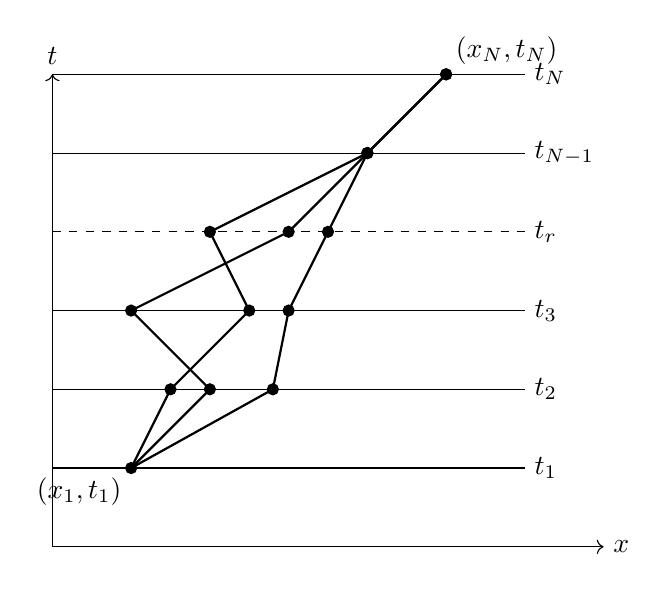
\begin{tikzpicture}
			
			% Draw axes
			\draw[->] (0,0) -- (7,0) node[right] {$x$};
			\draw[->] (0,0) -- (0,6) node[above] {$t$};
			
			% Time lines
			\draw (0,1) -- (6,1) node[right] {$t_1$};
			\draw (0,2) -- (6,2) node[right] {$t_2$};
			\draw (0,3) -- (6,3) node[right] {$t_3$};
			\draw[dashed] (0,4) -- (6,4) node[right] {$t_r$};
			\draw (0,5) -- (6,5) node[right] {$t_{N-1}$};
			\draw (0,6) -- (6,6) node[right] {$t_N$};
			
			% Different Paths
			\filldraw (1,1) circle (2pt) node[below left] {$(x_1, t_1)$};
			\filldraw (2,2) circle (2pt);
			\filldraw (1,3) circle (2pt);
			\filldraw (3,4) circle (2pt);
			\filldraw (4,5) circle (2pt);
			\filldraw (5,6) circle (2pt) node[above right] {$(x_N, t_N)$};
			
			\filldraw (1.5,2) circle (2pt);
			\filldraw (2.5,3) circle (2pt);
			\filldraw (2,4) circle (2pt);
			\filldraw (4,5) circle (2pt);
			
			\filldraw (2.8,2) circle (2pt);
			\filldraw (3,3) circle (2pt);
			\filldraw (3.5,4) circle (2pt);
			\filldraw (4,5) circle (2pt);
			\filldraw (5,6) circle (2pt);
			
			\draw[thick] (1,1) -- (2,2) -- (1,3) -- (3,4) -- (4,5) -- (5,6);
			\draw[thick] (1,1) -- (1.5,2) -- (2.5,3) -- (2,4) -- (4,5);
			\draw[thick] (1,1) -- (2.8,2) -- (3,3) -- (3.5,4) -- (4,5) -- (5,6);
		\end{tikzpicture}
	\end{center}
\end{figure}

在进一步进行之前, 在这里评述一下在经典力学中这些路径怎么出现是很有用的. 假定有一个受到可由位势 $V\left( x\right)$ 导出的力场作用的粒子. 经典的拉格朗日量记为
\begin{equation}
	{L}_{\text{经典 }}\left( {x,\dot{x}}\right) = \frac{m{\dot{x}}^{2}}{2} - V\left( x\right)
\end{equation}
给定了端点 $\left( {{x}_{1},{t}_{1}}\right)$ 和 $\left( {{x}_{N},{t}_{N}}\right)$ 的拉格朗日量,在经典力学中并不去考虑任何连接 $\left( {{x}_{1},{t}_{1}}\right)$ 和 $\left( {{x}_{N},{t}_{N}}\right)$ 的路径. 相反,存在一条唯一的路径对应于经典粒子的实际运动. 例如, 给定
\begin{equation}
	V\left( x\right) = {mgx},\;\left( {{x}_{1},{t}_{1}}\right) = \left( {h,0}\right) ,\;\left( {{x}_{N},{t}_{N}}\right) = ( {0,\sqrt{\frac{2h}{g}}})
\end{equation}
其中 $h$ 可以代表 Pisa 斜塔的高度,在 ${xt}$ 平面上的经典路径只能是
\begin{equation}
	x = h - \frac{g{t}^{2}}{2}
\end{equation}
更为普遍的是, 按照哈密顿原理, 这条唯一的路径是使经典拉格朗日量的时间积分定义的作用量取最小值的路径
\begin{equation}
	\delta \int_{{t}_{1}}^{{t}_{2}}{\d t}{L}_{\text{经典 }}\left( {x,\dot{x}}\right) = 0
\end{equation}
由它可以求得拉格朗日运动方程.
\subsection*{费曼的公式化表述}
经典力学与量子力学之间的基本差别现在应当清晰了. 在经典力学中,在 ${xt}$ 平面上有一条确定的路径与粒子的运动联系在一起, 而相比之下, 在量子力学中所有可能的路径都不可避免地起作用,包括那些与经典路径没有任何共同之处的路径. 然而,在 $\hbar \rightarrow$ 0 的极限下, 我们必须设法能够以光滑的方式重新产生经典力学. 我们如何实现这一点呢?

作为普林斯顿大学的一名年轻的研究生, 费曼试图攻克这一难题. 在寻找可能的线索时, 据说他被 Dirac 书中一段不可思议的评注迷住了, 用我们的记号, 它相当于下列说法
\begin{equation}
	\exp \left\lbrack {i\int_{{t}_{1}}^{{t}_{2}}\frac{{\d t}{L}_{\text{经典 }}\left( {x,\dot{x}}\right) }{\hbar }}\right\rbrack \text{ 对应于 }\left\langle {{x}_{2},{t}_{2} | {x}_{1},{t}_{1}}\right\rangle
\end{equation}
费曼试图理解这个评注. “对应于” 与 “等于” 或者 “正比于” 是一回事吗? 这种做法导致他构想出了一种基于路径积分的量子力学时空方法.

在费曼的公式化表述中, 经典作用量起着非常重要的作用. 为了简洁起见, 我们引进一种新的记号:
\begin{equation}
	S\left( {n, n - 1}\right) \equiv \int_{{t}_{n - 1}}^{{t}_{n}}{\d t}{L}_{\text{经典 }}\left( {x,\dot{x}}\right)
\end{equation}
由于 ${L}_{\text{经典 }}$ 是 $x$ 和 $x$ 的函数,只有在规定了一条沿着它做积分的确定的路径之后,才能把 $S\left( {n, n - 1}\right)$ 确定下来. 因此,尽管在这个记号中路径相关性并不明显,人们相信在计算这个积分时, 我们正在考虑一条特殊的路径. 现在想象我们正沿着某条指定的路径. 我们把注意力集中在沿着这条路径的一小分段上,比如在 $\left( {{x}_{n - 1},{t}_{n - 1}}\right)$ 和 $\left( {{x}_{n},{t}_{n}}\right)$ 之间的一段. 按照狄拉克的做法,要求我们把 $\exp \left\lbrack {{iS}\left( {n, n - 1}\right) /\hbar }\right\rbrack$ 与这一小段联系起来. 沿着这条准备跟踪的确定路径, 我们把这类表示式依次相乘得到
\begin{equation}
	\mathop{\prod }\limits_{{n = 2}}^{N}\exp \left\lbrack \frac{{iS}\left( {n, n - 1}\right) }{\hbar }\right\rbrack = \exp \left\lbrack {\left( \frac{i}{\hbar }\right) \mathop{\sum }\limits_{{n = 2}}^{N}S\left( {n, n - 1}\right) }\right\rbrack = \exp \left\lbrack \frac{{iS}\left( {N,1}\right) }{\hbar }\right\rbrack
\end{equation}
该式还没有给出 $\left\langle {{x}_{\mathrm{N}},{t}_{\mathrm{N}} | {x}_{1},{t}_{1}}\right\rangle$ ; 更确切地讲,这个方程是我们已考虑的特殊路径对 $\left\langle {{x}_{\mathrm{N}},{t}_{\mathrm{N}} | {x}_{1},{t}_{1}}\right\rangle$ 的贡献. 我们还必须对 ${x}_{2},{x}_{3},\cdots ,{x}_{\mathrm{N} - 1}$ 求积分. 与此同时,利用结合性, 我们让 ${t}_{n - 1}$ 和 ${t}_{n}$ 之间的时间间隔为无穷小. 于是在某种意义上, $\left\langle {{x}_{N},{t}_{N} | {x}_{1},{t}_{1}}\right\rangle$ 的候选表示式可以写成
\begin{equation}
	\left\langle {{x}_{N},{t}_{N} | {x}_{1},{t}_{1}}\right\rangle \sim \mathop{\sum }\limits_{\text{所有路径 }}\exp \left\lbrack \frac{{iS}\left( {N,1}\right) }{\hbar }\right\rbrack
\end{equation}
其中求和跑遍一个不可数的无穷大的路径集合\footnote{当然,这在数学上不太好说的通,至于如何合理化,那就变成了数学家的问题了.}!

在给出更精确的公式表示之前, 让我们看一下顺着这条思路的考虑在经典极限下是否有意义. 当 $\hbar \rightarrow 0$ 时,上式中的指数项振荡得非常剧烈,因此来自相邻路径的各种贡献间有着相消的倾向. 这是因为,作为 $\hbar$ 很小的结果,某个确定路径的 $\exp \left\lbrack {{iS}/\hbar }\right\rbrack$ 与稍微不同路径的 $\exp \left\lbrack {{iS}/\hbar }\right\rbrack$ 有着非常不同的相位. 因此,当 $\hbar$ 可以看作一个小量时,绝大多数路径没有贡献. 但是, 有一个\textbf{重要的例外}.

假定我们考虑一条路径, 它满足
\begin{equation}
	{\delta S}\left( {N,1}\right) = 0
\end{equation}
其中 $S$ 的变化是由于在保持端点固定情况下路径的略微形变. 这正是由哈密顿原理所决定的经典路径. 我们把满足上式的 $S$ 表示为 ${S}_{\text{最小}}$. 现在试着把经典路径做一点小的形变. 得到的 $S$ 在形变的第一级仍然等于 ${S}_{\text{最小}}$ . 这意味着即使$\hbar$很小,当我们稍微偏离经典路径时,$\exp\left\lbrack{{iS}/\hbar}\right\rbrack$ 的相位也不会变得太大.作为一个结果,只要我们停留在经典路径附近,则相邻路径之间的相干相加就有可能.在 $\hbar \rightarrow 0$的极限下,主要的贡献一定来自包含经典路径的一条非常狭窄的带子 (或者在更高维时的一根管子). 基于狄拉克不可思议的评注,我们 (或费曼) 的猜测很有道理,因为在 $\hbar \rightarrow 0$ 的极限下,经典路径被挑选了出来.为了更精确地阐述费曼的猜测,让我们回到 $\left\langle {{x}_{n},{t}_{n} | {x}_{n - 1},{t}_{n - 1}}\right\rangle$ , 其中的时间差 ${t}_{n} - {t}_{n - 1}$ 被假定为无穷小. 我们写出
\begin{equation}
	\left\langle {{x}_{n},{t}_{n} | {x}_{n - 1},{t}_{n - 1}}\right\rangle = \left\lbrack \frac{1}{w\left( {\Delta t}\right) }\right\rbrack \exp \left\lbrack \frac{{iS}\left( {n, n - 1}\right) }{\hbar }\right\rbrack
\end{equation}
其中的 $S\left( {n, n - 1}\right)$ 马上就在 ${\Delta t} \rightarrow 0$ 的极限下计算. 注意,我们插入了一个权重因子 $1/w\left( {\Delta t}\right)$ , 并假定它只依赖于时间间隔 ${t}_{n} - {t}_{n - 1}$ ,而不依赖于 $V\left( x\right)$ . 由量纲分析可清楚地看到需要这样一个因子,按照我们把位置本征右矢归一化的方法, $\left\langle {{x}_{n},{t}_{n} | {x}_{n - 1},{t}_{n - 1}}\right\rangle$ 必须具有 $1/($ 长度)的量纲.

现在我们看一下式中的指数. 我们的任务是计算 $S\left( {n, n - 1}\right)$ 在 ${\Delta t} \rightarrow 0$ 时的极限. 因为时间间隔如此之小,可以合理地对连接 $\left( {{x}_{n - 1},{t}_{n - 1}}\right)$ 和 $\left( {{x}_{n},{t}_{n}}\right)$ 的路径做直线近似:
\begin{equation}
	\begin{aligned}
		S\left( {n, n - 1}\right) &= \int_{{t}_{n - 1}}^{{t}_{n}}{\d t}\left\lbrack {\frac{m{\dot{x}}^{2}}{2} - V\left( x\right) }\right\rbrack\\
		&= {\Delta t}\left\{ {\left( \frac{m}{2}\right) {\left\lbrack \frac{\left( {x}_{n} - {x}_{n - 1}\right) }{\Delta t}\right\rbrack }^{2} - V\left( \frac{\left( {x}_{n} + {x}_{n - 1}\right) }{2}\right) }\right\}
	\end{aligned}
\end{equation}
作为一个例子,我们具体考虑自由粒子的情况,此时 $V = 0$ . 现在方程式变成
\begin{equation}
	\left\langle {{x}_{n},{t}_{n} | {x}_{n - 1},{t}_{n - 1}}\right\rangle = \left\lbrack \frac{1}{w\left( {\Delta t}\right) }\right\rbrack \exp \left\lbrack \frac{{im}{\left( {x}_{n} - {x}_{n - 1}\right) }^{2}}{2\hbar {\Delta t}}\right\rbrack
\end{equation}
我们看到, 这里出现的指数与自由粒子传播子表示式中的指数完全一样. 对于简谐振子, 读者可做出类似的比较.
早些时候我们曾指出过,在式中出现的权重因子 $1/w\left( {\Delta t}\right)$ 被假定不依赖于 $V\left( x\right)$ ,因此我们也可以用自由粒子求出它. 注意到,在 $\delta$ 函数的意义上,海森堡绘景中等时位置本征右矢的正交归一性
\begin{equation}
	\left\langle {{x}_{n},{t}_{n} | {x}_{n - 1},{t}_{n - 1}}\right\rangle {\left. \right| }_{{t}_{n} = {t}_{n - 1}} = \delta \left( {{x}_{n} - {x}_{n - 1}}\right)
\end{equation}
我们得到
\begin{equation}
	\frac{1}{w\left( {\Delta t}\right) } = \sqrt{\frac{m}{{2\pi i}\hbar {\Delta t}}}
\end{equation}
其中我们用到了
\begin{equation}
	\int_{-\infty }^{\infty }{\d \xi }\exp \left( \frac{{im}{\xi }^{2}}{2\hbar {\Delta t}}\right) = \sqrt{\frac{{2\pi i}\hbar {\Delta t}}{m}}
\end{equation}
和
\begin{equation}
	\mathop{\lim }\limits_{{{\Delta t} \rightarrow 0}}\sqrt{\frac{m}{{2\pi i}\hbar {\Delta t}}}\exp \left( \frac{{im}{\xi }^{2}}{2\hbar {\Delta t}}\right) = \delta \left( \xi \right)
\end{equation}
当然, 这个权重因子可以从自由粒子传播子表示式预料得到.

概括起来,当 ${\Delta t} \rightarrow 0$ 时,我们得到
\begin{equation}
	\left\langle {{x}_{n},{t}_{n} | {x}_{n - 1},{t}_{n - 1}}\right\rangle = \sqrt{\frac{m}{{2\pi i}\hbar {\Delta t}}}\exp \left\lbrack \frac{{iS}\left( {n, n - 1}\right) }{\hbar }\right\rbrack
\end{equation}
在 ${t}_{\mathrm{N}} - {t}_{1}$ 有限的情况下,跃迁振幅的最后表示式为
\begin{equation}
	\begin{aligned}
		\left\langle {{x}_{N},{t}_{N} | {x}_{1},{t}_{1}}\right\rangle &= \mathop{\lim }\limits_{{N \rightarrow \infty }}{\left( \frac{m}{{2\pi i}\hbar {\Delta t}}\right) }^{\left( {N - 1}\right) /2} \\
		&\times \int \d{x}_{N - 1}\int \d{x}_{N - 2}\cdots \int \d{x}_{2}\mathop{\prod }\limits_{{n = 2}}^{N}\exp \left\lbrack \frac{{iS}\left( {n, n - 1}\right) }{\hbar }\right\rbrack
	\end{aligned}
\end{equation}
其中, ${x}_{N}$ 和 ${t}_{N}$ 是固定的并取了 $N \rightarrow \infty$ 的极限. 通常定义一类新的多维(事实上,无穷维) 积分算符
\begin{equation}
	\int_{{x}_{1}}^{{x}_{N}}\mathcal{d}\left\lbrack {x\left( t\right) }\right\rbrack \equiv \mathop{\lim }\limits_{{N \rightarrow \infty }}{\left( \frac{m}{{2\pi i}\hbar {\Delta t}}\right) }^{\left( {N - 1}\right) /2}\int \d{x}_{N - 1}\int \d{x}_{N - 2}\cdots \int \d{x}_{2}
\end{equation}
并把其写成
\begin{equation}
	\left\langle {{x}_{N},{t}_{N} | {x}_{1},{t}_{1}}\right\rangle = \int_{{x}_{1}}^{{x}_{N}}\mathcal{d}\left\lbrack {x\left( t\right) }\right\rbrack \exp \left\lbrack {i\int_{{t}_{1}}^{{t}_{N}}{\d t}\frac{{L}_{\text{经典 }}\left( {x,\dot{x}}\right) }{\hbar }}\right\rbrack
\end{equation}
这个表达式称为\textbf{费曼路径积分}. 它作为对所有可能的路径求和的意义应当从式中清晰地看到.

我们求得上式的步骤并不意味着是一种推导. 相反, 我们 (遵循费曼) 尝试了一种基于路径概念的量子力学新形式, 它是以狄拉克不可思议的评注为动机的. 我们从常规量子力学形式那里借用的仅有的一些思想是: (1) 叠加原理 (用在各种可选路径贡献的求和); (2) 跃迁振幅结合性; (3) 在 $\hbar \rightarrow 0$ 极限时的经典对应.

尽管我们对于自由粒子情况求得的结果与常规理论的结果相同, 但从迄今为止我们已经做的一切明显可见: 费曼形式完全等价于薛定谔波动方程. 我们通过证明费曼的 $\left\langle {x}_{\mathrm{N}}\right.$ , ${t}_{\mathrm{N}}\left| {{x}_{1},{t}_{1}}\right\rangle$ 表达式确实满足以 ${x}_{\mathrm{N}},{t}_{\mathrm{N}}$ 为变量的薛定谔时间相关波动方程,就如同之前所定义的传播子所做的那样, 来结束这一节.

我们由
\begin{equation}
	\begin{aligned}
		\left\langle {{x}_{N},{t}_{N} | {x}_{1},{t}_{1}}\right\rangle &= \int \d{x}_{N - 1}\left\langle {{x}_{N},{t}_{N} | {x}_{N - 1},{t}_{N - 1}}\right\rangle \left\langle {{x}_{N - 1},{t}_{N - 1} | {x}_{1},{t}_{1}}\right\rangle\\
		&= \int_{-\infty }^{\infty }d{x}_{N - 1}\sqrt{\frac{m}{{2\pi i}\hbar {\Delta t}}}\exp \left\lbrack {\left( \frac{im}{2\hbar }\right) \frac{{\left( {x}_{N} - {x}_{N - 1}\right) }^{2}}{\Delta t} - \frac{iV\Delta t}{\hbar }}\right\rbrack\\
		&\times \left\langle {{x}_{N - 1},{t}_{N - 1} | {x}_{1},{t}_{1}}\right\rangle
	\end{aligned}
\end{equation}
开始,其中我们假定了 ${t}_{N} - {t}_{N - 1}$ 是无穷小. 引入
\begin{equation}
	\xi = {x}_{N} - {x}_{N - 1}
\end{equation}
且设 ${x}_{N} \rightarrow x$ 和 ${t}_{N} \rightarrow t + {\Delta t}$ ,我们得到
\begin{equation}
	\left\langle {x, t + {\Delta t} | {x}_{1},{t}_{1}}\right\rangle = \sqrt{\frac{m}{{2\pi i}\hbar {\Delta t}}}\int_{-\infty }^{\infty }{\d \xi }\exp \left( {\frac{{im}{\xi }^{2}}{2\hbar {\Delta t}} - \frac{iV\Delta t}{\hbar }}\right) \left\langle {x - \xi, t | {x}_{1},{t}_{1}}\right\rangle
\end{equation}
正如显而易见的,在 ${\Delta t} \rightarrow 0$ 的极限下,对该积分的主要贡献来自 $\xi \simeq 0$ 的区域. 因此可以合理地使用 $\xi$ 的幂来展开 $\left\langle {x - \xi, t | {x}_{1},{t}_{1}}\right\rangle$ . 我们还用 ${\Delta t}$ 的幂来展开 $\langle x, t$ $+ {\Delta t}\left| {{x}_{1},{t}_{1}}\right\rangle$ 和 $\exp \left( {-{iV\Delta t}/\hbar }\right)$ ,于是
\begin{equation}
	\begin{aligned}
		\left\langle {x, t | {x}_{1},{t}_{1}}\right\rangle + {\Delta t}\frac{\partial }{\partial t}\left\langle {x, t | {x}_{1},{t}_{1}}\right\rangle &= \sqrt{\frac{m}{{2\pi i}\hbar {\Delta t}}}\int_{-\infty }^{\infty }{\d \xi }\exp \left( \frac{{im}{\xi }^{2}}{2\hbar {\Delta t}}\right) \left( {1 - \frac{iV\Delta t}{\hbar } + \cdots }\right)\\
		&\times \left\lbrack {\left\langle {x, t | {x}_{1},{t}_{1}}\right\rangle + \left( \frac{{\xi }^{2}}{2}\right) \frac{{\partial }^{2}}{\partial {x}^{2}}\left\langle {x, t | {x}_{1},{t}_{1}}\right\rangle + \cdots }\right\rbrack
	\end{aligned}
\end{equation}
其中我们丢掉了 $\xi$ 的线性项,因为当对 $\xi$ 求积分时它为零. 由于 (2.6.45a) 式,上式左边的 $\left\langle {x, t | {x}_{1},{t}_{1}}\right\rangle$ 项正好与右边的领头项相对应. 把 ${\Delta t}$ 的一级项收集在一起,我们得到
\begin{equation}
	{\Delta t}\frac{\partial }{\partial t}\left\langle {x, t | {x}_{1},{t}_{1}}\right\rangle = \left( \sqrt{\frac{m}{{2\pi i}\hbar {\Delta t}}}\right) \left( \sqrt{2\pi }\right) {\left( \frac{i\hbar {\Delta t}}{m}\right) }^{3/2}\frac{1}{2}\frac{{\partial }^{2}}{\partial {x}^{2}}\left\langle {x, t | {x}_{1},{t}_{1}}\right\rangle- \left( \frac{i}{\hbar }\right) {\Delta tV}\left\langle {x, t | {x}_{1},{t}_{1}}\right\rangle
\end{equation}
其中我们用到了
\begin{equation}
	\int_{-\infty }^{\infty }{\d \xi }{\xi }^{2}\exp \left( \frac{{im}{\xi }^{2}}{2\hbar {\Delta t}}\right) = \sqrt{2\pi }{\left( \frac{i\hbar {\Delta t}}{m}\right) }^{3/2}
\end{equation}
就这样,我们看到 $\left\langle {x, t | {x}_{1},{t}_{1}}\right\rangle$ 满足薛定谔时间相关波动方程
\begin{equation}
	i\hbar \frac{\partial }{\partial t}\left\langle {x, t | {x}_{1},{t}_{1}}\right\rangle = - \left( \frac{{\hbar }^{2}}{2m}\right) \frac{{\partial }^{2}}{\partial {x}^{2}}\left\langle {x, t | {x}_{1},{t}_{1}}\right\rangle + V\left\langle {x, t | {x}_{1},{t}_{1}}\right\rangle
\end{equation}
由此我们可以得到结论: 按照费曼的规定构建的 $\left\langle {x, t | {x}_{1},{t}_{1}}\right\rangle$ 和薛定谔波动力学中的传播子是相同的.

费曼基于路径积分的时空方法对于处理非相对论量子力学的实际问题并不太方便. 甚至对于简谐振子, 要明显地求出有关的路径积分也是相当麻烦的. 然而, 他的做法从概念观点上看是十分令人满意的. 通过把一组必然的合乎情理的要求强加到一个物理理论中, 我们必然被引导到一种等价于通常量子力学公式表示的形式. 
\section{位势和规范变换}
\subsection*{恒定位势}
在经典力学中众所周知位势的零点是没有任何物理意义的. 动力学变量随时间的变化,诸如 $\mathbf{x}\left( t\right)$ 和 $\mathbf{L}\left( t\right)$ ,不依赖于我们使用的是 $V\left( \mathbf{x}\right)$ 还是 $V\left( \mathbf{x}\right) + {V}_{0}$ ,其中的 ${V}_{0}$ 对空间和时间都是常数. 在牛顿第二定律中出现的力只依赖于位势的梯度, 一个可加的常数显然是没有关系的. 在量子力学中, 类似的情况是什么呢?

我们来看一下受位势约束的薛定谔绘景态右矢的时间演化. 令 $\left| {\alpha ,{t}_{0};t}\right\rangle$ 是 $V\left( \mathbf{x}\right)$ 存在时的一个态右矢,并且令 $\left| {\alpha ,{t}_{0};t}\right\rangle$ 是适合于
\begin{equation}
	\widetilde{V}\left( \mathbf{x}\right) = V\left( \mathbf{x}\right) + {V}_{0}
\end{equation}
的相应的态右矢. 确切地说,让我们约定,初始条件是在 $t = {t}_{0}$ 时,这两个右矢都与 $|\alpha \rangle$ 一致. 如果它们代表着同样的物理情况, 这总可以通过适当地选择相位实现. 回忆一下, $t$ 时刻的态右矢可以通过把时间演化算符 $\mathcal{U}\left( {t,{t}_{0}}\right)$ 作用在 ${t}_{0}$ 时刻的态右矢上求得,于是我们得到
\begin{equation}
	\begin{aligned}
		\left| {\alpha ,{t}_{0};t}\right\rangle &= \exp \left\lbrack {-i\left( {\frac{{\mathbf{p}}^{2}}{2m} + V\left( x\right) + {V}_{0}}\right) \frac{\left( t - {t}_{0}\right) }{\hbar }}\right\rbrack |\alpha \rangle\\
		&= \exp \left\lbrack \frac{-i{V}_{0}\left( {t - {t}_{0}}\right) }{\hbar }\right\rbrack \left| {\alpha ,{t}_{0};t}\right\rangle
	\end{aligned}
\end{equation}
换句话说,在 $\widetilde{V}$ 的影响下计算的右矢,其时间依赖关系仅差一个相因子 $\exp \left\lbrack {-i{V}_{0}\left( {t - {t}_{0}}\right) /\hbar }\right\rbrack$ . 对于定态,这意味着,如果用 $V\left( \mathbf{x}\right)$ 算得的时间依赖关系为 $\exp \left\lbrack {-{iE}\left( {t - {t}_{0}}\right) /\hbar }\right\rbrack$ ,则用 $V\left( \mathbf{x}\right) + {V}_{0}$ 算得的相应的时间依赖关系为 $\exp \left\lbrack {-i\left( {E + {V}_{0}}\right) \left( {t - {t}_{0}}\right) /\hbar }\right\rbrack$ . 换句话说,用 $\widetilde{V}$ 代替 $V$ 只意味着下列改变:
\begin{equation}
	E \rightarrow E + {V}_{0}
\end{equation}
这一点,或许读者马上就能猜到. 可观测量受到的影响,比如期望 $\langle \mathbf{x}\rangle$ 和 $\langle \mathbf{S}\rangle$ 的时间演化,总是依赖于能量差; 不管我们是用 $V\left( \mathbf{x}\right)$ 还是用 $V\left( \mathbf{x}\right) + {V}_{0}$ ,表征着期望的正弦时间依赖关系的波尔频率都是一样的. 一般来说, 倘若世界上每一个态右矢都乘上一个共同的因子 $\exp \left\lbrack {-i{V}_{0}\left( {t - {t}_{0}}\right) /\hbar }\right\rbrack$ ,则可观测量的期望可能没有任何差别.

虽然看上去这可能是很平庸的, 但这里我们看到了称之为规范变换的一类变换的第一个例子. 在我们约定中势能零点能的变化
\begin{equation}
	V\left( \mathbf{x}\right) \rightarrow V\left( \mathbf{x}\right) + {V}_{0}
\end{equation}
一定伴随着态右矢的一个变化
\begin{equation}
	\left| {\alpha ,{t}_{0};t}\right\rangle \rightarrow \exp \left\lbrack \frac{-i{V}_{0}\left( {t - {t}_{0}}\right) }{\hbar }\right\rbrack \left| {\alpha ,{t}_{0};t}\right\rangle
\end{equation}
当然, 这个变化意味着波函数有下列改变:
\begin{equation}
	\psi \left( {{\mathbf{x}}^{\prime }, t}\right) \rightarrow \exp \left\lbrack \frac{-i{V}_{0}\left( {t - {t}_{0}}\right) }{\hbar }\right\rbrack \psi \left( {{\mathbf{x}}^{\prime }, t}\right)
\end{equation}
接下来,我们考虑, ${V}_{0}$ 是空间均匀但随时间变化的. 我们很容易看到与其类似的表达式
\begin{equation}
	\left| {\alpha ,{t}_{0};t}\right\rangle \rightarrow \exp \left\lbrack {-i\int_{{t}_{0}}^{t}\d{t}^{\prime }\frac{{V}_{0}\left( {t}^{\prime }\right) }{\hbar }}\right\rbrack \left| {\alpha ,{t}_{0};t}\right\rangle
\end{equation}
物理上,用 $V\left( \mathbf{x}\right) + {V}_{0}$ 代替 $V\left( \mathbf{x}\right)$ 只不过意味着,在每个瞬间我们都选择了一个新的能量标度零点\footnote{尽管势能绝对标度的选取是任意的, 但势能差具有非平庸的物理意义.}.
\subsection*{电磁学中的规范变换}
现在让我们回到电磁学中出现的势. 我们考虑从时间无关的标量势和矢量势, $\phi \left( \mathbf{x}\right)$ 和 $\mathbf{A}\left( \mathbf{x}\right)$ ,导出的电场与磁场:
\begin{equation}
	\mathbf{E} = - \nabla \phi ,\;\mathbf{B} = \nabla \times \mathbf{A}
\end{equation}
一个电荷为 $e$ (对于电子 $e < 0$ ) 受到电磁场作用的粒子,由经典物理给出的哈密顿量为
\begin{equation}
	H = \frac{1}{2m}{\left( \mathbf{p} - \frac{e\mathbf{A}}{c}\right) }^{2} + {e\phi }
\end{equation}
在量子力学中 $\phi$ 和 $\mathbf{A}$ 被认为是带电粒子的位置算符 $\mathbf{x}$ 的函数. 因为 $\mathbf{p}$ 和 $\mathbf{A}$ 不对易,在解释时需要小心点. 最安全的做法是写成
\begin{equation}
	{\left( \mathbf{p} - \frac{e\mathbf{A}}{c}\right) }^{2} \rightarrow {p}^{2} - \left( \frac{e}{c}\right) \left( {\mathbf{p} \cdot \mathbf{A} + \mathbf{A} \cdot \mathbf{p}}\right) + {\left( \frac{e}{c}\right) }^{2}{\mathbf{A}}^{2}
\end{equation}
在这种形式下, 哈密顿量显然是厄米的.

为了研究一个受到 $\phi$ 和 $\mathbf{A}$ 作用的带电粒子的动力学,让我们首先在海森堡绘景中操作. 我们可以直接计算 $\mathbf{x}$ 的时间微商
\begin{equation}
	\frac{\d {x}_{i}}{\d t} = \frac{\left\lbrack {x}_{i}, H\right\rbrack }{i\hbar } = \frac{\left( {p}_{i} - e{A}_{i}/c\right) }{m}
\end{equation}
它显示本书中定义为平移生成元的算符 $\mathbf{p}$ 与 ${md}\mathbf{x}/{\d t}$ 不同. $\mathbf{p}$ 经常称为\textbf{正则动量},以示与运动学 (或力学) 动量的区别,后者用 $\Pi$ 标记:
\begin{equation}
	\Pi \equiv m\frac{\d \mathbf{x}}{\d t} = \mathbf{p} - \frac{e\mathbf{A}}{c}
\end{equation}
尽管对于正则动量我们有
\begin{equation}
	\left\lbrack {{p}_{i},{p}_{j}}\right\rbrack = 0
\end{equation}
力学动量的类似对易关系不为零. 相反, 我们有
\begin{equation}
	\left\lbrack {{\Pi }_{i},{\Pi }_{j}}\right\rbrack = \left( \frac{ihe}{c}\right) {\varepsilon }_{ijk}{B}_{k}
\end{equation}
这一点, 读者可以很容易证明. 把哈密顿量改写为
\begin{equation}
	H = \frac{{\Pi }^{2}}{2m} + {e\phi }
\end{equation}
并利用基本对易关系, 我们可以导出量子力学版本的洛伦兹 (Lorentz) 力, 即
\begin{equation}
	m\frac{{\d}^{2}\mathbf{x}}{\d{t}^{2}} = \frac{\d \Pi }{\d t} = e\left\lbrack {\mathbf{E} + \frac{1}{2c}\left( {\frac{\d \mathbf{x}}{\d t} \times \mathbf{B} - \mathbf{B} \times \frac{\d \mathbf{x}}{\d t}}\right) }\right\rbrack
\end{equation}
这就是海森堡绘景中,当 $\mathbf{E}$ 和 $\mathbf{B}$ 存在时,带电粒子的\textbf{埃伦费斯特定理}.

现在,我们研究具有 $\phi$ 和 $\mathbf{A}$ 的薛定谔波动方程. 我们的第一个任务是在 $\left\langle {\mathbf{x}}^{\prime }\right|$ 和 $\alpha ,{t}_{0}$ ; $t\rangle$ 之间夹入 $H$ . 唯一需要加以小心的项是
\begin{equation}
	\begin{aligned}
		\left\langle {{\mathbf{x}}^{\prime }\left| {\left\lbrack \mathbf{p} - \frac{e\mathbf{A}\left( \mathbf{x}\right) }{c}\right\rbrack }^{2}\right| \alpha ,{t}_{0};t}\right\rangle &= \left\lbrack {-i\hbar {\nabla }^{\prime } - \frac{e\mathbf{A}\left( {\mathbf{x}}^{\prime }\right) }{c}}\right\rbrack \left\langle {{\mathbf{x}}^{\prime }\left| \left\lbrack {\mathbf{p} - \frac{e\mathbf{A}\left( \mathbf{x}\right) }{c}}\right\rbrack \right| \alpha ,{t}_{0};t}\right\rangle\\
		&= \left\lbrack {-i\hbar {\nabla }^{\prime } - \frac{e\mathbf{A}\left( {\mathbf{x}}^{\prime }\right) }{c}}\right\rbrack \cdot \left\lbrack {-{ih}{\nabla }^{\prime } - \frac{e\mathbf{A}\left( {\mathbf{x}}^{\prime }\right) }{c}}\right\rbrack \left\langle {{\mathbf{x}}^{\prime } | \alpha ,{t}_{0};t}\right\rangle
	\end{aligned}
\end{equation}
需要强调的是,在最后一行中的第一个 ${\nabla }^{\prime }$ 既要对 $\left\langle {{\mathbf{x}}^{\prime } | \alpha ,{t}_{0};t}\right\rangle$ 微商,也要对 $\mathbf{A}\left( {\mathbf{x}}^{\prime }\right)$ 微商. 把这一切组合起来, 我们有
\begin{equation}
	\frac{1}{2m}\left\lbrack {-i\hbar {\nabla }^{\prime } - \frac{e\mathbf{A}\left( {\mathbf{x}}^{\prime }\right) }{c}}\right\rbrack \cdot \left\lbrack {-i\hbar {\nabla }^{\prime } - \frac{e\mathbf{A}\left( {\mathbf{x}}^{\prime }\right) }{c}}\right\rbrack \left\langle {{\mathbf{x}}^{\prime } | \alpha ,{t}_{0};t}\right\rangle+ {e\phi }\left( {\mathbf{x}}^{\prime }\right) \left\langle {{\mathbf{x}}^{\prime } | \alpha ,{t}_{0};t}\right\rangle = i\hbar \frac{\partial }{\partial t}\left\langle {{\mathbf{x}}^{\prime } | \alpha ,{t}_{0};t}\right\rangle
\end{equation}
从这个表达式我们很容易得到连续性方程
\begin{equation}
	\frac{\partial \rho }{\partial t} + {\nabla }^{\prime } \cdot \mathbf{j} = 0
\end{equation}
在那里,像以前一样 $\rho$ 是 ${\left| \psi \right| }^{2},\left\langle {{\mathbf{x}}^{\prime } | \alpha ,{t}_{0};t}\right\rangle$ 是 $\psi$ ,而对概率流 $\mathbf{j}$ 我们有
\begin{equation}
	\mathbf{j} = \left( \frac{\hbar }{m}\right) \operatorname{Im}\left( {{\psi }^{ * }{\nabla }^{\prime }\psi }\right) - \left( \frac{e}{mc}\right) \mathbf{A}{\left| \psi \right| }^{2}
\end{equation}
它正是我们由代换
\begin{equation}
	{\nabla }^{\prime } \rightarrow {\nabla }^{\prime } - \left( \frac{ie}{\hbar c}\right) \mathbf{A}
\end{equation}
所预期的. 若把波函数写成 $\sqrt{\rho }\exp \left( {{iS}/\hbar }\right)$,我们得到 $\mathbf{j}$ 的一个替代形式, 即
\begin{equation}
	\mathbf{j} = \left( \frac{\rho }{m}\right) \left( {\nabla S - \frac{e\mathbf{A}}{c}}\right)
\end{equation}
相比较,我们将发现, 这种形式在讨论超导、通量量子化等问题时是方便的. 我们还注意到,除去 $1/m$ 外, $\mathbf{j}$ 的空间积分就是运动学动量 (而不是正则动量) 的期望
\begin{equation}
	\int {\d}^{3}{x}^{\prime }\mathbf{j} = \frac{\langle \mathbf{p} - e\mathbf{A}/c\rangle }{m} = \langle \Pi \rangle /m
\end{equation}
现在我们是讨论电磁学中规范变换问题的时候了. 首先, 考虑
\begin{equation}
	\phi \rightarrow \phi + \lambda ,\;\mathbf{A} \rightarrow \mathbf{A}
\end{equation}
其中的 $\lambda$ 是个常数,这就是说,不依赖于 $\mathbf{x}$ 和 $t$ . $\mathbf{E}$ 和 $\mathbf{B}$ 二者显然都保持不变. 这个变换只意味着能量标度零点的变化,它是在本节开始时用过的一种可能性; 我们只不过用 ${e\phi }$ 代替了 $V$ . 我们已经讨论过了态右矢所需要的伴随变化,因此,我们不再赘述这个变换.

更有趣的是变换
\begin{equation}
	\phi \rightarrow \phi ,\;\mathbf{A} \rightarrow \mathbf{A} + \nabla \Lambda
\end{equation}
其中 $\Lambda$ 是 $\mathbf{x}$ 的函数. 在上面的变换下,静电磁场 $\mathbf{E}$ 和 $\mathbf{B}$ 是不变的.都是
\begin{equation}
	\phi \rightarrow \phi - \frac{1}{c}\frac{\partial \Lambda }{\partial t},\;\mathbf{A} \rightarrow \mathbf{A} + \nabla \Lambda
\end{equation}
的特殊情况, 它们保持由
\begin{equation}
	\mathbf{E} = - \nabla \phi - \frac{1}{c}\frac{\partial \mathbf{A}}{\partial t},\;\mathbf{B} = \nabla \times \mathbf{A}
\end{equation}
给出的 $\mathbf{E}$ 和 $\mathbf{B}$ 不变,但下面我们不考虑时间相关的场和势. 在本节的余下部分,术语规范变换指的都是这类变换.

在经典物理中, 诸如带电粒子轨道这样的可观测量效应不依赖所使用的规范一一即我们碰巧采用的特别选择的 $\Lambda$ . 考虑一个带电粒子处于沿 $z$ 方向的均匀磁场中
\begin{equation}
	\mathbf{B} = B\widehat{\mathbf{z}}
\end{equation}
这个磁场可以从
\begin{equation}
	{A}_{x} = \frac{-{By}}{2},\;{A}_{y} = \frac{Bx}{2},\;{A}_{z} = 0
\end{equation}
推导出来. 或者也可以从
\begin{equation}
	{A}_{x} = - {By},\;{A}_{y} = 0,\;{A}_{z} = 0
\end{equation}
推导出来. 第二种形式是通过
\begin{equation}
	\mathbf{A} \rightarrow \mathbf{A} - \nabla \left( \frac{Bxy}{2}\right)
\end{equation}
从第一种形式中求得的,它的确是规范变换的形式. 不管我们可能会用哪个 $\mathbf{A}$ ,具有一组给定初始条件的带电粒子的轨道都是相同的,它就是一条螺旋线——投影到 ${xy}$ 平面时的一个匀速圆周运动,同时叠加上沿 $z$ 方向的一个匀速直线运动. 然而,如果我们看一下 ${p}_{x}$ 和 ${p}_{y}$ ,结果则是很不一样的. 首先,当使用第二种形式时, ${p}_{x}$ 是个运动常数,而当使用第一种形式时它就不再是运动常数.

回顾哈密顿运动方程:
\begin{equation}
	\frac{\d {p}_{x}}{\d t} = - \frac{\partial H}{\partial x},\;\frac{\d {p}_{y}}{\d t} = - \frac{\partial H}{\partial y},\cdots
\end{equation}
一般说来,正则动量 $\mathbf{p}$ 不是一个规范不变量,即使我们针对的是同一个物理情况,它的数值仍依赖于所采用的特殊规范. 相比之下,跟踪粒子轨迹的运动学动量 $\Pi$ ,或 ${m\d}\mathbf{x}/{\d t}$ ,是一个规范不变量,这一点可以明确证明. 因为 $\mathbf{p}$ 和 ${md}\mathbf{x}/{\d t}$ 相关联, $\mathbf{p}$ 必须改变以补偿$\mathbf{A}$ 的变化.

现在我们回到量子力学. 我们相信, 在规范变换下要求量子力学中的期望具有类似于相应的经典量的行为方式是合理的,所以在规范变换下,预期 $\langle \mathbf{x}\rangle$ 和 $\langle \Pi \rangle$ 不变,而 $\langle \mathbf{p}\rangle$ 会变化.

让我们用 $|\alpha \rangle$ 表示 $\mathbf{A}$ 存在时的态右矢; 当用
\begin{equation}
	\widetilde{\mathbf{A}} = \mathbf{A} + \nabla \Lambda
\end{equation}
代替 $\mathbf{A}$ 时,同样物理情况下的态右矢用 $|\widetilde{\alpha }\rangle$ 表示. 这里的 $\Lambda$ ,和 $\mathbf{A}$ 一样,是位置算符 $\mathbf{x}$ 的函数. 我们的基本要求是
\begin{equation}
	\langle \alpha \left| \mathbf{x}\right| \alpha \rangle = \langle \widetilde{\alpha }\left| \mathbf{x}\right| \widetilde{\alpha }\rangle
\end{equation}
和
\begin{equation}
	\langle \alpha | \left( {\mathbf{p} - \frac{e\mathbf{A}}{c}}\right) | \alpha \rangle = \langle \widetilde{\alpha }| \left( {\mathbf{p} - \frac{e\widetilde{\mathbf{A}}}{c}}\right) | \widetilde{\alpha }\rangle
\end{equation}
此外, 像往常一样, 我们要求态右矢的模保持不变:
\begin{equation}
	\langle \alpha | \alpha \rangle = \langle \widetilde{\alpha } | \widetilde{\alpha }\rangle
\end{equation}
我们必须构建一个把 $\left| {\bar{\alpha }\rangle \text{和}}\right| \alpha \rangle$ 如下联系起来的算符 $\mathscr{G}$
\begin{equation}
	\left| {\widetilde{\alpha }\rangle = \mathscr{G}}\right| \alpha \rangle
\end{equation}
倘若
\begin{equation}
	\mathscr{G}^\dagger x\mathscr{G}= x
\end{equation}
和
\begin{equation}
	\mathscr{G}^\dagger\left( {\mathbf{p} - \frac{e\mathbf{A}}{c} - \frac{e\nabla \Lambda }{c}}\right) \mathscr{G} = \mathbf{p} - \frac{e\mathbf{A}}{c}
\end{equation}
则不变性都能得到保障. 我们断言
\begin{equation}
	\mathscr{G} = \exp \left\lbrack \frac{{ie\Lambda }\left( \mathbf{x}\right) }{\hbar c}\right\rbrack
\end{equation}
能满足这个要求.$\mathscr{G}$ 是幺正的且 $\mathbf{x}$ 与 $\mathbf{x}$ 的任意函数对易,则前面的式子显然满足. 至于最后一个式子, 只需指出
\begin{equation}
	\begin{aligned}
		\exp \left( \frac{-{ie\Lambda }}{\hbar c}\right) \mathbf{p}\exp \left( \frac{ie\Lambda }{\hbar c}\right) &= \exp \left( \frac{-{ie\Lambda }}{\hbar c}\right) \left\lbrack {\mathbf{p},\exp \left( \frac{ie\Lambda }{\hbar c}\right) }\right\rbrack + \mathbf{p}\\
		&= - \exp \left( \frac{-{ie\Lambda }}{\hbar c}\right) i\hbar \nabla \left\lbrack {\exp \left( \frac{ie\Lambda }{\hbar c}\right) }\right\rbrack + \mathbf{p}\\
		&= \mathbf{p} + \frac{e\nabla \Lambda }{c}
	\end{aligned}
\end{equation}
规范变换下的量子力学不变性还可以通过直接观察薛定谔方程来展示. 设 $\left| {\alpha ,{t}_{0};t}\right\rangle$ 是 $\mathbf{A}$ 存在时薛定谔方程的一个解:
\begin{equation}
	\left\lbrack {\frac{{\left( \mathbf{p} - e\mathbf{A}/c\right) }^{2}}{2m} + {e\phi }}\right\rbrack \left| {\alpha ,{t}_{0};t}\right\rangle = i\hbar \frac{\partial }{\partial t}\left| {\alpha ,{t}_{0};t}\right\rangle
\end{equation}
在 $\widetilde{\mathbf{A}}$ 存在时,相应的解必须满足
\begin{equation}
	\left\lbrack {\frac{{\left( \mathbf{p} - e\mathbf{A}/c - e\nabla \Lambda /c\right) }^{2}}{2m} + {e\phi }}\right\rbrack \left| {\alpha ,\widetilde{{t}_{0}};t}\right\rangle = i\hbar \frac{\partial }{\partial t}\left| {\alpha ,\widetilde{{t}_{0}};t}\right\rangle
\end{equation}
我们看到, 如果=把新的右矢取为
\begin{equation}
	\left| {\alpha ,{\widetilde{t}}_{0};t}\right\rangle = \exp \left( \frac{ie\Lambda }{\hbar c}\right) \left| {\alpha ,{t}_{0};t}\right\rangle
\end{equation}
则上面新的薛定谔方程将得到满足; 我们必须注意的是
\begin{equation}
	\exp \left( \frac{-{ie\Lambda }}{\hbar c}\right) {\left( \mathbf{p} - \frac{e\mathbf{A}}{c} - \frac{e\nabla \Lambda }{c}\right) }^{2}\exp \left( \frac{ie\Lambda }{\hbar c}\right) = {\left( \mathbf{p} - \frac{e\mathbf{A}}{c}\right) }^{2}
\end{equation}
相应的波函数通过
\begin{equation}
	\psi \left( {{\mathbf{x}}^{\prime }, t}\right) = \exp \left\lbrack \frac{{ie\Lambda }\left( {\mathbf{x}}^{\prime }\right) }{\hbar c}\right\rbrack \psi \left( {{\mathbf{x}}^{\prime }, t}\right)
\end{equation}
关联起来,其中的 $\mathbf{\Lambda }\left( {\mathbf{x}}^{\prime }\right)$ 现在是位置矢量本征值 ${\mathbf{x}}^{\prime }$ 的一个实函数. 当然,通过直接代入以 $\mathbf{A} + \nabla \Lambda$ 代替 $\mathbf{A}$ 的薛定谔波动方程,也可以证明这一点. 从 $\rho$ 和 $S$ 的角度来讲,我们看到, $\rho$ 是不变的,而 $S$ 被修改为
\begin{equation}
	S \rightarrow S + \frac{e\Lambda }{c}
\end{equation}
这一点是非常合理的, 因为我们发现所给出的概率流是规范不变的.

总之, 当对同样的物理情况使用不同规范下的矢量势时, 相应的态右矢 (或波函数) 必定是不同的. 然而, 仅仅需要简单的改变; 只要把老的右矢 (或老的波函数) 乘以 $\exp \left\lbrack {{ie\Lambda }\left( \mathbf{x}\right) /\hbar c}\right\rbrack \left( {\exp \left\lbrack {{ie\Lambda }\left( {\mathbf{x}}^{\prime }\right) /\hbar c}\right\rbrack }\right)$ ,就可以从由 $\mathbf{A}$ 确定的规范变到另一个由 $\mathbf{A} + \nabla \Lambda$ 确定的规范. 在其期望依赖于特殊规范的这样一种意义上, 定义为平移生成元的\textbf{正则动量}显然是规范相关的, 而\textbf{运动学动量}和概率流都是规范不变的.

考虑在 $\mathbf{x}$ 处的某个位置的函数 $F\left( \mathbf{x}\right)$ . 在相邻的点我们显然有
\begin{equation}
	F\left( {\mathbf{x} + \d\mathbf{x}}\right) \simeq F\left( \mathbf{x}\right) + \left( {\nabla F}\right) \cdot\d\mathbf{x}
\end{equation}
但是假定当我们从 $\mathbf{x}$ 到 $\mathbf{x} + \d\mathbf{x}$ 时做了一个标度变化如下:
\begin{equation}
	{\left. 1\right| }_{\text{在x处 }} \rightarrow {\left. \left\lbrack 1 + \sum \left( \mathbf{x}\right) \cdot \d\mathbf{x}\right\rbrack \right| }_{\text{在x } + \d\mathbf{x}\text{ 处 }}
\end{equation}
那么,我们必须重新标度 $\mathrm{F}\left( \mathbf{x}\right)$
\begin{equation}
	{\left. F\left( \mathbf{x} + \d\mathbf{x}\right) \right| }_{\text{重新标度后 }} \simeq F\left( \mathbf{x}\right) + \left\lbrack {\left( {\nabla + \mathbf{\sum }}\right) F}\right\rbrack \cdot \d\mathbf{x}
\end{equation}
组合 $\nabla + \mathbf{\sum }$ 类似于在之前见到过的规范不变组合
\begin{equation}
	\nabla - \left( \frac{ie}{\hbar c}\right) \mathbf{A}
\end{equation}
除不存在 $i$ 之外.  我们坚持了术语规范不变性, 尽管其的量子力学类比
\begin{equation}
	{\left. 1\right| }_{\text{在x处 }} \rightarrow {\left. \left\lbrack 1 - \left( \frac{ie}{\hbar c}\right) \mathbf{A} \cdot \d\mathbf{x}\right\rbrack \right| }_{\text{在x+}\d x\text{处}}
\end{equation}
将实际对应于 “相位改变” 而不是 “标度改变”.
\subsection*{阿哈罗诺夫-玻姆效应}
在量子力学中矢量势的使用有很多深远影响, 我们现在准备讨论其中的一些. 我们从一个看似平淡无奇的问题开始.

考虑一个中空的圆柱形壳. 我们假定一个电荷为 $e$ 的粒子能够完全地被禁闭在这个刚性壁壳的内部. 要求波函数在内壁 $\left( {\rho = {\rho }_{a}}\right)$ 和外壁 $\left( {\rho = {\rho }_{b}}\right)$ 上为零, 在顶部和底部也为零. 这是一个数学物理中求解能量本征值的简单的边值问题.

让我们现在考虑一个修改过的装置, 在那里一个圆柱壳把一个均匀磁场包围了起来, 如图 2.11b 所示. 特别是,你可以想象一个非常长的螺线管插到中间的孔中,以致没有任何磁场泄漏到 $\rho \geq {\rho }_{a}$ 的区域. 波函数的边界条件取为与以前的一样; 并且假定壁是刚性的. 凭直觉,我们可以猜测到能谱不会改变,因为 $\mathbf{B} \neq 0$ 的区域完全不可能达到被禁闭在壳内的带电粒子. 然而, 量子力学告诉我们这个猜测不对.

尽管磁场在内部区域为零, 那里的矢量势不为零. 利用斯托克斯 (Stokes) 定理, 我们可以推知要产生磁场 $\mathbf{B}\left( { = B\widehat{\mathbf{z}}}\right)$ 所需的矢量势为
\begin{equation}
	\mathbf{A} = \left( \frac{B{\rho }_{u}^{2}}{2\rho }\right) \widehat{\phi }
\end{equation}
其中的 $\widetilde{\phi }$ 是沿方位角增加方向的单位矢量. 在试图求解薛定谔方程以找到这个新问题的能量本征值时,我们仅需要用 $\nabla - \left( {{ie}/\hbar c}\right) \mathbf{A}$ 代替梯度 $\nabla$ ; 我们可以在柱坐标系中把对 $\phi$ 的偏微商做如下代换来实现这一点:
\begin{equation}
	\frac{\partial }{\partial \phi } \rightarrow \frac{\partial }{\partial \phi } - \left( \frac{ie}{\hbar c}\right) \frac{B{\rho }_{a}^{2}}{2}
\end{equation}
这里要回顾柱坐标系中梯度的表示式:
\begin{equation}
	\nabla = \widehat{\mathbf{\rho }}\frac{\partial }{\partial \rho } + \widehat{\mathbf{z}}\frac{\partial }{\partial z} + \widehat{\mathbf{\phi }}\frac{1}{\rho }\frac{\partial }{\partial \phi }
\end{equation}

图 2.11 空心圆柱壳 (a) 没有磁场, (b) 有一个均匀磁场.

(2.7.63) 式的代换导致了能谱可观测的变化, 这一点读者可以明显地证明. 这是非常引人瞩目的, 因为粒子从来没有 “接触” 到磁场; 在这个问题中粒子受到的洛伦兹力恒为零, 然而能级却取决于粒子不可达到的孔区内的磁场是否有限.

我们刚刚处理的这个问题是通常被称作阿哈罗诺夫-玻姆效应 ${}^{ * }$ 的束缚态版本. 现在我们着手讨论阿哈罗诺夫-玻姆效应自身的原始形式. 考虑一个电荷为 $e$ 的粒子,经过一个非常长的不可穿透的圆柱体之上或之下, 如图 2.12 所示. 圆柱体内部是一个平行于圆柱体轴的磁场, 而该轴垂直于图 2.12 的平面. 所以粒子的上路径和下路径包围了磁通量. 我们的目标是研究在相互作用区 $\mathrm{B}$ 找到粒子的概率如何依赖于磁通量.

图 2.12 阿哈罗诺夫-玻姆效应

尽管可以通过比较 B 存在和不存在时薛定谔方程的解来处理这个问题, 为了便于教学,我们宁可采用费曼路径积分方法. 设 ${\mathbf{x}}_{1}$ 和 ${\mathbf{x}}_{N}$ 分别是源区 $\mathrm{A}$ 和干涉区 $\mathrm{B}$ 中的两个有代表性的点. 从经典力学得知, 存在磁场时的拉格朗日量可从不存在磁场时的拉格朗日量 (用 ${L}_{\text{经典 }}^{\left( 0\right) }$ 表示) 得到
\begin{equation}
	{L}_{\text{经典 }}^{\left( 0\right) } = \frac{m}{2}{\left( \frac{\d \mathbf{x}}{\d t}\right) }^{2} \rightarrow {L}_{\text{经典 }}^{\left( 0\right) } + \frac{e}{c}\frac{\d \mathbf{x}}{\d t} \cdot \mathbf{A}
\end{equation}
然后,对于从 $\left( {{\mathbf{x}}_{n - 1},{t}_{n - 1}}\right)$ 到 $\left( {{\mathbf{x}}_{n},{t}_{n}}\right)$ 的某段确定的路径单元,作用量相应的改变由下式给出
\begin{equation}
	{S}^{\left( 0\right) }\left( {n, n - 1}\right) \rightarrow {S}^{\left( 0\right) }\left( {n, n - 1}\right) + \frac{e}{c}\int_{{t}_{n - 1}}^{{t}_{n}}{\d t}\left( \frac{\d \mathbf{x}}{\d t}\right) \cdot \mathbf{A}
\end{equation}
而最后的这个积分可以写成
\begin{equation}
	\frac{e}{c}\int_{{t}_{n - 1}}^{{t}_{n}}{\d t}\left( \frac{\d \mathbf{x}}{\d t}\right) \cdot \mathbf{A} = \frac{e}{c}\int_{{x}_{n - 1}}^{{x}_{n}}\mathbf{A} \cdot \d\mathbf{s}
\end{equation}
其中的 $\d\mathbf{s}$ 是沿着这段路径单元的微分线元,因此当我们考虑从 ${\mathbf{x}}_{1}$ 到 ${\mathbf{x}}_{N}$ 的全部贡献时, 有下列的改变
\begin{equation}
	\prod \exp \left\lbrack \frac{i{S}^{\left( 0\right) }\left( {n, n - 1}\right) }{\hbar }\right\rbrack \rightarrow \left\{ {\prod \exp \left\lbrack \frac{i{S}^{\left( 0\right) }\left( {n, n - 1}\right) }{\hbar }\right\rbrack }\right\} \exp \left( {\frac{ie}{\hbar c}\int_{{\mathbf{x}}_{1}}^{{\mathbf{x}}_{N}}\mathbf{A} \cdot d\mathbf{s}}\right)
\end{equation}
所有这一切只是对于一条特殊的路径, 比如从圆柱体上部通过的路径. 我们还必须对所有的可能路径求和, 这似乎是一个令人生畏的任务. 幸运的是, 我们从电磁学理论知道, $\int \mathbf{A} \cdot d\mathbf{s}$ 的线积分与路径无关. 即,只要一对不同的路径形成的圈不包围磁通量,它就仅依赖于两个端点. 作为结果,由于 $\mathbf{A} \neq 0$ 所有从圆柱体上部通过的路径的贡献都由一个共同的相位因子给出; 类似地, 来自所有从圆柱体下部通过的路径的贡献都将乘以另一个共同的相位因子. 用路径积分符号, 对于整个跃迁振幅我们有
\begin{equation}
	\begin{aligned}
		&\int_{\mathrm{E}}\mathcal{d}\left\lbrack {\mathbf{x}\left( t\right) }\right\rbrack \exp \left\lbrack \frac{i{S}^{\left( 0\right) }\left( {N,1}\right) }{\hbar }\right\rbrack + \int_{\mathrm{F}}\mathcal{d}\left\lbrack {\mathbf{x}\left( t\right) }\right\rbrack \exp \left\lbrack \frac{i{S}^{\left( 0\right) }\left( {N,1}\right) }{\hbar }\right\rbrack\\
		&\rightarrow \int_{E}\mathcal{d}\left\lbrack {\mathbf{x}\left( t\right) }\right\rbrack \exp \left\lbrack \frac{i{S}^{\left( 0\right) }\left( {N,1}\right) }{\hbar }\right\rbrack \left\{ {\exp {\left\lbrack \left( \frac{ie}{\hbar c}\right) \int_{{\mathbf{x}}_{1}}^{{\mathbf{x}}_{N}}\mathbf{A} \cdot d\mathbf{s}\right\rbrack }_{E}}\right\}\\
		&+ \int_{\mathrm{F}}\mathcal{d}\left\lbrack {\mathbf{x}\left( t\right) }\right\rbrack \exp \left\lbrack \frac{i{S}^{\left( 0\right) }\left( {N,1}\right) }{\hbar }\right\rbrack \left\{ {\exp {\left\lbrack \left( \frac{ie}{\hbar c}\right) \int_{{\mathbf{x}}_{1}}^{{\mathbf{x}}_{N}}\mathbf{A} \cdot d\mathbf{s}\right\rbrack }_{\mathrm{F}}}\right\}
	\end{aligned}
\end{equation}
在干涉区 B 找到粒子的概率依赖于整个跃迁振幅模的平方, 因此依赖于来自上部和下部路径贡献的相位差. 由于 $\mathbf{B}$ 的存在,这个相位差正好是
\begin{equation}
	{\left\lbrack \left( \frac{e}{\hbar c}\right) \int_{{\mathbf{x}}_{1}}^{{\mathbf{x}}_{N}}\mathbf{A} \cdot d\mathbf{s}\right\rbrack }_{E} - {\left\lbrack \left( \frac{e}{\hbar c}\right) \int_{{\mathbf{x}}_{1}}^{{\mathbf{x}}_{N}}\mathbf{A} \cdot d\mathbf{s}\right\rbrack }_{F} = \left( \frac{e}{\hbar c}\right) \oint \mathbf{A} \cdot d\mathbf{s}= \left( \frac{e}{\hbar c}\right) {\Phi }_{B}
\end{equation}
其中的 ${\Phi }_{B}$ 代表不可穿透的圆柱体内部磁通量. 这意味着,当我们改变磁场强度时,在 $\mathrm{B}$ 区观测粒子的概率中存在一个正弦分量, 其周期用磁通量的基本单位给出, 即
\begin{equation}
	\frac{{2\pi }\hbar c}{\left| e\right| } = {4.135} \times {10}^{-7}\text{ 高斯 } - \text{ 厘米 }{}^{2}
\end{equation}
我们强调这里讨论的干涉效应是纯粹量子力学的. 经典上, 带电粒子的运动只由牛顿第二定律再加上洛伦兹力定律确定. 这里,像前面的束缚态问题一样,粒子绝不可能进入到 $\mathbf{B}$ 为有限的区域; 在粒子波函数有限的所有区域内洛伦兹力恒为零. 然而有一组引人瞩目的干涉条纹, 它依赖于在不可穿透的圆柱体内部存在还是不存在磁场. 这一点曾导致一些人得出结论: 在量子力学中与其说 $\mathbf{B}$ 倒不如说 $\mathbf{A}$ 是基本的. 然而,值得注意的是,这两个例子中的观测量效应都仅仅依赖于 ${\Phi }_{B}$ ,它可以直接用 $\mathbf{B}$ 来表示. 实验家们利用一根称为触须的铁的磁化细丝, 实现了证明阿哈罗诺夫-玻姆效应的实验.


\begin{problemset}
	\item 1
\end{problemset}

2.1 考虑正文中讨论的自旋进动问题. 它还可以在海森堡绘景中求解. 利用哈密顿量

$$
H = - \left( \frac{eB}{mc}\right) {S}_{z} = \omega {S}_{z},
$$

写出时间相关算符 ${S}_{x}\left( t\right) ,{S}_{y}\left( t\right)$ 和 ${S}_{z}\left( t\right)$ 的海森堡运动方程. 求解它们以得到作为时间函数的 ${S}_{x, y, z}$ .

Thus $C$ is a union of blocks of ${A}_{\mathfrak{p}A}\mathcal{H}$ .

$$
H = {H}_{11}\left| {1\rangle \left\langle {1\left| {+{H}_{22}}\right| 2}\right\rangle \left\langle {2\left| {+{H}_{12}}\right| 1}\right\rangle \langle 2}\right| .
$$

现在什么原理被破坏了? 通过尝试利用这类不合法的哈密顿量求解最一般的问题 (为了简单, 你可以假定 ${H}_{11} = {H}_{22} = 0$ ),阐明你的观点.

2.3 一个电子受到一个时间无关的、强度为 $B$ 的沿正 $z$ 方向的均匀磁场的作用. 在 $t = 0$ 时已知电子处在 $\mathbf{S} \cdot \widehat{\mathbf{n}}$ 的本征态上,本征值为 $\hbar /2$ ,其中 $\widehat{\mathbf{n}}$ 是一个单位矢量,位于 ${xz}$ 平面上,与 $z$ 轴夹 $\beta$ 角.

(a) 求找到电子处在 ${s}_{x} = \hbar /2$ 态上作为时间函数的概率.

(b) 求作为时间函数的 ${S}_{r}$ 的期望.

(c) 为让你自己放心,在 (i) $\beta \rightarrow 0$ 和 (ii) $\beta \rightarrow \pi /2$ 的极端情况下证明你的答案是有意义的.

2.4 导出中微子振荡概率 (2.1.65) 式,并与图 2.2 中的数据一起使用它估算 $\Delta {m}^{2}{c}^{4}$ (以 ${\mathrm{{eV}}}^{2}$ 为单位) 和 $\theta$ 的值.

2.5 设 $x\left( t\right)$ 是一维自由粒子在海森堡绘景中的坐标算符. 求

$$
\left\lbrack {x\left( t\right), x\left( 0\right) }\right\rbrack \text{.}
$$

2.6 考虑一个一维粒子, 其哈密顿量由下式给出

$$
H = \frac{{p}^{2}}{2m} + V\left( x\right) .
$$

通过计算 $\left\lbrack {\left\lbrack {H, x}\right\rbrack, x}\right\rbrack$ ,证明

$$
\mathop{\sum }\limits_{{a}^{\prime }}{\left| \left\langle {a}^{\prime \prime }\left| x\right| {a}^{\prime }\right\rangle \right| }^{2}\left( {{E}_{{a}^{\prime }} - {E}_{{a}^{\prime \prime }}}\right) = \frac{{\hbar }^{2}}{2m},
$$

其中 $\left| {a}^{\prime }\right\rangle$ 是一个能量本征态,本征值为 ${E}_{{a}^{\prime }}$ .

2.7 考虑一个三维粒子, 其哈密顿量由下式给出

$$
H = \frac{{\mathbf{p}}^{2}}{2m} + V\left( \mathbf{x}\right) .
$$

通过计算 $\left\lbrack {\mathbf{x} \cdot \mathbf{p}, H}\right\rbrack$ ,求

$$
\frac{\d}{\d t}\langle \mathbf{x} \cdot \mathbf{p}\rangle = \left\langle \frac{{\mathbf{p}}^{2}}{m}\right\rangle - \langle \mathbf{x} \cdot \nabla V\rangle .
$$

为了使我们能把上面的关系式等同于维里定理的量子力学类似物, 左边等于零是必要的. 这会在什么条件下发生?

2.8 考虑一个一维自由粒子的波包. $t = 0$ 时它满足最小不确定度关系

$$
\left\langle {\left( \Delta x\right) }^{2}\right\rangle \left\langle {\left( \Delta p\right) }^{2}\right\rangle = \frac{{\hbar }^{2}}{4}\;\left( {t = 0}\right) .
$$

此外, 我们知道

$$
\langle x\rangle = \langle p\rangle = 0\;\left( {t = 0}\right) .
$$

利用海森堡绘景,当 ${\left\langle {\left( \Delta x\right) }^{2}\right\rangle }_{t = 0}$ 给定时,求作为 $t\left( {t \geq 0}\right)$ 的函数的 ${\left\langle {\left( \Delta x\right) }^{2}\right\rangle }_{t}$ . (提示: 利用你在第 1 章习题 1.18 中得到的最小不确定度波包的性质.)

2.9 设 $\left| {a}^{\prime }\right\rangle$ 和 $\left| {a}^{\prime \prime }\right\rangle$ 是厄米算符 $A$ 的本征态,本征值分别为 ${a}^{\prime }$ 和 ${a}^{\prime \prime }\left( {{a}^{\prime } \neq {a}^{\prime \prime }}\right)$ . 哈密顿量算符由下式给出

$$
H = \left| {a}^{\prime }\right\rangle \delta \left\langle {{a}^{\prime \prime }\left| +\right| {a}^{\prime \prime }}\right\rangle \delta \left\langle {a}^{\prime }\right| ,
$$

其中 $\delta$ 只是个实数.

(a) 显然, $\left| {a}^{\prime }\right\rangle$ 和 $\left| {a}^{\prime \prime }\right\rangle$ 不是这个哈密顿量的本征态. 写出该哈密顿量的本征态. 它们的能量本征值是什么?

(b) 假定已知 $t = 0$ 时系统处在 $\left| {a}^{\prime }\right\rangle$ 态上. 在薛定谔绘景中写出 $t > 0$ 时的态矢量.

(c) 如果已知 $t = 0$ 时系统处在 $\left| {a}^{\prime }\right\rangle$ 态上,在 $t > 0$ 时找到该系统在 $\left| {a}^{\prime \prime }\right\rangle$ 态的概率是多少?

(d) 你能想出与这个问题相对应的一种物理情况吗?

2.10 含有一个粒子的一个盒子用一个薄的隔板分成左右两个隔间. 如果已知该粒子确定无疑地处在右 (左) 边,则状态用 $\left| {R\rangle \left( {|L\rangle }\right) \text{表示,在那里我们忽略了在盒子的每一半中的空间变量. 然后,最}}\right|$ 一般的态矢量可以写成

$$
\left| {\alpha \rangle = }\right| R\rangle \langle R | \alpha \rangle + | L\rangle \langle L | \alpha \rangle ,
$$

其中 $\langle R | \alpha \rangle$ 和 $\langle L | \alpha \rangle$ 可以看作 “波函数”. 该粒子可以隧穿过隔板; 这种隧道效应由哈密顿量

$$
H = \Delta \left( {\left| {L\rangle \langle R}\right| + \left| {R\rangle \langle L}\right| }\right) ,
$$

表征,其中的 $\Delta$ 是个有能量量纲的实数.

(a) 求归一化的能量本征右矢. 相应的能量本征值是什么?

(b) 在薛定谔绘景中基右矢 $|R\rangle$ 和 $|L\rangle$ 是固定不变的,而态矢量随时间运动. 假定系统就由上面在 $t = 0$ 时给定的 $|\alpha \rangle$ 表示. 通过用适当的时间演化算符作用于 $|\alpha \rangle$ ,求 $t > 0$ 时的态矢量 $\left| {\alpha ,{t}_{0} = 0;t}\right\rangle$ .

(c) 假定 $t = 0$ 时粒子确定无疑地处在右边. 观测到粒子在左边的、作为时间函数的概率是多少?

(d) 写出波函数 $\left\langle {R | \alpha ,{t}_{0} = 0;t}\right\rangle$ 和 $\left\langle {L | \alpha ,{t}_{0} = 0;t}\right\rangle$ 的耦合薛定谔方程. 证明该耦合薛定谔方程的解正是你在 (b) 中所预期的.

(e) 假定打印机出了个错,把 $H$ 写成了

$$
H = \Delta \left| {L\rangle \langle R}\right| .
$$

通过明显地求解具有该哈密顿量的最普遍的时间演化问题, 证明概率守恒被破坏了.

2.11 以一维简谐振子为例, 阐明海森堡绘景与薛定谔绘景之间的差别. 特别是, 讨论 (a) 动力学变量 $x$ 和 $p$ 以及 (b) 最一般的态矢量,分别在这两个绘景中如何随时间演化.

2.12 考虑一个处在一维简谐振子位势中的粒子. 假定在 $t = 0$ 时态矢量为

$$
\exp \left( \frac{-{ipa}}{\hbar }\right) | 0,
$$

其中 $p$ 是动量算符,而 $a$ 是某个具有长度量纲的数. 10 ) 是这样的一个态,它使 $\langle x\rangle = 0 = \langle p\rangle$ . 利用海森堡绘景求 $t \geq 0$ 时的期望 $\langle x\rangle$ .

2.13 (a) 写出 $t = 0$ 时习题 2.12 中确定的态的波函数 (在坐标空间). 你可以利用

$$
\left\langle {{x}^{\prime } | 0}\right\rangle = {\pi }^{-1/4}{x}_{0}{}^{-1/2}\exp \left\lbrack {-\frac{1}{2}{\left( \frac{{x}^{\prime }}{{x}_{0}}\right) }^{2}}\right\rbrack ,\;\left( {{x}_{0} \equiv {\left( \frac{\hbar }{m\omega }\right) }^{1/2}}\right) .
$$

(b) 求在 $t = 0$ 时的基态中找到该状态概率的简单表示式. $t > 0$ 时这个概率改变吗?

2.14 考虑一个一维简谐振子.

(a) 利用

$$
\left. \begin{array}{l} a \\ {a}^{ + } \end{array}\right\} = \sqrt{\frac{m\omega }{2\hbar }}\left( {x \pm \frac{ip}{m\omega }}\right) ,\;\left. \begin{array}{l} a | n\rangle \\ {a}^{ * } | n\rangle \end{array}\right\} = \left\{ {\begin{array}{l} \sqrt{n} | n - 1\rangle \\ \sqrt{n + 1} | n + 1\rangle \end{array},}\right.
$$

计算 $\langle m\left| x\right| n\rangle ,\langle m\left| p\right| n\rangle ,\left\langle {m\left| {x}^{2}\right| n}\right\rangle$ 和 $\left\langle {m\left| {p}^{2}\right| n}\right\rangle$ .

(b) 维里定理可表述为

$$
\left\langle \frac{{\mathbf{p}}^{2}}{m}\right\rangle = \langle \mathbf{x} \cdot \nabla V\rangle \;\text{ 三维时,或 }\;\left\langle \frac{{p}^{2}}{m}\right\rangle = \left\langle {x\frac{\d V}{\d x}}\right\rangle \;\text{ 一维时. }
$$

检验对于动能和势能在一个能量本征态上的期望, 维里定理成立. (按勘误表要求, 这里给出了维里定理. 一译者注)

2. 15 (a) 利用

$$
\left\langle {{x}^{\prime } | {p}^{\prime }}\right\rangle = {\left( 2\pi \hbar \right) }^{-1/2}{e}^{i{p}^{\prime }{x}^{\prime }/\hbar }\text{ (一维),}
$$

证明

$$
\left\langle {{p}^{\prime }\left| x\right| \alpha }\right\rangle = i\hbar \frac{\partial }{\partial {p}^{\prime }}\left\langle {{p}^{\prime } | \alpha }\right\rangle .
$$

(b) 考虑一个一维简谐振子. 从态矢量的薛定谔方程出发, 推导出动量空间波函数满足的薛定谔方程 (一定要区分开算符 $p$ 和本征值 ${p}^{\prime }$ ). 你能猜出动量空间的能量本征函数吗?

2.16 考虑一个称为关联函数的函数, 其定义为

$$
C\left( t\right) = \langle x\left( t\right) x\left( 0\right) \rangle ,
$$

其中 $x\left( t\right)$ 是海森堡绘景中的位置算符. 对一个一维简谐振子的基态明显地求出该关联函数.

2.17 再一次考虑一个一维简谐振子. 用代数方法, 即不用波函数做下列几件事:

(a) 构造 $\left| {0\rangle \text{和}}\right| 1\rangle$ 的这样的一个线性组合,使得 $\langle x\rangle$ 尽可能的大.

(b) 假定该振子在 $t = 0$ 时处于 (a) 中所构造的态上. 在薛定谔绘景中 $t > 0$ 时的态矢量是什么?

利用 (i) 薛定谔绘景和 (ii) 海森堡绘景,求 $t > 0$ 时作为时间函数的期望 $\langle x\rangle$ .

(c) 利用两个绘景中的任何一个求作为时间函数的 $\left\langle {\left( \Delta x\right) }^{2}\right\rangle$ .

2.18 证明对于一维简谐振子,

$$
\left\langle {0\left| {e}^{ikx}\right| 0}\right\rangle = \exp \left\lbrack {-{k}^{2}\left\langle {0\left| {x}^{2}\right| 0}\right\rangle /2}\right\rbrack ,
$$

其中 $x$ 是坐标算符.

2.19 一个一维简谐振子的相干态定义为 (非厄米的) 湮灭算符 $a$ 的一个本征态:

$$
a\left| {\lambda \rangle = \lambda }\right| \lambda \rangle ,
$$

其中的 $\lambda$ ,一般地说,是个复数.

(a) 证明

$$
\left| {\lambda \rangle = {e}^{-{\left| \lambda \right| }^{2}/2}{e}^{\lambda {u}^{ + }}}\right| 0\rangle
$$

是一个归一化的相干态.

(b) 证明对这样的一个态有最小不确定度关系.

(c) 把 $|\lambda \rangle$ 写成

$$
\left| {\lambda \rangle = \mathop{\sum }\limits_{{n = 0}}^{\infty }f\left( n\right) }\right| n\rangle
$$

证明 $\left| {f\left( n\right) }\right|$ ? 对 $n$ 的分布是泊松形式的. 求最可几的 $n$ 值,以及对应的 $E$ 值.

(d) 证明一个相干态也可以通过将一个平移 (有限的位移) 算符 ${e}^{-i{p}^{\prime }h}$ (其中 $p$ 是动量算符,而 $l$ 是位移的距离) 作用于基态上得到. 还请见 Gottfried 1966, ${262} \sim {264}$ 页. 2. 20 设

$$
{J}_{ \pm } = \hbar {a}_{ \pm }^{ \dagger }{a}_{ \pm },\;{J}_{ \pm } = \frac{\hbar }{2}\left( {{a}_{ + }^{ \dagger }{a}_{ + } - {a}_{ - }^{ \dagger }{a}_{ - }}\right) ,\;N = {a}_{ + }^{ \dagger }{a}_{ + } + {a}_{ - }^{ \dagger }{a}_{ - },
$$

其中 ${a}_{ \pm }$ 和 ${a}_{ \pm }^{ \dagger }$ 是两个独立的简谐振子的湮灭和产生算符,它们满足通常简谐振子的对易关系. 证明

$$
\left\lbrack {{J}_{z},{J}_{ \pm }}\right\rbrack = \pm \hbar {J}_{ \pm },\;\left\lbrack {{\mathbf{J}}^{2},{J}_{z}}\right\rbrack = 0,\;{\mathbf{J}}^{2} = \left( \frac{{\hbar }^{2}}{2}\right) N\left\lbrack {\left( \frac{N}{2}\right) + 1}\right\rbrack .
$$

其中 ${\mathbf{J}}^{2}$ 为

$$
{\mathbf{J}}^{2} \equiv {J}_{z}^{2} + \left( \frac{1}{2}\right) \left( {{J}_{ + }{J}_{ - } + {J}_{ - }{J}_{ + }}\right) .
$$

2.21 通过使用生成函数推导正交关系 (2.5.29) 式,导出 (2.5.28) 式中的归一常数 ${c}_{n}$ . 从计算出积分

$$
I = \int_{-\infty }^{\infty }g\left( {x, t}\right) g\left( {x, s}\right) {e}^{-{t}^{2}}{\d x},
$$

出发, 之后借助于厄米多项式的级数再一次利用生成函数考虑这个积分.

2.22 考虑一个质量为 $m$ 的粒子处于下列形式的一维势中:

$$
V\left( x\right) = \left\{ \begin{array}{l} \frac{1}{2}k{x}^{2}\;\text{ 对于 }x > 0 \\ \infty \;\text{ 对于 }x < 0. \end{array}\right.
$$

(a) 其基态能量是什么?

(b) 对于该基态的期望 $\left\langle {x}^{2}\right\rangle$ 是什么?

2.23 一个一维粒子约束在两个刚性壁之间. 即:

$$
V\left( x\right) = \left\{ \begin{array}{ll} 0, & \text{ 对于 }0 < x < L \\ \infty , & \text{ 对于 }x < 0, x > L. \end{array}\right.
$$

$t = 0$ 时确知该粒子准确地处在 $x = L/2$ 处. 在能量的各种本征态上找到该粒子的相对概率是什么? 写出 $t \geq 0$ 时的波函数. (你无需担心绝对归一化、收敛性和其他的一些数学细节).

2.24 考虑一维粒子被一个 $\delta$ 函数势

$$
V\left( x\right) = - {\nu }_{0}\delta \left( x\right) ,\;\left( {{\nu }_{0}\text{ 为正实数 }}\right)
$$

束缚于一个固定的中心位置处. 求波函数和基态束缚能. 有激发的束缚态吗?

2.25 一个一维的质量为 $m$ 的粒子被一个吸引的 $\delta$ 函数势

$$
V\left( x\right) = - {\lambda \delta }\left( x\right) ,\;\left( {\lambda > 0}\right)
$$

束缚于一个固定的中心. 在 $t = 0$ 时该势突然被撤掉 (即: $t > 0$ 时, $V = 0$ ). 求 $t > 0$ 时的波函数. (要定量地求解! 但是你不必试图计算可能出现的积分).

2.26 一个一维粒子 $\left( {-\infty < x < \infty }\right)$ 受到一个可从

$$
V = {\lambda x},
$$

$\left( {\lambda > 0}\right)$

导出的恒力的作用.

(a) 其能谱是连续的还是分立的? 写出由 $E$ 所确定的能量本征函数的近似表示式. 然后粗略地画出其示意图.

(b) 简略地讨论, 如果用

$$
V = \lambda \left| x\right| \text{.}
$$

代替 $V$ ,什么地方需要改动?

2.27 推导二维自由粒子态密度表示式. 它是用在一个边长为 $L$ 的盒子中的周期性边界条件归一的.

2.28 考虑限制在一个中空的圆柱壳内的一个电子,该圆柱的轴与 $z$ 轴相吻合. 要求波函数在内壁 $\rho = {\rho }_{u}$ . 外壁 $\rho = {\rho }_{b}$ ,以及底部 $z = 0$ 和顶部 $z = L$ 等处均为零.

(a) 求能量本征函数. (不必担心归一化.) 证明能量本征值由下式给出:

$$
{E}_{lmn} = \left( \frac{{\hbar }^{2}}{2{m}_{e}}\right) \left\lbrack {{k}_{mn}^{2} + {\left( \frac{l\pi }{L}\right) }^{2}}\right\rbrack \;\left( {l = 1,2,3,\cdots, m = 0,1,2,\cdots }\right) ,
$$

其中 ${k}_{nm}$ 是如下超越方程的第 $n$ 个根

$$
{J}_{m}\left( {{k}_{mn}{\rho }_{b}}\right) {N}_{m}\left( {{k}_{mn}{\rho }_{a}}\right) - {N}_{m}\left( {{k}_{mn}{\rho }_{b}}\right) {J}_{m}\left( {{k}_{mn}{\rho }_{a}}\right) = 0,
$$

(b) 当 $0 < \rho < {\rho }_{a}$ 区域存在一个均匀磁场 $\mathbf{B} = B\widehat{\mathbf{z}}$ 时,重复求解同样的问题. 注意,尽管电子从未 “触及” 该磁场. 能量本征值仍会受到磁场的影响.

(c) 特别是,比较 $B = 0$ 与 $B \neq 0$ 问题中的基态. 如果我们要求在 $B$ 存在时的基态能量不变,展示我们求得的 “磁通量量子化” 为

$$
\pi {\rho }_{u}^{2}B = \frac{2\pi Nhc}{e},\;\left( {N = 0, \pm 1, \pm 2,\cdots }\right) .
$$

2.29 考虑一个在位势 $V\left( x\right)$ 的影响下做一维运动的粒子. 假定它的波函数可以写成 $\exp \left\lbrack {{iS}\left( {x, t}\right) /\hbar }\right\rbrack$ . 证明在某种意义上 $k$ 可以视为小量的范围内, $S\left( {x, t}\right)$ 满足经典的哈密顿-雅可比方程. 展示从 $V\left( x\right)$ 等于零的经典哈密顿-雅可比方程的解出发,人们怎样可以求得一个平面波的正确波函数. 为什么在这种特殊情况下我们能得到精确的波函数?

2.30 使用球坐标,求解氢原子基态和激发态 $\mathbf{j}$ 的表示式. 特别是证明,对于 ${m}_{l} \neq 0$ 的态,在这样的一种意义上存在一个环形通量,即 $\mathbf{j}$ 是沿着 $\phi$ 增加还是减小的方向取决于 ${m}_{l}$ 是正还是负.

2.31 导出 (2.6.16) 式. 并求得 (2.6.16) 式的三维推广.

2.32 如同在 (2.6.20) - (2.6.22) 式中那样, 定义配分函数为

$$
Z = \int {\d}^{3}{x}^{\prime }K\left( {{\mathbf{x}}^{\prime }, t;{\mathbf{x}}^{\prime },0}\right) {\left. \right| }_{\beta = {ith}},
$$

证明通过取

$$
- \frac{1}{Z}\frac{\partial Z}{\partial \beta },\;\left( {\beta \rightarrow \infty }\right)
$$

可求得基态能量. 以一维盒子中的一个粒子为例说明这个结果.

2.33 类似于 (2.6.26) 式,动量空间的传播子由 $\left\langle {{\mathbf{p}}^{\prime \prime }, t | {\mathbf{p}}^{\prime },{t}_{0}}\right\rangle$ 给出. 推导对自由粒子的 $\left\langle {{\mathbf{p}}^{\prime \prime }, t | {\mathbf{p}}^{\prime },{t}_{0}}\right\rangle$ 显式表示式.

2.34 (a) 写出一个简谐振子对于一个有限时间间隔的经典作用量.

(b) 对于一个简谐振子,利用费曼方法构造出微小的 ${t}_{n} - {t}_{n - 1} = {\Delta t}$ 情况下的 $\left\langle {{x}_{n},{t}_{n} | {x}_{n - 1},{t}_{n - 1}}\right\rangle$ . 只保留到 ${\left( \Delta t\right) }^{2}$ 量级的项,证明它与由 (2.6.26) 式给出的传播子在 $t - {t}_{0} \rightarrow 0$ 时的极限完全一致.

2.35 陈述施温格作用原理 (见 Finkelstein 1973,155 页). 通过把施温格原理求积分求出 $\left\langle {{x}_{2}{t}_{2} | {x}_{1}{t}_{1}}\right\rangle$ , 并将其与对于 $\left\langle {{x}_{2}{t}_{2} | {x}_{1}{t}_{1}}\right\rangle$ 相应的费曼表达式比较. 描述这两个表达式的经典极限.

2.36 证明在 2.7 节讨论的引力诱导问题上波动力学方法也会给出相位差表达式 (2.7.17) 式.

2.37 (a) 证明 (2.7.25) 式和 (2.7.27) 式的正确性.

(b) 证明具有由 (2.7.31) 式给定的 $\mathbf{j}$ 的连续性方程 (2.7.30) 的正确性.

2.38 考虑一个电荷为 $e$ 的无自旋粒子的哈密顿量. 在静磁场存在时,相互作用项可以通过

$$
{\mathbf{p}}_{\text{算符 }} \rightarrow {\mathbf{p}}_{\text{算符 }} - \frac{e\mathbf{A}}{c}.
$$

生成,其中 $\mathbf{A}$ 是适当的矢量势. 为了简单起见,假定磁场 $\mathbf{B}$ 是均匀的,且沿 $z$ 的正方向. 证明上述做法的确导致轨道磁矩 $\left( {e/{2mc}}\right) \mathbf{L}$ 与磁场 $\mathbf{B}$ 相互作用的正确表示式. 证明还存在一个正比于 ${B}^{2}$ $\left( {{x}^{2} + {y}^{2}}\right)$ 的多余的项. 并简略地解释它的物理意义.

2.39 一个电子在一个均匀的、沿 $z$ 方向的磁场 $\left( {\mathbf{B} = B\widehat{\mathbf{z}}}\right)$ 中运动.

(a) 求

$\left\lbrack {{\Pi }_{x},{\Pi }_{y}}\right\rbrack ,$

其中

$$
{\Pi }_{x} \equiv {p}_{x} - \frac{e{A}_{x}}{c},\;{\Pi }_{y} \equiv {p}_{y} - \left( \frac{e{A}_{y}}{c}\right) .
$$

(b) 通过将哈密顿量及 (a) 中得到的对易关系与一维谐振子问题中相应的结果比较, 展示我们怎样能够立即写出能量本征值

$$
{E}_{k, n} = \frac{{\hbar }^{2}{k}^{2}}{2m} + \left( \frac{\left| {eB}\right| \hbar }{m}\right) \left( {n + \frac{1}{2}}\right) ,
$$

其中 $\hbar k$ 是算符 ${p}_{z}$ 的连续本征值,而 $n$ 是包括零在内的非负整数.

2.40 考虑中子干涉仪
证明在计数率中产生两个相继极大值的磁场差由下式给出

$$
{\Delta B} = \frac{{4\pi }\hbar c}{\left| e\right| {g}_{n}\bar{\lambda }l}.
$$

其中 ${g}_{n}\left( { = - {1.91}}\right)$ 是中子磁矩. 单位为 $- e\hbar /2{m}_{n}c$ . (假如你在 1967 年解出了这个问题的话,你就会在 Physical Review Letters 上发表你的解!)


\chapter{部分必要的数学内容}
\begin{introduction}
	\item 线性泛函
	\item 对偶空间
	\item Lie群与Lie代数
	\item Casimir算子
\end{introduction}
1
\chapter{角动量理论}
\begin{introduction}
	\item 角动量对易关系
	\item $\frac12$自旋
	\item SO(3)和SU(2)
	\item 系综
\end{introduction}
1

\chapter{对称关系}
\begin{introduction}
	\item 诺特定理
	\item 简并
	\item 离散对称性
	\item 宇称
\end{introduction}
1

\chapter{近似方法}
\begin{introduction}
	\item 微扰
	\item 变分
\end{introduction}
1

\chapter{二次量子化}
\begin{introduction}
	\item 声子
	\item 紧束缚模型
	\item 位能
	\item 哈伯德模型
\end{introduction}
1

\chapter{零温格林函数}
\begin{introduction}
	\item Wick定理
	\item 费曼图
	\item Dyson方程
	\item 格林函数
\end{introduction}
1

\chapter{非零温格林函数}
\begin{introduction}
	\item 松原函数
	\item Kubo公式
\end{introduction}
1

\chapter{凝聚态入门}
\begin{introduction}
	\item 泛函积分
	\item 泛函导数
	\item 路径积分
	\item 配分函数
\end{introduction}
1























\nocite{*}

\printbibliography[heading=bibintoc, title=\ebibname]
\appendix

\chapter{单位制}
我们从小学就逐步接触一些单位,常见的如米(m),千克(kg),秒(s)等是国际统一使用的\textbf{标准度量系统(国际单位制)}.相应的,像是国内经常接触的斤,公里,亩,美国\footnote{包括美国、开曼群岛、伯利兹等极少数国家和地区}常用的华氏度等,则是生活中使用的独立度量系统,大多数度量系统都和标准度量系统之间存在换算关系.而且生活中使用的度量单位大多比较局限,对于相干度较低的单位往往是不涉及的.\\
对于初中和高中的物理学习,我们已经熟练使用国际单位制(SI\footnote{法语 Système International d'Unités,简称SI})来解决一些简单的物理问题.但是,就像生活中使用的单位制一样,人们出于方便的角度对于一些物理场景也构建出一些新的单位制.这些单位制能够简化相关的物理问题.\\物理上使用的单位制与国际单位制的转换往往比较复杂,使用时建议标注使用了哪个单位制.\\
\begin{remark}
	在这个附录中,电磁单位制与自然单位制独立分为两节,但是按照较广义的自然单位制的定义\footnote{区别于粒子物理的``自然单位制"和普朗克单位制},电磁单位制也属于其中的一类,特此说明.
\end{remark}
\section{电磁单位制}
相比于我们常用的国际单位制,也称为MKSA单位制(即米,千克,秒,安培),我们在电磁中常用的高斯单位制被称为CGS单位制(即厘米,克,秒).\\接下来为了避免混乱,列举高斯单位制所常用的单位:电荷$statC$,电势$statV$,力$dyne$\footnote{中文音译为达因},磁感应强度$gauss$,磁场强度$oersted$,磁通量$mx$,能量$erg$.\\

相比于自然单位制直接将值赋为1,高斯单位制就比较保守,它根据我们熟知的库仑定律,通过定义$1\mathrm{A}=0.1c\cdot\mathrm{\d yne}^{\frac12},1\mathrm{C}=0.1c\cdot\rm{\d yne}^{\frac12}\cdot s$来达到简化的操作.\\
\begin{table}[htbp]
	\centering
	\caption{一些简单对应关系}
	\begin{tabular}{|c|c|c|c|}
		\hline
		& SI      & Gaussian        & G/SI                     \\ \hline
		E          & $V/m$   & $statV/m$       & $\sqrt{4\pi\epsilon_0}$  \\ \hline
		V          & $V$     & $statV$         & $\sqrt{4\pi\epsilon_0}$  \\ \hline
		D          & $C/m^2$ & $statC/cm^2$    & $\sqrt{4\pi/\epsilon_0}$ \\ \hline
		q          & $C$     & $statC$         & $1/\sqrt{4\pi\epsilon_0}$ \\ \hline
		P          & $C/m^2$ & $statC/cm^2$    & $1/\sqrt{4\pi\epsilon_0}$ \\ \hline
		I          & $A$     & $statC/s$       & $1/\sqrt{4\pi\epsilon_0}$ \\ \hline
		B          & $T$     & $Gauss$         & $\sqrt{4\pi/\mu_0}$      \\ \hline
		A          & $Wb/m$  & $Gauss\cdot cm$ & $\sqrt{4\pi/\mu_0}$      \\ \hline
		H          & $A/m$   & $oersted$       & $\sqrt{4\pi\mu_0}$       \\ \hline
		$\epsilon$ & $F/m$   & 1               & $1/\epsilon_0$           \\ \hline
		$\mu$      & $H/m$   & 1               & $1/\mu_0$                \\ \hline
	\end{tabular}
\end{table}
\section{自然单位制}
我们熟知,国际单位制的7个基本单位是通过物理常数所定义的,那么,如果我们把其中\textbf{一个或几个}的定义值改为1,那么就又可以构造出来一套度量系统.这其中\textbf{显而易见的优点}是直接导致原本含有大量常数的公式可以被写成更加简洁方便的形式.在物理学里,自然单位制就是一种建立于此类方法的计量单位制度.例如,电荷的自然单位是基本电荷${\displaystyle e}$,速度的自然单位是光速${\displaystyle c}$,角动量的自然单位是约化普朗克常数${\displaystyle \hbar }$,电阻的自然单位是自由空间阻抗${\displaystyle Z_{0}}$,质量的自然单位则有电子质量${\displaystyle m_{e}}$与质子质量${\displaystyle m_{p}}$等.\\

事实上,对于单位的改动,我们至少要求不会导致无量纲常数的值发生改变,如精细结构常数.
$${\displaystyle \alpha ={\frac {e^{2}k_{e}}{\hbar c}}={\frac {e^{2}}{\hbar c(4\pi \epsilon _{0})}}={\frac {1}{137.035999074}}=7.2973525698\cdot 10^{-3}}$$
这个常数就要求不能同时把${\displaystyle e},{\displaystyle \hbar },{\displaystyle c},{\displaystyle k_{e}}$同时为1.
\subsection{普朗克单位制}
普朗克单位制几乎是最常使用的单位制,它的定义只依赖于最基本的性质.普朗克单位选择将真空光速${\displaystyle c}$,万有引力常数${\displaystyle G}$,约化普朗克常数${\displaystyle \hbar }$,真空电容率${\displaystyle \epsilon _{0}}$,玻尔兹曼常数${\displaystyle k_{B}}$定为1\footnote{普朗克洛伦兹-亥维赛单位制将${\displaystyle 4\pi G},{\displaystyle \epsilon _{0}}$定为1,普朗克高斯单位制将${\displaystyle G},{\displaystyle 4\pi \epsilon _{0}}$定为1}.\\
类比国际单位制,普朗克单位制也有一些基本单位(如常常出现在各种科普作品中的普朗克长度,普朗克时间等)和导出单位(普朗克面积,普朗克动量等).具体列表可参考相关wiki\href{https://zh.wikipedia.org/wiki/%E6%99%AE%E6%9C%97%E5%85%8B%E5%96%AE%E4%BD%8D%E5%88%B6}{普朗克单位制},这里不做展开.
\subsection{``自然单位制"(粒子物理)}
在粒子物理中,自然单位制特指${\displaystyle \hbar =c=k_{B}=1}$情况下的单位制.通常会根据情况选择使用洛伦兹-亥维赛单位制或高斯单位制来确定电荷定义.
\subsection{其他单位制}
\subsubsection*{史东纳单位制}
第一次出现的单位制,已经不再使用.规定了${\displaystyle c=G=e={\frac {1}{4\pi \epsilon _{0}}}=k_{B}=1}$.
\subsubsection*{原子单位制}
这类单位制是特别为了简易表达原子物理学和分子物理学的方程而精心设计,在本篇中仅做介绍.\\
原子单位制分为两种:哈特里原子单位制和里德伯原子单位制.哈特里原子单位制比里德伯原子单位制常见.两者的主要区别在于质量单位与电荷单位的选取.\\
哈特里原子单位制的基本单位为${\displaystyle e=m_{e}=\hbar ={\frac {1}{4\pi \epsilon _{0}}}=k_{B}=1}$,${\displaystyle c={\frac {1}{\alpha }}}$.\\
里德伯原子单位制的基本单位为${\displaystyle {\frac {e}{\sqrt {2}}}=2m_{e}=\hbar ={\frac {1}{4\pi \epsilon _{0}}}=k_{B}=1}$,${\displaystyle c={\frac {2}{\alpha }}}$.
\chapter{固体物理中的一些概念}
对于物理研究,把它放在合适的空间下能够简化问题.对于坐标空间(正格子,基矢)和动量空间(倒格子,倒格矢)来讲,相当于从两个角度来描写\textbf{同一}事物.在之后对于晶格的分析中,我们常常要在动量空间上分析这一问题.\\
\textit{如果对于物理形式较为敏感,应该会容易的想到``两个角度描写同一事物"的表述和傅里叶变换有很大的相似性.实际上,坐标空间和动量空间互为傅里叶变换.如果对于量子力学有一定了解或已经阅读过关于表象变换的内容,对这一部分会有更深的体会.}
\section*{一些需要了解的概念}
为了能够便于理解接下来的内容,以下是需要了解的概念.
\begin{enumerate}
	\item \textbf{格矢}:联系任两个晶格点的向量
	\item \textbf{布拉维晶格 Bravais lattices}:由同种原子构成的晶胞,多种原子构成的晶胞可以视为几个布拉维晶格的叠加.
	\item 待补充
\end{enumerate}


\chapter{$\delta_{ij},\varepsilon_{ijk}$和爱因斯坦求和约定与$\delta$函数}
\section{克罗内克符号$\delta_{ij}$}
克罗内克符号是一类二元函数,其通常定义为以下形式
\begin{equation}
	 \delta _{ij}=\left\{{\begin{matrix}1&(i=j)\\0&(i\neq j)\end{matrix}}\right.\,\!
\end{equation}
其具有筛选性(和投影算符类似)
\begin{equation}
	\sum _{i=-\infty }^{\infty }\delta _{ij}a_{i}=a_{j}\,\!
\end{equation}
其具有和$\delta$函数共同的部分性质,而$\delta$函数也正是源于克罗内克符号.
\section{列维西维塔符号$\varepsilon_{ijk}$}
列维-奇维塔符号,对于正整数 $n$ ,它以$1, 2, ..., n $所形成排列的奇偶性来定义.其他名称包括排列符号、反对称符号与交替符号.

而$\varepsilon_{ijk}$的值由下角标$ijk$决定,当存在任意两个角标相同时值取$0$,当全部指标都不相等时,角标的逆序数为偶数取$1$,为奇数则取$0$.
\subsection*{二维形式}
\begin{equation}
	\varepsilon_{ij}={
		\begin{cases}+1&\text{当}\left(i,j\right)=\left(1,2\right)\\
			-1&\text{当}\left(i,j\right)=\left(2,1\right)\\
			0&\text{当}i=j
		\end{cases}
	}\,
\end{equation}
二维较为少见,仅作为了解.
\subsection*{三维形式}
我们经常看到的列维西维塔符号常常是三维形式的,即如下
\begin{equation}
	\varepsilon _{ijk}={
		\begin{cases}
			+1&\text{当}(i,j,k)=(1,2,3),(2,3,1),(3,1,2)\\
			-1&\text{当}(i,j,k)=(3,2,1),(2,1,3),(1,3,2)\\
			0&\text{当}i=j,j=k\text{或}k=i
			\end{cases}
		}\,
\end{equation}
\subsection*{性质}
两个列维-奇维塔符号的积,可以用一个以克罗内克符号表示的行列式求得
\begin{equation}
	\varepsilon _{ijk\dots }\varepsilon _{mnl\dots }={\begin{vmatrix}\delta _{im}&\delta _{in}&\delta _{il}&\dots \\\delta _{jm}&\delta _{jn}&\delta _{jl}&\dots \\\delta _{km}&\delta _{kn}&\delta _{kl}&\dots \\\vdots &\vdots &\vdots \\\end{vmatrix}}
\end{equation}
也可以用来表示行列式和向量内积,对于一个$3\times3$的方阵$A$,有表示
\begin{equation}
	\det(A)=\sum _{i,j,k=1}^{3}\varepsilon _{ijk}\,a_{1i}\,a_{2j}\,a_{3k}
\end{equation}
对于向量内积,有
\begin{equation}
	{\boldsymbol {a}}\times {\boldsymbol {b}}={\begin{vmatrix}{\boldsymbol {e}}_{1}&{\boldsymbol {e}}_{2}&{\boldsymbol {e}}_{3}\\a_{1}&a_{2}&a_{3}\\b_{1}&b_{2}&b_{3}\\\end{vmatrix}}=\sum _{1\leq i,j,k\leq 3}\varepsilon _{ijk}\,a_{i}b_{j}\,{\boldsymbol {e}}_{k}
\end{equation}
\section{爱因斯坦求和约定}
爱因斯坦求和约定是一种标记的约定,即重复角标意味着求和,一般未指定的情况下就是由$1$至$3$.
\section{$\delta$函数}
我们首先明确,$\delta$函数并不是通常意义的函数,其更准确的称呼是广义函数.其在$x=0$处取值为正无穷,在$x\ne0$处取值为$0$,但是在全定义域上的积分值为$1$,当然,我们所学的黎曼积分并不支持这一操作,我们需要\textbf{勒贝格积分}来处理它,当然,这里并不会讲述测度论的内容,仅仅作为了解即可.
\subsection{定义}
我们从其定义开始这部分内容.
\begin{equation}
	\delta (x)={\begin{cases}+\infty ,&x=0\\0,&x\neq 0\end{cases}}
\end{equation}
且同时满足
\begin{equation}
	\int _{-\infty }^{\infty }\delta (x)\,\d x=1
\end{equation}
而对于复变函数中,一切在域$D$中闭包的全纯函数,我们可以用柯西积分公式来表示$\delta$函数
\begin{equation}
	\delta _{z}[f]=f(z)={\frac {1}{2\pi i}}\oint _{\partial D}{\frac {f(\zeta )\,\d\zeta }{\zeta -z}}.
\end{equation}
\subsection{性质}
首先,回忆克罗内克符号的部分,很容易联想到$\delta$函数也具有筛选的性质:
\begin{equation}
	\int _{-\infty }^{\infty }f(x)\delta (x-x_{0})\,\d x=f(x_{0})
\end{equation}
以及(高维的情况与之类似,不再重复,相关证明是显然的)
\begin{equation}
	\begin{aligned}
		\delta (\alpha x)&={\frac {\delta (x)}{|\alpha |}}\\
		\delta (-x)&=\delta (x)\\
		x\delta (x)&=0\\
		\int _{-\infty }^{\infty }\delta (\xi -x)\delta (x-\eta )\,\mathrm {d} x&=\delta (\xi -\eta )
	\end{aligned}
\end{equation}
狄拉克$\delta$分布是在包含所有平方可积函数的希尔伯特空间$L_2$上所稠密定义的一个无界线性泛函.在许多应用中,可以对$L_2$的某个子空间赋予更强的拓扑,使得$\delta$函数能够定义一个有界线性算子.
\chapter{mathematica的基本用法}
1
\chapter{临时章节}
\begin{equation}
\begin{array}{ll|l}
	\texttt{"normal"}      &\texttt{}         & ABCDEFGHIJKLMNOPQRSTUVWXYZ\\
	\texttt{"blackboard"}  &\texttt{mathbb}  &\mathbb{ABCDEFGHIJKLMNOPQRSTUVWXYZ}\\
	\texttt{"boldface"}    &\texttt{mathbf}  &\mathbf{ABCDEFGHIJKLMNOPQRSTUVWXYZ}\\
	\texttt{"typewriter"}  &\texttt{mathtt}  &\mathtt{ABCDEFGHIJKLMNOPQRSTUVWXYZ}\\
	\texttt{"roman"}       &\texttt{mathrm}  &\mathrm{ABCDEFGHIJKLMNOPQRSTUVWXYZ}\\
	\texttt{"sans-serif"}  &\texttt{mathsf}  &\mathsf{ABCDEFGHIJKLMNOPQRSTUVWXYZ}\\
	\texttt{"calligraphic"}&\texttt{mathcal} &\mathcal{ABCDEFGHIJKLMNOPQRSTUVWXYZ}\\
	\texttt{"script"}      &\texttt{mathscr} &\mathscr{ABCDEFGHIJKLMNOPQRSTUVWXYZ}\\
	\texttt{"fraktur"}     &\texttt{mathfrak}&\mathfrak{ABCDEFGHIJKLMNOPQRSTUVWXYZ}\\
\end{array}
\end{equation}
\begin{equation}
	\begin{aligned}
		\mathcal{L}_{\mathrm{StandardModel}}&=-\frac{1}{2} \partial_{\nu} g_{\mu}^{a} \partial_{\nu} g_{\mu}^{a}-g_{s} f^{a b c} \partial_{\mu} g_{\nu}^{a} g_{\mu}^{b} g_{\nu}^{c}-\frac{1}{4} g_{s}^{2} f^{a b c} f^{a d e} g_{\mu}^{b} g_{\nu}^{c} g_{\mu}^{d} g_{\nu}^{e}+\frac{1}{2} i g_{s}^{2}\left(\bar{q}_{i}^{\sigma} \gamma^{\mu} q_{j}^{\sigma}\right) g_{\mu}^{a}+\\&\bar{G}^{a} \partial^{2} G^{a}+g_{s} f^{a b c} \partial_{\mu} \bar{G}^{a} G^{b} g_{\mu}^{c}-\partial_{\nu} W_{\mu}^{+} \partial_{\nu} W_{\mu}^{-}-M^{2} W_{\mu}^{+} W_{\mu}^{-}-\frac{1}{2} \partial_{\nu} Z_{\mu}^{0} \partial_{\nu} Z_{\mu}^{0}-\\&\frac{1}{2 c_{w}^{2}} M^{2} Z_{\mu}^{0} Z_{\mu}^{0}-\frac{1}{2} \partial_{\mu} A_{\nu} \partial_{\mu} A_{\nu}-\frac{1}{2} \partial_{\mu} H \partial_{\mu} H-\\&\frac{1}{2} m_{h}^{2} H^{2}-\partial_{\mu} \phi^{+} \partial_{\mu} \phi^{-}-M^{2} \phi^{+} \phi^{-}-\frac{1}{2} \partial_{\mu} \phi^{0} \partial_{\mu} \phi^{0}-\frac{1}{2 c_{w}^{2}} M \phi^{0} \phi^{0}-\beta_{h}\left[\frac{2 M^{2}}{g^{2}}+\right.\\&\left.\frac{2 M}{g} H+\frac{1}{2}\left(H^{2}+\phi^{0} \phi^{0}+2 \phi^{+} \phi^{-}\right)\right]+\frac{2 M^{4}}{g^{2}} \alpha_{h}-i g c_{w}\left[\partial_{\nu} Z_{\mu}^{0}\left(W_{\mu}^{+} W_{\nu}^{-}-\right.\right.\\&\left.W_{\nu}^{+} W_{\mu}^{-}\right)-Z_{\nu}^{0}\left(W_{\mu}^{+} \partial_{\nu} W_{\mu}^{-}-W_{\mu}^{-} \partial_{\nu} W_{\mu}^{+}\right)+Z_{\mu}^{0}\left(W_{\nu}^{+} \partial_{\nu} W_{\mu}^{-}-\right.\\&\left.\left.W_{\nu}^{-} \partial_{\nu} W_{\mu}^{+}\right)\right]-i g s_{w}\left[\partial_{\nu} A_{\mu}\left(W_{\mu}^{+} W_{\nu}^{-}-W_{\nu}^{+} W_{\mu}^{-}\right)-A_{\nu}\left(W_{\mu}^{+} \partial_{\nu} W_{\mu}^{-}-\right.\right.\\
		&\frac{1}{2} g^{2} W_{\mu}^{+} W_{\nu}^{-} W_{\mu}^{+} W_{\nu}^{-}+g^{2} c_{w}^{2}\left(Z_{\mu}^{0} W_{\mu}^{+} Z_{\nu}^{0} W_{\nu}^{-}-Z_{\mu}^{0} Z_{\mu}^{0} W_{\nu}^{+} W_{\nu}^{-}\right)+\\
		&g^{2} s_{w}^{2}\left(A_{\mu} W_{\mu}^{+} A_{\nu} W_{\nu}^{-}-A_{\mu} A_{\mu} W_{\nu}^{+} W_{\nu}^{-}\right)+g^{2} s_{w} c_{w}\left[A_{\mu} Z_{\nu}^{0}\left(W_{\mu}^{+} W_{\nu}^{-}-\right.\right.\\
		&\left.\left.W_{\nu}^{+} W_{\mu}^{-}\right)-2 A_{\mu} Z_{\mu}^{0} W_{\nu}^{+} W_{\nu}^{-}\right]-g \alpha\left[H^{3}+H \phi^{0} \phi^{0}+2 H \phi^{+} \phi^{-}\right]-\\
		&\frac{1}{8} g^{2} \alpha_{h}\left[H^{4}+\left(\phi^{0}\right)^{4}+4\left(\phi^{+} \phi^{-}\right)^{2}+4\left(\phi^{0}\right)^{2} \phi^{+} \phi^{-}+4 H^{2} \phi^{+} \phi^{-}+2\left(\phi^{0}\right)^{2} H^{2}\right]-\\
		&g M W_{\mu}^{+} W_{\mu}^{-} H-\frac{1}{2} g \frac{M}{c_{w}^{2}} Z_{\mu}^{0} Z_{\mu}^{0} H-\frac{1}{2} i g\left[W_{\mu}^{+}\left(\phi^{0} \partial_{\mu} \phi^{-}-\phi^{-} \partial_{\mu} \phi^{0}\right)-\right.\\
		&\left.W_{\mu}^{-}\left(\phi^{0} \partial_{\mu} \phi^{+}-\phi^{+} \partial_{\mu} \phi^{0}\right)\right]+\frac{1}{2} g\left[W_{\mu}^{+}\left(H \partial_{\mu} \phi^{-}-\phi^{-} \partial_{\mu} H\right)-W_{\mu}^{-}\left(H \partial_{\mu} \phi^{+}-\right.\right.\\
		&\left.\left.\phi^{+} \partial_{\mu} H\right)\right]+\frac{1}{2} g \frac{1}{c_{w}}\left(Z_{\mu}^{0}\left(H \partial_{\mu} \phi^{0}-\phi^{0} \partial_{\mu} H\right)-i g_{c_{w}}^{s_{w}^{2}} M Z_{\mu}^{0}\left(W_{\mu}^{+} \phi^{-}-W_{\mu}^{-} \phi^{+}\right)+\right.\\
		&i g s_{w} M A_{\mu}\left(W_{\mu}^{+} \phi^{-}-W_{\mu}^{-} \phi^{+}\right)-i g \frac{1-2 c_{w}^{2}}{2 c_{w}} Z_{\mu}^{0}\left(\phi^{+} \partial_{\mu} \phi^{-}-\phi^{-} \partial_{\mu} \phi^{+}\right)+\\
		&igs_{w} A_{\mu}\left(\phi^{+} \partial_{\mu} \phi^{-}-\phi^{-} \partial_{\mu} \phi^{+}\right)-\frac{1}{4} g^{2} W_{\mu}^{+} W_{\mu}^{-}\left[H^{2}+\left(\phi^{0}\right)^{2}+2 \phi^{+} \phi^{-}\right]-\\
		&\frac{1}{4} g^{2} \frac{1}{c_{w}^{2}} Z_{\mu}^{0} Z_{\mu}^{0}\left[H^{2}+\left(\phi^{0}\right)^{2}+2\left(2 s_{w}^{2}-1\right)^{2} \phi^{+} \phi^{-}\right]-\frac{1}{2} g^{2} \frac{s_{w}^{2}}{c_{w}} Z_{\mu}^{0} \phi^{0}\left(W_{\mu}^{+} \phi^{-}+\right.\\
		&\left.W_{\mu}^{-} \phi^{+}\right)-\frac{1}{2} i g^{2} \frac{s_{w}^{2}}{c_{w}} Z_{\mu}^{0} H\left(W_{\mu}^{+} \phi^{-}-W_{\mu}^{-} \phi^{+}\right)+\frac{1}{2} g^{2} s_{w} A_{\mu} \phi^{0}\left(W_{\mu}^{+} \phi^{-}+\right.\\
		&\left.W_{\mu}^{-} \phi^{+}\right)+\frac{1}{2} i g^{2} s_{w} A_{\mu} H\left(W_{\mu}^{+} \phi^{-}-W_{\mu}^{-} \phi^{+}\right)-g^{2} \frac{s_{w}}{c_{w}}\left(2 c_{w}^{2}-1\right) Z_{\mu}^{0} A_{\mu} \phi^{+} \phi^{-}-\\
		&g^{1} s_{w}^{2} A_{\mu} A_{\mu} \phi^{+} \phi^{-}-\bar{e}^{\lambda}\left(\gamma \partial+m_{e}^{\lambda}\right) e^{\lambda}-\bar{\nu}^{\lambda} \gamma \partial \nu^{\lambda}-\bar{u}_{j}^{\lambda}\left(\gamma \partial+m_{u}^{\lambda}\right) u_{j}^{\lambda}-\\
		&\bar{d}_{j}^{\lambda}\left(\gamma \partial+m_{d}^{\lambda}\right) d_{j}^{\lambda}+i g s_{w} A_{\mu}\left[-\left(\bar{e}^{\lambda} \gamma^{\mu} e^{\lambda}\right)+\frac{2}{3}\left(\bar{u}_{j}^{\lambda} \gamma^{\mu} u_{j}^{\lambda}\right)-\frac{1}{3}\left(\bar{d}_{j}^{\lambda} \gamma^{\mu} d_{j}^{\lambda}\right)\right]+\\
		&\frac{i g}{4 c_{w}} Z_{\mu}^{0}\left[\left(\bar{\nu}^{\lambda} \gamma^{\mu}\left(1+\gamma^{5}\right) \nu^{\lambda}\right)+\left(\bar{e}^{\lambda} \gamma^{\mu}\left(4 s_{w}^{2}-1-\gamma^{5}\right) e^{\lambda}\right)+\left(\bar{u}_{j}^{\lambda} \gamma^{\mu}\left(\frac{4}{3} s_{w}^{2}-\right.\right.\right.\\
		&\left.\left.\left.1-\gamma^{5}\right) u_{j}^{\lambda}\right)+\left(\bar{d}_{j}^{\lambda} \gamma^{\mu}\left(1-\frac{8}{3} s_{w}^{2}-\gamma^{5}\right) d_{j}^{\lambda}\right)\right]+\frac{i g}{2 \sqrt{2}} W_{\mu}^{+}\left[\left(\bar{\nu}^{\lambda} \gamma^{\mu}\left(1+\gamma^{5}\right) e^{\lambda}\right)+\right.\\
		&\left.\left(\bar{u}_{j}^{\lambda} \gamma^{\mu}\left(1+\gamma^{5}\right) C_{\lambda \kappa} d_{j}^{\kappa}\right)\right]+\frac{i g}{2 \sqrt{2}} W_{\mu}^{-}\left[\left(\bar{e}^{\lambda} \gamma^{\mu}\left(1+\gamma^{5}\right) \nu^{\lambda}\right)+\left(\bar{d}_{j}^{\kappa} C_{\lambda \kappa}^{\dagger} \gamma^{\mu}(1+\right.\right.\\
		&\left.\left.\left.\gamma^{5}\right) u_{j}^{\lambda}\right)\right]+\frac{i g}{2 \sqrt{2}} \frac{m_{e}^{\lambda}}{M}\left[-\phi^{+}\left(\bar{\nu}^{\lambda}\left(1-\gamma^{5}\right) e^{\lambda}\right)+\phi^{-}\left(\bar{e}^{\lambda}\left(1+\gamma^{5}\right) \nu^{\lambda}\right)\right]-\\
		&\frac{\partial}{2} \frac{m_{e}^{\lambda}}{M}\left[H\left(\bar{e}^{\lambda} e^{\lambda}\right)+i \phi^{0}\left(\bar{e}^{\lambda} \gamma^{5} e^{\lambda}\right)\right]+\frac{i g}{2 M \sqrt{2}} \phi^{+}\left[-m_{d}^{\kappa}\left(\bar{u}_{j}^{\lambda} C_{\lambda \kappa}\left(1-\gamma^{5}\right) d_{j}^{\kappa}\right)+\right.\\
		&m_{u}^{\lambda}\left(\bar{u}_{j}^{\lambda} C_{\lambda \kappa}\left(1+\gamma^{5}\right) d_{j}^{\kappa}\right]+\frac{i g}{2 M \sqrt{2}} \phi^{-}\left[m_{d}^{\lambda}\left(\bar{d}_{j}^{\lambda} C_{\lambda \kappa}^{\dagger}\left(1+\gamma^{5}\right) u_{j}^{\kappa}\right)-m_{u}^{\kappa}\left(\bar{d}_{j}^{\lambda} C_{\lambda \kappa}^{\dagger}(1-\right.\right.\\
		&\left.\left.\gamma^{5}\right) u_{j}^{\kappa}\right]-\frac{g}{2} \frac{m_{u}^{\lambda}}{M} H\left(\bar{u}_{j}^{\lambda} u_{j}^{\lambda}\right)-\frac{g}{2} \frac{m_{d}^{\lambda}}{M} H\left(\bar{d}_{j}^{\lambda} d_{j}^{\lambda}\right)+\frac{i g}{2} \frac{m_{u}^{\lambda}}{M} \phi^{0}\left(\bar{u}_{j}^{\lambda} \gamma^{5} u_{j}^{\lambda}\right)-\\
		&\frac{i g}{2} \frac{m_{d}^{\lambda}}{M} \phi^{0}\left(\bar{d}_{j}^{\lambda} \gamma^{5} d_{j}^{\lambda}\right)+\bar{X}^{+}\left(\partial^{2}-M^{2}\right) X^{+}+\bar{X}^{-}\left(\partial^{2}-M^{2}\right) X^{-}+\bar{X}^{0}\left(\partial^{2}-\right.\\
		&\left.\frac{M^{2}}{c_{w}^{2}}\right) X^{0}+\bar{Y} \partial^{2} Y+i g c_{w} W_{\mu}^{+}\left(\partial_{\mu} \bar{X}^{0} X^{-}-\partial_{\mu} \bar{X}^{+} X^{0}\right)+i g s_{w} W_{\mu}^{+}\left(\partial_{\mu} \bar{Y} X^{-}-\right.\\
		&\left.\partial_{\mu} \bar{X}^{+} Y\right)+i g c_{w} W_{\mu}^{-}\left(\partial_{\mu} \bar{X}-X^{0}-\partial_{\mu} \bar{X}^{0} X^{+}\right)+i g s_{w} W_{\mu}^{-}\left(\partial_{\mu} \bar{X}-Y-\right.\\
		&\left.\partial_{\mu} \bar{Y} X^{+}\right)+i g c_{w} Z_{\mu}^{0}\left(\partial_{\mu} \bar{X}^{+} X^{+}-\partial_{\mu} \bar{X}^{-} X^{-}\right)+i g s_{w} A_{\mu}\left(\partial_{\mu} \bar{X}^{+} X^{+}-\right.\\
		&\left.\partial_{\mu} \bar{X}-X^{-}\right)-\frac{1}{2} g M\left[\bar{X}+X^{+} H+\bar{X}^{-} X^{-} H+\frac{1}{c_{w}^{2}} \bar{X}^{0} X^{0} H\right]+\\
		&\frac{1-2 c_{w}^{2}}{2 c_{w}} i g M\left[\bar{X}^{+} X^{0} \phi^{+}-\bar{X}^{-} X^{0} \phi^{-}\right]+\frac{1}{2 c_{w}} i g M\left[\bar{X}^{0} X^{-} \phi^{+}-\bar{X}^{0} X^{+} \phi^{-}\right]+\\
		&ig M s_{w}\left[\bar{X}^{0} X^{-} \phi^{+}-\bar{X}^{0} X^{+} \phi^{-}\right]+\frac{1}{2} i g M\left[\bar{X}^{+} X^{+} \phi^{0}-\bar{X}^{-} X^{-} \phi^{0}\right]
	\end{aligned}
\end{equation}
\chapter{答案及解析}
\section{第一章}
\begin{enumerate}
	\item 证明:如果$X=|\beta\rangle\langle\alpha|$,那么则有$X^\dagger=|\alpha\rangle\langle\beta|$.
	\begin{proof}
		暂略,第一章结束补充.
	\end{proof}
	\item 习题2
	\item 习题3
\end{enumerate}
\section{第二章}
1
\chapter{致谢/参考}
\section{致谢}
感谢elegantbook所提供的模板,\href{https://elegantlatex.org/}{https://elegantlatex.org/}.\\

\section{参考}
本文主要参考的书籍和期刊如下:
\begin{enumerate}
	\item Modern Quantum Mechanics 2nd.J.J.Sakurai
	\item Quantum Field Theory in Condensed Matter Physics 2nd.Alexei M.Tsvellk
	\item Entanglement in Many-Body Systems
	\item 物理学家用李群李代数
	\item 物理学中的泛函分析
	\item Nicolas Dupuis - Field Theory of Condensed Matter and Ultracold Gases
	\item Conformal Field Theory A.N. Schellekens
\end{enumerate}

\end{document}
